%
%   SAC参考手册
%   作者:SeisMan
%   网址:http://seisman.info/sac-manual.html
%   编译环境:TeXLive 2013
%   中文支持:xeCJK + xeLaTeX
%

\documentclass[a4paper, 11pt, twoside]{book}
%
% LaTeX配置文件
% 

% 文档相关信息
\newcommand{\SACDOCTITLE}{SAC\textbf{参考手册}} % 文档标题
\newcommand{\SACDOCAUTHOR}{SeisMan}             % 文档作者
\newcommand{\SACDOCVERSION}{3.0}                % 文档版本
\newcommand{\SACDOCDATE}{\today}                % 文档更新日期

% SAC相关信息
\newcommand{\SACVERSION}{101.6a}                % 文档对应的SAC版本
\newcommand{\SACDATE}{2013-11-11}               % SAC的发布日期

% 中文支持及中英文字体设置
\usepackage[
    indentfirst,    % 章节标题后首段缩进
    CheckSingle,    % 避免单个CJK字符位于段落最后一行
]{xeCJK}
\setmainfont[Mapping=tex-text]{Adobe Garamond Pro}
\setCJKmainfont[BoldFont={Adobe Heiti Std},
    ItalicFont={Adobe Kaiti Std}]{Adobe Song Std}
\setCJKsansfont{Adobe Heiti Std}
\setCJKmonofont{Adobe Fangsong Std}

% 页面设置
\usepackage[top=3.0cm,bottom=2.0cm,left=3.5cm,right=2.5cm]{geometry}

% 间距设置
\linespread{1.3}                        % 行间距
\addtolength{\parskip}{3pt}             % 段落间距
\addtolength{\abovecaptionskip}{-3pt}   % caption上间距
\addtolength{\belowcaptionskip}{-3pt}   % caption下间距
\setlength{\parindent}{2em}             % 首行缩进

% 标题设置
\usepackage{titlesec}
% 设置章格式
\titleformat{\chapter}{\centering\Huge\bfseries}{第\,\thechapter\,章}{1em}{}
% 调整subsection前后间距
\titlespacing*{\subsection}{0ex}{-.2ex}{.2ex}
%设置SACTitle为subsection格式
\newcommand{\SACTitle}[1]{\subsection*{#1}}		

% 目录设置
\usepackage{titletoc}
\setcounter{tocdepth}{1}
\titlecontents{chapter}[0em]
{\vspace{0.2em}\bfseries\Large}
{第\,\thecontentslabel\,章\quad}
{\hspace*{0em}}
{\hfill \contentspage}
\titlecontents{section}[1em]
{\large}
{\thecontentslabel\quad}
{\hspace*{0em}}
{\ \dotfill \ \contentspage}
[\vspace{-0.3em}]

% 页眉页脚设置
\usepackage{titleps}
\newpagestyle{main}{
    \sethead
    [$\cdot$~\thepage~$\cdot$][][\small\S\,\thesection\quad\sectiontitle]
    {第\,\thechapter\,章\quad\chaptertitle}{}{$\cdot$~\thepage~$\cdot$}
    \setfoot{}{}{}\headrule
}

% 空白页	
\makeatletter	% copy from lnotes
\def\cleardoublepage{
    \clearpage
    \if@twoside
        \ifodd
            \c@page
        \else
            \hbox{}
            \vspace*{\fill}
            \begin{center}
		    我是空白页,双面打印更环保
            \end{center}
            \vspace{\fill}
            \thispagestyle{empty}
            \newpage
            \if@twocolumn
                \hbox{}
                \newpage
            \fi
        \fi
    \fi
}
\makeatother

% 脚注
\usepackage[perpage]{footmisc}	% 脚注在每一页单独编号

% 超链接及书签
\usepackage[bookmarks=true,colorlinks,linkcolor=blue, citecolor=blue]{hyperref}
\hypersetup{ % 文档元信息
    pdftitle={\SACDOCTITLE v\SACDOCVERSION},
    pdfauthor={\SACDOCAUTHOR},
}

% 表格
\usepackage{booktabs}
\usepackage{multirow}
\usepackage{longtable}
\renewcommand\arraystretch{1.0}	    % 表格行间距

% 代码宏包
\usepackage{listings}	
\usepackage[usenames,dvipsnames,svgnames]{xcolor} % 用于code
\lstloadlanguages{[77]Fortran,[ANSI]C,Perl,Python,bash,csh} % 载入所有需要的语言
% lstings的默认设置, 主要用于lstinline
\lstset{
    basicstyle=\ttfamily,	% 使字体保持当前的系列与形状属性,但转变为打字机族属性
}
\setmonofont{Droid Sans Mono}
% 单行代码
\lstdefinestyle{Shell} {
    basicstyle=\scriptsize\ttfamily,
    xleftmargin=4em,
    xrightmargin=4em,
    showspaces=false,
    breakatwhitespace=false,
    breaklines=true,
    commentstyle=\color[rgb]{0,0.6,0},
    keywordstyle=\color{blue},
    frame=leftline,
%    frame=single,
    framerule=1pt,
    numbers=none,
    rulecolor=\color{blue},
    showspaces=false,
    showstringspaces=false,
    showtabs=false,
    stepnumber=1,
    stringstyle=\color[rgb]{0.58,0,0.82},
    tabsize=4
}
% 函数声明
\lstdefinestyle{FunctionDeclaration} {
    basicstyle=\small\ttfamily,
    xleftmargin=2em,
    xrightmargin=2em,
    showspaces=false,
    breakatwhitespace=false,
    breaklines=true,
    commentstyle=\color[rgb]{0,0.6,0},
    keywordstyle=\color{blue},
    frame=shadowbox,
    numbers=none,
    rulecolor=\color{black},
    rulesepcolor=\color{blue},
    showspaces=false,
    showstringspaces=false,
    showtabs=false,
    stepnumber=1,
    stringstyle=\color[rgb]{0.58,0,0.82},
    tabsize=4
}
% 函数定义
\lstdefinestyle{FunctionDefinition} {
    basicstyle=\small\ttfamily,
    xleftmargin=2em,
    xrightmargin=2em,
    showspaces=false,
    breakatwhitespace=false,
    breaklines=true,
    commentstyle=\color[rgb]{0,0.6,0},
    keywordstyle=\color{blue},
    frame=shadowbox,
    numbers=left,
    numbersep=5pt,
    numberstyle=\small\color[rgb]{0.5,0.5,0.5},
    rulecolor=\color{black},
    rulesepcolor=\color{blue},
    showspaces=false,
    showstringspaces=false,
    showtabs=false,
    stepnumber=1,
    stringstyle=\color[rgb]{0.58,0,0.82},
    tabsize=4
}
\lstdefinelanguage{SAC} {
%    keywords={SAC},
    otherkeywords={SAC>},   % SAC提示符
    sensitive=true,
    comment=[l][{\color[rgb]{0,0.4,0}}]{//},
    morecomment=[s]{/*}{*/}
}
\lstnewenvironment{SACCode}{
    \lstset{
        language={SAC},                     % 语言
        basicstyle=\small\ttfamily,         % 字体
        xleftmargin=2pc,                    % 整体布局
        xrightmargin=2pc,
        %lineskip=0pt,                      % 行间距
        backgroundcolor=\color{Lavender},   % 背景色
        frame=single,                       % 边框
        rulecolor=\color{Silver},           % 边框颜色
        keywordstyle=\color{blue},          % 关键字颜色
    }
}{}

% 列表
\usepackage{enumitem}	% 列表宏包
% itemsep 设置列表间距
% topsep 设置列表前间距
\setenumerate[1]{itemsep=0pt,partopsep=0pt,parsep=\parskip,topsep=0pt}
\setitemize[1]{itemsep=-2pt,partopsep=0pt,parsep=\parskip,topsep=0pt}
\setdescription{itemsep=-5pt,partopsep=0pt,parsep=\parskip,topsep=0pt,itemindent=0pt}

% 定义\today的格式
\usepackage[yyyymmdd]{datetime}
\renewcommand{\dateseparator}{-}

% 抄录
\usepackage{verbatim}

% 图片
\usepackage{graphicx}
\graphicspath{{figures/}}

% 汉化
\renewcommand{\contentsname}{目 \quad 录}
\renewcommand{\listfigurename}{图目录}
\renewcommand{\listtablename}{表目录}
\renewcommand{\figurename}{图}
\renewcommand{\tablename}{表}
\renewcommand{\bibname}{参考文献}
\renewcommand{\indexname}{索引}
\renewcommand{\figureautorefname}{图}
\renewcommand{\tableautorefname}{表}
\renewcommand{\appendixautorefname}{附录}


\begin{document}

\pdfbookmark[0]{封面}{cover}
\begin{titlepage}
\begin{center}
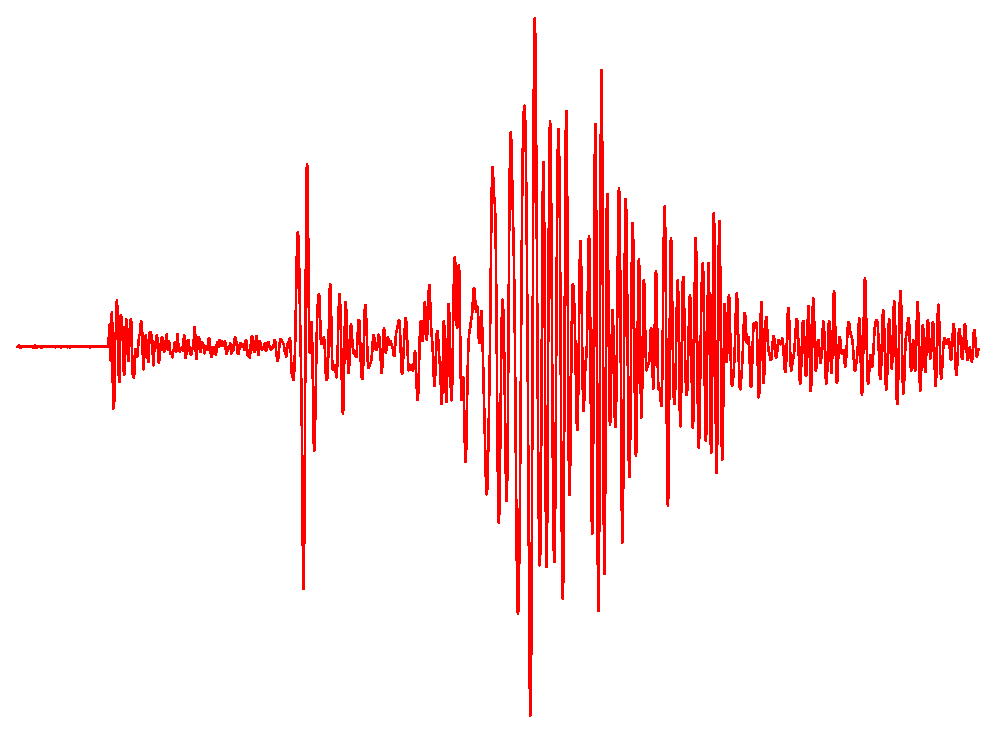
\includegraphics[width=0.8\textwidth]{SAC_logo}\\
\rule{8cm}{0.5mm}\\[0.35cm]
\Huge{\SACDOCTITLE}\\
\rule{8cm}{0.5mm}\\
\Large{\hspace{2.5cm} 基于SAC v\SACVERSION}\\[1cm]

\begin{minipage}{0.8\textwidth}
\begin{flushright}
\begin{tabular}{cl}
\emph{作者:} & \SACDOCAUTHOR \\
\emph{版本:} & \SACDOCVERSION \\
\emph{日期:} & \SACDOCDATE	\\
\end{tabular}
\end{flushright}
\end{minipage}
\end{center}

\end{titlepage}

\pagestyle{empty}

\frontmatter
\section*{\centering 写在第三版前的一些废话}

\begin{shadequote*}
\Large\emph{
工欲善其事,必先利其器。
}
\par\hfill\emph{\normalsize---《论语 $\cdot$ 卫灵公》}
\end{shadequote*}

2010年10月,大三,开始接触并学习SAC;2011年的暑假
开始着手SAC文档的翻译工作;2012年01月,文档的v1.0版本发布;2013年03月
,文档的v2.0版发布。3年多的时间过去了,文档更新到了v3.0版。

v2.0大体上算是官方英文文档的译本,整体结构上完全遵循了官方文档的风格。
整个文档的条理不够清晰,教程部分稍显单薄,命令部分也不够完善。

2013年11月,George Helffrich著的
``\emph{The Seismic Analysic Code : A Primer and User's Guide}''一书出版了。
该书基于MacSAC,与本文档所关注的SAC有一些区别,但是精髓部分是一致的。
v3.0版借鉴了该书的整体结构和部分内容,重新设计了文档结构并重写了教程的大
部分内容,希望能够有一个结构更清晰、内容更丰富的版本。

整个文档分为教程部分和命令部分。教程部分又分为如下几章:
\begin{description}
\item[SAC简介] 简单介绍SAC软件的相关信息;
\item[SAC基础] 继续阅读所需的基础知识;
\item[SAC文件格式] 详细介绍SAC文件格式;
\item[SAC数据处理] 介绍如何利用SAC命令进行地震数据处理和分析;
\item[SAC图像] 介绍如何控制SAC绘制的图像的细节;
\item[SAC编程] 介绍如何用SAC进行数据批处理;
\item[SAC与脚本] 如何在脚本语言(Bash和Perl)中调用SAC;
\item[SAC函数库] 在自己的C或Fortran程序中调用SAC提供的子函数;
\item[SAC I/O] 独立实现SAC I/O子函数;
\item[SAC相关工具] 与SAC有关的一些工具;
\end{description}

对本文档的内容有疑问,或发现任何错误、笔误,欢迎邮件联系我或者在本文档的
GitHub项目主页上提交Issue,也欢迎感兴趣的读者fork该项目,共同完善文档。

此文档仅供个人学习使用,希望不涉及版权问题。

\begin{flushleft}
个人博客: \url{http://seisman.info}                                     \\
项目主页: \url{https://github.com/seisman/SAC_Docs_zh}                  \\
捐赠页面:\url{https://me.alipay.com/seisman}                           \\
文档发布页: \url{http://seisman.info/sac-manual.html}                   \\
联系方式: \url{seisman.info@gmail.com}  

\end{flushleft}

\begin{flushright}
作者~:~SeisMan \\
2014年04月14日
\end{flushright}

\section*{\centering{版本}}

SAC的开发一直在进行,每一个新版本都可能修订一些Bug、加入一些新的特性或
增加新的命令。下表列出了本文档的版本与SAC版本之间的对应关系。就本文档而言,
推荐读者使用SAC的v101.5c或v101.6a版本。

\begin{table}[h]
\centering
\begin{tabular}{c|c|c|c}
\toprule
文档版本		& 	文档发布日期 	& 	SAC版本 &	SAC 发布日期\\
\midrule
1.0  			&	2012-01-08		&	101.4	&	2010-06-07	\\
1.1  			&	2012-09-03		&	101.4	&	2010-06-07	\\
1.2  			&	2012-09-18		&	101.5	&	2011-11-15	\\
2.0  			&	2013-03-29		&	101.5c	&	2012-02-01	\\
2.1  			&	2013-04-06		&	101.5c	&	2012-02-01	\\
2.2  			&	2013-04-12		&	101.5c	&	2012-02-01	\\
2.3             &   2014-02-22      &   101.5c  &   2012-02-01  \\
\SACDOCVERSION  &   \SACDOCDATE     &   \SACVERSION &   \SACDATE    \\
\bottomrule
\end{tabular}
\end{table}


\frontmatter
\pdfbookmark[0]{\contentsname}{contents}
\tableofcontents
\pdfbookmark[0]{\listfigurename}{lof}
\listoffigures
\pdfbookmark[0]{\listtablename}{lot}
\listoftables

\mainmatter
\pagestyle{body}

\part{SAC教程}
\chapter{SAC简介}
\section{SAC是什么?}

Seismic Analysis Code (SAC),是地震学领域使用最广泛的数据分析软件包之一。

SAC首先是一个软件,主要在命令行下工作,通过各种命令来处理时间序列数据
(尤其是地震数据),同时也包含了一个简单的图形界面,使得用户可以方便地查看
波形以及拾取震相。

SAC同时还是一种数据格式,定义了以何种方式存储单个时间序列数据。
SAC格式已经成为了地震学的标准数据格式之一,有很多工具可以实现SAC格式
与其它地震数据格式间的相互转换。

SAC实现了地震数据处理过程中的常用操作,包括重采样、插值、自/互相关、震相拾取、
快速Fourier变换、谱估计、滤波、信号叠加等;同时为了满足数据批处理的需求,
SAC设计了一个基本的编程语言,包括变量、参数、If判断、循环等等
\footnote{SAC设计的基本编程语言,称之为SAC宏,在第\ref{chap:macros}章中会详细
说明,并与Bash和Perl进行对比。}。

\section{SAC发展史}
\label{sec:history}

Lawrence Livermore国家实验室
\footnote{\url{http://en.wikipedia.org/wiki/Lawrence\_Livermore\_National\_Laboratory}}
和Los Alamos国家实验室
\footnote{\url{http://en.wikipedia.org/wiki/Los\_Alamos\_National\_Laboratory}}
是美国承担核武器设计工作的两个实验室。SAC于20世纪80年代诞生于实验室的Treaty Verification Program小组里,该组由W. C. Tapley和Joe Tull共同领导。

起初,SAC是用Fortran语言实现的,并将源代码分发给感兴趣的学者,
允许用户进行非商业性的地震数据处理,
用户和开发者之间的合作协议要求用户提交bug修正和改进以换取SAC的使用权。
到了大概1990年,SAC已经成为全球地震学家的数据处理标准软件。

从1992年开始,SAC的开发逐渐由Livermore接管,并开始通过分发协议严格限制源代码的
分发。与此同时,开发者认为Fortran是一种过于局限的编程语言,其阻碍了SAC特性的进一步
开发,因而开发者使用f2c\footnote{f2c~(\url{http://www.netlib.org/f2c/}),
Fortran77语言到C语言的自动转换工具。}
转换工具将SAC的Fortran源码转换成了C源码\footnote{个人猜测,目前SAC源码的
混乱和不易读正是由于这次自动转换导致的。}。接下来,Livermore以转换得到的
C源码为基础,计划开发一个商业版的地震数据处理产品,命名为SAC2000。
这个版本扩展了很多
功能,其中一个功能是建立一个日志数据库,记录一个波形从原始数据
到最终产品之间的所有处理步骤。这样的设计允许用户暂时保存数据处理步骤,
随时将处理的结果提交到内存或回滚到之前的状态。

约1998年,IRIS\footnote{\url{http://www.iris.edu}}
意识到,SAC的核心用户群(主要是IRIS的成员)无法确保能够
获取SAC的源码。IRIS开始和Livermore协商,希望将SAC的开发分成两条线:一个包含
数据库特性,供核监测机构使用;另一个不包含数据库特性,仅供学术机构使用。
商业化的努力主要集中在含数据库功能的版本上。

终于,在2005年,IRIS与Livermore签订了合同,Livermore提供给IRIS一个SAC协议,
允许其在IRIS社区
内部分享SAC/SAC2000的源代码,并提供有限的支持以促进社区的发展。
而学术圈对于商业版的SAC没有太大兴趣,因而Livermore逐渐撤出了对于SAC2000的支持。
最终IRIS完全接手了SAC的开发和技术支持,并成为了一个新的版本,
也就是我们现在正在使用的SAC,有时为了区分,也称之为SAC/IRIS。
目前的最新版本为101.6a。

\section{SAC变体}

SAC的发展史还是很曲折的,这也导致SAC存在多个不同的变体。

\begin{description}
\item[Fortran SAC]  即SAC的Fortran语言实现。最后一个分发版本发布于2003年,版本号10.6f。
                    曾经以限制性的形式在IASPEI软件库中分发。
\item[SAC2000]      从Fortran源码转换为C源码,并以C源码为基础继续维护。该版本加入了数据库特性以及
                    一些新的命令。目前该版本已不再分发。
\item[SAC/IRIS]     由SAC2000衍生的版本,不包含数据库特性\footnote{目前的SAC/IRIS中还可以看到一些
                    与数据库特性相关的命令和选项,比如很多命令中的commit、rollback、recalltrace选项,
                    这些选项的存在属于历史遗留问题,且已经基本不再维护,因而本文档中完全没有提及。},
                    也就是本文档所使用的版本,在本文档中简称为SAC。
                    现在由IRIS下的SAC开发小组负责维护,并由IRIS分发。
\item[MacSAC]       也称为SAC/BRIS,仅可在Mac OS下使用。该变种由10.6d Fortran源码衍生而来(后期与10.6f集成),
                    其功能是SAC/IRIS功能的超集。相对于SAC/IRIS的最主要扩展在于宏语言功能的增强以及
                    处理台阵数据的能力。其作者为
                    George Helffrich\footnote{\url{http://www1.gly.bris.ac.uk/~george/gh.html}},
                    针对MacSAC写了一本教程
                    \footnote{G.R. Helffrich, J. Wookey \& I.D. Bastow, The Seismic Analysis Code
                    : A Primer and User's Guide. \textsl{Cambridge University Press}, 2013。
                    可以作为学习SAC/IRIS的辅助教程,但需要注意其中可能存在的一些微小差异。}。
\end{description}

\section{安装SAC}
\label{sec:sac-install}
本节介绍如何在Linux下安装SAC,要求读者了解Linux的一些基本概念和操作。

\subsection*{申请SAC}
在``\nameref{sec:history}''中已经说到,SAC协议仅允许在IRIS社区内部分享SAC的源码,
所以SAC不像很多软件一样可以很方便地通过软件包管理器安装或者直接从网络下载源码。

软件包申请地址~:~\url{http://www.iris.edu/ds/nodes/dmc/forms/sac/}

认真填写个人信息,尤其注意Email那一栏,需要填写单位邮箱,如果使用
QQ、163这样的邮箱很容易直接被拒绝,如果没有单位邮箱,需要提供其它
信息以验证你的身份。

IRIS提供了SAC源码包、Linux 64位二进制包和Mac 64位二进制包。对于Linux
用户,可以通过``\lstinline{uname -a}''命令查看当前系统是32位还是64位。对于64位系统,
可以直接使用Linux 64位二进制包;对于Linux 32位系统,则必须手动编译SAC源码。

考虑到在申请提交之后,需要人工审核,两三个工作日后才会通过邮箱获取SAC软件包,
建议还是同时申请Linux 64位二进制包和SAC源码包。

\subsection*{安装依赖包}
Linux下安装软件最麻烦的一个问题就是软件之间的依赖关系。

对于Ubuntu/Debian系\footnote{很久不用Ubuntu,无法保证完全正确。}:
\begin{lstlisting}[style=Shell]
$ sudo apt-get install build-essential
$ sudo apt-get install libncurses5-dev libsm-dev libice-dev
$ sudo apt-get install libxpm-dev libx11-dev zlib1g-dev
\end{lstlisting}

对于CentOS/Fedora/RHEL系:
\begin{lstlisting}[style=Shell]
$ sudo yum groupinstall 'Development Tools'
$ sudo yum install glibc ncurses-devel libSM-devel libICE-devel
$ sudo yum install libXpm-devel libX11-devel zlib-devel
\end{lstlisting}

\subsection*{安装}
安装的方法在这一步分成两个部分,分别是二进制包安装和源代码编译,根据实际情况
二者选一。
\subsubsection*{二进制包安装}
解压sac二进制包:
\begin{lstlisting}[style=Shell]
$ tar -zxvf sac-101.6a-linux_x86_64.tar.gz
\end{lstlisting}

复制sac文件夹到安装目录(推荐安装目录为\lstinline{/usr/local}):
\begin{lstlisting}[style=Shell]
$ sudo cp -r sac /usr/local
\end{lstlisting}

\subsubsection*{源代码编译}
\begin{lstlisting}[style=Shell]
$ tar -zxvf sac-101.6a_source.tar.gz
$ cd sac-101.6a
$ ./configure --prefix=/usr/local/sac
$ make
$ sudo make install
\end{lstlisting}

\subsection*{配置变量}
向~\lstinline{~/.bashrc}~中加入如下语句以配置环境变量和SAC全局变量:
\begin{lstlisting}[style=Bash]
export SACHOME=/usr/local/sac
export SACAUX=$SACHOME/aux
export PATH=$SACHOME/bin:$PATH

export SAC_DISPLAY_COPYRIGHT=1
export SAC_PPK_LARGE_CROSSHAIRS=1
export SAC_USE_DATABASE=0
\end{lstlisting}

其中,
\begin{itemize}
\item \lstinline{SACHOME}~为SAC的安装目录;
\item \lstinline{SACAUX}~中包含了SAC运行所需的辅助文件;
\item \lstinline{PATH}~为Linux系统环境变量;
\item \lstinline{SAC_DISPLAY_COPYRIGHT}~用于控制是否在启动SAC时显示版本和版权信息,
    一般设置为1。在脚本中多次调用SAC时会重复显示版本和版权信息,干扰脚本的正常输出,因而
    在脚本中一般将其值设置为0,设置方法可以参考``\nameref{sec:sac-bash}''、``\nameref{sec:sac-perl}''和``\nameref{sec:sac-python}''
    中的相关内容;
\item \lstinline{SAC_PPK_LARGE_CROSSHAIRS}~用于控制震相拾取过程中光标的大小,在
    ``\nameref{sec:phase-picking}''一节会具体说明;
\item \lstinline{SAC_USE_DATABASE}~用于控制是否允许将SAC格式转换为GSE 2.0格式;
    一般用不到该特性,故而设置其值为0;
\end{itemize}

修改完~\lstinline{~/.bashrc}~后,执行以下命令使配置的环境变量生效:
\begin{lstlisting}[style=Shell]
$ source ~/.bashrc
\end{lstlisting}

\subsection*{启动SAC}
终端键入小写的sac\footnote{Ubuntu的源里有一个名叫sac的软件,是用来显示登录账户
的一些信息;CentOS的源里也有一个名叫sac的软件,是CSS语法分析器的Java接口。所以
一定不要试图用发行版自带的软件包管理器安装sac!!!},显示如下则表示SAC安装成功:
\begin{lstlisting}[style=Shell]
$ sac
 SEISMIC ANALYSIS CODE [11/11/2013 (Version 101.6a)]
 Copyright 1995 Regents of the University of California

SAC>
\end{lstlisting}

\section{邮件组}
邮件组是个好东西,有点我们熟悉的QQ群的味道。在加入了邮件组之后,如果你在使用SAC的过程中
遇到问题,
可以向这个邮件组的邮箱发送HELP邮件,该组内的所有成员都会收到你的邮件。
如果某人知道答案,他或许就会给你回复。发现了SAC的bug也可以向这里报告,开发者会尽快给你回复的。
当然问问题之前要思考
\footnote{请阅读<提问的智慧>\url{http://www.wapm.cn/smart-questions/smart-questions-zh.html}},
提交bug的时候要详细指出bug是如何出现的,也可以给出代码或文件以使得开发者能够重现该bug。

邮件组邮箱~:~\url{sac-help@iris.washington.edu}

订阅地址~:~\small{\url{http://www.iris.washington.edu/mailman/listinfo/sac-help}}


\chapter{SAC基础}
\section{如何学习SAC?}
学习SAC最好的方式是找一个有经验且有耐心的人,让他/她给你演示SAC是如何工作的。
如果没有这样一个人的话,那么你就需要打开终端从头开始自学。

我将SAC的学习过程分成三个阶段,下面列出了每个阶段的具体要求。普通用户需要达到``SAC进阶''
才能满足日常数据处理的要求。

\subsection*{SAC初阶}
\begin{enumerate}
    \item 掌握SAC中最常用的命令,包括但不限于
            \nameref{cmd:help}、
            \nameref{cmd:read}、
            \nameref{cmd:write}、
            \nameref{cmd:plot}、
            \nameref{cmd:quit}、
            \nameref{cmd:plotpk}、
            \nameref{cmd:listhdr}、
            \nameref{cmd:chnhdr}、
            \nameref{cmd:rmean}、
            \nameref{cmd:rtrend}、
            \nameref{cmd:bandpass}、
            \nameref{cmd:plot1}、
            \nameref{cmd:plot2}、
            \nameref{cmd:cut}、
            \nameref{cmd:fft};
        \item 理解地震数据处理流程,参见``~\nameref{chap:data-process}''一章;
        \item 了解~\nameref{chap:sac-file-format},掌握常见的~\nameref{sec:sac-header-variables},
            理解~\nameref{sec:sac-time};
        \item SAC相关工具:\nameref{sec:saclst};
\end{enumerate}

\subsection*{SAC进阶}
\begin{enumerate}
\item 掌握SAC的大部分命令,至少知道SAC可以实现哪些功能;
\item 了解SAC编程以及如何在脚本中调用SAC,见第~\ref{chap:sac-programming}~、~\ref{chap:sac-script}~章;
\item 掌握如何绘制精美的波形图,见第~\ref{chap:sac-graphics}~章;
\item 学会在自己的程序中使用SAC提供的函数库,见第~\ref{chap:sac-libs}~章;
\end{enumerate}

\subsection*{SAC高阶}
\begin{enumerate}
\item 了解SAC软件包的内部结构;
\item 自己写程序实现SAC I/O库;
\item 阅读SAC源码,了解命令的技术细节;
\item 向SAC贡献代码;
\end{enumerate}

\section{如何阅读本文档?}

本文档的内容大体分为两个部分:教程部分和命令部分。命令部分详细的列出了SAC中的
每一个命令的语法、参数以及一些技术细节,适合作为参考,在需要的时候查阅。

教程部分给出了很多日常数据处理的例子,初学者应该坐在计算机前,打开终端,
键入\footnote{严禁复制!不许偷懒!}书中的例子,试着理解每一个步骤的原理以及结果。

在阅读教程的同时,应随时翻看相应命令的说明,在实践的过程中掌握基础命令的语法和用法。
这样基本就完成了SAC初阶的要求。

在读完教程部分之后,应浏览SAC的几乎所有命令,并挑选其中感兴趣的一些进行尝试。此后,
在平常的科研工作中经常使用SAC,有了实践经验和对SAC的进一步认识之后,可以阅读文档
中的进阶内容,达到SAC进阶的要求。

最后,如果对SAC的内部机理感兴趣,可以阅读SAC的源码,重新实现一些SAC底层的功能。

\section{启动和退出}
在终端键入\lstinline{sac}以启动SAC,显示如下版本号以及版权信息
\footnote{Livermore实验室由University of California于1952年创立,2007年改由
University of California、Bechtel National、BWX Technologies、Washington Group International
共同组成的安全机构管理。}
:
\begin{SACCode}
$ sac
 SEISMIC ANALYSIS CODE [11/11/2013 (Version 101.6a)]
 Copyright 1995 Regents of the University of California

SAC> 
\end{SACCode}
其中, ``\lstinline{SAC>}''是SAC程序特有的提示符。

退出SAC:
\begin{SACCode}
SAC> quit
\end{SACCode}
也可以使用\lstinline{done}、\lstinline{exit}命令退出SAC,但不推荐。

\section{SAC设计思想}
SAC的设计思想大概可以总结如下:
\begin{enumerate}
    \item 每个信号\footnote{信号,或称之为trace,即\textbf{单个}台站\textbf{单个}仪器\textbf{单个}分量的数字记录。}
被保存到单独的SAC格式数据文件中;
\item SAC格式包含了描述数据特征的头段区和存储信号的数据区,参见``~\nameref{chap:sac-file-format}~''一章;
\item 将单个或多个\footnote{一次性最多处理\textbf{1000}个任意大小的文件,记住1000这个值!}
    SAC文件从磁盘读入内存;
\item 通过各种命令对内存中的数据进行操作;
\item 操作完毕,将内存中的数据写入到磁盘,可以覆盖原SAC文件或写入新文件中。
\end{enumerate}

\section{SAC命令初探}
\subsection{SAC命令长什么样?}
一个完整的SAC命令一般由``命令+选项+参数''构成,其中命令必须有,选项和参数可以成对
出现,也可以只出现其中一个。命令、选项以及参数之间用空格分开。如果要将多个命令写在
一行,要用分号隔开每个命令。例如:
\begin{SACCode}
SAC> funcgen random delta 0.1 npts 1000
SAC> rmean; rtrend; taper                 // 一行内多个命令用分号隔开
SAC> write rand.SAC
\end{SACCode}
其中,~\lstinline{funcgen}~、~\lstinline{write}~、~\lstinline{rmean}~、~\lstinline{rtrend}~
和~\lstinline{taper}~是命令;~\lstinline{random}~是选项;
~\lstinline{0.1}~是选项~\lstinline{delta}~的参数、~\lstinline{1000}~是选项
~\lstinline{npts}~的参数;而~\lstinline{rand.SAC}~则是一个无选项的参数\footnote{其实
可以有很多选项,这里都省略了。}。

\begin{Tips}
官方文档的原文是``command''、``keyword''和``option'',
本文档v2.0中译为``命令'',``关键字''和``参数''。
个人感觉,无论是官方的用词还是v2.0版的译词都很容易让使用C语言和Linux的人困惑,
因而v3.0中一律将其改为命令(command)、选项(option)和参数(argument)。

这里解释一下选项(option)和参数(argument)的区别。一个命令有哪些选项是由命令规定的,
其控制了命令的一些特性,因而选项的作用是告诉命令``我\textbf{要}改某个特性''。
但是具体\textbf{怎么}改呢?
这个就交给参数来控制了。命令或选项只规定了参数的类型(整型、浮点型、字符串、枚举型或者逻辑型),
用户需要根据自己的需求给定参数值。
\end{Tips}

\subsection{大小写}
SAC的命令和选项都是不区分大小写的,这意味着你可以根据自己的喜好使用~\lstinline{funcgen}~
或者~\lstinline{FUNCGEN}~,SAC在解释命令前都会将其转换为大写字母。

需要注意的是,由于Linux本身是区分大小写的,所以对于出现在参数中的文件名、目录名
或者由引号包围的字符串来说,大小写是完全不同的。比如~\lstinline{rand.SAC}~和
~\lstinline{RAND.SAC}~是两个完全不同的参数。

\subsection{命令简写}
SAC的大多数命令以及选项都有简写形式。比如上面的命令简写形式如下:
\begin{SACCode}
SAC> fg r d 0.1 n 1000
SAC> rmean; rtr; taper
SAC> w rand.SAC
\end{SACCode}

命令和选项究竟可以简写成怎样的形式,是由SAC自身规定的。简写的好处在于,在不产生歧义
的前提下尽量减少用户的击键数;坏处在于,若对命令不是足够熟悉,简写后的命令变得很
难读和难理解。比如你一看就知道~\lstinline{delta}~代表的是采样周期
\footnote{也称为采样时间,即两次数据采样的时间间隔,本文档将统一使用``采样周期''。},
而~\lstinline{d}~却不那么直观,可能是~\lstinline{delta}~,也可能是~\lstinline{demon}~。
所以,简写很好用,但是应该仅用在那些常使用的命令上,不要滥用。

\subsection{查看命令语法}
SAC自带了英文的帮助文档,详细解释了每个命令的语法,可以通过~\lstinline{help}~命令
查看相应文档:
\begin{SACCode}
SAC> help funcgen write   // 命令的简写是h fg w
\end{SACCode}
也可以直接查看~\lstinline{$SACHOME/aux/help}~下的文档,或者查看本文档的命令部分。

\subsection{参数默认值}
为了让SAC易学易用,几乎所有命令参数都有一个``系统默认参数值'',这些``系统默认参数值''
都是经过精心挑选的,
同时用户又可以随时修改参数值。这样的设计使得SAC易用同时又不失灵活性。

下面以C语言为例做一些说明\footnote{有些地方不是很准确。},希望能够帮助理解SAC参数
的一些特点。

在C语言中,函数有主函数和子函数之分,变量又有全局变量和局部变量之分。所有的变量
都可以被初始化为适当的值。

任意一个子函数,都可以使用全局变量的值,即函数的执行可以被全局变量所控制;
同时也可以修改全局变量的值,这使得代码的管理和调试变得困难。一种实际的做法
是定义专门的子函数来修改全局变量。

任意一个子函数,又都有自己的局部变量。这些局部变量在每次子函数被调用时都会被定义、初始化、
使用和赋值,一旦子函数调用结束,变量即被撤销。如果给这些变量加上~\lstinline{static}~
修饰符,则这些局部变量变身为静态局部变量。

静态局部变量,会在程序刚开始的时候就完成初始化,也是唯一的一次初始化。静态局部变量
仅在定义它的子函数里可见,子函数可以任意修改静态局部变量的值,
但是每次子函数调用结束时变量不会被撤销,因此再次调用一个子函数时,静态局部变量的值
可能已经被上一次的子函数调用所修改。

SAC中有与之相对应的一些概念。sac就是一个主函数,每一个命令都是一个子函数。所以SAC
命令可以分为2类:
\begin{description}
\item[操作执行类] 对数据进行某些操作(受全局变量控制,同时又有自己的静态局部变量);
\item[参数设定类] 改变SAC的全局参数值(即C语言中专门用于修改全局变量的子函数); 
\end{description}

在启动SAC(主函数)的时候,所有的选项(C语言中的全局变量和静态局部变量)都会被初始化为
指定的``系统默认参数值''(全局变量和静态局部变量的唯一一次初始化)。

使用参数设定类命令的时候,其修改了SAC的全局参数,会影响接下来与之相关的所有其它
命令的执行效果。使用操作执行类命令的时候,在命令中设定参数,相当于修改静态局部变量的值,不仅会
影响当前命令的执行,也会影响之后所有同名命令的执行。

即:

当你在某个命令中为某个选项指定了一个参数值的时候,该参数值会
成为该命令的该选项的``参数当前值'',该``参数当前值''即成为接下来所有
该命令的该选项的``当前默认值''。

鉴于SAC的这样一个特性,在一次会话中,多次执行同一个命令时,一定需要注意选项的当前值
是多少,因为这可能会影响到后面的一系列结果,这个必须理解和牢记!

\begin{Tips}
当你在一次会话中执行了很多个命令的时候,SAC参数可能已经被弄得一片混乱,
你可以使用~\nameref{cmd:inicm}~命令在不退出SAC的情况下重新初始化。
\end{Tips}

下面用例子解释一下:
\begin{SACCode}
SAC> funcgen
SAC> plot
SAC> funcgen step delta 0.1 npts 1000
SAC> plot
SAC> funcgen boxcar
SAC> plot
\end{SACCode}

\begin{enumerate}
\item 命令~\lstinline{funcgen}~的系统默认值为~\lstinline{funcgen impulse npts 100 delta 1.0 begin 0.}。
\item 第一个~\lstinline{funcgen}~命令没有使用任何选项和参数,其直接使用系统默认值,
    生成一个脉冲数据,并保存到内存中。该数据的起始时间为~\lstinline{0}~,采样周期为~\lstinline{1.0}~,
    数据点数为~\lstinline{100}~。
\item ~\lstinline{plot}~命令会打开一个绘图窗口,并将内存中的数据绘制在窗口中;
\item 第二个~\lstinline{funcgen}~命令生成了一个step函数\footnote{注意:内存中的脉冲函数已经没了。}
    ,并设置其采样周期为~\lstinline{0.1}~,数据点数为~\lstinline{1000}。
\item ~\lstinline{0.1}~和~\lstinline{1000}~分别成为~\lstinline{delta}~和~\lstinline{npts}~的``参数当前值''。
\item 第三个~\lstinline{funcgen}~命令生成了boxcar函数,从绘图结果可以看出~\lstinline{delta}~的值为
    ~\lstinline{0.1}~,~\lstinline{npts}~的值为~\lstinline{1000}~。即继承了上一次命令的参数值。
\end{enumerate}

\section{文档约定}
约定这个事情,说起来容易做起来难,遇到不符合约定的地方只能靠读者自己领悟了。

\subsection*{语法约定}
\begin{enumerate}
\item 命令和选项使用大写字母,参数使用小写字母;
\item 命令和选项均使用全称,简写形式可省略的部分用灰色表示;
\item ``\lstinline{[ ]}''表示该项为可选项;
\item ``\lstinline{A|B|C}''表示A、B、C中任选一项;
\end{enumerate}

示例如下:
\begin{SACSTX}
B!AND!P!ASS! [BU!TTER!|BE!SSEL!|C1|C2] [C!ORNERS! v1 v2] [N!POLES! n] 
    [P!ASSES! n] [T!RANBW! v] [A!TTEN! v]
\end{SACSTX}

\subsection*{示例约定}
\begin{enumerate}
\item 命令、选项、参数均使用小写字母;
\item 常见的命令和选项均使用简写表示;
\item 含有提示符``\lstinline{SAC>}''的行是用户键入的命令,无提示符的行是SAC输出行;
\item 示例中加入注释以帮助用户理解,注释使用了C语言的行注释符号``\lstinline{//}'';
\item 除非上下文说明,否则每个例子都运行在单独的SAC会话中,即每个命令都
    省略了启动sac和退出sac的命令。
\item 除特别情况外,均省略~\nameref{cmd:plot}~命令,用户应该学会随时~\nameref{cmd:plot}~
    以查看当前内存中的波形结果。
\end{enumerate}

示例如下:
\begin{SACCode}
$ sac                           // 该行省略
SAC> fg seis                    // 这是注释
SAC> p                          // 该行省略
SAC> lh o
  
  FILE: SEISMOGR - 1
 --------------

     o = -4.143000e+01
SAC> q                          // 该行省略
\end{SACCode}

\section{样本数据}

想要学习SAC,手头必须有SAC格式的数据,SAC提供了两个命令可以用于生成SAC格式数据,分别是
funcgen和datagen。

\subsection{funcgen}
\nameref{cmd:funcgen}(简写为fg)表示``function generator'',即该命令可以生成一些特定的函数,
比如脉冲、阶跃、正弦等等,还可以生成一个地震波形样本。
\begin{SACCode}
SAC> fg impulse         // 生成脉冲函数
\end{SACCode}
上面的命令生成了一个脉冲函数并存储在SAC的内存中,可以用命令~\nameref{cmd:plot}
(简写为p)在图形界面上查看这个函数的样子:
\begin{SACCode}
SAC> p
\end{SACCode}
在学习SAC的过程中,~\nameref{cmd:funcgen}~可以生成地震波形样本:
\begin{SACCode}
SAC> fg seismogram      // 生成地震波形样本,简写为fg seis
\end{SACCode}
这个命令在SAC内存中产生了一个地震波形样本\footnote{此命令的本质就是
读取~\lstinline{$SACAUX}~目录中的~\lstinline{seismogram}~文件到内存。},
同时删除了内存中刚才生成的脉冲信号,可以使用~\nameref{cmd:plot}~命令查看地震波形。
这个地震波形样本在以后的教程中经常用到。

\subsection{datagen}
\nameref{cmd:datagen}(简写为dg)表示``data generator''。顾名思义,就是用来生成
数据的。

下面的例子在内存中生成了CDV台站记录到的一个近震的三分量波形数据
\footnote{此命令本质上就是从~\lstinline{$SACAUX/datagen}~目录中
读取SAC文件到内存。}
,并用~\nameref{cmd:plot1}~(简写p1)将三个波形画在一张图上:
\begin{SACCode}
SAC> dg sub local cdv.n cdv.e cdv.z
SAC> p1 
\end{SACCode}
简单解释一下,datagen命令中,sub为选项,其参数可以取~\lstinline{local}~、
~\lstinline{regional}~、~\lstinline{teleseism}~,对应近震、区域震和远震,分别又可以
使用不同的参数以读取不同台站的SAC数据。具体参考~\nameref{cmd:datagen}~。

p1会将内存中的所有文件(本例中是3个)同时绘制在一张图上,当内存中的文件数目很多
时,需要修改p1的其它参数,以控制每张图上显示的波形数目。

\section{SAC的读和写}
SAC的读命令是~\nameref{cmd:read}(简写为r),写命令为~\nameref{cmd:write}(简写为w)。
读和写是紧密联系的,所以把这两者放在一起讲。

注意:本节的所有示例都运行在同一个SAC会话中。

要演示如何读SAC文件,首先得有一些SAC数据才行,利用上一节的datagen生成一些数据。
\begin{SACCode}
$ ls                // 空文件夹
$ sac               // 启动一个SAC会话
 SEISMIC ANALYSIS CODE [11/11/2013 (Version 101.6a)]
 Copyright 1995 Regents of the University of California

SAC> dg sub local cdv.n cdv.e cdv.z     // 生成三个SAC数据
SAC> w cdv.n cdv.e cdv.z                // 将SAC数据写入磁盘
SAC> ls                                 // 在SAC中也可以使用一些常见的系统命令
cdv.e  cdv.n  cdv.z
\end{SACCode}

有了数据之后,就可以练习如何去读了,在读数据之前,先说一说通配符的概念。

SAC中,在指定文件名的时候,可以使用绝对路径,也可以使用相对路径。可以使用
其全名,也可以使用通配符。SAC的通配符与Unix定义的通配符一致,只包含如下三种:
\begin{enumerate}
\item ``\lstinline{*}'' 匹配任意长度的字符串(包括零长度);
\item ``\lstinline{?}'' 匹配任意单个非空字符;
\item ``\lstinline{[]}'' 匹配列表中的任意单一字符;
    \begin{itemize}
        \item ``\lstinline{[ABC]}'' 匹配单个字符A或B或C
        \item ``\lstinline{[A,B,C]}'' 匹配单个字符A或B或C
        \item ``\lstinline{[0-9]}'' 匹配任意一位数字
        \item ``\lstinline{[a-g]}'' 匹配从a到g范围内的任意单个字符
    \end{itemize}
\end{enumerate}

下面的例子展示了如何读取SAC文件:
\begin{SACCode}
SAC> r cdv.n cdv.e cdv.z    // 读入三个文件,分别指定其文件名
SAC> r cdv.?                // 问号可以匹配单个字符。
./cdv.e ...cdv.n ...cdv.z   // 注意!这里文件读入的顺序与上一个命令不同
SAC> r cdv.[nez]            // 还可以这样读
./cdv.e ...cdv.n ...cdv.z
SAC> r *                    // 也可以这样读
./cdv.e ...cdv.n ...cdv.z
\end{SACCode}

需要注意的是,SAC在每次执行读取命令时,都会读入新的波形数据,并删除内存中原有的
波形数据,所以经过上面四次read之后,内存中依然只有三个波形。

当然,read也有选项,使得读取时将波形追加到内存中的波形数据集之后,而不替换
内存中的原有波形:
\begin{SACCode}
SAC> r ./cdv.n              // one file       0 -> 1
SAC> r more ./cdv.e         // one MORE file  1 -> 2
SAC> r more ./cdv.z         // one MORE file  2 -> 3
\end{SACCode}

将数据读入到内存中之后,对内存中的数据做一些处理,然后就需要将内存中的数据
写回到磁盘中:
\begin{SACCode}
SAC> w test.n test.e test.z         // 分别写入到三个新文件中
SAC> w over                         // 覆盖磁盘原文件
SAC> w append .new                  // 在原文件名的基础上加上后缀".new"
cdv.e.new cdv.n.new cdv.z.new
SAC> ls
cdv.e  cdv.e.new  cdv.n  cdv.n.new  cdv.z  cdv.z.new  tesn.n  test.e  test.z
\end{SACCode}

\section{绘图}
\label{sec:display}

SAC中有四个常用的绘图命令,分别是~\nameref{cmd:plot}、\nameref{cmd:plot1}、\nameref{cmd:plot2}、
\nameref{cmd:plotpk}。

plotpk用于``人机交互''过程中拾取震相,在``~\nameref{sec:phase-picking}~''一节中会详细讲解。

下面说说plot、plot1和plot2的区别。

当内存中只有一个波形的时候,这三个绘图命令是没有区别的,这种情况下一般直接使用
plot;而当内存中存在多个文件时,这三个命令的区别就非常明显了。

\subsection{plot}
\label{subsec:plot}
plot命令会在单个图形窗口中显示单个波形。
\begin{SACCode}
SAC> r cdv.[nez]
SAC> p
Waiting
Waiting
SAC>
\end{SACCode}

鉴于在SAC绘图中有很多中文意思类似的名词,这里似乎有必要定义一下``窗口''。图
\ref{fig:plot}~展示了一个SAC窗口。同很多其它软件界面类似,这个窗口在左上角显示
图标,右上角显示``最小化''、``最大化''、``还原''和``关闭''按钮。

左上角的``Graphics Window: 1''指明了当前绘图窗口的编号为``1''。SAC中一共可以同时
使用10个类似的窗口。

窗口的中间部分为真正的绘图区,以后的图将只显示绘图区而不显示整个窗口。

\begin{figure}[H]
\centering
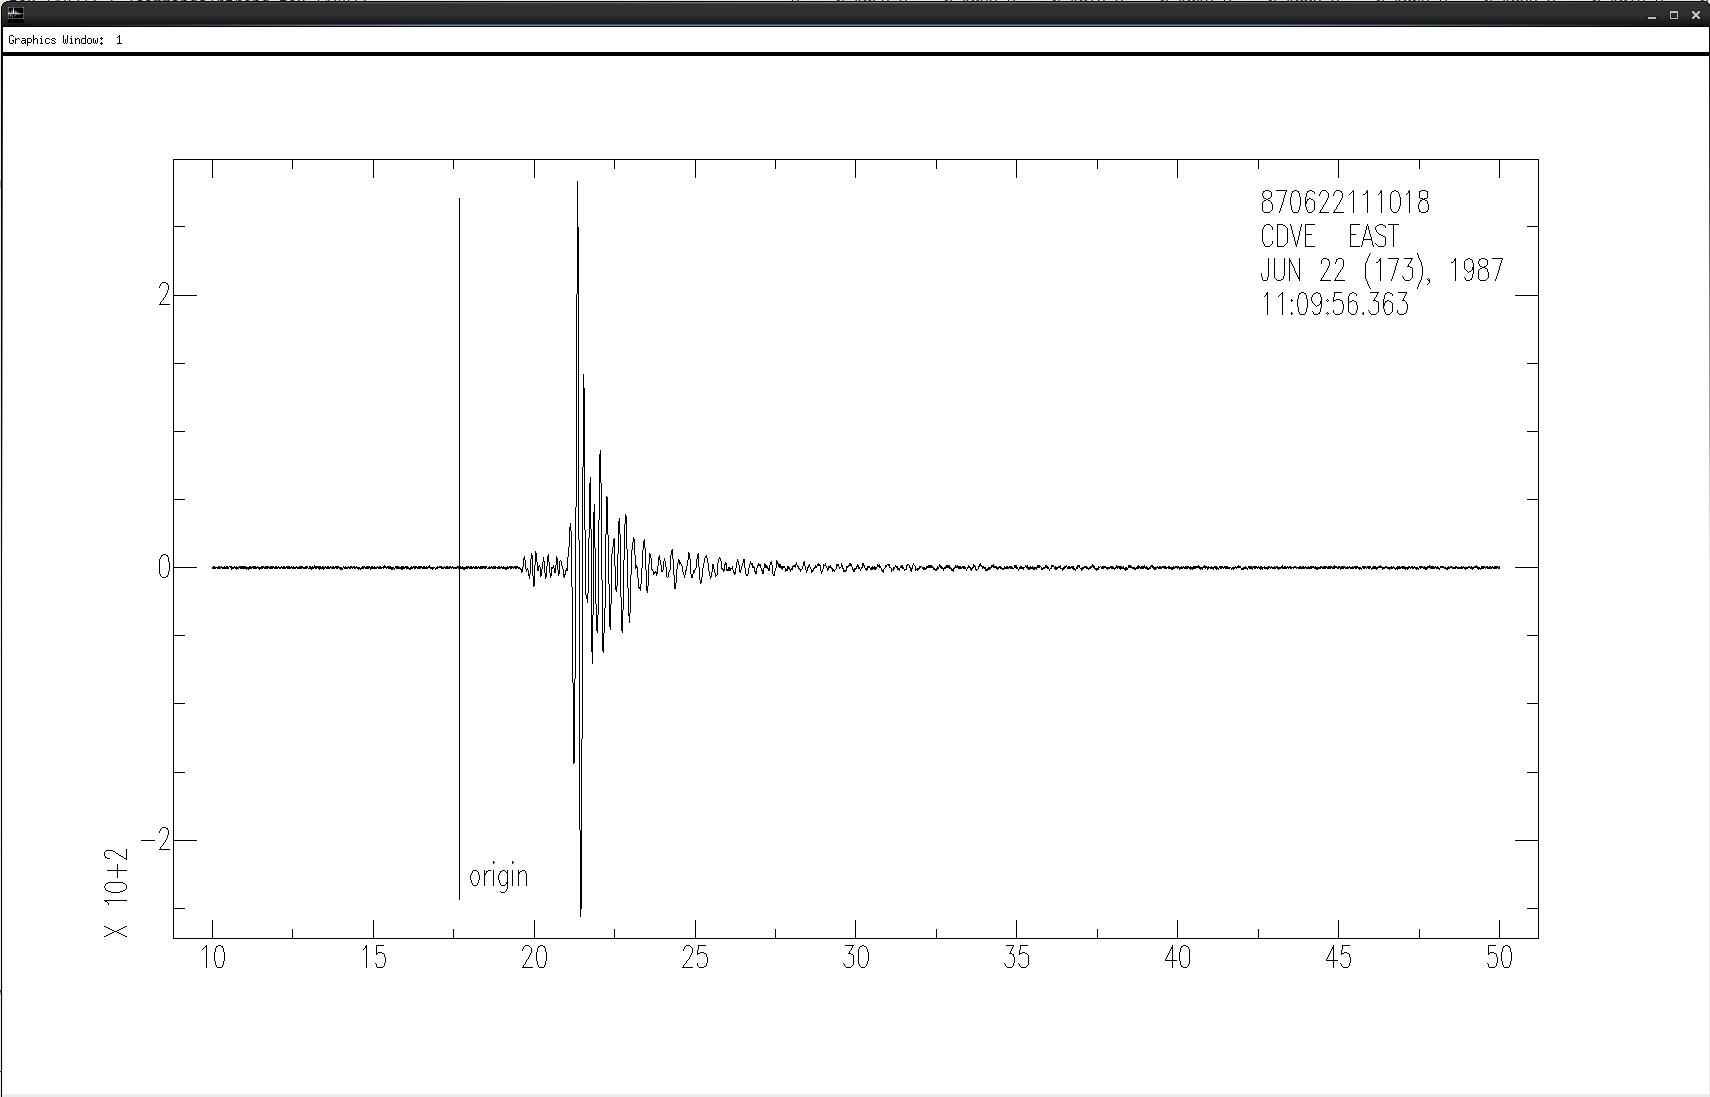
\includegraphics[width=0.9\textwidth]{plot}
\caption{绘图窗口}
\label{fig:plot}
\end{figure}

将三个波形数据读入内存,使用plot时,焦点位于绘图窗口,且绘图窗口上只显示
第一个波形,终端中出现``Waiting''字样;将焦点切换\footnote{Linux下的快捷键是Alt+Tab。}回终端,
敲击回车键,绘图窗口中显示第二个波形,终端中出现第二个``Waiting''字样,
焦点位于终端中;再次敲击回车键,窗口中显示第三个波形,焦点位于终端,
由于已经没有更多的波形需要显示,此时终端中显示SAC提示符。

如果内存中还有波形在``Waiting'',而你想要退出plot,不想要再继续查看后面的波形,
可以在终端中键入``kill''(简写为k),以直接退出plot,如下例:
\begin{SACCode}
SAC> r cdv.[nez]
SAC> p
Waitingk
SAC>
\end{SACCode}

也许你已经发现,即使plot结束或者中途退出plot,绘图窗口依然没有被关闭,而且即便
点击窗口的``关闭''按钮,窗口依然无法关闭。
\begin{SACCode}
SAC> r cdv.[nez]
SAC> begindevices xwindows      // 启动图像设备xwindows,简写为bd x
SAC> p
Waiting
Waiting
SAC> enddevices xwindows        // 关闭图像设备xwindows,简写为ed x
\end{SACCode}
严格地说,SAC绘图的流程应该是:启动图像设备(xwindows或者sgf)$\rightarrow$绘图$\rightarrow$关闭图像设备。
这样稍显繁琐,SAC将这一流程进行了简化,在每次绘图前偷偷启动了SAC默认的图像设备xwindows,
也就是上面所说的窗口,而关闭图像设备这一步需要用户自己完成,当然,在退出SAC时,SAC
也会自动关闭图像设备。

\subsection{plot1}
plot1命令会在一个窗口中显示多个波形。这些波形共用一个X轴,但拥有单独的Y轴。
\begin{SACCode}
SAC> r cdv.?
cdv.e cdv.n cdv.z
SAC> p1
\end{SACCode}
执行plot1命令后,焦点位于图形窗口,显示如图~\ref{fig:plot1}。
\begin{figure}[H]
\centering
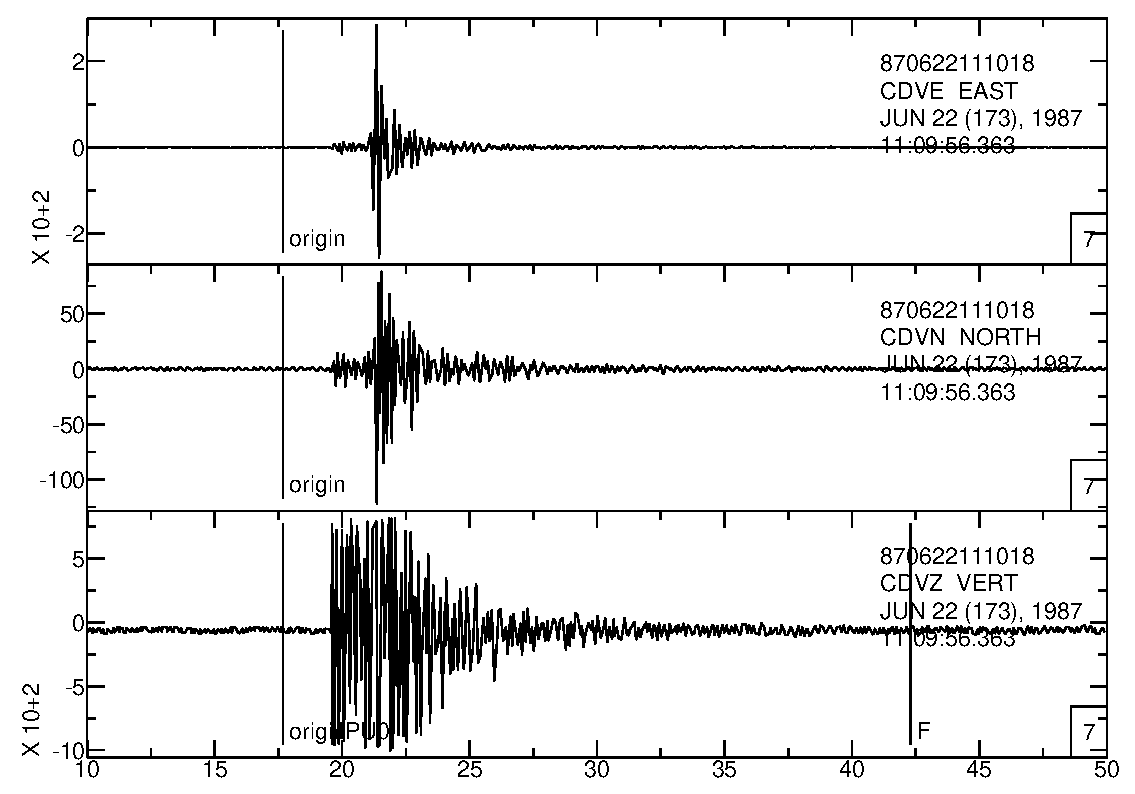
\includegraphics[width=\textwidth]{plot1}
\caption{plot1绘图效果}
\label{fig:plot1}
\end{figure}




\chapter{SAC文件格式}
\section{SAC格式简介}
一个地震波形数据包含了时间上连续的一系列数据点,数据点可以是等间隔或不等间隔采样。
SAC的数据格式要求一个文件中只包含一个地震波形数据,这样的定义更适合单个地震波形的处理。

每个SAC文件包含两个部分:一个头段区和一个数据区。

头段区位于每个文件的起始处,其大小是固定的,用于描述数据的相关信息,比如数据点数、
采样周期等等。

数据区紧跟在头段区之后,数据区又包含了一个或多个子数据区:
\begin{itemize}
\item 如果数据是时间序列,且是等间隔采样的,则只有一个子数据区,包含因变量(Y,也就是数据)的值,
    因变量(X)的信息可以直接从头段区中获得;
\item 如果数据是时间序列,但是不等间隔采样的,则有两个子数据区,分别包含因变量(Y)和自变量(X)
    的值;
\item 如果数据是谱数据而非时间序列,则有两个子数据区,分别包含振幅和相位或者实部和虚部;
\item 如果数据是三维数据(XYZ),则包含NXSIZE*NYSIZE个子数据区。
\end{itemize}

\section{两种数据形式}
SAC文件格式有两种形式:二进制型和字符型\footnote{原为alphanumeric,译为文数字。}。

字符型与二进制型是完全等价的,只是字符型是给人看的,二进制型是给机器读写的。从C
程序的角度来看,两者的区别在于,写文件时前者使用~\lstinline{fprintf}~后者使用
~\lstinline{fwrite}~。

二进制型的SAC数据,占用更小的磁盘空间,读写速度更快,因而是最常用的SAC格式形式。

字符型适合于在文件出现问题时,临时查看文件内容的时候使用。

\subsection{两种形式的互相转换}
你是否想要一个字符型的SAC文件,用编辑器打开好好看看SAC数据究竟长什么样。SAC自带
的命令可以实现两种形式的转换
\footnote{也可以使用SAC的~\lstinline{convert}~命令进行转换,不过此命令即将被淘汰。}
。
\begin{SACCode}
SAC> fg seis
SAC> w seis             // 先生成一个二进制型SAC数据,以做测试
\end{SACCode}

将二进制型转换成字符型:
\begin{SACCode}
SAC> r seis             // 读二进制型文件
SAC> w alpha seis.a     // 以字符型写入
\end{SACCode}

将字符型转换成二进制型:
\begin{SACCode}
SAC> r alpha seis.a     // 读字符型文件
SAC> w sac seis.b       // 以二进制型写入,可以省略sac,写成w seis.b
\end{SACCode}

试试用你最喜欢的文本编辑器打开字符型的~\lstinline{seis.a}~吧,其内容如下:
\begin{lstlisting}[style=Bash]
     0.01000000      -1.569280       1.520640      -12345.00      -12345.00
       9.459999       19.45000      -41.43000       10.46400      -12345.00
      -12345.00      -12345.00      -12345.00      -12345.00      -12345.00
      -12345.00      -12345.00      -12345.00      -12345.00      -12345.00
      -12345.00      -12345.00      -12345.00      -12345.00      -12345.00
      -12345.00      -12345.00      -12345.00      -12345.00      -12345.00
      -12345.00       48.00000      -120.0000      -12345.00      -12345.00
       48.00000      -125.0000      -12345.00       15.00000      -12345.00
      -12345.00      -12345.00      -12345.00      -12345.00      -12345.00
      -12345.00      -12345.00      -12345.00      -12345.00      -12345.00
       373.0627       88.14721       271.8528       3.357465      -12345.00
      -12345.00    -0.09854718       0.000000       0.000000      -12345.00
      -12345.00      -12345.00      -12345.00      -12345.00      -12345.00
      -12345.00      -12345.00      -12345.00      -12345.00      -12345.00
      1981        88        10        38        14  
         0         6         0         0      1000
    -12345    -12345    -12345    -12345    -12345
         1        50         9    -12345    -12345
    -12345    -12345        42    -12345    -12345
    -12345    -12345    -12345    -12345    -12345
    -12345    -12345    -12345    -12345    -12345
         1         1         1         1         0   
CDV      K8108838    
-12345  -12345  -12345  
-12345  -12345  -12345  
-12345  -12345  -12345  
-12345  -12345  -12345  
-12345  -12345  -12345  
-12345  -12345  -12345  
-12345  -12345  -12345  
    -0.09728001    -0.09728001    -0.09856002    -0.09856002    -0.09728001
    -0.09600000    -0.09472002    -0.09344001    -0.09344001    -0.09344001
    -0.09344001    -0.09344001    -0.09472002    -0.09472002    -0.09344001
    ......
\end{lstlisting}

第1-30行是头段区,31及以后N行是数据区。
目前你可能还看不懂头段区的这些数字或者字符代表什么。没关系,在下一节会详细介绍
SAC头段区,记得一定要一边看下一节的内容,一边对照着这个例子,好好琢磨SAC的头段。

\section{SAC头段结构}
SAC头段区长度为632个字节,由一系列头段变量构成。从这些头段变量中可以了解到波形
记录的很多信息,比如台站经纬度、发震时刻、震相到时等等。

表\ref{table:header-variables}列出了SAC头段区的全部头段变量。其中变量名为
\lstinline{internal}表示该变量为SAC内部使用的头段变量,用户不可对其进行操作。
变量名为\lstinline{unused}表示该变量暂时尚未使用,为以后可能出现的新头段变量占位。

\begin{table}[H]
\ttfamily
\small
\centering
\caption{SAC头段变量列表}
\label{table:header-variables}
\begin{tabular}{c|c|lllll}
	\toprule
    Byte	&	Type	&	\multicolumn{5}{c}{Names}\\
	\midrule
	0		&	F	&	delta	&	depmin	&	depmax	&	scale	&	odelta	\\
	20		&	F	&	b		&	e		&	o		&	a		&	internal\\
	40		&	F	&	t0		&	t1		&	t2		&	t3		&	t4		\\
	60		&	F	&	t5		&	t6		&	t7		&	t8		&	t9		\\
	80		&	F	&	f		&	resp0	&	resp1	&	resp2	&	resp3	\\
	100		&	F	&	resp4	&	resp5	&	resp6	&	resp7	&	resp8	\\
    120		&	F	&	resp9	&	stla	&	stlo	&	stel	&	stdp	\\
	140		&	F	&	evla	&	evlo	&	evel	&	evdp	&	mag		\\
	160		&	F	&	user0	&	user1	&	user2	&	user3	&	user4	\\
	180		&	F	&	user5	&	user6	&	user7	&	user8	&	user9	\\
	200		&	F	&	dist	&	az		&	baz		&	gcarc	&	internal\\
	220		&	F	&	internal&	depmen	&	cmpaz	&	cmpinc	&	xminimun\\
	240		&	F	&	xmaximum&	yminimum&	ymaximum&	unused	&	unused	\\
	260		&	F	&	unused	&	unused	&	unused	&	unused	&	unused	\\
	280		&	N	&	nzyear	&	nzjday	&	nzhour	&	nzmin	&	nzsec	\\
	300		&	N	&	nzmsec	&	nvhdr	&	norid	&	nevid	&	npts	\\
	320		&	N	&	internal&	nwfid	&	nxsize	&	nysize	&	unused	\\
	340		&	I	&	iftype	&	idep	&	iztype	&	unused	&	iinst	\\
	360		&	I	&	istreg	&	ievreg	&	ievtyp	&	iqual	&	isynth	\\
    380		&	I	&	imagtyp &	imagsrc	&	unused	&	unused	&	unused	\\
	400		&	I	&	unused	&	unused	&	unused	&	unused	&	unused	\\
	420		&	L	&	leven	&	lpspol	&	lovrok	&	lcalda	&	unused	\\
	440		&	K	&	kstnm	&	kevnm*	&			&			&			\\
	464		&	K	&	khole	&	ko		&	ka		&			&			\\
	488		&	K	&	kt0		&	kt1		&	kt2		&			&			\\
	512		&	K	&	kt3		&	kt4		&	kt5		&			&			\\
	536		&	K	&	kt6		&	kt7		&	kt8		&			&			\\
	560		&	K	&	kt9		&	kf		&	kuser0	&			&			\\
	584		&	K	&	kuser1	&	kuser2	&	kcmpnm	&			&			\\
	608		&	K	&	knetwk	&	kdatrd	&	kinst	&			&			\\
    \bottomrule
\end{tabular}
\end{table}

表\ref{table:header-variables}中,给出了头段区的全部头段变量,在源代码中,其被定义
为一个结构体,结构体中变量\lstinline{delta}开始于第零个字节,占据4个字节,
\lstinline{depmin}开始于第4个字节,也占据4个字节,其它同理。表中的第一列给出了
当前行的第一个头段变量的起始字节数。
第二列给出了头段变量的类型码,每个头段变量类型码对应的数据类型见表
\ref{sec:header-variables-type}。

表\ref{sec:header-variables-type}中,第一列为头段变量类型代码,第二类给出了其
代表的变量类型,第三列指出C源码中该变量的是用什么类型定义的,第四列给出了
写字符形式SAC文件时的输出格式。对于一个SAC文件,并非所有的头段变量都必须要包含
有意义的值,若变量未定义称其包含未定义值,第5列给出了不同类型的未定义值的形式,
比如如果一个整型头段变量的值为-12345,则认为其处于未定义态。实际使用的时候,SAC
提供了参数\lstinline{undef},其可以根据头段变量的类型自动转换成相应类型的未定义值。

SAC中定义了6种头段变量类型,分别为浮点型(F)、整型(N)、枚举型(I)、逻辑型(L)、字符型(K)和辅助型(A)。
其中辅助型不存在于SAC文件中,其直接由其它头段变量推导得到。

除了F型变量外以外,其余所有变量的变量名均以变量类型码开头,比如\lstinline{nvhdr}
是N型变量,\lstinline{leven}是L型变量。

枚举型变量,本质上是\lstinline{int}型,其只能在固定的几个值中取值;C语言中本身
是没有规定Bool类型的,SAC自定义了true和false,用于表示真和假。字符型变量长度为
8,只有\lstinline{kevnm}很特殊,其长度为16。

\begin{table}[H]
\caption{变量类型说明}
\label{table:header-variables-type}
\centering
\ttfamily
\small
\begin{tabular}{cllcll}
	\toprule
    Code    &	Type        &   C Type & sizeof &   printf	&   未定义值        \\
	\midrule
    F		&	浮点型		&   float  &  4     &	\%15.7f &   -12345.0        \\
    N		&	整型		&   int    &  4     &	\%10d   &   -12345        \\
    I		&	枚举型		&   int    &  4     &	\%10d   &   -12345	        \\
    L		&	逻辑型		&   int    &  4     &	\%10d   &   FALSE        \\
    K		&	字符型		&   char*  &  8     &	\%-8.8s & \lstinline[showspaces=true]{"-12345  "}     \\
    A		&	辅助型		&          &        &			& 	    \\
	\bottomrule
\end{tabular}
\end{table}

\section{熟悉头段变量}

\subsection{基本变量}
\begin{table}[H]
\centering
\caption{}
\label{}
\begin{tabular}{ccl}
    \toprule
	变量名	&	类型	&	描述\\
	\midrule
    nvhdr*\footnote{星号表示SAC文件中必须定义该变量}	&	N		&	SAC头段版本号,目前值为6,旧版本的SAC文件($nvhdr<6$)在读入时会自动更新。\\
	nzyear	&	N 		&	GMT年,文件参考时间	\\
    nzjday  &   N       &   GMT儒略日,一年中的第几天\footnote{比``月-日''少用一个变量。}    \\
    nzhour  &   N       &   GMT时   \\
    nzmin   &   N       &   GMT分   \\
    nzsec   &   N       &   GMT秒   \\
    nzmsec  &   N       &  GMT毫秒  \\
	nzdttm	&	N 		&	GMT日期-时间数组,不在头段中,用于子程序读取SAC文件。该数组由上面6个变量构成    \\
	kzdate	&	A		&	不在头段中,字母数字格式的GMT参考日期,由NZYEAR和NZJDAY导出\\
	kztime	&	A		&	不在头段中,字母数字格式的GMT参考时间,由NZHOUR, NZMIN, NZSEC和NZMSEC导出\\
	iftype*	&	I		&	文件类型:\\
						&& \quad- ITIME 时间序列文件	\\
						&& \quad- IRLIM 频谱文件实部-虚部格式 \\
 						&& \quad- IAMPH 频谱文件振幅-相位格式	\\
						&& \quad- IXY 一般的x-y数据 	\\
						&& \quad- IXYZ 一般的XYZ(3-D)文件\\	
	idep	&	I		&	因变量类型:\\
						&& \quad- IUNKN (未知)	\\
						&& \quad- IDISP (位移:nm)	\\
						&& \quad- IVEL (速度:nm/sec)	\\
						&& \quad- IVOLTS (速度:volts)	\\
						&& \quad- IACC (加速度:nm/sec/sec)	\\
	iztype	&	I 		&	等效参考时间	\\
						&& \quad- IUNKN (未知)	\\
						&& \quad- IB (文件开始时间)	\\
						&& \quad- IDAY (基准GMT的午夜)	\\
						&& \quad- IO (事件发生时间)	\\
						&& \quad- IA (初动到时)	\\
						&& \quad- ITn (用户自定义的读取时间Tn, n=0,9)	\\
    \bottomrule
\end{tabular}
\end{table}

\subsection{数据相关变量}
\begin{table}[H]
\centering
\caption{}
\label{}
\begin{tabular}{ccc}
    \toprule
	变量名	&	类型	&	描述\\
	\midrule
    npts*	&   N		&	数据点数。\\
	delta*	&	F		&	等间隔数据的采样间隔(标称值)。\\
	DEPMIN	&	F 		&	因变量最小值。	\\
	DEPMAX	&	F		&	因变量最大值	\\
	DEPMEN	&	F		&	因变量平均值	\\
	SCALE	&	F		&	因变量比例因子\footnote{真实物理场被乘以比例因子得到现有数据}	\\
	ODELTA*	&	F		&	采样间隔的观测值,若观测值与标称值不同则有值\\
	B*		&	F		&	自变量起始值(相对参考时间的秒数)\\
	E*		&	F		&	自变量结束值(相对参考时间的秒数)\\
    XMINIMUM&   F       &   X的最小值(限于谱文件)   \\                                                                                                    
    XMAXIMUM&   F       &   X的最大值(限于谱文件)   \\                           
    YMINIMUM&   F       &   Y的最小值(限于谱文件)   \\                           
    YMAXIMUM&   F       &   Y的最大值(限于谱文件)   \\  
    NXSIZE  &   N       &   频谱长度(限于谱文件)    \\                           
    NYSIZE  &   N       &   频谱宽度(限于谱文件)    \\
    IQUAL   &   I       &   数据质量[未使用]:   \\                                                                                                        
                        && - IGOOD (Good data)  \\                               
                        && - IGLCH (Glitches)   \\                               
                        && - IDROP (Dropouts)   \\                               
                        && - ILOWSN (Low signal to noise ratio) \\               
                        && - IOTHER (Other)\\                                    
    ISYNTH  &   I       &   合成数据标识[未使用]:\\                              
                        && - IRLDTA (Real data) \\                               
                        && - ????? (Flags for various synthetic seismogram codes) \\
     LEVEN*  &   L       &   若数据为等间隔则为TRUE。\\
    \bottomrule
\end{tabular}
\end{table}

\subsection{事件相关变量}
\begin{table}[H]
\centering
\caption{}
\label{}
\begin{tabular}{ccc}
    \toprule
	变量名	&	类型	&	描述\\
	\midrule
    KEVNM   &   K       &   事件名  \\
    IEVREG  &   I       &   事件地理区域[未使用]    \\
    IEVTYP  &   I       &   事件类型    \\
    EVLA    &   F       &   事件纬度(度,北为正) \\                                                                                                        
    EVLO    &   F       &   事件经度(度,东为正) \\                                  
    EVEL    &   F       &   事件高程(m). [未使用]   \\                              
    EVDP    &   F       &   事件相对地表深度(m). [未使用]   \\                   
    MAG     &   F       &   事件震级    \\                                       
    IMAGTYP &   I       &   震级类型:\\                       
    IMAGSRC &   I       &   震级来源信息:   \\
    NEVID   &   N       &   事件ID (CSS 3.0)    \\
    NORID   &   N       &   起始时间ID (CSS 3.0)    \\ 
    NWFID   &   N       &   波形ID (CSS 3.0)    \\ 
    KHOLE   &   K       &   核爆事件:孔眼标识;其他:位置标识  \\
    GCARC   &   F       &   台站到事件的大园弧长,即另一种震中距(度).\\ 
    DIST    &   F       &   事件台站距离,即震中距(km)\\                         
    AZ      &   F       &   事件到台站的方位角(度).\\                                                                                                     
    BAZ     &   F       &   台站到事件的方位角(度). \\                           
    O       &   F       &   事件发生时间(相对参考时间的秒数)    \\                                                                                        
    KO      &   A       &   事件发生时间标志    \\  
    \bottomrule
\end{tabular}
\end{table}

\subsection{台站相关变量}
\begin{table}[H]
\centering
\caption{}
\label{}
\begin{tabular}{ccc}
    \toprule
	变量名	&	类型	&	描述\\
    \midrule
    KNETWK  &   K       &   地震台网名  \\
    KSTNM   &   K       &   台站名      \\      
    ISTREG  &   I       &   台站地理区域[未使用]    \\  
    STLA    &   F       &   台站纬度(度,北为正)    \\                           
    STLO    &   F       &   台站经度(度,东为正).   \\                           
    STEL    &   F       &   台站高程(m). [未使用]\\                              
    STDP    &   F       &   台站相对地表深度(m). [未使用]\\                      
    CMPAZ   &   F       &   分量方位角(从北开始顺时针度数).\\                    
    CMPINC  &   F       &   分量倾角(从垂直开始的度数)  \\    
    KCMPNM  &   K       &   分量名称,SEED格式使用那个三字符名称,第三个代表分量的方位(如BHE),
                            对于水平分量,目前的趋势是使用1和2代替N和E  \\ 
    KSTCMP  &   A       &   台站分量,由KSTNM, CMPAZ和CMPINC导出\\
    LPSPOL  &   L       &   如果台站分量为正极性则为真(左手规则)  \\
    \bottomrule
\end{tabular}
\end{table}

\subsection{震相相关变量}
\begin{table}[H]
\centering
\caption{}
\label{}
\begin{tabular}{ccc}
    \toprule
	变量名	&	类型	&	描述\\
    \midrule
    A       &   F       &   初动到时(相对参考时间的秒数)\\                       
    KA      &   K       &   初动到时标志    \\                                                                                                            
    F       &   F       &   事件结束时间(相对参考时间的描述,注意与文件结束时间的区别)\\
    KF      &   A       &   事件结束标志    \\                                   
    Tn      &   F       &   用户定义的时间,在拾取震相时使用,n = 0-9(相对参考时间的秒数)\\
    KTn     &   K       &   用户定义的时间标志, n = 0-9.    \\ 
    \bottomrule
\end{tabular}
\end{table}

\subsection{仪器相关变量}
\begin{table}[H]
\centering
\caption{}
\label{}
\begin{tabular}{ccc}
    \toprule
	变量名	&	类型	&	描述\\
    \midrule
    KINST   &   K       &   记录仪器通用名称    \\                               
    IINST   &   I       &   记录仪器类型[未使用]\\                               
    RESPn   &   F       &   仪器响应参数,n=0,9. [未使用]\\
    \bottomrule
\end{tabular}
\end{table}

\subsection{其它变量}
\begin{table}[H]
\centering
\caption{}
\label{}
\begin{tabular}{ccc}
    \toprule
	变量名	&	类型	&	描述\\
    \midrule
    USERn   &   F       &   用户定义变量存储区, n = 0,9.\\
    KUSERn  &   K       &   用户定义变量存储区,  n = 0,9.\\     
    LOVROK  &   L       &   如果文件可覆盖则为真,类似于写权限  \\  
    LCALDA  &   L       &   如果DIST, AZ, BAZ 和 GCARC可以由台站和事件的坐标计算出来则为真\\
    KDATRD  &   K       &   数据被读入计算机的日期\\ 
    \bottomrule
\end{tabular}
\end{table}

\section{SAC中的时间概念}
\label{sec:sac-time}

\subsection{基本思路}
SAC的头段区有很多与时间相关的头段变量,包括nzyear、nzjday、nzhour、nzmin、nzsec、
nzmsec、b、e、o、a、f、tn(n=0-9),正确使用它们的前提是理解SAC中的时间概念。
这一节将试着说清楚这个问题。

首先,SAC处理的是地震波形数据,SAC格式里保存的是时间序列数据。先不管其它的一些台站
经纬度、事件经纬度信息,就数据而言,至少需要一系列数据值以及每个数据值所对应的时刻。

在本节接下来的内容中,将严格区分两个高中物理学过的概念:时刻和时间。简单地说,
在时间轴上,时刻是一个点,时间是一个线段。

一个简单的例子如下:
\begin{lstlisting}[style=Bash]
2014-02-26T20:45:00.000     0.10
2014-02-26T20:45:01.000     0.25
2014-02-26T20:45:02.000     0.33
2014-02-26T20:45:03.000     0.21
2014-02-26T20:45:04.000     0.35
2014-02-26T20:45:05.000     0.55
2014-02-26T20:45:06.000     0.78
2014-02-26T20:45:07.000     0.66
2014-02-26T20:45:08.000     0.42
2014-02-26T20:45:09.000     0.34
2014-02-26T20:45:10.000     0.25
\end{lstlisting}
其中第二列是数据点,每个数据点所对应的时刻放在第一列,格式为``yyyy-mm-ddThh:mm:ss.xxx''。
数据点是以1s的等间隔进行采样的。

若把这堆时刻以及数据点直接写入文件中,将占据大量的磁盘空间,读写也很不方便。
考虑将某一个时刻定义为参考时刻,并把其它所有的时刻都用相对于该参考时刻的时间来表示。
这样可以简化不少。

比如取``\lstinline{2014-02-26T20:45:00.000}''为参考时刻,即
\begin{lstlisting}[style=Bash]
nzyear = 2014
nzjday = 57
nzhour = 20
nzmin  = 45
nzsec  = 00
nzmsec = 000
\end{lstlisting}
则上面的数据可以简化为
\begin{lstlisting}[style=Bash]
00.000     0.10
01.000     0.25
02.000     0.33
03.000     0.21
04.000     0.35
05.000     0.55
06.000     0.78
07.000     0.66
08.000     0.42
09.000     0.34
10.000     0.25
\end{lstlisting}
其中第二列是数据点,第一列是每个数据点对应的时刻相对于参考时刻的相对时间,下面
简称其为相对时间。

显然参考时刻的选取是任意的,若取``\lstinline{2014-02-26T20:45:05.000}''为参考时刻,
则上面的数据简化为
\begin{lstlisting}[style=Bash]
-05.000     0.10
-04.000     0.25
-03.000     0.33
-02.000     0.21
-01.000     0.35
 00.000     0.55
 01.000     0.78
 02.000     0.66
 03.000     0.42
 04.000     0.34
 05.000     0.25
\end{lstlisting}

一般来说,会选取一个比较特殊的时刻作为参考时刻,比如第一个数据点对应的时刻,或者
地震波形数据中的发震时刻。

下面还是回到以``\lstinline{2014-02-26T20:45:00.000}''为参考时刻简化得到的结果。
因为数据是等间距的,相对时间这一列完全可以进一步简化,比如用``起始相对时间+采样间隔
+数据点数''或者``起始相对时间+采样间隔+结束相对时间''就完全可以表征第一列的相对
时间。如果只能从二者之中选一个的话,我会选择第一种,毕竟``数据点数''太有用了。

SAC选择了另外一种简化模式,``起始相对时间+采样间隔+数据点数+结束相对时间'',即
头段变量中的``\lstinline{ b + delta + npts + e }'',这其实是存在数据冗余的,这就
造就了头段变量\lstinline{e}的一些特殊性,后面会提到。

按照SAC的模式再对相对时间进行简化之后,整个数据可以表示为
\begin{lstlisting}[style=Bash]
nzyear = 2014 
nzjday = 57
nzhour = 20
nzmin  = 45
nzsec  = 00
nzmsec = 000
b      = 0.0
e      = 10.0
delta  = 1.0
npts   = 11

0.10
0.25
0.33
0.21
0.35
0.55
0.78
0.66
0.42
0.34
0.25
\end{lstlisting}

似乎到这里就结束了。

地震学里的一个重要问题是拾取震相到时(时刻),所以还需要几个额外的头段变量来保存
这些震相到时(时刻),不过显然我们不会真的把时刻保存到这些头段变量中,不然上面的
一大堆就真是废话了。SAC将震相到时(时刻)相对于参考时刻的时间差(即相对时间)保存
到头段变量o、a、f、tn中。

综上,SAC中跟时间有关的概念有三个:
\begin{description}
    \item [参考时刻] 保存到头段变量nzyear、nzjday、nzhour、nzmin、nzsec、nzmsec中;
    \item [相对时间] 即某个时刻相对于参考时刻的时间差(单位为秒),保存到头段变量b、e
    o、a、f、tn;
    \item [绝对时刻] =参考时刻+相对时间;
\end{description}

\subsection{在测试中学会领悟}
下面以一个具体的数据为例,通过修改各种与时间相关的头段来试着去进一步理解SAC的时间概念。

\subsubsection{生成样例数据}
\begin{SACCode}
SAC> fg seis
SAC> lh iztype

  FILE: SEISMOGRAM - 1
   ------------

    iztype = BEGIN TIME
SAC> ch iztype IUNKN
SAC> w seis
\end{SACCode}
lh是命令\nameref{cmd:listhdr}的简写,用于列出头段变量的值。ch是\nameref{cmd:chnhdr}
的简写,用于修改头段变量的值。

这里额外多做了一个操作修改iztype的操作,这是由于这个数据稍稍有一点bug。

iztype指定了参考的类型,其显示为BEGIN TIME,实际上其枚举值是IB,也就是说这个数据
选取文件第一个数据点的时刻作为参考时刻,那么b的值应该为0。而实际上这个数据的b值
并不为0,这其实就这个数据的一点小bug。这也从另一个侧面说明
SAC只有在修改与时间相关的头段变量时才可能会检查到这个错误/警告,所以这里
先将其修正为IUNKN。

\subsubsection{修改文件起始时间b}
\begin{SACCode}
SAC> r seis
SAC> lh kzdate kztime b delta npts e o a f
  
  FILE: seis - 1
 --------------

     kzdate = MAR 29 (088), 1981
     kztime = 10:38:14.000
          b = 9.459999e+00
      delta = 1.000000e-02
       npts = 1000
          e = 1.945000e+01
          o = -4.143000e+01
          a = 1.046400e+01
SAC> ch b 10
SAC> lh
  
  FILE: seis - 1
   ----------

     kzdate = MAR 29 (088), 1981
     kztime = 10:38:14.000
          b = 1.000000e+01
      delta = 1.000000e-02
       npts = 1000
          e = 1.999000e+01
          o = -4.143000e+01
          a = 1.046400e+01
\end{SACCode}

修改b前后的变化仅在于b和e值的变化,而参考时刻以及其它相对时间并没有发生变化。

这意味着整段SAC数据中的任意一个数据点所对应的时刻\footnote{好长的修饰语}都向后
延迟了0.54秒!这样做很危险,因为b和e的绝对时刻被修改了,而其它头段如o、a、f、tn的
绝对时刻却没有变。

使用的时候必须非常小心:
\begin{itemize}
\item 如果o、a、f、tn都没有定义,那么修改b值可以用于校正仪器的时间零飘\footnote{零飘,
    即仪器中的时刻与标准时刻不同。}以及时区差异\footnote{时区差异可以理解成另一种零飘。}。
\item 如果o、a、f、tn已经被定义,则修改b值会引起这些震相相关的头段变量出现错误!
    \footnote{如果只定义了o值,或者a、f、tn为理论震相到时而非计算机拾取或人工拾取的
    到时,修改b也是没有问题的。有些乱,不多说了。}
\end{itemize}

\subsubsection{修改文件结束时间e}
\begin{SACCode}
SAC> r ./seis 
SAC> lh kzdate kztime b delta npts e o a f 
  
  FILE: ./seis - 1
 ------------

     kzdate = MAR 29 (088), 1981
     kztime = 10:38:14.000
          b = 9.459999e+00
      delta = 1.000000e-02
       npts = 1000
          e = 1.945000e+01
          o = -4.143000e+01
          a = 1.046400e+01
SAC> ch e 0
SAC> lh
  
  FILE: ./seis - 1
 ------------

     kzdate = MAR 29 (088), 1981
     kztime = 10:38:14.000
          b = 9.459999e+00
      delta = 1.000000e-02
       npts = 1000
          e = 1.945000e+01
          o = -4.143000e+01
          a = 1.046400e+01
\end{SACCode}

可以看到,修改前后所有变量均没有发生变化,即e的值是不可以随意改变的,根据上面的
结果可知,e的值是通过b、delta、npts的值动态计算的。这也与上一节说到的头段变量
冗余问题相符合。不要试图修改delta、npts,这不科学!

\subsubsection{修改o、a、f、tn}
这几个头段变量完全是由用户自定义的,因而任何的定义、修改、取消定义都不会对数据
的正确性产生影响,因而这里不再测试。

\subsubsection{修改参考时间}
\begin{SACCode}
SAC> r ./seis 
SAC> lh kzdate kztime b delta npts e o a f
  
  FILE: ./seis - 1
 ------------

     kzdate = MAR 29 (088), 1981
     kztime = 10:38:14.000
          b = 9.459999e+00
      delta = 1.000000e-02
       npts = 1000
          e = 1.945000e+01
          o = -4.143000e+01
          a = 1.046400e+01
SAC> ch nzsec 15
SAC> lh
  
  FILE: ./seis - 1
 ------------

     kzdate = MAR 29 (088), 1981
     kztime = 10:38:15.000
          b = 9.459999e+00
      delta = 1.000000e-02
       npts = 1000
          e = 1.945000e+01
          o = -4.143000e+01
          a = 1.046400e+01

\end{SACCode}

试图修改参考时刻,整个SAC头段,除了参考时刻外其它时间变量都没有发生变化。根据
``绝对时刻=参考时刻+相对时刻''可知,这导致所有SAC数据点的绝对时刻发生了平移,
这一点理论上可以用于校正零飘或者时区,但是由于SAC不支持智能判断时间(比如不知道
1时80分实际上是2时20分),所以修改时区时需要获取参考时刻6个头段变量,加上时区的
校正值,再写入到参考时刻6个变量中,相对较为繁琐。

\subsubsection{修改发震时刻}
数据处理中一个常见的需求是修改发震时刻,这可以通过修改头段变量o来实现,但是经常
需要将参考时刻设置为发震时刻。
上面的测试表明,直接修改参考时刻是很危险的,所以SAC的ch命令提供了allt选项,来实现
这一功能,在\nameref{sec:origin-time}一节中会具体解释。

\subsection{总结}
将SAC中的时间变量分为三类:
\begin{enumerate}
\item 参考时刻:即nzyear、nzjday、nzhour、nzmin、nzsec、nzmsec;
\item 相对时间:即o、a、f、tn;
\item 特殊的相对时间:即b\footnote{由于e不可独立修改,所以不再考虑};
\end{enumerate}

第二类时间变量可以随意修改,即震相拾取。

第一、三类时间变量的修改会导致数据绝对时刻发生改变,可用于校正时间零飘或时区
不一致问题。

而为了修改发震时刻(此时应保证数据的绝对时刻不发生改变),则需要使用ch提供的allt
选项来实现。


\chapter{SAC数据处理}
地震数据处理大概是这样一个流程:``数据组织''$\rightarrow$``数据预处理''$\rightarrow$
``人机交互''$\rightarrow$``数据计算''$\rightarrow$``绘制图件''。

本章将介绍数据组织的一些原则以及如何利用SAC完成数据预处理和人机交互。

\section{数据获取与转换}
地震波形数据的获取途径很多,列举如下:
\begin{enumerate}
\item IRIS:\url{www.iris.edu}
\item Hi-net:\url{www.hinet.bosao.go.jp}
\item GEOFON:\url{geofon.gfz-potsdam.de}
\end{enumerate}

数据的传输介质主要是网络传输为主,也有以移动硬盘、光盘或U盘为传输介质的。

最常见的数据交换格式是SEED格式,用于储存多台站多分量的连续波形数据
以及台站相关元信息。SEED格式本质上是一个压缩文件,因而可以大大减少网络
传输数据量以及硬盘空间。除了SEED格式之外,miniSEED格式仅包含连续波形数据,
而dataless SEED格式仅包含台站元信息。

IRIS提供了rdseed软件,用于读取SEED格式,并将其中的波形数据解压成为多种
地震数据格式。Hi-net提供了win32\_tools,用于将win32格式的数据文件解压成为SAC格式。
\section{数据重命名}
从压缩数据格式中解压得到的SAC数据,其命名方式不够友好。比如用rdseed解压SEED数据
得到的SAC数据,文件名的格式如下:
\begin{lstlisting}[style=Shell]
yyyy.ddd.hh.mm.ss.ffff.NN.SSSSS.LL.CCC.Q.SAC
\end{lstlisting}
其中,
\begin{itemize}
\item yyy.ddd.hh.mm.ss.fff是SAC文件中第一个数据点对应的时刻;
\item NN为台网名,用两个字符表示;
\item SSSSS为台站名,一般为3-4字符,最多5字符;
\item LL为location id,一般为空或两字符,常见的是00、01、10,用于表征一个台站处的不同仪器;
\item CCC为通道名,3字符,如BHE、BHN、BHZ;
\item Q为质量控制标识,可以取D、M、R、Q。
\end{itemize}

示例如下:
\begin{lstlisting}[style=Bash]
2012.055.12.34.56.7777.YW.MAIO.01.BHE.Q.SAC
2012.055.12.34.50.6666.YW.MAIO.01.BHN.Q.SAC
2012.055.12.34.54.5555.YW.MAIO.01.BHZ.Q.SAC
\end{lstlisting}
三个文件代表了YW台网MAIO台站的宽频地震仪记录的三分量波形数据。这样的长文件名在数据处理
时显得很麻烦,一般都会根据实际需求进行适当的简化。

在某些情况下,我们会将同一事件在所有台站的波形数据放在同一个文件夹下,并将文件名以事件的
发生日期/时间来命名。那么,SAC文件名中的时间信息就可以被简化:
\begin{lstlisting}[style=Bash]
YW.MAIO.BHE
YW.MAIO.BHN
YW.MAIO.BHZ
\end{lstlisting}

有时候,我们会将不同事件在同一个台站的波形数据放在同一个文件夹下,并将文件名以台站
名来命名,此时数据文件名中可能需要保留事件的日期信息:
\begin{lstlisting}[style=Bash]
MAIO.20120224.BHE
MAIO.20120224.BHN
MAIO.20120224.BHZ
\end{lstlisting}

鉴于SAC命令的语法,在数据命名时最好将分量名放在最后,而将台站名放在最前面。
这样,在使用SAC的通配符读取特定事件的所有台站的垂直分量波形数据时,可以:
\begin{SACCode}
SAC> r *.20120224.BHZ
\end{SACCode}
或者读取所有事件在同一台站的波形记录:
\begin{SACCode}
SAC> r MAIO.*.BHZ
\end{SACCode}
\section{合并数据}
相关命令: \nameref{cmd:merge}

很多时候,从SEED数据中解压出来的同一个台站的SAC波形数据会被切割成多个等长或不等长的数据段。
可能是因为仪器在某些时刻存在问题导致连续数据出现间断,也可能是出于其它考虑将数据进行切割。
用户需要将这些数据段合并成单个包含连续波形数据的文件。

假定解压出来的台网NET、台站STA、位置ID为LOC的BHZ分量的连续波形被分割成了多个文件,
需要将多个文件合并成单个文件
\footnote{注意!由于SAC在101.6版重写了merge函数,本例仅在101.6之后的版本有效!具体
细节请参考本文档的~\nameref{cmd:merge}~命令以及本文档的之前版本。}:

\begin{SACCode}
SAC> r *.NET.STA.LOC.BHZ        // 读入所有需要合并的文件
SAC> merge                      // 内存中的所有文件被合并为一个文件
SAC> w NET.STA.LOC.BHZ          // 写出到磁盘中
\end{SACCode}

对于所有要合并的数据文件,SAC会检测其knetwk、kstnm、kcmpnm和delta是否完全匹配,并
智能判断每个文件的合并顺序。

实际合并的过程中,可能会出现数据间断或数据重叠的情况。若数据存在间断,可对其直接
补零或线性插值;若数据存在重叠,则可以比较重叠部分数据是否相同或对重叠的波形进行平均。

\section{事件信息}
\label{sec:event-info}
相关头段:evla, evlo, evdp, mag, o, nzyear, nzjday, nzhour, nzmin, nzsec, nzmsec

一般来说,从SEED连续波形中解压得到的SAC数据中是没有事件信息的。这需要用户搜索
地震目录,获取事件的发震时刻、经度、纬度、深度和震级信息,并将这些信息写入到
SAC文件的头段中。

需要用到的命令是\nameref{cmd:chnhdr}(简写为ch)。其语法相对来说比较简单,比如
想要修改事件的位置和深度,可以操作如下:
\begin{SACCode}
SAC> r cdv.?
SAC> ch evla 37.52 evlo -121.68 evdp 5.95   // 修改三个头段变量
SAC> ch mag 5.0                             // 修改一个头段变量
SAC> wh                                     // 将修改后的头段写入文件
\end{SACCode}

向SAC头段中加入发震时刻的信息,要稍稍麻烦一点。前面已经说过,一般将SAC文件的参考时刻
设置为发震时刻,这样的处理可以带来一堆好处。ch提供了专门的选项用于处理发震信息。

假设发震时刻为1987年06月22日11时10分10.363秒:
\begin{SACCode}
SAC> r ./cdv.?
SAC> ch o gmt 1987 173 11 10 10 363
SAC> lh kzdate kztime o
  
  FILE: ./cdv.e - 1
 -------------

     kzdate = JUN 22 (173), 1987
     kztime = 11:09:56.363
          o = 1.400000e+01
  
SAC> ch allt -14
SAC> lh kzdate kztime o
  
  FILE: ./cdv.e - 1
 -------------

     kzdate = JUN 22 (173), 1987
     kztime = 11:10:10.363
          o = 0.000000e+00
SAC> wh
\end{SACCode}

在上面的例子中,首先要地震目录中获取了地震的发震时刻,然后计算发震日期对应一年中的第几天,
本例中为第173天,再利用``\lstinline{ch o gmt yyyy ddd hh mm sss xxx}''
的语法将发震时刻赋值给头段变量o。
由于此时SAC文件的参考时刻为``1987-06-22T11:09:56.363'',而o值对应的时刻为发震时刻
``1987-06-22T11:10:10.363'',所以头段变量o的值为发震时刻相对于参考时刻的时间差,即14s。

将发震时刻写入头段之后,还需要将参考时刻修改为发震时刻,与此同时还要修改所有的相对时间。
``\lstinline{ch allt xx.xx}''的功能是将参考时刻的值加上xx.xx秒,同时将所有的相对时间
减去xx.xx秒,此时参考时刻即为发震时刻,而o值为0。

在需要批量处理数据的时候,不可能通过``lh o''的方式查看o的值,然后使用到allt中。在
\nameref{chap:sac-programming}一章中提供了适于批量处理的方式:
\begin{SACCode}
SAC> ch o gmt 1987 173 11 10 10 363 
SAC> ch allt (0 - &1,o&) iztype IO      
\end{SACCode}

\begin{Tips}
上例中的\lstinline{(0 - &1,o&)}必须原样输入!
    
由于101.6版本重写了SAC宏的语法分析器,所以很多用法都发生了改变。你可能会发现,在
101.6及其以后的版本中,\lstinline{(0-&1,o&)}、\lstinline{(-&1,o&)}、\lstinline{(-&1,o)}都
可以正常使用,但是上例中的版本是唯一一个在所有SAC版本中都正确的,为了命令的通用性,
只要记住这个就可以了。
\end{Tips}

\section{台站和分量信息}
每个波形数据都需要台站信息和分量信息。每个台站都有特定的经度、纬度和
高程\footnote{高程信息目前基本不使用。}。每个台站处一般有三个传感器,分别记录
三个方向上的地面运动。每个传感器都有一个分量信息,即分量的入射角和分量的方位角。

一般来说,从SEED中解压的SAC数据中都包含了准确的台站信息和分量信息。若数据中
不信没有包含,则需要从其它途径获取这些信息,并写入到SAC数据头段中。

\section{震相理论到时}
相关命令:\nameref{cmd:traveltime}

相关头段:tn(n=0-9)

traveltime命令,可以计算iasp91或者ak135模型下的震相理论走时,并将其保存到SAC头段
变量中。

\begin{SACCode}
SAC> dg sub teleseis nykl.z
SAC> traveltime model iasp91 picks 3 phase P S 
traveltime: depth: 0.000000 km
SAC> lh t3 kt3 t4 kt4
  
  FILE: /opt/sac/aux/datagen/teleseis/nykl.z - 1
   ------------------------------------------

         t3 = 4.430530e+02
        kt3 = P
         t4 = 7.999642e+02
        kt4 = S
\end{SACCode}

该命令会将震相P、S的到时依次写入从头段变量t3、t4中,且写入相应的震相标识信息。

\begin{Tips}
该命令的正确运行要求内存中的所有波形数据的头段中,必须包含地震位置、台站位置、
发震时刻信息。
\end{Tips}


\section{数据重采样}
相关命令:\nameref{cmd:decimate}、\nameref{cmd:interpolate}

SAC中有两个命令可以对数据进行重采样:一个是用于减采样的decimate,另一个是用于
插值的interpolate。

\begin{SACCode}
SAC> fg seis
SAC> lh delta npts
  
  FILE: SEISMOGR - 1
 --------------

     delta = 1.000000e-02
      npts = 1000
SAC> decimate 5; decimate 2     // 减采样10倍
SAC> lh delta npts
  
  FILE: SEISMOGR - 1
 --------------

     delta = 9.999999e-02       // delta=0.001,忽略此处的数值误差
      npts = 100
SAC> interpolate delta 0.015    // 重新插值到delta=0.015
SAC> lh delta npts
  
  FILE: SEISMOGR - 1
 --------------

     delta = 1.500000e-02
      npts = 666
\end{SACCode}

\section{去毛刺}
地震仪记录系统偶尔会出现问题,导致连续地震数据流中出现尖锋或者数据丢失。
这些所谓的毛刺,肉眼很容易识别,但是在进行数据分析中却很容易被误认为是地震信号,
因而需要在数据分析之前将毛刺去除。数据的毛刺在模拟地震记录中很常见,现在的数字
地震记录中则很少见到。

相关命令:
\nameref{sec:rglitches}

\section{去均值和线性趋势}
通常,一个波形数据总会有一个非零的均值或者存在一个长周期的线性趋势。这会影响到数据
的分析,必须在数据分析前去除。

相关命令:\nameref{sec:rmean}、\nameref{sec:rtrend}

\section{尖灭}
对数据进行谱域操作(如FFT、滤波等)时需要保证数据的两端为零,实际数据中波形两端
不会为零,因而需要做尖灭处理,使得数据在短时间窗内逐渐变成零值。

相关命令:\nameref{sec:taper}

\section{仪器响应}
\label{sec:instrument-response}
相关命令:\nameref{cmd:transfer}

地震仪器观测到的地面运动记录可以表示为
\[  u(t) = s(t) * g(t) * i(t) \]
其中$s(t)$代表震源项, $g(t)$代表路径效应,$i(t)$代表仪器响应,星号代表卷积。

四个量中,$u(t)$是仪器记录的结果,已知;$i(t)$在仪器设计的时候会给出各种参数,已知;
$s(t)$和$g(t)$是未知的,也是地震学研究的两个主要内容:震源和结构。
因而理解仪器响应$i(t)$的基本原理并准确地去除仪器响应是研究的关键一步。

地震仪器记录的地面运动物理量有很多,常见的有速度和加速度,不太常见的还有位移、应变、旋转。
这些物理量在被地震仪接收到之后,首先要将其转换为电信号,然后对电信号振幅进行放大以及滤波,
再将连续时间序列离散化,最终以我们常见的波形的形式表现出来,所以我们最初见到的波形
表示的是电信号的强弱,单位是counts。

数据分析经常会遇到这样的情况,需要将电信号转换成真正的地面运动物理量,此时需要去除
仪器响应;有时不同数据使用了不同类型的仪器,为了使得数据之间可以相互比较,则需要
从原始数据中去除仪器响应,并加上同一类型仪器的仪器响应。

\subsection{transfer}
transfer命令的基本语法是
\begin{SACSTX}
!TRANS!FER [FROM type [!SUB!TYPE subtype]] [TO type [!SUB!TYPE subtype]]
[!FREQ!LIMITS f1 f2 f3 f4] [!PREW!HITENING ON|OFF|n]
\end{SACSTX}

先不管FREQ和PREW这两个选项,该命令就是将波形数据从(from)一种仪器类型转换到(to)
另一种仪器类型,即反卷积~\lstinline{from}~选项给出的仪器响应,并卷积上~\lstinline{to}~
选项给出的仪器响应。

SAC内置了很多标准地震仪器的仪器响应,即type的取值如表~\ref{table:instrument-type}~所示。
部分仪器类型还拥有子类型,如表~\ref{table:instrument-subtype}~所示。

例如,数据ABC.Z的仪器类型是LLL,通过如下命令将波形中的LLL仪器响应去除,并卷积上SRO
仪器响应:
\begin{SACCode}
SAC> r ABC.z
SAC> rmean; rtr; taper
SAC> trans from LLL to SRO      // 未使用freq和prew
\end{SACCode}

波形数据XXX.Z的仪器类型是RSTN,子类型为NYKM.Z,通过下面的命令将波形中的仪器响应
去除,并卷积上WWSP仪器响应:
\begin{SACCode}
SAC> r XXX.z
SAC> trans from RSTN subtype NYKM.Z to DSS  // 未使用freq和prew
\end{SACCode}

除了表~\ref{table:instrument-type}~中列出的众多仪器类型之外,还有几个特别的仪器类型:
\begin{itemize}
\item none:即位移,也是SAC的默认值
\item vel:速度
\item acc:加速度
\end{itemize}

可以去除波形数据中的仪器响应,得到真实的位移场:
\begin{SACCode}
SAC> r XXX.z
SAC> trans from WWSP to NONE            // 未使用freq和prew
\end{SACCode}
当然,也可以去除仪器响应,得到真实的速度场:
\begin{SACCode}
SAC> r XXX.z
SAC> trans from WWSP to VEL
\end{SACCode}

\begin{table}[tp]
\centering
\ttfamily
\small
\caption{SAC内置仪器类型列表}
\label{table:instrument-type}
\begin{tabular}{ll}
\toprule
type	 &	说明	\\
\midrule
BBDISP   &  Blacknest specification of Broadband Displacement \\
BBVEL    &  Blacknest specification of Broadband Velocity	\\
BENBOG   &  Blacknest specification of Benioff by Bogert	\\
DSS      &  LLNL Digital Seismic System	\\
DWWSSN   &  Digital World Wide Standard Seismograph Station	\\
EKALP6   &  Blacknest specification of EKA LP6	\\
EKASP2   &  Blacknest specification of EKA SP2	\\
ELMAG    &  Electromagnetic	\\
GBALP    &  Blacknest specification of GBA LP	\\
GBASP    &  Blacknest specification of GBA SP	\\
GENERAL  &  General seismometer	\\
GSREF    &  USGS Refraction	\\
HFSLPWB  &  Blacknest specification of HFS LPWB	\\
IW       &  EYEOMG-spectral differentiation	\\
LLL      &  LLL broadband analog seismometer	\\
LLSN     &  LLSN L-4 seismometer	\\
LNN      &  Livermore NTS Network instrument	\\
LRSMLP   &  Blacknest specification of LRSM LP	\\
LRSMSP   &  Blacknest specification of LRSM SP	\\
NORESS   &  NORESS (NRSA)	\\
NORESSHF &  NORESS high frequency element	\\
OLDBB    &  Old Blacknest specification of BB	\\
OLDKIR   &  Old Blacknest specification of Kirnos	\\
PORTABLE &  Portable seismometer with PDR2	\\
PTBLLP   &  Blacknest specification of PTBL LP	\\
REDKIR   &  Blacknest specification of RED Kirnos	\\
REFTEK   &  Reftek 97-01 portable instrument	\\
RSTN     &  Regional Seismic Test Network	\\
S750     &  S750 Seismometer	\\
SANDIA   &  Sandia system 23 instrument	\\
SANDIA3  &  Sandia new system with SL-210	\\
SRO      &  Seismic Research Observatory	\\
WA       &  Wood-Anderson	\\
WABN     &  Blacknest specification of Wood-Anderson	\\
WIECH    &  Wiechert seismometer	\\
WWLPBN   &  Blacknest specification of WWSSN long period	\\
WWSP     &  WWSSN short period	\\
WWSPBN   &  Blacknest specification of WWSSN short period	\\
YKALP    &  Blacknest specification of YKA long period	\\
YKASP    &  Blacknest specification of YKA short period	\\
\bottomrule
\end{tabular}
\end{table}

\begin{table}[htb]
\centering
\ttfamily
\small
\caption{部分仪器子类型}
\label{table:instrument-subtype}
\begin{tabular}{ll}
\toprule
主类型	&	子类型	\\
\midrule
LLL       &       LV, LR, LT, MV, MR, MT, EV, ER, ET, KV, KR, KT	\\
LNN       &    	  BB|HF	                                \\
NORESS    &   	  LP|IP|SP	                            \\
RSTN      &    	  [CP|ON|NTR|NY|SD][KL|KM|KS|7S][Z|N|E]	\\
SANDIA    &   	  [N|O][T|L|B|D|N|E][V|R|T]	            \\
SRO       &       BB|SP|LPDE	                        \\
FREEPERIOD v &    ELMAG, GENERAL, IW, LLL SUBTYPE BB, REFTEK    \\
MAGNIFICATION n & ELMAG, GENERAL  \\
NZEROS n &     	  GENERAL, IW	\\
DAMPING v &    	  GENERAL, LLL SUBTYPE BB, REFTEK	\\
CORNER v &    	  LLL SUBTYPE BB, REFTEK	\\
GAIN v &		    \\
HIGHPASS v &	  REFTEK	\\
\bottomrule
\end{tabular}
\end{table}

随着地震仪器的不断发展,地震仪器的类型也越来越多,SAC不可能包含已知的全部仪器
类型,因而需要更灵活的方式来指定仪器响应。SAC提供了三种方式:EVALRESP、POLEZERO
和FAP。

\subsection{EVALRESP选项}
\subsubsection{RESP文件}
该选项需要RESP文件。RESP文件包含了仪器的完整信息,其可以由rdseed程序直接从SEED数据
中解压得到。想要了解RESP文件的具体细节,可以参考SEED格式的说明文档:
\url{http://www.fdsn.org/seed_manual/SEEDManual_V2.4.pdf}。

RESP文件中包含了仪器响应的零极点信息及其所对应的台网名、台站名、通道名、日期和时间
等信息。transfer会从SAC头段区中提取相关信息,并与RESP文件中的信息进行匹配,若二者
完全匹配方可继续执行transfer命令。通过给evalresp选项指定额外的选项和参数可以覆盖SAC文件中
对应的头段变量,这些可能的选项包括:STATION、CHANNEL、NETWORK、DATE、TIME、LOCID、FNAME。

每个选项都必须有一个合适的值,如果DATE在SAC头段中为设定且在选项中未指定,
则使用当前系统日期,TIME同理。
若NETWORK未指定,则默认使用任意台站名;若LOCID未指定,则默认使用任意LOCID。
也可以使用FNAME选项并加上RESP文件名,此时会不再检测其它信息是否匹配,强制transfer
使用指定的仪器响应文件。

如果FNAME选项未指定,EVALRESP将尝试按照一般格式在当前工作目录下寻找合适的RESP文件,
其一般格式为~``\lstinline{RESP.<NET>.<STA>.<LOCID>.<CHAN>}'',比如:~``\lstinline{RESP.IU.ANMO..BHZ}''~。

evalresp本质上是独立的程序,SAC将其内嵌到SAC的代码中。由于evalresp默认使用$m$作为基本单位,
而SAC以$nm$作为基本单位,在使用evalresp选项对波形数据去仪器响应得到位移场、速度场或
加速度场时,SAC会自动完成$m$到$nm$的转换,对数据乘以$10^9$的因子以符合SAC的标准。

\subsubsection{EVALRESP例子}
若仪器响应文件位于当前目录,且其具有标准的文件名,可以用如下命令去除仪器响应,
transfer命令会根据SAC文件的头段区自动寻找合适的RESP文件:
\begin{SACCode}
SAC> r 2006.253.14.30.24.0000.TA.N11A..LHZ.Q.SAC
SAC> rtr
SAC> taper
SAC> trans from evalresp to none freq 0.004 0.007 0.2 0.4
\end{SACCode}

若RESP文件位于~``\lstinline{/tmp/Responses/RESP.TA.N11A..LHZ}''~:
\begin{SACCode}
SAC> setbb resp /tmp/Responses/RESP.TA.N11A..LHZ
SAC> r 2006.253.14.30.24.0000.TA.N11A..LHZ.Q.SAC
SAC> rtr
SAC> taper
SAC> trans from evalresp fname %resp% to none freq 0.004 0.007 0.2 0.4
\end{SACCode}

为了从文件~\lstinline{16.42.05.5120.TS.PAS.BHZ.SAC}~中去除仪器响应,
并添加台站COL相同周期的响应:
\begin{SACCode}
SAC> r 16.42.05.5120.TS.PAS.BHZ.SAC
SAC> rtr
SAC> taper
SAC> trans from evalresp to evalresp station COL
\end{SACCode}

为了显示IU台网COL台站BHZ通道,1992年01月02日16:42:05的仪器响应:
\begin{SACCode}
SAC> fg impulse npts 16384 delta .05 begin 0.
SAC> trans to evalresp sta COL cha BHZ net IU date 1992/2 time 16:42:05
SAC> fft
SAC> psp am
\end{SACCode}

\subsection{POLEZERO选项}
\subsubsection{SAC PZ文件}
POLEZERO选项需要使用另一种仪器响应文件,称之为SAC PZ文件。

RESP文件中包含了仪器响应的所有细节,因而相对来说较为繁琐。SAC从RESP文件中提取出
仪器响应中的相关信息,重新定义了新的PZ响应文件。相对于RESP文件来说,PZ文件中仅
包含仪器响应的零极点和增益信息,在去仪器响应时速度更快。

地震仪器的响应函数(即线性系统脉冲响应)一般用Laplace域的零极点来表示。响应函数
$H(s)$由$nz$个零点和$np$个极点构成,如下式所示:
\[ H(s) = \frac{(s-z_1)(s-z_2)\ldots(s-z_{nz})}{(s-p_1)(s-p_2)\ldots(p-z_{np})}\]
其中,Laplace变量$s=2\pi f i$,$f$为频率,单位$Hz$。

PZ文件中宏包含零点、极点、常数值以及注释行,其中常数是比例因子。常数行的缺省值为1.0。

文件中包含关键字``POLES''的行给出了极点个数(np),接下来的np行列出仪器响应的极点,
每行两个浮点数,分别代表实部和虚部。

以关键字``ZEROS''起始的行给出零点个数(nz)。一般地,零极点文件中可能包含一个或多个
~\lstinline{(0.0,0.0)}~这样的零点,在SAC中这样的零点不出现在PZ文件中,所以接下来
列出的零点数可能会少于nz个。

PZ文件中还包含格式化的注释行信息,以帮助用户组织和理解PZ文件中的内容。目前PZ零极点
文件一般用rdseed从SEED中解压得到或者从SAC PZ网页服务\footnote{\url{http://www.iris.edu/ws/sacpz}}
中获取。若内存中的波形数据头段区KSTNM、KCMNM、KZDATE、KZTIME与零极点文件中的注释
信息相匹配,则transfer命令会正常运行。一个SAC PZ文件中,可能包含多个仪器的零极点文件的
信息,其跨越了多个时间段或包含多个台站多个通道,transfer命令会对内存中与之匹配的
波形数据进行处理。

下面给出rdseed v5.2产生的一个零极点文件的例子,早期版本的rdseed的输出可能与此略微不同:

\begin{SACCode}
    * **********************************
    * NETWORK   (KNETWK): II
    * STATION    (KSTNM): PFO
    * LOCATION   (KHOLE): 00
    * CHANNEL   (KCMPNM): BHZ
    * CREATED           : 2011-08-11T00:24:07
    * START             : 2010-07-30T18:50:00
    * END               : 2599-12-31T23:59:59
    * DESCRIPTION       : Pinon Flat, California, USA
    * LATITUDE          : 33.610700
    * LONGITUDE         : -116.455500
    * ELEVATION         : 1280.0
    * DEPTH             : 5.3
    * DIP               : 0.0
    * AZIMUTH           : 0.0
    * SAMPLE RATE       : 20.0
    * INPUT UNIT        : M
    * OUTPUT UNIT       : COUNTS
    * INSTTYPE          : Streckeisen STS-1 Seismometer with Metrozet E300
    * INSTGAIN          : 3.314400e+03 (M/S)
    * COMMENT           : S/N #119005
    * SENSITIVITY       : 5.247780e+09 (M/S)
    * A0                : 7.273290e+01
    * **********************************
    ZEROS	6
    -7.853982e+01	+0.000000e+00
    -1.525042e-01	+0.000000e+00
    -1.525042e-01	+0.000000e+00
    POLES	6
    -1.207063e-02	+1.224561e-02
    -1.207063e-02	-1.224561e-02
    -1.522510e-01	+9.643684e-03
    -1.522510e-01	-9.643684e-03
    -4.832398e+01	+5.817080e+01
    -4.832398e+01	-5.817080e+01
    CONSTANT	3.816863e+11
\end{SACCode}

该仪器响应表明,响应函数含六个极点和六个零点(只列出三个非0零点)。

在某些平台上,rdseed v5.1会产生错误的end时间,通常比start时间早一点,而导致
transfer无法正常工作,手动将end时间修改为迟于created时间可以解决这个问题。
SAC为了解决这个问题,可以指定仪器类型为POLEZERO,子类型为PZ文件名。此时SAC
会强制使用该PZ文件作为响应文件,而不去检测头段是否匹配。在指定子类型为PZ文件名
的前提下,PZ文件中的注释行便不再被transfer命令所需要,因而有或者没有对于去仪器
响应而言没有影响。

在处理大量数据时做了一下测试,一种情况是直接使用rdseed解压出的包含注释的PZ文件去仪器响应,
另一种是用脚本重做一个无注释的PZ文件,再用无注释的PZ文件去仪器响应。测试结果表明,
后者在速度上相对于前者快了非常多。

需要注意的是,如果零极点文件由rdseed从SEED文件中提取得到,则零极点文件的输入为位移,
其单位与SEED格式相同,一般为$m$。不像evalresp,SAC不知道零极点文件来自何处,也无法
知道其输入单位是$m$,因此在使用PZ文件去除仪器响应到位移量、速度量或加速度量时,
应手动乘以比例因子$10^9$以保证数据的正确性。

\subsubsection{POLEZEROS例子}
PZ文件~\lstinline{SAC_PZs_XC_OR075_LHZ}~是需要从波形~\lstinline{OR075_LHZ.SAC}~
中去除的仪器响应零极点文件:
\begin{SACCode}
SAC> setbb pzfile "SAC_PZs_XC_OR075_LHZ"
SAC> r OR075_LHZ.SAC
SAC> rtr
SAC> taper
SAC> trans from polezero subtype %pzfile% to none freq 0.008 0.016 0.2 0.4
SAC> mul 1.0e9          // 由于是to none,这里必须乘以1.0e9
SAC> w OR075.z          // 此时数据为位移量,单位为nm
\end{SACCode}

假如在上面的例子中,没有使用~\lstinline{SAC_PZs_XC_OR075_LHZ},而是使用了错误
的PZ文件~\lstinline{SAC_PZs_wrong},下面的过程给出如何调用transfer命令去除不正确的
响应并加入正确的响应:
\begin{SACCode}
SAC> r OR075.z                  // 使用了错误的仪器响应文件
SAC> write OR075.zbad
SAC> setbb pzo "SAC_PZs_wrong"
SAC> setbb pzn "SAC_PZs_XC_OR075_LHZ"
SAC> trans from polezero s %pzn% to polezero s %pzo% freq 0.008 0.015 0.2 0.4
SAC> write OR075.z              // 纠正后的文件
\end{SACCode}

最后一个例子,假设我们用rdseed v5.2在当前目录产生了同一个时间的多个台站的多个波形,
并将所有的SAC PZ文件合并得到一个新的PZ文件event.pz。下面的例子将读入全部BH*波形文件,
经仪器响应校正并覆盖原文件:
\begin{SACCode}
SAC> r *BH*SAC          // 读入全部数据
SAC> rtr
SAC> taper
SAC> trans from polezero s event.pz freq 0.05 0.1 10.0 15.0
\end{SACCode}

\subsection{FAP选项}
\subsubsection{FAP文件}
SAC v101.4中重新引入了FAPfile选项,其需要FAP文件。

FAP文件是响应函数的另一种表现形式,其包含了很多记录行,每行三个字段,分别是频率(HZ)、振幅及相位。
频率不需要等间隔分段。在执行transfer时,低于第一行频率的频段将使用第一行的振幅和相位;
同理大于最后一行频率的频段将使用最后一行的振幅和相位。

EVALRESP v3.3.2可以输出为FAPfile,使用EVALRESP生成的FAPFILE而非POLEZERO的好处在于其可
以包含更丰富的仪器响应,且可以显式控制需要校正的频率段。

\subsubsection{FAPfile例子}
假设有fapfile文件~\lstinline{fap.n11a.lhz_0.006-0.2},其名字表示频率段位0.006 Hz到0.2 Hz,
要从波形~\lstinline{2006.253.14.30.24.0000.TA.N11A..LHZ.Q.SAC}中移除该仪器响应:
\begin{SACCode}
SAC> r 2006.253.14.30.24.0000.TA.N11A..LHZ.Q.SAC
SAC> rtr
SAC> taper
SAC> trans from fap s fap.n11a.lhz_0.006-0.2 freq 0.004 0.006 0.1 0.2
SAC> mul 1.0e9
\end{SACCode}

\subsection{其它}

关于仪器响应的更多细节可以查看SEED格式手册以及参考如下几篇博文:
\begin{itemize}
\item \href{http://seisman.info/instrumental-response-in-seismology.html}{地震学的仪器响应}
\item \href{http://seisman.info/physical-details-of-instrumental-response.html}{仪器响应的物理细节}
\item \href{http://seisman.info/simple-analysis-of-resp.html}{仪器响应文件RESP}
\item \href{http://seisman.info/simple-analysis-of-sac-pz.html}{仪器响应文件SAC PZ}
\item \href{http://seisman.info/difference-between-resp-and-pz-while-deconvolution.html}{用RESP和PZ去除仪器响应的差别}
\item \href{http://seisman.info/deep-analysis-of-response.html}{仪器响应实例分析}
\end{itemize}

\section{滤波}
几乎所有的数据分析都需要数据限制在一定的频率范围内,对数据做低通、高通或带通滤波
很有必要。

相关命令:\nameref{sec:bandpass}、\nameref{sec:lowpass}、
    \nameref{sec:highpass}

\section{质量控制}

删除有问题的trace。

\section{震相拾取}

相关命令:\nameref{cmd:plotpk}

ppk, t9, saclst, rm 

\section{数据处理}
这是整个分析工作的核心。通常,会有一个独立于SAC的外部程序,用于处理SAC数据。
一个好的程序应该提供文本输出,这样用户在数据分析过程中就可以直观地得到
有用的信息以进一步确认或调试。程序同时也要产生关于分析有效性的输出。

在图形界面下,很容易确认数据处理是否成功。

\section{数据显示}
确认数据处理正确的最好方法是通过图形输出。SAC内置了命令可以绘制时间序列
和二维数据。

相关命令:\nameref{sec:plot}、
    \nameref{sec:plot1}、
    \nameref{sec:plot2}、
    \nameref{sec:plotpk}、
    \nameref{sec:plotc}、
    \nameref{sec:xlabel}、
    \nameref{sec:ylabel}、
    \nameref{sec:title}、
    \nameref{sec:axes}、
    \nameref{sec:ticks}、
    \nameref{sec:color}、
    \nameref{sec:line}


\chapter{SAC图像}
\section{图形设备}
SAC支持两种图形设备,分别是xwindows和sgf,默认的图形设备是xwindows。可以使用
~\nameref{cmd:begindevices}~和~\nameref{cmd:enddevices}~开启/关闭指定的图形设备;
同时也可以使用~\nameref{cmd:setdevice}~命令设定默认的图形设备。

绘制到这两种图形设备上的图件,都可以通过~\nameref{cmd:saveimg}~命令保存为其它常见的
图形文件格式,包括PDF、PS、png、xpm。详情将在~``\nameref{sec:save-image}''~中具体说明。

\subsection{xwindows}
xwindows即X Window System,也称为X11或X,是一种以位图方式显示的软件窗口系统。
几乎所有的现代操作系统都能支持与使用X,Linux下知名的桌面环境GNOME和KDE也都是以
X窗口系统为基础建构成的。

图~\ref{fig:plot}~展示了SAC中的xwindows图形设备的外貌。它是SAC默认的图形设备。
SAC最多支持同时打开10个X窗口,编号为1-10。默认情况下只启动并使用1号X窗口。
~\nameref{cmd:beginwindow}~命令用于启动指定编号的X窗口;
~\nameref{cmd:window}~命令还可以设置每个X窗口的长宽比以及X窗口相对于屏幕的位置。

\subsection{sgf}
SGF,全称SAC Graphic File,即SAC图形文件,是SAC自定义的一种文件格式,其包含了
绘制一个图件所需要的全部信息,可以通过~\nameref{sec:sgftops}~等工具转换到
其它图形设备或图形文件格式。

若启用了SGF图形设备,每个图件将保存到单独的sgf文件中。默认情况下,sgf图形文件的
文件名格式为~\lstinline{fnnn.sgf},其中``nnn''为图件编号,起始编号为001,
每生成一个图件该编号递增。
~\nameref{cmd:sgf}~命令可以控制SGF图形设备的选项,比如文件名前缀、起始编号、
保存目录、文件尺寸等。

\section{mark、axes、border}


\section{SAC绘图功能}
\SACTitle{图像输出设备:}
SAC目前支持三种图形输出设备。
\begin{itemize}
\item Xwindows,是多数系统支持的具有高分辨率的位图图形窗口系统,简称为X,
大概就是当你输入PLOT之后出来的那个小窗口。
\item SGF,即SAC图形文件,一个SGF文件包含了在任何图形设备上绘制单个图形
所必须的全部信息。每个绘图储存在单独的文件中,文件名为``Fnnn.SGF''格式,
其中``nnn''为绘图编号,起始为001。可以使用SGF命令控制文件的一些特性,
另外有程序sgftops可以将SGF文件转换为postscript,也有脚本可以将其转换为pdf格式,这个以后
再说。
\item PDF, PS, PNG, XPM\footnote{PNG和XPM是位图图像格式,其精度不够,
且依赖于其他函数库,不推荐使用,101.6的二进制版默认不支持PNG和XPM格式}:SAC自101.5版本开始
加入了新的命令SAVEIMG,可以直接将图形保存为PS和PDF格式。
\end{itemize}

\SACTitle{图形控制模块:}
图形控制模块控制整个绘图设备和窗口:
\begin{itemize}
\renewcommand\labelitemi{\dag}	% \usepackage{pifont}
\item BEGINDEVICES、ENDDEVICES 选择或不选择一个设备用于绘图
\item ERASE 擦除图形区域
\item VSPACE 控制图像的最大尺寸和比例
\item SGF 控制SGF设备的属性
\end{itemize}

\SACTitle{图形操作模块}
图形操作模块用于实际绘制图形:
\begin{itemize}
\renewcommand\labelitemi{\dag}	% \usepackage{pifont}
\item PLOT 将内存中的数据绘制出来,一张图上绘制一个信号
\item PLOT1 一张图上绘制多个信号,共用X轴
\item PLOT2 一张图上绘制多个信号,共用X和Y轴
\item PLOTPK 用于拾取震相、走时等等
\item PLOTPM 在一对信号上绘制质点运动图
\item FILEID、FILENUMBER、PICKS 控制文件ID、文件号、时间标记是否显示
\item SETDEVICVE 设置绘图默认的图形设备
\item PLOTC 在SAC图上做各种类型的标记以达到注释的目的
\item PLOTALPHA 从磁盘读入ASCII文件并绘图
\item PLOTDY 创建一个带有误差棒的图
\item PLOTXY 以一个文件为自变量,其他文件为因变量绘图
\item PRINT 输出内存中最近的sgf文件
\end{itemize}

\SACTitle{图形环境模块}
图形环境模块控制图形的具体细节:
\begin{itemize}
\renewcommand\labelitemi{\dag}	% \usepackage{pifont}
\item XLIM、YLIM 控制X、Y轴的范围
\item XVPORT、YPORT 控制图形位于图形窗口的位置
\item TITLE 指定标题
\item XLABLE、YLABLE X、Y轴标签
\item PLABLE 通用轴标签设定
\item LINE、SYMBOL、COLOR、TSIZE 控制线型、符号、颜色、文本尺寸
\item GTEXT 控制绘图中文本的质量以及字体
\item BEGINWINDOW 选择一个特定的窗口绘图
\item BEGINFRAME、ENDFRAME 关闭(启动)不同绘图之间的自动更新框架的动作
\item XLIN、XLOG、YLIN、YLOG 分别设置X、Y轴的为线性或者对数坐标
\item LINLIN、LINLOG、LOGLIN、LOGLOG 同时设置两个坐标的属性
\item XDIV、YDIV 控制X、Y轴的刻度间隔
\item XFUDGE、YFUDGE 控制X、Y轴的插入因子
\item AXES、TICKS 控制坐标轴、刻度的位置
\item GRID、XGRID、YGRID、BORDER 控制网格和边界的绘制
\end{itemize}
对于对数坐标还有很多命令:XFULL、YFULL、LOGLAB、FLOOR、LOADCRTABLE、WAIT、WIDTH、NULL。
另外还有一个命令QDP可以用于快速绘图。


\chapter{SAC编程}
\section{黑板变量}
既然是SAC编程,就必然少不了变量,SAC中的变量称之为黑板变量。

黑板变量是SAC中用于临时储存和取回信息而设计的。
黑板变量不需要声明即可直接使用,可以用~\nameref{cmd:setbb}~和~\nameref{cmd:evaluate}~
命令给黑板变量赋值,用~\nameref{cmd:getbb}~获取黑板变量的值。也可以用~\nameref{cmd:writebbf}~
将黑板变量保存在磁盘文件中,然后使用~\nameref{cmd:readbbf}~命令重新将这些变量读入SAC中。


引用黑板变量的值的方式为:~``\lstinline''~,其中bbvname为黑板变量的变量名。

\begin{SACCode}
SAC> echo on processed
SAC> fg seis
SAC> p
SAC> setbb low 2.45         // 黑板变量low=2.45
SAC> setbb high 4.94        // 黑板变量high=4.94
SAC> bp c %low% %high%      // 引用黑板变量low和high的值作为滤波的频带
 ==>  bp c 2.45 4.94        // echo on processed 显示代入值后的命令
SAC> p
SAC> getbb low high         // 查看黑板变量的值
 low = 2.45
 high = 4.94
\end{SACCode}

下例展示了如何将黑板变量写入磁盘文件,等需要时再从磁盘文件中获取:
\begin{SACCode}
$ sac
SAC> setbb var1 10          // 整型
SAC> setbb var2 "text"      // 字符串
SAC> setbb var3 0.2         // 浮点型
SAC> wbbf bbf.file          // 写入到文件
SAC> q
$ ls
bbf.file
$ sac
SAC> readbbf ./bbf.file
SAC> getbb
 NUMERROR = 0
 SACERROR = 'FALSE'
 SACNFILES = 0
 VAR1 = 10
 VAR2 = 'text'
 VAR3 = 0.2
SAC> getbb var2 var3
 var2 = 'text'
 var3 = 0.2
SAC> q
\end{SACCode}

\section{引用头段变量值}
前面已经介绍了SAC中的很多头段变量,也知道如何使用~\nameref{cmd:listhdr}~查看头段
变量的值,lh命令的输出对于人来说很直观,但是对于机器来说却很不友好。有些时候需要
直接使用头段变量的值,这就需要一些特殊的技巧。

最常见的情况是第~\pageref{code:origin-time}~页给出的例子。在使用``ch o gmt''指定发震
时刻后,需要获取头段变量o的值,对该值取负值,并用于``ch allt''中。

在这个例子中,我们需要知道头段变量o的值,并将其值用于其它命令中,准确的说这叫变量
值的引用。在SAC命令中引用SAC头段变量的值有两种方式,分别是~``\lstinline{&fname,header&}''~
和~``\lstinline{&fno,header&}''~
\footnote{实际上,SAC官方文档给出的引用方式中没有末尾的~\lstinline{&}~符号,仅当
一些特殊的情况下才使用,这样容易使得整个语法混乱不堪,所以这里采用了另外一种引用
方式。所有示例均已通过测试。}
。

fname和fno都唯一指向了内存中的某个波形数据,其中fname表示文件名,fno表示文件号
(即内存中的第几个文件,索引值从1开始),header则为头段变量名。

下例展示了如何通过两种方式引用头段变量的值:
\begin{SACCode}
SAC> fg seis
SAC> w seis.SAC
SAC> r ./seis.SAC               // 注意"./"
SAC> lh kevnm o stla            // 查看三个头段变量的值

  FILE: ./seis.SAC - 1          // 这里给出了文件名和文件号
 ----------------

     kevnm = K8108838
         o = -4.143000e+01
      stla = 4.800000e+01
SAC> echo on processed          // 打开回显,显示处理信息
SAC> ch kuser0 &1,kevnm&        // 通过文件号引用头段变量kevnm
 ==>  ch kuser0 K8108838        // 实际执行的效果
SAC> ch user0 &./seis.SAC,o&    // 利用文件名,引用头段变量o
 ==>  ch user0 -41.43
SAC> ch user1 &seis.SAC,stla&   // 文件名少了"./"
 ERROR 1363: Illegal data file list name: seis.SAC
SAC> lh kuser0 user0 user1

  FILE: ./seis.SAC - 1
   ----------------

     kuser0 = K8108838
     user0 = -4.143000e+01
\end{SACCode}

在通过文件名指定波形数据时要注意:SAC记录的是文件的全路径。一般情况下,使用
文件号会更方便些。

\section{SAC内置函数\protect\footnotemark}
\footnotetext{本节的所有内容均可很方便的通过脚本实现,建议使用脚本而非SAC内置函数}
\SACTitle{概述}
内置函数是SAC内部实现的一些函数,其可以在SAC命令中使用,每个内置函数都需要置于小括号
内才可以使用。在命令执行之前内联函数首先被计算,其结果将代替该函数在命令中的位置。

有如下几类内联函数:
\begin{itemize}
\renewcommand\labelitemi{\dag}	% \usepackage{pifont}
\item 嵌入式算术运算函数: 以一个数字开头,函数名位于参数表中。
\item 常规算术运算函数: 以函数名开头,后跟零个或多个参数。
\item 字符串操作函数: 以函数名开头,后跟零个或多个参数
\end{itemize}
内置函数可以放在另一内置函数里,即支持嵌套,目前最多可以嵌套10层。宏参数
\footnote{在宏一节会说到,这里可以理解为一个变量}、暂存块变量、头段变量都可以用作内置函数的参数。

\SACTitle{嵌入式算术运算函数:}
嵌入式算术运算函数很像但不完全是一般的加减乘除操作。其一般形式如下:
\begin{SACCode}
       ( 数字 操作符 数字 ... ) 
\end{SACCode}
其中数字是数字值,操作符是下面的几个之一:
\begin{SACCode}
       +  -  *  /  ** 
\end{SACCode}

看几个简单的例子:
\begin{SACCode}
SAC> echo on
SAC> setbb a (4 + 7 / 3)
 setbb a (4 + 7 / 3)
 ==> setbb a 3.666667
SAC> setbb b (4+7/3)
 setbb b (4+7/3)
 ERROR 1020: Invalid inline function name: 4+7/3
\end{SACCode}
注意当ECHO打开时,不论在命令的何处出现了内置函数,SAC都会将处理之后的结果发送到终端。
这就允许你查看命令是否正确的执行了。
上面的例子中两次使用到嵌入式内置函数,一个正常运行,一个报错。这个例子显示出了SAC
嵌入式内置函数与我们常见的C或FORTRAN算术表达式之间的差异:
\begin{itemize}
\renewcommand\labelitemi{\dag}	% \usepackage{pifont}
\item 所有的数都被认为是实型,算术运算按照浮点型运算进行;
\item 操作符没有优先级的问题,计算按照从左到右的顺序进行\footnote{这就是结果为3.66667
	而非6.33333的原因};
\item 内联函数两端的小括号是必须的;
\item 操作符左右必须有空格。
\end{itemize}
内联函数可以通过嵌套改变计算顺序:
\begin{SACCode}
SAC> SETBB A (4 + (7 / 3))
 ==> SETBB A 6.333333
\end{SACCode}
与基本数学或编程语言类似,我们可以通过加入小括号来改变计算顺序,在SAC中由于小括号是
内置函数的标识符,所以这种方式在SAC中称为内置函数的嵌套。需要注意在加号和第二个
左括号之间有空格,这对于SAC正确执行命令很重要。最好的办法是在所有的参数、操作符
以及嵌套的小括号两端都加上空格。(出现这个问题的原因在于SAC在算术计算方面的语法
分析问题,如何正确的识别数字操作符等等是一个很复杂的问题,对于SAC算术计算不是
重头戏,所以在这个地方花费太多的精力没有那么大的必要,用户习惯了就好)。

\SACTitle{常规算术运算函数:}
目前有20个常规算术运算函数,他们对应于EVALUATE命令中的各种算术函数。他们大多比较容易
理解和记忆。
\begin{table}[h]
\caption{常规算数运算函数}
\centering
\begin{tabular}{l|l|l}
	\toprule
	命令	&	语法	&	功能	\\
	\midrule
	ADD		&	( ADD v1 v2 ... vn )	&	Add (sum) a set of numbers.	\\
	SINE	&	( SINE v )				&	Take the sine of a number.v为弧度\\
	SUBTRACT&	( SUBTRACT v1 v2 ... vn)&	Subtract a set of numbers.	\\
	ARCSINE	&	( ARCSINE v)			&	Take the arcsine of a number	\\
	MULTIPLY&	( MULTIPLY v1 v2 ... vn)&	Multiply a set of numbers	\\
	COSINE	&	(COSINE v)				&	Take the cosine of a number.	\\
	DIVIDE	&	( DIVIDE v1 v2 ... vn)	&	Divide a set of numbers	\\
	ARCCOSINE&	( ARCCOSINE v) 			&	Take the arccosine of a number	\\
	SQRT	&	( SQRT v) 				&	Take the square root of a number	\\
	TANGENT	&	( TANGENT v)			&	Take the tangent of a number.	\\
	EXP 	&	( EXP v)				&	Exponentiate a number.	\\
	ARCTANGENT&	( ARCTANGENT v)			&	Take the arctangent of a number.	\\
	ALOG	&	( ALOG v)				&	Take the natural logarithm of a number	\\
	INTEGER &	( INTEGER v)			&	Convert a number to an integer.	\\
	POWER	&	( POWER v)				&	Raise a number to its power of 10	\\
	PI		&	( PI )					&	Return the value of pi	\\
	ALOG10	&	( ALOG10 v)				&	Take the log to base 10 of a number	\\
	MAXIMUM	&	( MAXIMUM v1 v2 ... vn)	&	Maximum value of a set of numbers	\\
	MINIMUM	&	( MINIMUM v1 v2 ... vn)	&	Minimum value of a set of numbers	\\
	ABSOLUTE&	( ABSOLUTE v)			&	Take the absolute value of a number	\\
	\bottomrule
\end{tabular}
\end{table}

下面来看几个例子。为了归一化一组数据首先要找到所有数据中的绝对最大值:
\begin{SACCode}
SAC> r file1 file2 file3 file4
SAC> setbb a (max &1,depmax &2,depmax &3,depmax &4,depmax)
 ==> SETBB A 1.87324
SAC> setbb b (min &1,depmin &2,depmin &3,depmin &4,depmin)
 ==> setbb b -2.123371
SAC> div (max %A (abs %B))
 ==> DIV 2.123371 
\end{SACCode}
这个本可以在单个命令中完成而不必使用暂存块变量,只要通过正确的嵌套内联函数即可,
不过上面的写法可读性更强。

在下面的例子中将要计算一个以度为单位的角的正切值:
\begin{SACCode}
SAC> setbb angle 45.0
 ==> setbb angle 45.000
SAC> setbb value (tan (divide (multiply (pi) %angle%) 180.))
 ==> setbb value 1.00000 
\end{SACCode}
将函数名作为第一个参数使得SAC容易识别这个函数,但是在算术运算是读起来很困难,
因此可以通过将嵌入式算术函数和普通算术函数结合重新改写上述命令:
\begin{SACCode}
SAC> setbb value (tan ((pi) * %angle / 180. ))
 ==> setbb value 1.00000 
\end{SACCode}
思考一下为什么ANGLE在第一个例子中中后面有一个\%而第二个例子中却没有呢?

\SACTitle{其他算术运算函数:}
这类函数目前只有一个:GETTIME,用于返回数据中首先出现某个值的时间相对于文件开始
时间的时间偏移量(s):
\begin{SACCode}
   (GETTIME MAX|MIN [value])
\end{SACCode}
返回内存中第一个文件中数值为value的数据点的时间(以秒为单位),如果没有指定value,
MAX为文件中第一个大于或等于DEPMAX的数据点的时间;MIN为文件中第一个小于或等于DEPMIN
的数据值点的时间。指定value是为了控制正在查找的数据点的数值。

对于所有的文件有一个最大振幅,要找到这些文件中第一个文件中第一次大于该值所对应的时
间偏移量:
\begin{SACCode}
SAC> r FILE1 FILE2 FILE3 FILE4
SAC> setbb maxtime ( gettime max )
 ==> setbb maxtime 41.87
\end{SACCode}

为了找到一个小于或等于123.45的数据点的时间偏移,可以使用如下命令:
\begin{SACCode}
SAC> setbb valuetime ( gettime min 123.45 )
 ==> setbb valuatime 37.9 
\end{SACCode}

\begin{table}[h]
\caption{字符串函数}
\centering
\begin{tabular}{p{2.73cm}p{4.88cm}p{7.1cm}}
	\toprule
	命令	&	语法	&	功能	\\
	\midrule
	CHANGE	&	(CHANGE) s1 s2 s3) 	&	在字符串s3中用字符串s1代替字符串s2	\\
	SUBSTRING&	(SUBSTRING n1 n2 s) &	得到字符串s中第n1到第n2个字符\\
	DELETE	&	(DELETE s1 s2)		&	从字符串s2中删去字符串s1	\\
	CONCATENATE&	(CONCATENATE s1 s2 ... sn)	&	首尾连接一个或多个字符串\\
	BEFORE	&	(BEFORE s1 s2)	&	得到字符串s2中字符串s1前的部分字符串\\
	REPLY	&	(REPLY s1)	&	发送信息到终端并得到回应	\\
	AFTER	&	(AFTER s1 s2)	&	得到字符串s2中字符串s1后的部分字符串\\
	\bottomrule
\end{tabular}
\end{table}

下面的例子展示了上面部分函数的用法,在标题中使用台站和文件名然后绘图(比较一下两次绘图的区别):
\begin{SACCode}
SAC> fg seis
SAC> p
SAC> echo on
SAC> title '(concatenate 'Seismogram of ' &1,kevnm ' ' &1,kstnm )'
 ==> title 'Seismogram of K8108838 CDV'
SAC> p
\end{SACCode}
这个例子中CONCATENATE有四个参数,第一个参数是'Seismogram of ',因为其中间有空格所以
需要用引号引起来;第二、四个参数利用了文件中的头段变量;第三个参数是一个空格以保证
台站名和事件名不会连起来。最外面一对引号是title命令的语法要求的。

下面的例子使用SUBSTRING从事件中提取月份信息:
\begin{SACCode}
SAC> setbb month (substring 1 3 '&1,kzdate&')
 ==> setbb month mar
\end{SACCode}
为什么头段变量KZDATE需要加引号?

下面的例子使用REPLY实现交互\footnote{这个例子是为了演示REPLY的用法,但内容上已经涉及
到宏的部分,但是有编程基础的话应该很容易看懂,不过这个例子不太好用作实验,看看就行}:
\begin{SACCode}
SAC>DO FILE LIST ABC DEF XYZ
SAC>READ $FILE
SAC>DO J FROM 1 TO 10
SAC> MACRO PROCESSFILE
SAC> PLOT
SAC> setbb resp (reply "Enter -1 to stop,0 for next file, 1 for same file:")
SAC> IF %resp LE 0 THEN
SAC>  BREAK
SAC> ENDIF
SAC>ENDDO
SAC>IF %resp LT 0 THEN
SAC>  BREAK
SAC>ENDIF
SAC>ENDDO 
\end{SACCode}
外循环从列表中一次读取一个文件,内循环调用宏文件处理这个文件,内循环执行10次。每次
执行之后,绘图然后REPLY发送信息到终端,并接收用户的输入以决定是否继续执行。

下面这个例子展示的REPLY有一个缺省值:
\begin{SACCode}
SAC> setbb bbday (reply "Enter the day of the week: [Monday]") 
\end{SACCode}
当这个函数执行时,引号中的字符串将出现在屏幕上,提示用户输入。如果用户输入,SAC会将
输入的字符串作为回应值,如果用户只是敲击回车键,SAC则会使用该默认值即MONDAY。

\section{SAC宏}
\label{sec:macros}

\subsection{简单的例子}
假如你有一些重复的工作需要完成,那么SAC宏显然可以帮你节省不少时间。例如,要经常
读取三个文件ABC、DEF和XYZ,每个文件分别乘以不同的值,做Fourier变换,然后将频谱的
振幅部分绘制到SGF文件中,这样的一系列命令可以写入到SAC宏文件中:
\begin{SACCode}
** This certainly is a simple little macro.
r ABC DEF XYZ
mul 4 8 9
fft
bg sgf
psp am
\end{SACCode}

假设上面的代码保存到文件mystuff中,且该文件位于当前目录中,可以通过下面的命令执行该宏文件:
\begin{SACCode}
SAC> macro mystuff
\end{SACCode}
终端中并不会显示正在执行的宏文件中的命令,可以使用echo命令来设置在终端显示哪些东西。
另外,任意一行的第一列若有星号则意味着该行为注释行,SAC不会不解释该行。

\subsection{宏搜索路径}
当你执行一个宏文件而又没有给出宏文件的绝对路径时,SAC会按照下面的路径顺序搜索宏文件:
\begin{enumerate}
\item 在当前目录搜索;
\item 在setmacro命令设置的搜索目录中搜索;
\item 在SAC的全局宏目录(\texttt{sac/aux/macros})中搜索;
\end{enumerate}

所有人都可以使用全局宏目录中的宏文件,可以使用installmacro命令将自己的宏文件安装到这个目录中。
你也可以通过绝对/相对路径指定搜索路径。

\subsection{宏参数}
如果想要每次读取不同的文件或者乘以不同的值那么必须每次都修改该文件,
让宏文件在执行之前允许用户输入参数可以大大增加宏文件的灵活性。

SAC宏参数的格式为:~``\lstinline{$n$}'',其中n从1开始。

下面将对先前的宏文件进行修改以使其可以接收文件名作为参数:
\begin{SACCode}
r $1$ $2$ $3$
mul 4 8 9
fft
bg sgf
psp am
\end{SACCode}
~``\lstinline{$1$}''~、~``\lstinline{$2$}''~和~``\lstinline{$3$}''~分别表示宏文件
接收到的第一、二、三个参数,用下面的命令执行这个宏文件:
\begin{SACCode}
SAC> macro mystuff ABC DEF XYZ 
\end{SACCode}

可以用下面的命令再次执行这个宏文件,但读取不同的文件:
\begin{SACCode}
SAC> macro mystuff AAA BBB CCC
\end{SACCode}

\subsection{关键字驱动参数}
关键字驱动参数允许用户按照任意顺序输入参数,这也使得宏文件的内容变得简单易懂。

当参数的数目以及宏文件的大小不断增大的时候这就变得更加重要了。
下面将再一次修改这个例子以使其可以接受文件列表以及乘数的列表:
\begin{SACCode}
$keys$ files values
r $files$
mul $values$
fft
bg sgf
psp am
\end{SACCode}
\lstinline{$keys$}~表明``files''和``values''是关键字。可以按照下面的输入来执行这个宏文件:
\begin{SACCode}
SAC> macro mystuff files ABC DEF XYZ values 4 8 9
\end{SACCode}
因为参数的顺序不再重要,所以你可以像下面这样输入:
\begin{SACCode}
SAC> macro mystuff values 4 8 9 files ABC DEF XYZ
\end{SACCode}
这个宏文件并不限于读取三个文件,它对于文件的数目没有限制,只要文件数与值数目相匹配就好。

\subsection{宏参数缺省值}
有些时候会遇到这样的情况,宏文件的有些参数在多次执行的过程中经常但并不总是拥有相同的值。
为这些参数提供缺省值可以减少输入那些相同值的次数同时又保有宏参数本身的灵活性。如下例所示:
\begin{SACCode}
$keys$ files values
$default$ values 4 8 9
r $files$
mul $values$
fft
bg sgf
psp am
\end{SACCode}
\lstinline{$default$}~指定了宏参数~\lstinline{values}~的缺省值,若在执行宏文件时不输入
values的参数值那么这些参数将使用缺省值:
\begin{SACCode}
SAC> macro mystuff files ABC DEF XYZ 
\end{SACCode}
如果想要使用不同的值,可以像下面这样输入:
\begin{SACCode}
SAC> macro mystuff values 10 12 3 files ABC DEF XYZ
\end{SACCode}

\subsection{参数请求}
若执行宏文件时没有输入参数而这些参数又没有缺省值,SAC会在终端中提示你输入相应的参数值。
在上面的例子中,如果你忘记输入参数则会出现下面的情况:
\begin{SACCode}
SAC> macro mystuff
files? ABC DEF XYZ          // 用户输入ABC DEF XYZ
\end{SACCode}
注意到SAC 并不会提示输入参数values的值,因为它们已经有了缺省值。SAC并非在一开始就提示输入
参数,其等到需要计算参数值却发现没有缺省值或者输入值时才会提示需要输入该参数。

\subsection{联接}
头段变量、黑板变量、宏参数以及字符串可以直接联接在一起。

\begin{SACCode}
$keys$ station                                                                   
fg seis                                                                          
echo on                                                                          
setbb sta $station$.z                                                            
setbb tmp ABC                                                                    
setbb tmp1 XYZ%tmp%                                                              
setbb tmp2 (&1,o&)                                                               
setbb fname $station$%tmp%%tmp1%%tmp2%.SAC
\end{SACCode}

执行效果如下:
\begin{SACCode}
SAC> m stuff station STA
 setbb sta $station$.z
 ==>  setbb sta STA.z
 setbb tmp ABC
 setbb tmp1 XYZ%tmp%
 ==>  setbb tmp1 XYZABC
 setbb tmp2 @(&1,o&@)
 ==>  setbb tmp2 (-41.43)
 setbb fname $station$%tmp%%tmp1%%tmp2%.SAC
 ==>  setbb fname STAABCXYZABC(-41.43).SAC
\end{SACCode}

\subsection{条件判断}
条件判断在任何一个编程语言中都是必不可少的,SAC宏的条件判断语句与Fortran77类似,
但不完全相同,要注意区分。

SAC宏的条件判断格式如下:
\begin{SACCode}
  IF expr
  	commands
  ELSEIF expr
  	commands
  ELSE
  	commands
  ENDIF
\end{SACCode}

逻辑表达式expr具有如下形式:
\begin{SACCode}
    token 关系运算符 token
\end{SACCode}
其中token可以是一个常数、宏参数、黑板变量或头段变量,关系运算符则是GT、GE、LE、LT、EQ、NE
中的一个。上面的逻辑表达式在计算之前token会被转换为浮点型数。

条件判断语句目前最多支持10次嵌套,且elseif、else是可选的,elseif的次数没有限制。

下面给出一个例子:
\begin{SACCode}
r $1$
markptp
if &1,user0& ge 2.45
    fft
    psp am
else
    message "Peak to peak for $1 below threshold."
endif
\end{SACCode}
在这个例子中,一个文件被读入内存,markptp测出其最大峰峰值,并保存到头段变量user0中,
若该值大于某一确定值,则对其做Fourier变换并绘制振幅图,否则输出信息到终端。

\subsection{循环控制}
循环特性允许在一个宏文件中重复执行一系列命令。通过固定循环次数、遍历元素列表或者
设定条件来执行一系列命令,也可以随时中断一次循环。
循环的最大嵌套次数为10次。其语法可以有多种形式:
\begin{SACCode}
DO variable = start, stop [,increment]
    commands
ENDDO
\end{SACCode}

\begin{SACCode}
DO variable FROM start TO stop [BY increment]
    commands
ENDDO
\end{SACCode}

\begin{SACCode}
DO variable LIST entrylist
    commands
ENDDO
\end{SACCode}

\begin{SACCode}
DO variable WILD [DIR name] entrylist
    commands
ENDDO
\end{SACCode}

\begin{SACCode}
WHILE expr
    commands
ENDDO
\end{SACCode}
其中大写字符串均为关键字,不可更改:
\begin{itemize}
\item variable是循环变量名,在变量名前后加上~``\lstinline{$}''~即可在do循环中引用该变量;
\item start、stop、increment 循环变量的初值、终值、增值,start、stop必须为整型数,
    increment缺省值为1
\item entrylist是do循环执行时变量可以取的所有值的集合,值之间以空格分开,其可以为整型、
  浮点型或字符型。DO WILD中entrylist由字符串和通配符构成,循环执行前,这个列表将根据
  通配符扩展为一系列文件名。
\end{itemize}

下面给出一些DO循环的例子:

该宏文件对数据使用了DIF以进行预白化处理,进行Fourier变换,然后使用DIVOMEGA命令去除
预白化的影响,有时需要在做变换之前多次预白化,那么就可以这样写:
\begin{SACCode}
$keys$ file nprew
$default$ nprew 1
r $file
do j = 1 , $nprew$
    dif
enddo
fft amph
do j = 1 , $nprew$
    divomega
enddo
\end{SACCode}

下面这个例子,用相同的数据绘制5个不同的两秒时间窗的质点运动矢量图:
\begin{SACCode}
r abc.r abc.t
setbb time1 0
do time2 from 2 to 10 by 2
    xlim %time1% $time2$
    title 'Particle motion from %time1% to $time2$'
    plotpm
    setbb time1 $time2$
enddo 
\end{SACCode}

在下面的例子中,一个宏文件调用另一个名为preview的宏文件,通过do循环以达到多次调用preview的目的:
\begin{SACCode}
do station list abc def xyz
    do component list z n e
        macro preview $station$.$component$
    enddo
enddo
\end{SACCode}

在下面的例子中我们修改上一个宏文件使得其可以处理目录mydir中所有以``.Z''结束的文件:
\begin{SACCode}
do file wild dir mydir *.Z
    macro preview $file$
enddo 
\end{SACCode}

最后一个例子有三个参数,第一个是文件名,第二个是一个常数,第三个是一个阀值。宏文件读取了
一个数据文件,然后每个数据点乘以一个常数直到其超过某一阀值:
\begin{SACCode}
r $1$
while &1,depmax& gt $3$
    mul $2$
enddo 
\end{SACCode}

另一个与break有关的宏文件:
\begin{SACCode}
r $1$
while 1 gt 0
    div $2
    if &1,depmax& gt $3$
        break
    endif
enddo 
\end{SACCode}
这个while循环是一个无限循环,它只能通过break来中断。

\subsection{嵌套与递归}
SAC宏提供嵌套功能,不支持递归,但是SAC并不会去检查宏的调用是否保证不是递归,因而需要
用户去保证宏文件不要直接或间接调用自己。

\subsection{中断宏}
有些时候需要临时中断宏文件的执行,用户自己从终端输入一些命令,然后继续执行宏文件。
这个可以利用SAC的pause和resume特性做到。当SAC在宏文件中遇到~``\lstinline{$TERMINAL$}''~时它会临时停止
执行宏文件,更改提示符为宏名,然后提示从终端输入命令,然后当SAC在终端中看到~``\lstinline{$RESUME$}''~
时则会停止从终端读取命令继续从宏文件读取。如果你不想再继续执行宏文件中的命令,可以
在终端输入~``\lstinline{$KILL$}''~,SAC将关闭宏文件,回到上一层。
在一个宏文件中可以有多个~``\lstinline{$TERMINAL$}''~中断。

\subsection{宏文件中执行其它程序}
你可以在SAC宏内部执行其他程序,可以向程序传递参数。如果程序是交互式的
你也可以将输入行发送给它,语法如下:
\begin{SACCode}
$RUN$ program message
inputlines
ENDRUN
\end{SACCode}
宏参数、黑板变量、头段变量、内联函数均可使用,在程序执行之前它们会被计算,当程序执行
结束,SAC宏会在ENDRUN之后继续执行。

\subsection{转义字符}
字符~``\lstinline{$}''~和~``\lstinline  黑板变量标识符
    \item \lstinline{&}  头段变量标识符
    \item \lstinline{@}  转义字符本身
    \item \lstinline{()}  内联函数起始符
\end{itemize}


\chapter{在Bash中调用SAC}
\chapter{在Perl中调用SAC}
\chapter{使用SAC函数库}
\chapter{SAC I/O}
\chapter{SAC I/O的实现}
\chapter{SAC相关工具}

\part{SAC命令手册}
\chapter{SAC命令}
\SACCMD{3c}
\label{cmd:3c}
\SACTitle{概要}
启动一个MATLAB图形界面以操作三分量数据

未完待续...
	%%%%
\SACCMD{about}
\label{cmd:about}

\SACTitle{概要}
显示版本和版权信息

\SACTitle{语法}
\begin{SACSyntax}
about
\end{SACSyntax}

\SACTitle{最近修订}
January 20, 1999 (Version 0.58)

\SACTitle{说明}
这个命令其实真的没有用,忘了它吧~

\SACCMD{abs}
\label{cmd:abs}

\SACTitle{概要}
对每一个数据点取其绝对值

\SACTitle{语法}
ABS

\SACTitle{错误消息}
\begin{itemize}
\item[-]1301: 未读入数据文件
\item[-]1307: 对谱文件的非法操作
\end{itemize}

\SACTitle{头段变量改变}
DEPMIN, DEPMAX, DEPMEN

\SACTitle{最近修订}
January 8, 1983 (Version 8.0)

\SACTitle{说明}
这个命令首先判断内存中的每个数据点是正是负,然后正值不动,负值取负。不仅仅
如此,在取绝对值之后数据的最大值、最小值、均值也会随之变化,即SAC中应该会有
某些函数在每个命令执行后都会隐式调用,以保证某些头段的值始终是正确的。由此看
来任何一个SAC中的任何一个命令都不简单。

\SACCMD{add}
\label{cmd:add}

\SACTitle{概要}
为每个数据点加上同一个常数

\SACTitle{语法}
\begin{SACSTX}
add [v1 [v2 ... vn]]
\end{SACSTX}

\SACTitle{输入}
\begin{description}
\item [v1]  加到第一个文件的常数
\item [v2]  加到第二个文件的常数
\item [vn]  加到第n个文件的常数
\end{description}

\SACTitle{缺省值}
\begin{SACDFT}
add 0.0
\end{SACDFT}

\SACTitle{说明}
此命令给内存块中数据文件的每个数据点都加上同一个常数。

对于每个数据文件,这个常数可以是相同的也可以是不同的。
若内存块中数据文件的个数比命令中常数的个数要多,则余下的所有数据文件
将都加上命令的最后一个常数值;若内存块中数据文件的个数比给出的常数个数少,
则多余的常数被忽略。

\SACTitle{例子}
为了给文件f1的每个数据点加上常数5.1,f2和f3的每个数据点加上常数6.2:
\begin{SACCode}
SAC> r f1 f2 f3         // 三个文件
SAC> add 5.1 6.2        // 两个常数
\end{SACCode}

\SACTitle{错误消息}
\begin{itemize}
\item[-]1301: 未读入数据文件
\item[-]1307: 对谱文件的非法操作
\end{itemize}

\SACTitle{头段变量}
depmin、depmax、depmen

\SACCMD{addf}
\label{cmd:addf}

\SACTitle{概要}
读入一组数据文件,并与内存中的另一种数据文件相加

\SACTitle{语法}
\begin{SACSTX}
ADDF [N!EWHDR! ON|OFF] filelist
\end{SACSTX}

\SACTitle{输入}
\begin{itemize}
\item NEWHDR ON|OFF:默认情况下,文件相加生成的文件会使用内存中的原文件的头段。
    若NEWHDR ON,则生成的文件将使用filelist中的新文件的头段。
\item filelist: SAC二进制文件列表。
\end{itemize}

\SACTitle{说明}
这个命令用于将一组文件同时加上同一个文件,或者将一组文件与另一组文件相加。下面针对
每种情况各给出一个例子。为了使得文件与文件之间能够相加,必须保证这些文件是等间隔的且
有相同的采样周期和数据点数。可以通过使用binoperr命令解除对于必须拥有相同采样周期
和数据点数的限制。

若内存中的文件数多于filelsit中文件数,则filelist的最后一个文件将加到余下的全部文件中。这个
命令可以用于数据的迭加,实际处理数据时这样的情况会经常遇到,对于文件的限制也很容易满足。

\SACTitle{例子}
将一个文件加到其他三个文件中:
\begin{SACCode}
SAC> r FILE1 FILE2 FILE3
SAC> addf FILE4
\end{SACCode}

将两个文件分别加到另外两个文件中:
\begin{SACCode}
SAC> r FILE1 FILE2
SAC> addf FILE3 FILE4
\end{SACCode}

\SACTitle{头段变量改变}
depmin, depmax, depmen

\SACTitle{错误消息}
\begin{itemize}
\item[-]1301: 未读入文件
\item[-]1803: 未读入二进制数据文件
\item[-]1306: 对不等间隔文件的非法操作
\item[-]1307: 对谱文件的非法操作
\item[-]1801: 头段值不匹配(采样周期或数据点数不相等)
\end{itemize}

\SACTitle{警告消息}
\begin{itemize}
\item[-]1802: 时间重叠
\end{itemize}

\SACTitle{相关命令}
\nameref{cmd:read}、\nameref{cmd:binoperr}

\section{apk}
\label{cmd:apk}

\SACTitle{概要}
应用一个自动事件拾取算法(由连续信号判断是否其中是否包含地震事件)

\SACTitle{语法}
APK [param v [param v] ... ] [Validation ON|OFF]

\SACTitle{输入}
\begin{itemize}
\item param v:为下面给出的拾取参数中的一个参数赋值
\item param v:param可以取C1|C2|C3|C4|C5|C6|C7|C8|D5|D8|D9|I3|I4|I6,
这些参数的意义在下面会具体说明,v为给每个参数赋值。
\item VALIDATION ON:打开震相检验。
\item VALIDATION OFF:关闭震相检验。
\end{itemize}

\SACTitle{缺省值}
APK C1 0.985 C2 3.0 C3 0.6 C4 0.03 C5 5.0 C6 0.0039 C7 100. C8 -0.1 D5 		2. D8 3. D9 1. I3 3 I4 40 I6 3 VALIDATION ON

\SACTitle{说明}
用于自动震相拾取的算法最初来自于USGS,基于Rex Allen的工作(参见下面的参考文献)。拾取的检测依据是基于信号短期滑动平均值与长期滑动平均值的比值的突然变化。一旦事件被检测到,这次拾取将被赋予一个可选的验证状态以试图从噪声中区分出真	正的事件。一旦检测到的事件的有效性被确认,这次读取到的事件将被计算以决定事件的其他特征。目前只能给出事件持续的时间,如果需要其他比如最大振幅、周期以及衰减率之类的信息也可以加入。注意这里读取的是一次事件而非一个震相!

这个命令的大多数参数永远不需要改变,如果用户想要改进算法这些参数也可以做修改。这些参数中的大多数和参考文献中有相同的含义:

C1是用于滤去直流偏差的递归高通滤波器中的常数

C2是用于改变特征函数的振幅以及一阶微分的权重的常数

C3是用于计算特征函数的短期平均值的时间常数

C4是用于计算特征函数的长期平均值的时间常数

C5是用于计算参考水平阀值的常数。当信号的短期平均值大于C5乘以长期平均值,那么这样一个信号就是一个有效事件

C6是用于计算滤波后数据的滑动平均绝对值的时间常数

C7 当特征函数的绝对值大于C7则认为此台站无效

C8是用于确定信号终止的参数。当信号的绝对值低于C8的时间超过D8秒则认为信号已经终止。目前有两种不同的算法所以C8有两种不同的解释。如果C8为正,那么终止水平为C8乘以事件到达之前的信号的滑动平均绝对值。这个方法对于对于背景噪声很大的台站是很有用的。如果C8为负,则终止水平为C8的绝对值。如果噪声水平比终止水平低的多,则这种方法将给出不同台站的较为一致的终止判据。

D5是一个事件被判定为有效所要达到的最小持续时间的秒数。

D9是用于初始化特征函数长期平均值的持续时间值的,单位为秒

I3、I4和I6是用于震相验证的整型常数,需要保证不被改变

这个命令用于在一个连续信号中检测是否存在地震事件而非震相拾取,主要用于数据最初的事件拾取,对于该命令我还有很多不理解的地方。

\SACTitle{头段变量改变}
事件读取到的时间储存在A(即初动到时)中,运动的质量和方向储存在KA中,事件结束时间储存在F中

\SACTitle{例子}
\begin{SACCode}
SAC> fg seis                //利用这个数据做个例子
SAC> lh a                   //这个数据本身是标有A的,即初动到时
  FILE: SEISMOGR - 1
 --------------
     a = 1.046400e+01
SAC> apk v on               //apk,且打开震相验证
 CDV IPD0 81 329103824.49   //台站名,KA的值,后面两个不知道是什么
SAC> lh a ka f
  FILE: SEISMOGR - 1
 --------------
      a = 1.049000e+01      //新标记的初动到时,可以p看一下效果
     ka = IPD0              //初动信息,I表示急始,P表示初动P波,
                            //D表示初动向下,0不清楚
SAC> apk v off              //apk,关闭震相验证
 CDV -123 81 329103824.49                                              53897
SAC> lh a ka f		
  FILE: SEISMOGR - 1
 --------------
     a = 1.049000e+01       //初始震相
     f = 5.389773e+06       //事件结束,这里的f好像有问题?
\end{SACCode}

\SACTitle{错误消息}
\begin{itemize}
\item[-]1301: 未读入文件
\item[-]1306: 对非等间隔文件的非法操作
\item[-]1307: 对谱文件非法操作
\end{itemize}

\SACTitle{警告消息}
\begin{itemize}
\item[-]1910: 下面的文件没有找到有效的事件:
\end{itemize}

\SACTitle{相关命令}
OHPF,OAPF 

\SACTitle{参考文献}
Rex V. Allen, Automatic Earthquake Recognition and Timing from Single Traces, BSSA, Vol.68, No. 5, Oct. 1978.

\SACTitle{最近修订}
May 15, 1987 (Version 10.2)

\SACCMD{arraymap}
\label{cmd:arraymap}

\SACTitle{概要}
利用SAC内存中的所有文件产生一个台阵或联合台阵的分布图

\SACTitle{语法}
ARRAYMAP [Array|Coarray]

\SACTitle{输入}
\begin{itemize}
\item ARRAY: 这个选项根据头段变量中的偏移X、Y值绘制台站分布
\item COARRAY: 这个选项根据各台站之间的相对坐标绘制台站分布图
\end{itemize}

\SACTitle{缺省值}
ARRAYMAP ARRAY

\SACTitle{头段数据}
下面的两个头段变量必须使用SAC宏文件wrxyz或者与之功能相似的其他函数提前设定,所有的偏移是相对于某个参考点的千米数。

USER7: 向东的偏移(x).

USER8: 向北的偏移(y).

这个命令中不使用向上的偏移

\SACTitle{说明}
不是很清楚这个命令的作用是什么,对于每个数据来说,需要用宏文件wrxyz定义头段
变量USER7和USER8,然后才能利用该命令绘制出arraymap,从命令的名字来理解,应该
是绘制某个台站的台站分布图,理论上只需要台站的真实位置即可。不知这个究竟在什
么场合要使用。

\SACTitle{限制}
在BBFK中允许的最多台站数

\SACTitle{相关命令}
WRXYZ是一个SAC宏文件,位于SACAUX/macros中

\SACTitle{最近修订}
July 22, 1991 (Version 10.5c)

\SACCMD{axes}
\label{cmd:axes}

\SACTitle{概要}
控制注释轴的位置(注释轴表示该轴具有边框、刻度和注释)

\SACTitle{语法}
\begin{SACSTX}
AXES ON|OFF|ONLY A!LL!|T!OP!|B!OTTOM!|R!IGHT!|L!EFT!
\end{SACSTX}

\SACTitle{输入}
\begin{itemize}
\item ON: 显示列表列出的注释轴,其他不变
\item OFF: 不显示列表列出的注释轴,其他不变
\item ONLY: 只显示列表列出的注释轴,其他的不显示
\item ALL: 所有的四个注释轴
\item TOP: 绘图上部的X注释轴
\item BOTTOM: 绘图下部的X注释轴
\item RIGHT: 绘图右部的Y注释轴
\item LEFT: 绘图左部的Y注释轴
\end{itemize}

\SACTitle{缺省值}
\begin{SACDFT}
axes only bottom left
\end{SACDFT}
即只有下边和左边使用注释轴

\SACTitle{说明}
坐标轴可以绘制在一张图四边的任意一或多个边,有很多命令可以控制坐标轴长什么样。
坐标轴的注释间隔用xdiv命令设定(即隔多长显示一个数字),刻度标记的间距可以用ticks命令单独控制。

only表示仅在后面列表中指定的边上使用注释轴,而on和off则表示仅对列表中的边打开
或关闭注释轴,对其他不在列表中的边不起作用。

要获得自己想要的效果,使用on或者off时你必须要知道当前已经显示的轴有哪些,
哪些是你想要打开或关闭的。这是一个有点容易弄错的问题,不如只使用only加上想要显示
的轴更加简单一点。

\SACTitle{例子}
\begin{SACCode}
SAC> fg seis
SAC> p           //看看SAC的默认设置,左边和底部有注释
SAC> axes on t   //打开顶部注释,左边和底部注释依然保留
SAC> p           //看到的结果是只有顶部注释,没有左边和底部注释,
                 //这里和说明中强调的不一样,应该是程序的bug,
                 //将on认为是only的简写了
SAC> axes on a   //打开所有注释轴
SAC> axes off b  //仅关闭底部注释轴(off选项和说明是一致的)
SAC> axes only b //仅显示底部注释轴
\end{SACCode}

\SACTitle{相关命令}
\nameref{cmd:xdiv}、\nameref{cmd:ticks}

\SACCMD{bandpass}
\label{cmd:bandpass}

\SACTitle{概要}
对数据文件应用一个无限脉冲带通滤波器

\SACTitle{语法}
BandPass [BUtter|BEssel|C1|C2] [Corners v1 v2] [Npoles n] [Passes n] [Tranbw v] [Atten v]

\SACTitle{输入}
\begin{itemize}
\item BUtter: 应用一个Butterworth滤波器
\item BEssel: 应用一个Bessel滤波器
\item C1: 应用一个Chebyshev I型滤波器
\item C2: 应用一个Chebyshev II滤波器
\item Corners v1 v2: 设定拐角频率分别为v1和v2,即频率通带为v1-v2
\item Npoles n: 设置极数为N,范围: 1-10
\item Passes n: 设通道数为N,范围: 1-2
\item Tranbw v: 设置Chebyshev转换带宽为v
\item Atten v: 设置Chebyshev衰减因子为v
\end{itemize}

\SACTitle{缺省值}
BANDPASS BUTTER CORNER 0.1 0.4 NPOLES 2 PASSES 1 TRANBW 0.3 ATTEN 30

\SACTitle{说明}
在SAC中有一系列无限脉冲滤波器(IIR)可以使用。这些递归的数字滤波器是基于
传统的模拟滤波器设计的:Butterworth, Bessel, Chebyshev I型以及Chebyshev II型
。这些模拟滤波器经过双线性变换(一种可以保持模拟滤波器稳定性的变换方式)转
换成数字滤波器。关于设计方法的完整描述可以参考下面给出的参考文献。然而,
阅读这些文献没什么必要,除非你想要完全掌握更复杂的Chebyshev滤波器。

一般来说,多数情况下Butterworth滤波器是个不错的选择。因为它有一个相当尖锐的
转换带以及平和的群延迟响应。Butterworth滤波器是默认的滤波器类型,它的3db点
指定在截止频率处。Bessel滤波器对于那些需要线性相位而没有双通滤波的应用来说是
最好的。它的振幅响应并不够好。SAC的Bessel滤波器经过归一化因此它的3db点也在
指定的截止频率处。两个Chebyshev滤波器可以用于适应通带与阻带之间具有较为尖锐
的转变的要求。尽管他们有较好的振幅响应,但是它们的群延迟响应是SAC所有滤波器
中最差的。

在使用这些滤波器时需要小心。首先,所有的递归滤波器都有非线性相位响应,这将
导致滤波后波形的频散。对于滤波后波形的相位很重要的应用来说,SAC提供了一个递
归滤波的零相位工具。零相位滤波器可以通过正向和反向(而不仅仅只是正向滤波)两次
滤波来实现。这个双向操作的滤波器产生一个等效振幅响应,它等于原来振幅响应的平
方。它同时也产生一个非因果的滤波脉冲响应,它可以使得信号在尖锐起始时间的前附
加一个虚假的前驱信号。因为这个原因,你不要测量双通滤波后数据的到时。对于信号
前驱不可忽略的情况,例如读取震相起始到时的操作,使用双通滤波器不是一个很好的
选择。其次,当滤波器的通带宽度相比折叠频率很小时,滤波器可能会出现数值不稳定
。这个问题在增加极数时会更加严重。在要求使用一个非常窄的通带时,一个有效的办
法是首先对数据进行采样,对采样之后的数据用一个通带宽一些的滤波器进行滤波,最
后对数据进行插值回到原始采样率。当所需通带宽降到折叠频率的百分之几时很有必	
要使用这种策略。

一般来说,随着极数的增加滤波器将有一个从通带到阻带的尖锐的转变。然而,极数太
大是要付出代价的。滤波器群延迟一般随着极数的增加而变得更宽,结果导致波形混淆
。那需要3或4个极的应用应该重新考虑。

Butterworth和Bessel滤波器的设计特别简单。你只需要指定截止频率和极数即可。

Chebyshev滤波器设计起来更复杂一点,你还需要提供转换带宽以及阻带衰减因子。
转换带宽是滤波器通带和阻带之间的区域的宽度,它被指定为模拟滤波器通带宽度
的一部分由于双线性变换频率轴的非线性弯曲,递归数字滤波器的转换带宽可能会
比设计时指定的要小。在SAC里,模拟滤波器的截止频率在双线性变换之后要做补偿
以保证其满足设计要求。阻带边界同样也是不真实的,因此,如果明确的设置阻带
边界是重要的,当你的截止频率选定后你必须对其进行补偿。

阻带衰减是通带增益与阻带增益的比值。

\SACTitle{例子}
为应用一个四极Butterworth,拐角频率为2 、5 Hz.:
\begin{SACCode}
SAC> bp n 4 c 2 5
\end{SACCode}

在此之后如果要应用一个二极双通具有相同频率的Bessel:
\begin{SACCode}
SAC> bp n 2 be p 2
\end{SACCode}

\SACTitle{错误消息}
\begin{itemize}
\item[-]1301: 未读入文件
\item[-]1306: 对不等间隔文件的非法操作
\item[-]1307: 对谱文件的非法操作
\item[-]1002: 由于拐角频率大于Nyquist频率而出现的坏值
\end{itemize}

\SACTitle{头段变量改变}
DEPMIN, DEPMAX, DEPMEN

\SACTitle{最近修订}
January 8, 1983 (Version 8.0)

\SACCMD{bandrej}
\label{cmd:bandrej}

\SACTitle{概要}
应用一个无限脉冲带阻滤波器

\SACTitle{语法}
BandRej [BUtter|BEssel|C1|C2] [Corners v1 v2] [Npoles n] [Passes n] [Tranbw v] [Atten v]

\SACTitle{输入}
\begin{itemize}
\item BUtter: 应用一个Butterworth滤波器
\item BEssel:  应用一个Bessel滤波器
\item C1: 应用一个Chebyshev I型滤波器
\item C2: 应用一个Chebyshev II滤波器
\item Corners v1 v2: 设定拐角频率分别为V1和V2
\item Npoles n: 设置极数为N, 范围: 1-10
\item Passes n: 设通道数为N, 范围: 1-2
\item Tranbw v: 设置Chebyshev转换带宽为v
\item Atten v: 设置Chebyshev衰减因子为v
\end{itemize}

\SACTitle{缺省值}
BANDREJ BUTTER CORNER 0.1 0.4 NPOLES 2 PASSES 1 TRANBW 0.3 ATTEN 30

\SACTitle{说明}
参见命令bandpass的说明

\SACTitle{例子}
为应用一个四极Butterworth,拐角频率为2 、5 Hz.:
\begin{SACCode}
SAC> br n 4 c 2 5
\end{SACCode}
在此之后如果要应用一个二极双通具有相同频率的Bessel:
\begin{SACCode}
SAC> br n 2 be p 2
\end{SACCode}

\SACTitle{错误消息}
\begin{itemize}
\item[-]1301: 未读入文件
\item[-]1306: 对不等间隔文件的非法操作
\item[-]1307: 对谱文件的非法操作
\item[-] 1002: 由于拐角频率大于Nyquist频率而出现的坏值
\end{itemize}

\SACTitle{头段变量改变}
DEPMIN, DEPMAX, DEPMEN

\SACTitle{有关命令}
BANDPASS

\SACTitle{最近修订}
January 8, 1983 (Version 8.0)

\SACCMD{bbfk}
\label{cmd:bbfk}

\SACTitle{概要}
利用SAC内存中的所有文件计算宽频频率-波数谱估计

\SACTitle{语法}
\begin{SACSTX}
BBFK [F!ILTER!] [NO!RMALIZE!] [EPS v] [MLM|PDS] [E!XP! n] [WA!WVENUMBER! v] [S!IZE! m n]
    [L!EVELS! n] [D!B!] [T!ITLE! text] [WR!ITE! [ON|OFF fname] [S!SQ! n] [PRINT pname]]
\end{SACSTX}

\SACTitle{输入}
\begin{description}
\item [FILTER] 使用最近一次filterdesign命令设计的带通滤波器
\item [NORMALIZE] 用Capo方法归一化协方差矩阵,如果各信号道的振幅差别比较大,这是一个好方法
\item [EPS v] 调整协方差矩阵的分量值,矩阵对角线的项是(1.0+EPS)的整数倍。
\item [MLM] 在高分辨率估计中使用最大似然法
\item [PDS] 不采用最大似然法的功率谱密度
\item [EXP n] 波数谱增加的幂次
\item [WAVENUMBER v] 从中采样谱估计的波数目
\item [SIZE m n] 极坐标中等值线的尺寸:m是方位角方向上的采样点数;n是在波数方向上的采样点数。m、n必须为偶数,而且其乘积最大限为40000 
\item [LEVELS n] 等值线间隔数
\item [DB] 以分贝为单位的对数坐标图形
\item [TITLE text] 图形标题
\item [WRITE ON|OFF fname] 是否计算二维等值线数据并写入磁盘(xyz类型的SAC文件)。fname是要写入的文件名或路径名。如果没有指定文件名,则默认为BBFK
\item [SSQ n] 二维图的尺寸(取沿着正方形每个边的采样数据点),最大允许值为200。
\end{description}

\SACTitle{缺省值}
\begin{SACDFT}
bbfk eps .01 pds exp 1 wvenumber 1.0 size 90 32 levels 11 write off ssq 100
\end{SACDFT}

\SACTitle{说明}
BBFK命令允许用户计算宽频频率-波数谱。

\SACTitle{头段数据}
分情况决定头段的信息:
\begin{itemize}
\item 若参考台站设置在KUSER1中并且其对于所有文件是相同的,则所有文件的USER7和USER8都需要设置为偏移量
\item 若所有文件台站纬度(STLA)以及台站经度(STLO)都设置了,则偏移量通过这些经纬度计算,以第一个文件作为参考台站
\item 若所有文件的USER7和USER8都设置了,则它们直接作为偏移量
\item 若所有文件的事件纬度(EVLA)以及事件经度(EVLO)都设置了,则他们用于计算偏移量,使用第一个台站作为参考台站
\end{itemize}

\SACTitle{输出}
polar输出立即被绘制出(不保留),square输出会写入到硬盘。
FK的峰值、反方位角以及波数将分别写入黑板变量BBFK\_AMP, BBFK\_BAZIM 以及BBFK\_WVNBR。

\SACTitle{错误消息}
\begin{itemize}
\item[-]尺寸m或者n不是一个偶数。
\item[-]偏移量X、Y、Z未设置在头段变量USER7,8,9中。
\item[-]未找到filterdesign得到的系数数据,或者滤波器类型不是``BP''
\end{itemize}

\SACTitle{限制}
\begin{itemize}
\item 台站最多允许有100个。
\item 极性等值线的最大尺寸是m x n = 40000.
\item 二维等值线输出的最大尺寸是i = 200.
\end{itemize}

\SACTitle{相关命令}
\nameref{cmd:arraymap}

\SACCMD{beam}
\label{cmd:beam}

\SACTitle{概要}
利用内存中的全部数据文件计算射线束

\SACTitle{语法}
\begin{SACSTX}
BEAM [B!EARING! v] [V!ELOCITY! v] [REF!ERENCE! ON|OFF| lat lon [el]] 
    [OFFSET REF|USER|STATION|EVENT|CASCADE] [E!C! anginc survel] 
    [C!ENTER! x y z] [WR!ITE! fname]
\end{SACSTX}

\SACTitle{输入}
\begin{description}
\item [BEARING v] 方位,由北算起的度数
\item [VELOCITY v] 速度,单位为公里每秒
\item [REFERENCE lat lon el] 参考点,打开REFERENCE选项并定义参考点,这样其他文件的偏移量以此而定。lat、lon、el分别代表纬度、经度、深度(下为正)
\item [REFERENCE ON|OFF] 开或关REFERENCE选项
\item [OFFSET REF] 偏移量是相对于REFERENCE选项设置的参考点的。这要求开启REFERENCE选项
\item [OFFSET USER] 偏移量直接从USER7, USER8以及USER9中获取,(分别代表纬度、经度以及海拔)。这就要求所有文件的USER7和USER8必须定义。如果设置了EC选项,则OFFSET USER要求USER9必须被设置。
\item [OFFSET STATION] 偏移量相对于第一个台站的位置,这要求所有文件的STLA、STLO必须定义
\item [OFFSET EVENT] 偏移量相对于第一个事件的位置,这要求所有文件的EVLA、EVLO必须定义
\item [OFFSET CASCADE] SAC将会按照前面给出的顺序考虑决定偏移量的方法,并检查必要的数据是否具备。它将使用第一个满足要求的方法
\item [EC] 高程校正。anginc: 入射角,从z轴算起,单位为度(震源距离越远,入射角越小);
    survel: 表面介质速度(km/s)。
\item [CENTER] 用于计算射线束的中心台站。X为距参考台站的东向偏移;Y为距参考台站的北向偏移;
	Z为距参考台站的向上偏移,其单位为米;
\item [WRITE fname] 将射线束写入磁盘
\end{description}

\SACTitle{缺省值}
\begin{SACDFT}
beam  b 90  v 9.0 ec 33  6.0 c  0. 0. 0. w BEAM
\end{SACDFT}

\SACTitle{说明}
BEAM不覆盖SAC内存中的数据,因而当变换方位和速度时这一操作可以重复执行。
射线结果写入到磁盘文件中,并且每次可以写到不同的文件。这个设计考虑到了用户
的需求,即比较多次使用这一命令的不同结果,以寻找最佳射线束的方位和速度。

\SACTitle{头段数据}
参见BBFK命令

\SACTitle{错误消息}
CENTER参数缺失偏移量,EC参数需要正值

\SACTitle{相关命令}
\nameref{cmd:map}

\SACCMD{begindevices}
\label{cmd:begindevices}

\SACTitle{概要}
开始向两种图形设备中的一个或两个绘图

\SACTitle{语法}
BeginDevices Sgf|Xwindows

\SACTitle{其他形式}
BEGG以及BG也是这个命令可接受的名字

\SACTitle{输入}
\begin{itemize}
\item Sgf: SAC图形文件设备驱动
\item Xwindows: X-windows窗口显示系统
\end{itemize}

\SACTitle{说明}
这个命令的参数为一或两个图形设备。该命令之后的绘图将被送到打开的设备中。在下一次执行BEGINDEVICES或ENDDEVICES之前该命令的效果一直有效。

目前SAC支持两种设备。SAC Graphics File (SGF),打开一个二进制文件并将绘图命令输送给它。
XWINDOWS则在屏幕窗口绘图。

*两种设备各有优点,X的特点是直观快捷,SGF的特点是绘图可以保存,且质量较高,因而平时处理数据时一般用X,
需要出版的绘图可以使用SGF。在不使用bg命令时使用p去绘图默认使用的图形设备是X

\SACTitle{相关命令}
ENDDEVICES, SGF

\SACTitle{最近修订}
Mar. 24, 2009 (Version 101.3)

\SACCMD{beginframe}
\label{cmd:beginframe}

\SACTitle{概要}
关闭图像设备的自动刷新功能

\SACTitle{语法}
\begin{SACSTX}
B!EGINF!RAME! [PRINT [pname]]
\end{SACSTX}

\SACTitle{输入}
\begin{itemize}
\item PRINT pname: 当在BEGINFRAME中使用PRINT时,SAC将把图形打印到名为pname的打印机,如果pname没有指定则打印到默认的打印机
\end{itemize}

\SACTitle{说明}
一般情况下,在每次使用绘图命令绘制图像之时,SAC首先会对绘图设备执行刷新操作,
以清除上一次绘图命令绘制的图像,然后再显示本次命令绘制的图像,这样可以保证
每次绘图命令绘制的图像不会重叠在一起。

beginframe命令会关闭绘图设备的自动刷新功能,直到endframe命令恢复自动刷新功能为止。
在这两个命令中间执行的所有绘图命令所产生的图像将会叠加在一起,形成组合图。

通过这两个命令,并结合xvport和yvport定义每次绘图的viewport,可以很容易地绘制出
复杂的组合图。

关于如何绘制组合图以及这几个命令的使用,可以参考~``\nameref{sec:composite-plots}''一节。

\SACTitle{相关命令}
\nameref{cmd:endframe}、\nameref{cmd:xvport}、\nameref{cmd:yvport}

\section{beginwindow}
\label{cmd:beginwindow}

\SACTitle{概要}
开始在一个新的图形窗口中绘图

\SACTitle{语法}
BeginWindow n

\SACTitle{输入}
\begin{itemize}
\item n: 要绘图的图形窗口号,目前n的取值为1到10
\end{itemize}

\SACTitle{缺省值}
BEGINWINDOW 1

\SACTitle{说明}
许多新的图形终端和工作站支持多窗口的概念。不同的工作可以在不同的窗口中完成并且将结果输出到不同的窗口中,X-windows是目前常用的窗口系统之一。如果你使用的设备支持X系统,你就可以在SAC中使用多个图形窗口来显示你的结果。如果你没有使用这样一个设备,那么SAC会接收并忽略所有与多图形窗口有关的命令。

有两个命令控制多窗口选项所使用。WINDOW命令能够控制图形窗口的位置和形状。	BEGINWINDOW命令让你选择在哪个窗口显示接下来的绘图。如果你所选择的图形窗口没有打开,则BEGINWINDOW会首先创建这个窗口。WINDOW命令只在窗口n被创建之前起作用。在多数系统上,你可以通过鼠标移动或弹出式菜单动态改变这些窗口的大小。通常但不总是(你应该检查一下你自己的系统),移动一个窗口导致当前绘图自动重画,然而改变一个窗口的尺寸则导致当前图形重画但不改变比例。但在改变窗口尺寸后的下一个绘图仍将有正确的比例。

*这个命令可没有与之对应的endwindow命令,因为根本不需要~*

\SACTitle{相关命令}
WINDOW

\SACTitle{最近修订}
May 15, 1987 (Version 10.2)

\SACCMD{benioff}
\label{cmd:benioff}

\SACTitle{概要}
对数据使用一个Benioff滤波器

\SACTitle{语法}
BENIOFF

\SACTitle{说明}
这个命令用于近似的模拟一类短周期地震仪的仪器响应,其在1960年左右被美国空军在VELA计划中使用。

\SACTitle{头段变量改变}
DEPMIN, DEPMAX, DEPMEN

\SACTitle{最近修订}
May 15, 1987 (Version 10.2)

\SACCMD{binoperr}
\label{cmd:binoperr}

\SACTitle{概要}
控制二元操作addf、subf、mulf、divf中的错误

\SACTitle{语法}
\begin{SACSTX}
BINOPERR [N!PTS! F!ATAL!|W!ARNING!|I!GNORE!] [D!ELTA! F!ATAL!|W!ARNING!|I!GNORE!]
\end{SACSTX}

\SACTitle{输入}
\begin{description}
\item [NPTS]  改变数据点数不相等的错误条件
\item [DELTA] 改变采样周期不相等的错误条件
\item [FATAL] 设置错误条件为``致命''
\item [WARNING] 设置错误条件为``警告''
\item [IGNORE]  设置错误条件为``忽略''
\end{description}

\SACTitle{缺省值}
\begin{SACDFT}
binoperr npts fatal delta fatal
\end{SACDFT}

\SACTitle{说明}
对文件执行二元操作(addf、divf等)时,SAC会检测两个文件的数据点数和采样周期是否匹配。

使用这个命令,你可以控制SAC在遇到不匹配时如何处理。
\begin{itemize}
\item 如果设置错误条件为致命,
那么SAC在遇到错误时将停止执行当前命令,忽略当前行的其它剩余命令,输出错误信息到终端
并将控制权交还给用户。
\item 如果设置错误条件为警告,则遇到错误时会发送一个警告消息,程序
内部尽可能纠正错误并继续执行。
\item 如果设置错误条件为忽略,则SAC会纠正错误并继续而不告诉你发生了什么。
\end{itemize}

若要操作的两个数据文件的数据点数不匹配,SAC会使用数据点最少的那个文件的数据点数
作为最终结果文件的数据点数,以保证正常操作。

若要操作的两个文件采样周期不匹配,则SAC会使用第一个数据文件的采样周期作为结果文件的采样周期。

\SACTitle{示例}
假定file1有1000个数据点,file2有950个数据点:
\begin{SACCode}
SAC> binoperr npts fatal
SAC> read file1
SAC> addf file2
ERROR:  Header field mismatch: NPTS file1 file2
\end{SACCode}

上例中由于数据点数不匹配导致文件加法未执行,假设你输入:
\begin{SACCode}
SAC> binoperr npts warning
SAC> addf file2
WARNING:  Header field mismatch: NPTS file1 file2
\end{SACCode}
则仅对文件的前950个数据点执行加法操作。

\SACTitle{相关命令}
\nameref{cmd:addf}、\nameref{cmd:subf}、\nameref{cmd:mulf}、\nameref{cmd:divf}

\SACCMD{border}
\label{cmd:border}

\SACTitle{概要}
控制图形周围边界的绘制

\SACTitle{语法}
\begin{SACSTX}
BORDER [ON|OFF]
\end{SACSTX}

\SACTitle{输入}
\begin{itemize}
\item ON: 打开边界绘图
\item OFF: 关闭边界绘图 
\end{itemize}

\SACTitle{缺省值}
\begin{SACDFT}
border off
\end{SACDFT}

\SACTitle{说明}
参考~``\nameref{sec:plot-appearance}''一节。

\SACTitle{相关命令}
\nameref{cmd:xvport}、\nameref{cmd:yvport}、\nameref{cmd:axes}、\nameref{cmd:ticks}

\SACCMD{capf}
\label{cmd:capf}

\SACTitle{概要}
关闭目前打开的字符数字型震相拾取文件

\SACTitle{语法}
CAPF

\SACTitle{相关命令}
OAPF

\SACTitle{最近修订}
January 8, 1983 (Version 8.0)
\SACCMD{chnhdr}
\label{cmd:chnhdr}

\SACTitle{概要}
改变指定的头段变量值

\SACTitle{语法}
ChnHdr [ file n1 n2 ... ] field v [field v ...]

\SACTitle{输入}
\begin{itemize}
\item file : 可选关键字,后跟数字列表,由于chnhdr只能对内存中的文件头段进行操作,因而值需要给出数字即可指定要对哪些文件进行操作。
\item n1、n2: 文件号,指定对哪些文件进行操作
\item field : SAC头段变量名,field还可以是ALLT(下面会讨论)。注意为了保证数据内部一致性,下面的头段变量值不可用CHNHDR更改:NVHDR, NPTS, NWFID, NORID, 和NEVID
\item ALLT v: 在所有定义了的时间头段变量的值上加v秒,这实际上是将参考时间减去了v秒,这个常用于调整某一事件的参考时间使得所有事件具有相同的参考时间。
\item v : 设置field代表的头段变量的值为v。变量和值的类型必须匹配。
	\begin{itemize}
	\item 对于有内部空格的字符串要用单引号括起来。
	\item 逻辑字段用TRUE或FALSE,YES或NO也可以接受。
	\item 对于偏移时间字段(B, E, O, A, F,Tn),v可以是相对参考时间的时间偏移量,也可以是下面的形式GMT v1 v2 v3 v4 v5 v6,其中v1,v2,v3,v4,v5,v6是GMT年、儒略日、小时、分钟、秒、毫秒,如果v1是两位数,SAC假设其为当前世纪,除非那个时间是未来时间,那种情况下SAC假定是上个世纪,最好还是用4位整数表示年。
	\item UNDEF: 关键字,使头段为未定义状态
	\end{itemize}
\end{itemize}

\SACTitle{说明}
这个命令允许你修改指定的一个或多个文件的头段变量值,在未指定情况下,则对所有内
存中的文件进行操作。要改变磁盘中文件的头段你还需要使用WRITE或WRITEHDR命令,SAC
会对新值做有效性检查,不过你可以使用LISTHDR自己检查。头段中有6个变量包含了参考
时间的信息(NZYEAR, NZJDAY, NZHOUR,NZMIN,NZSEC,NZMSEC)。这是SAC中唯一的GMT时间,
头段中的其他时间(B, E, O, A, F,Tn)都是相对这个参考时间的偏移秒数。你可以使用
``ALLT v''修改参考时间以及时间偏移。参考时间被减去了v秒,偏移时间被加上了v秒,
这个保证了数据具有相同的GMT时间或者说是绝对时间。为了方便,你可以通过输入GMT时间
而非相对时间来改变时间偏移变量的值。GMT时间首先被转换为相对时间,然后再存入头段中。

\SACTitle{例子}
为了定义内存中所有文件的事件经纬度、事件名::
\begin{SACCode}
SAC> ch evla 34.3 evlo -118.5
SAC> ch kevnm 'LA goes under'
\end{SACCode}

为了定义第二、四个文件的事件经纬度、事件名:
\begin{SACCode}
SAC> ch file 2 4 EVLA 34.3 EVLO -118.5
SAC> ch file 2 4 KEVNM 'LA goes under'
\end{SACCode}

设定初动到时为无定义状态:
\begin{SACCode}
SAC> ch A UNDEF
\end{SACCode}

假设你知道事件的GMT起始时间,你想要快速改变头段中所有的时间变量,使得发震时刻是0
即参考时间为发震时刻,并且所有的相对时间根据这个时间去纠正相对值。

首先用GMT选项设置事件起始时间:
\begin{SACCode}
SAC> ch o GMT 1982 123 13 37 10 103
\end{SACCode}
现在使用LISTHDR检查发震时刻o相对于当前参考时间的描述::
\begin{SACCode}
SAC> lh o
 o = 123.103
\end{SACCode}
现在使用ALLT选项从所有的偏移时间中减去这个值,并加到参考时间上,你同时需要改变描述参考时间类型的字段:
\begin{SACCode}
SAC> ch allt -123.103 iztype iO
\end{SACCode}
注意这里的负号意味着从偏移时间中减去这个值。

\SACTitle{头段变量改变}
几乎所以头段变量都可以被改变。

\SACTitle{错误消息}
\begin{itemize}
\item[-]1006: 字符串变量长度太长,注意每个头段都是有字节限制的。
\item[-]1301: 未读入数据文件。
\end{itemize}

\SACTitle{相关命令}
LISTHDR , WRITE , WRITEHDR

\SACTitle{最近修订}
January 8, 1983 (Version 8.0)

\SACCMD{chpf}
\label{cmd:chpf}

\SACTitle{概述}
关闭当前打开的 HYPO 震相拾取文件

\SACTitle{语法}
\begin{SACSTX}
CHPF
\end{SACSTX}

\SACTitle{说明}
自动附加指令 card ``10''到被关闭的文件的结尾。

\SACTitle{相关命令}
\nameref{cmd:ohpf}、\nameref{cmd:whpf}

\SACCMD{color}
\label{cmd:color}

\SACTitle{概要}
控制彩色图形设备的颜色选项

\SACTitle{语法}
COLor [ON|OFF|color] [Increment [ON|OFF]] [Skeleton color] [Background color] [List Standard|colorlist]

color是下面中的一个:

White|Red|Green|Yellow|BLUe|Magenta|Cyan|BLAck
		
*这里有些参数在缩写的情况下可能会有歧义,请谨慎使用,而且LIST选项必须放在命令的最后

\SACTitle{输入}
\begin{itemize}
\item color: 颜色表中标准颜色名或颜色的数字代码
\item COLOR ON : 打开颜色选项单数不改变其他选项
\item COLOR OFF: 关闭颜色选项
\item COLOR color : 打开颜色选项并将数据设置为颜色color
\item Increment ON: 每个数据文件绘出后,根据colorlist的顺序改变颜色
\item Increment OFF: 不改变数据颜色 
\item Skeleton color: 按照标准颜色名或颜色号修改边框颜色
\item Background color: 修改背景色为color
\item LIST colorlist: 改变颜色列表,将数据颜色设置为列表中第一个颜色,并打开颜色开关
\item LIST Standard: 将颜色列表设为标准列表,将数据颜色设置为列表中第一个颜色,并打开颜色开关
\end{itemize}

\SACTitle{缺省值}
COLOR BLACK INCREMENT OFF SKELETON BLACK BACKGROUND WHITE LIST STANDARD

\SACTitle{说明}
这个命令控制设备的颜色属性,数据颜色是用于绘制这个数据文件的颜色。当一个数据文件绘制
完毕后,数据颜色可以根据颜色列表自动改变。skeleton颜色是用于绘制注释轴、标题、网格 、
框架的颜色。背景色是空框架在未绘制任何图形之前的颜色。

大多数时间你会选择标准颜色名,比如red,这是与图形设备无关的。然而有时候你可能想选择一个
非标准颜色,比如aquamarine,这个可以将颜色表装入图形设备来实现。

这个表将特定的颜色、亮度、对比度等与一个数字联系起来,然后你就可以通过设定对应的整数值
选择aquamarine作为你的绘图的一个部分的颜色,这个需要点工作量,可是如果你喜欢,这就值得。

如果你正在同一张图上绘制多个数据文件,通过INCRMENT选项可以使得不同数据有不同的颜色。
标准颜色表顺序如下:

RED, GREEN, BLUE, YELLOW, CYAN, MAGENTA, BLACK

\SACTitle{例子}
为了使数据颜色从红色开始不断变换:
\begin{SACCode}
SAC> color red increment
\end{SACCode}
为了设置数据颜色为红色,背景白色,蓝色边框:
\begin{SACCode}
SAC> color red background white skeleton blue
\end{SACCode}
为了设置一个数据颜色不断变换,颜色列表为red,white,blue,背景色为aquamarine(!!!):
\begin{SACCode}
SAC> color red increment backgroud 47 list red white blue
\end{SACCode}
上面的例子假设aquamarine是颜色表的47号。

*目前背景色不可用*

\SACTitle{最近修订}
April 13, 1987 (Version 10.1)

\SACCMD{comcor}
\label{cmd:comcor}

\SACTitle{概要}
控制SAC的命令纠正选项

\SACTitle{语法}
COMCOR {ON|OFF}

\SACTitle{缺省值}
COMCOR OFF

\SACTitle{说明}
SAC会检查你输入的每一个命令的格式和内容。当SAC发现一个错误时,其会发送一个错误信息到终端告诉错误是什么、
在哪里出现了错误。如果命令纠正选项开启,SAC	将允许你纠正这个错误然后SAC自动重新执行它。如果纠正选项关了,
SAC只是打印错误消息,将控制权返回给你。

\SACTitle{最近修订}
October 11, 1984 (Version 9.1)

\SACCMD{contour}
\label{cmd:contour}

\SACTitle{概要}
利用内存中的数据绘制等值线图

\SACTitle{语法}
\begin{SACSTX}
CONT!OUR! [A!SPECT! ON|OFF]
\end{SACSTX}

\SACTitle{输入}
\begin{description}
\item [ASPECT ON] 打开视图比开关。当这个开关打开时,等值线图的视口将会调整保持数据中y与x的比值
\item [ASPECT OFF] 关闭视图比开关,这时将使用整个视口。
\end{description}

\SACTitle{缺省值}
\begin{SACDFT}
contour  aspect  off
\end{SACDFT}

\SACTitle{说明}
这个命令用于绘制二维数组数据的等值线图,包括SPECTROGRAM命令的输出。这个文件
操作的SAC文件必须``XYZ''类型的(SAC头段中IFTYPE为``IXYZ'')。有些命令可以
控制数据显示的方式:ZLEVELS控制等值线的数目以及间隔, ZLINES控制线型,
ZLABELS控制等值线标签,ZTICKS控制方向标记,ZCOLORS控制线条颜色。根据
contour选项的不同,有两种不同的绘制等值线算法。一种快速扫描方法用于既不
选择实线型也没有时标和标识的情况。另一种慢一点的方法,在绘图之前要组合
全部的线段。你可以使用快速扫描方法粗看你的数据,然后选择其他选项绘制最终
图形。

\SACTitle{示例}
参见``\nameref{sec:contour}''一节。

\SACTitle{头段变量改变}
要求: iftype (为``IXYZ''), nxsize, nysize

使用: xminimum, xmaximum, yminimum, ymaximum

\SACTitle{相关命令}
\nameref{cmd:zcolors}、\nameref{cmd:zlabels}、\nameref{cmd:zlevels}、
\nameref{cmd:zlines}、\nameref{cmd:zticks}、\nameref{cmd:spectrogram}

\SACCMD{convert}
\label{cmd:convert}

\SACTitle{概要}
实现数据文件格式的转换

\SACTitle{语法}
\begin{SACSTX}
CONV!ERT! [FROM] [format] infile [TO [format] outfile]|[OVER [format]]
\end{SACSTX}
其中format可以为~\lstinline{SAC|ALPHA}

\SACTitle{输入}
\begin{description}
\item [infile] 输入文件名
\item [outfile] 输出文件名
\item [OVER] 覆盖输入文件
\item [SAC] SAC格式二进制文件
\item [ALPHA] SAC字母数字型文件
\end{description}

\SACTitle{缺省值}
\begin{SACDFT}
convert from sac infile over sac
\end{SACDFT}

\SACTitle{说明}
这个命令将单个文件从一种格式转换为另一种格式。该命令已经逐渐被read和write命令
所取代,convert命令已经不再需要,保留该命令只是为了兼容性考虑。

\section{convolve}
\label{cmd:convolve}

\SACTitle{概要}
计算主信号与其自己以及一个或多个其他的卷积

\SACTitle{语法}
CONVOlve [Master name|n] [Number n] [Length ON|OFF|v] [Type type]

其中type可以取

Rectangle|HAMming|HANning|Cosine|Triangle

\SACTitle{输入}
\begin{itemize}
\item Master name|n: 通过文件名或文件号指定某文件为主文件,其他文件将对这个文件卷积
\item Number n: 设置要使用的卷积窗的数目
\item Length ON: 打开固定窗长选项开关
\item Length OFF: 关闭固定窗长开关
\item Length v: 打开固定窗长选项开关,并将窗长度设置为v秒
\item Type Rectangle: 对每个窗应用一个矩形函数,这等价于不对窗加上函数
\item Type HAMming|HANning|Cosine|Triangle: 对每个窗应用xx函数
\end{itemize}

\SACTitle{缺省值}
CONVOLVE MASTER 1 NUMBER 1 LENGTH OFF TYPE RECTANGLE

\SACTitle{说明}
这个卷积命令允许用于将一个主信号对自己卷积以及和其他信号做卷积。这个命令按照如下公式计算卷积:
	\[ CV(t) = \int_{-\infty} ^\infty f(\tau)g(t-\tau)d\tau \]
这里没有1/N的归一化。其非常类似于如下定义的互相关:
	\[ CC(t) = \int_{-\infty} ^\infty f(\tau)g(t+\tau)d\tau \]
	
其语法和输出都与CORRELATE命令很相似,除了互相关波形被卷积波形取代之外。

\SACTitle{头段变量改变}
DEPMIN, DEPMAX, DEPMEN

\SACTitle{致谢}
这个命令基于Dave Harris(DBH)开发的算法。

\SACTitle{最近修订}
Dec. 4, 1996 (Version 52a)

\SACCMD{copyhdr}
\label{cmd:copyhdr}

\SACTitle{概要}
从内存中一个文件copy头段变量给其他所有文件

\SACTitle{语法}
\begin{SACSTX}
COPYHDR [FROM name|n] hdrlist
\end{SACSTX}

\SACTitle{输入}
\begin{itemize}
\item FROM name: 从内存中文件名为name的文件中copy头段列表 
\item FROM n : 从内存中第n个文件中copy头段列表 
\item hdrlist: 用空格分割的要copy的头段变量 
\end{itemize}

\SACTitle{缺省值}
\begin{SACDFT}
copyhdr from 1
\end{SACDFT}

\SACTitle{说明}
这个命令允许你从内存中的一个文件copy任意头段变量值到内存中其他所有文件。你可以
择从哪个文件copy头段。其目的是为了使数据有相同的头段使得数据易于处理。

\SACTitle{例子}
假设你使用PPK在文件FILE1中获得了多个时间标记,并将其储存到头段变量T3和T4中,为了将这些标记copy到FILE2和FILE3中:
\begin{SACCode}
SAC> r FILE1
SAC> ppk
SAC> ... use cursor to mark times T3 and T4.
SAC> r more FILE2 FILE3
SAC> copyhdr from 1 T3 T4
\end{SACCode}

假设你读取了很多文件,你想要copy文件ABC中的头段变量evla和evlo到其他所有文件中去,这时使用文件名而非数字会更简单:
\begin{SACCode}
SAC> copyhdr from abc stla stlo
\end{SACCode}

\SACTitle{头段变量改变}
几乎所有头段变量都可以改变

\SACCMD{correlate}
\label{cmd:correlate}

\SACTitle{概要}
计算自相关和互相关函数

\SACTitle{语法}
\begin{SACSTX}
    COR!RELATE! [M!ASTER! name|n] [N!UMBER! n] [L!ENGTH! ON|OFF|v] [NO!RMALIZED!]
    [T!YPE! R!ECTANGLE!|HAM!MING!|HAN!NING!|C!OSINE!|T!RIANGLE!]
\end{SACSTX}

\SACTitle{输入}
\begin{description}
\item [MASTER name|n] 通过文件名或文件号指定主文件,所有文件将与此文件做相关
\item [NUMBER n] 设置相关窗的个数
\item [LENGTH ON|OFF] 打开/关闭固定窗长选项开关
\item [LENGTH v] 打开固定窗长选项开关,并将窗长度设置为v秒
\item [NORMALIZED] 对相关结果进行归一化
\item [TYPE RECTANGLE] 给每个窗应用矩形函数,其等价于不对窗加函数
\item [TYPE HAMMING|HANNING] 对每个窗应用Hamming/Hanning函数
\item [TYPE COSINE] 对每个窗的前后10\%的数据点应用COSINE函数
\item [TYPE TRIANGLE] 对每个窗应用TRIANGLE函数
\end{description}

\SACTitle{缺省值}
\begin{SACDFT}
correlate master 1 number 1 length off type rectangle
\end{SACDFT}

\SACTitle{说明}
该命令在频率域计算信号间的相关函数。你可以指定内存中的某个信号为主信号,主信号将与内存
中的所有信号进行相关,即主信号与主信号计算自相关函数,与其它信号计算互相关函数。

该命令的窗特性允许你计算对多个窗计算平均相关函数,其中窗的数目以及窗函数均可以指定。
当窗特性被打开时,会将信号划分为n个固定长度的窗,计算每个窗的互相关函数,然后将所有
的互相关函数做平均、截取到与原信号相同的数据长度,并替换内存中的原始数据文件。

当窗长度(LENGTH选项)以及窗数目(NUMBER选项)超过文件中的数据点数(NPTS)时,
会自动计算窗之间的重叠。缺省情况下,此窗特性是关闭的。

\SACTitle{示例}
以内存中第三个文件为主文件计算互相关函数:
\begin{SACCode}
SAC> r file1 file2 file3
SAC> cor master 3
\end{SACCode}
也可以通过文件名来指定主文件。

假设有两个数据文件,每个包含1000个噪声数据。将数据划分为无重叠的10个窗,每个窗包含
100个数据点,且对窗应用HANNING函数,并计算10个窗的平均相关函数:
\begin{SACCode}
SAC> r file1 file2
SAC> cor type hanning number 10
\end{SACCode}

为了使窗之间有20\%的混叠,可以设置窗长度为120个数据点。假设数据采样周期为0.025(即每秒40个采样点),则窗长为3秒:
\begin{SACCode}
SAC> r file1 file2
SAC> cor type hanning number 10 length 3.0
\end{SACCode}

\SACTitle{头段变量}
depmin、depmax、depmen

\SACCMD{cut}
\label{cmd:cut}

\SACTitle{概要}
定义要读入文件中的哪部分(即数据截窗)

\SACTitle{语法}
\begin{SACSTX}
CUT [ON|OFF|pdw|SIGNAL]
\end{SACSTX}

\SACTitle{输入}
\begin{description}
\item [ON] 打开截窗选项但不改变pdw
\item [OFF] 关闭截窗选项
\item [pdw] 打开截窗选项并修改pdw。关于pdw,参考\nameref{subsec:pdw}一节。
\item [SIGNAL] 等效于设置pdw为~\lstinline{A -1 F +1}~,即a前一秒到f后一秒的数据窗
\end{description}

\SACTitle{缺省值}
\begin{SACDFT}
cut off
\end{SACDFT}

\SACTitle{说明}
cut命令仅仅设置了要读取的时间窗选项,并不对内存中的数据进行截取。因而,若要
该命令起作用,需要在cut命令设置时间窗后使用read命令。与此相反,cutim命令会
在命令执行时直接对内存中的数据进行截取。

若截窗选项为关,则读取整个文件;若截窗选项为开,则只读取由pdw定义的部分。

如果你想对一组有不同参考时刻的文件使用同样的时间窗,必须在执行cut前先使用synchronize
命令使所有文件具有相同的参考时刻。synchronize命令修改了文件的头段使得所有文件
具有相同的参考时刻,并调整所有相对时间。因而,你需要先读取所有文件,执行synchronize
命令,使用writehdr将修改后的头段写入到磁盘文件中,然后再执行cut命令,并读取数据,
这样才能得到正确的结果。

\SACTitle{示例}
下面的宏文件展示了cut命令的一些常见用法。建议将此宏文件的结果与cutim命令的宏文件
结果进行比较:
\begin{SACCode}
fg seismo 
wrie seismo.sac                                                                
echo on                                                                        
* no cutting                                                                   
lh b e a kztime                                                                
read seismo.sac                                                                
* begin to end---same as not cutting.                                          
cut B E                                                                        
read                                                                           
lh b e a kztime                                                                
read seismo.sac                                                                
* First 3 secs of the file                                                     
cut B 0 3                                                                      
read                                                                           
lh b e a kztime                                                                
read seismo.sac                                                                
* First 100 points of the file.                                                
cut B N 100                                                                    
read                                                                           
lh b e a delta kztime                                                          
read seismo.sac                                                                
* From 0.5 secs before to 3 secs after first arrival                           
cut A -0.5 3                                                                   
read                                                                           
lh b e a kztime                                                                
read seismo.sac                                                                
* From 19 to 15 secs relative to zero (DIFFERENT FROM CUTIM).                  
cut 10 15                                                                      
read                                                                           
lh b e a kztime                                                                
read seismo.sac                                                                
* First 3 secs of the file and next 3 sec                                      
cut b 0 3                                                                      
read                                                                           
write tmp.1                                                                    
read seismo.sac                                                                
cut b 3 6                                                                      
read                                                                           
write tmp.2                                                                    
cut off                                                                        
read tmp.?                                                                     
lh b e a kztime                                                                
p1  
\end{SACCode}

当要截取的窗超过了文件的时间范围时,可以使用CUTERR命令的FILLZ选项,
在文件的开始或结尾处补0,再使用READ命令读入内存。
\begin{SACCode}
SAC> r N11A.lhz
SAC> lh npts
FILE: N11A.lhz - 1
npts = 3101
SAC> cuterr fillz; cut b n 4096
SAC> r
SAC> lh npts
FILE: N11A.lhz - 1
npts = 4096
\end{SACCode}
 
\SACTitle{错误消息}
\begin{itemize}
\item[-]1322: 未定义文件截窗的起始(可能原因是头段中的参考值未定义,这个错误可以用
    CUTERR命令控制,当这个错误被关闭时,使用磁盘文件起始值作为替代)
\item[-]1323: 未定义文件裁剪的结束值
\item[-]1324: 截窗起始值小于文件开始值(这个错误可以使用CUTERR来控制,当这个错误被
    关闭时,使用文件的起始值代替错误值或者在文件起始补0)
\item[-]1325: 结束裁剪值大于文件结束值
\item[-]1326: 起始裁剪值大于文件结束值(错误的cut参数)
\end{itemize}

\SACTitle{限制}
目前不支持非等间隔文件或谱文件的截断。该命令对ASCII格式的SAC文件无效。

\SACTitle{相关命令}
\nameref{cmd:read}、\nameref{cmd:apk}、\nameref{cmd:plotpk}、\nameref{cmd:synchronize}
、\nameref{cmd:cuterr}

\SACCMD{cuterr}
\label{cmd:cuterr}

\SACTitle{概要}
控制坏的截窗参数引起的错误

\SACTitle{语法}
\begin{SACSTX}
CUTERR FA!TAL!|U!SEBE!|FI!LLZ!
\end{SACSTX}

\SACTitle{输入}
\begin{description}
\item [FATAL] 将截窗错误设置为致命
\item [USEBE] 将坏的起始和结束截窗参数设置为文件开始和文件结束 
\item [FILLZ] 在文件开始时间之前或文件结束时间之后填补适当数目的0以弥补坏的截窗参数
\end{description}

\SACTitle{缺省值}
对于信号迭加子程序默认值为FILLZ,其他的默认值为USEBE

\SACTitle{说明}
这个命令控制由于坏的截窗参数引起的错误条件。可以将这些错误定义为致命错误。如果裁剪参数的
起始值或结束值在文件头段中未定义,则可以选择为USEBE。如果定义了要截取的时间窗但是其截窗起始值
小于文件起始值或者截窗参数结束值大于文件结束值,则可以分别用文件起始结束值代替截窗参数,
或者也可以使用FILLZ在文件前后补适当的0。

\SACTitle{示例}
假设文件FILE1起始时间为B=25s,初动到时A=40s,采样率为0.01s。
\begin{SACCode}
SAC> cut a -20 e
SAC> read file1
\end{SACCode}
截窗起始值为20s,产生了一个错误条件。在USEBE模式下,截窗起始值将替换为25s(即B)。在FILLZ模式下,
在数据之前将将插入500个0(5秒钟,每秒100个点),截窗起始值保持为20s。

\SACTitle{相关命令}
\nameref{cmd:cut}、\nameref{cmd:read}

\SACCMD{cutim}
\label{cmd:cutim}

\SACTitle{概要}
裁剪内存中的文件,其可以从每个文件裁剪多段

\SACTitle{语法}
\begin{SACSTX}
CUTIM pdw [pdw ... ]
\end{SACSTX}

\SACTitle{输入}
\begin{itemize}
    \item pdw : Partial Data Window,它包含了一个自变量的起始值和结束值,其定义了文件中要读取的部分。pdw的一般形式为\lstinline{ref offset ref offset}
\item ref : 参考值,可以取Z|B|E|O|A|F|Tn(n=0,1...9)中的一个,具体参见cut
\item offset : 加到参考值上的一个正数或负数 
\end{itemize}

\SACTitle{缺省值}
如果起始或结束offset省略则认为其为0,如果起始参考值省略则认为其为Z,如果结束参考值省略则认为其值与起始参考值相同。

\SACTitle{说明}
CUT命令只能要截取的数据点然后等待下一个READ命令,CUTIM则在这个命令给出的时候执行截取操作,
用户可以READ一个文件,然后输入CUTIM以及需要的截取区间,SAC将不通过磁盘直接裁剪文件。CUTIM也允许多对数据截取区间,
用户可以READ三个文件到SAC,然后使用有4个截取区间的CUTIM命令,最终内存中将得到12个文件。

**注意**  N选项对于CUTIM不可用

\SACTitle{例子}
如果一个结束时间是用震相拾取信息标记的,并且下一个起始时间是一个相对0时刻的偏移量,
那就要避免给出一个以0时刻为参考的结束时间``T1 T2 0 1000 1500'',
否则,1000会被当作相对T2的偏移,SAC将认为第二个起始时间(1500)缺少了一个	结束时间

\SACTitle{错误消息}
\begin{itemize}
\item[-]1322: 未定义文件剪裁的起始
\item[-]1323: 未定义文件裁剪的结束值
\item[-]1324: 起始裁剪值小于文件开始值
\item[-]1325: 结束裁剪值大于文件结束值
\item[-]1326: 起始裁剪值大于文件结束值
\end{itemize}

**注意** 上面的一些错误也可以通过CUTERR命令变成警告

\SACTitle{限制}
目前不支持截取非等间隔数据或谱文件

\SACTitle{相关命令}
\nameref{cmd:read}、\nameref{cmd:apk}、\nameref{cmd:plotpk}、\nameref{cmd:synchronize}
、\nameref{cmd:cuterr}

\SACCMD{datagen}
\label{cmd:datagen}

\SACTitle{概要}
产生样本波形数据并储存在内存中

\SACTitle{语法}
\begin{SACSTX}
D!ATA!G!EN! [MORE] [SUB L!OCAL!|R!EGIONAL!|T!ELESEIS!] [filelist]
\end{SACSTX}

\SACTitle{输入}
\begin{description}
\item [MORE] 将新生成的样本数据放在内存中旧文件后。若省略此项,则新数据将替代内存中的旧数据。
\item [SUB LOCAL|REGIONAL|TELESEIS] 要生成的数据的子类型,每个子类型对应不同的样本数据
\item filelist : 样本数据文件列表。每个子类型可选的文件列表在下面给出。
\end{description}

\SACTitle{缺省值}
\begin{SACDFT}
datagen sub local cdv.z
\end{SACDFT}

\SACTitle{说明}
SAC提供了一些样本地震数据以供用户学习时使用,该命令将读取一个或多个样本地震数据
到内存中。事实上,该命令与READ命令类似,只是该命令是从特殊的数据目录中读取文件。

该命令提供了三种子类型,分别是LOCAL、REGIONAL和TELESEIS,对于不同的子类型,其所
包含的数据文件也不同。

\subsubsection*{LOCAL}
该local事件发生在加州的Livermore Valley,是一个很小的无感地震(ML=1.6),其被
Livermore Local Seismic Network (LLSN)所记录。

LLSN拥有一系列垂直分量和三分量台站。该数据集中包含了9个三分量台站的数据。
数据时长40秒,每秒100个采样点。台站信息、事件信息、p波及尾波到时都包含在头段中,
这些文件包括:
\begin{SACCode}
    cal.z, cal.n, cal.e
    cao.z, cao.n, cao.e
    cda.z, cda.n, cda.e
    cdv.z, cdv.n, cdv.e
    cmn.z, cmn.n, cmn.e
    cps.z, cps.n, cps.e
    cva.z, cva.n, cva.e
    cvl.z, cvl.n, cvl.e
    cvy.z, cvy.n, cvy.e
\end{SACCode}

\subsubsection*{REGIONAL}
该区域地震发生在Nevada,被Digital Seismic Network (DSS)所记录。DSS包含了美国西部的四个宽频带三分量台站。数据包含了从发震前5秒开始的为300秒地震数据,每秒含40个采样点,文件名为:
\begin{SACCode}
    elk.z, elk.n, elk.e
    lac.z, lac.n, lac.e
    knb.z, knb.n, knb.e
    mnv.z, mnv.n, mnv.e
\end{SACCode}

\SACTitle{TELESEIS}
该远震事件于1984年9月10日发生在加州北海岸Eureka附近,其为中等偏大的地震(ML 6.6, MB 6.1, MS 6.7) ,
多地有感。该数据集中包含了Regional Seismic Test Network(RSTN)的5个台站的中等周期和长周期数据
(其中cpk台站的数据无法获取,sdk台站的长周期数据被截断)。这个数据集的数据时长1600秒,长周期
数据每秒1个采样点,中等周期数据每秒4个采样点。文件包括:
\begin{SACCode} 
    ntkl.z, ntkl.n, ntkl.e, ntkm.z, ntkm.n, ntkm.e
    nykl.z, nykl.n, nykl.e, nykm.z, nykm.n, nykm.e
    onkl.z, onkl.n, onkl.e, onkm.z, onkm.n, onkm.e
    sdkl.z, sdkl.n, sdkl.e, sdkm.z, sdkm.n, sdkm.e
\end{SACCode}

\SACTitle{错误信息}
\begin{itemize}
\item[-]1301: 未读入数据(未指定文件列表或列表中的文件不可读)
\item[-]1314: 数据文件列表不得以数字开头
\item[-]1315: 超过最大文件数
\end{itemize}

\SACTitle{警告信息}
\begin{itemize}
\item[-]0101: 打开文件
\item[-]0108: 文件不存在
\end{itemize}

\SACCMD{decimate}
\label{cmd:decimate}

\SACTitle{概要}
对数据减采样,包含了一个可选的抗混叠FIR滤波器

\SACTitle{语法}
\begin{SACSTX}
DEC!IMATE! [n] [F!ILTER! ON|OFF]
\end{SACSTX}

\SACTitle{输入}
\begin{description}
\item [n] 设置减采样因子为n,即每n个点中取一个点,其取值为2到7,
\item [FILTER ON|OFF] 打开/关闭抗混叠FIR滤波器
\end{description}

\SACTitle{缺省值}
\begin{SACDFT}
decimate 2 filter on
\end{SACDFT}

\SACTitle{说明}
此命令用于对内存中的数据进行减采样,减采样因子n表示从每n个点中采样一个点,因而
经过减采样之后的数据点数近似为$npts/n$个。减采样因子的允许取值为2到7,为了得到
更大的减采样因子,可以多次执行该命令。

根据采样定理:
\begin{quote}
如果信号是带限的,并且采样频率大于信号带宽的2倍,那么,原来的连续信号可以从采样样本中完全重建出来。
\end{quote}
若不满足此采样条件,采样后信号的频率就会重叠,即高于采样频率一半的频率成分将被重建
成低于采样频率一半的信号。这种频谱的重叠导致的失真即称为混叠。

此命令提供了一个可选的FIR滤波器对数据进行低通滤波,以避免减采样过程中可能出现的
混叠效应。这些滤波器是经过精心设计的,保留了相位信息,滤波器参数位于
~\lstinline{$SACHOME/aux/fir/decn}~中。使用FIR滤波器有时会在数据的两端产生瞬时跳变,
因而减采样的结果需要在图形界面下人工审核。只有当高频响应的准确度不重要的时候
(比如绘图时),才可以关闭FIR滤波器。

\SACTitle{例子}
对数据减采样42倍:
\begin{SACCode}
SAC> r file1
SAC> decimate 7     // 减采样因子为7时FIR滤波器偶尔不稳定,慎用!
SAC> decimate 6
\end{SACCode}

\SACTitle{头段变量改变}
npts、delta、e、depmin、depmax、depmen

\SACTitle{错误消息}
\begin{itemize}
\item[-]1003: 值超出允许范围(减采样因子的范围是2到7)
\item[-]1301: 未读入文件
\item[-]1306: 对非等间距文件的非法操作
\item[-]1307: 对谱文件的非法操作
\end{itemize}

\SACCMD{deletechannel}
\label{cmd:deletechannel}

\SACTitle{概要}
从内存中文件列表中删去一个或多个文件

\SACTitle{语法}
DeleteChannel ALL

DeleteChannel filename|filenumber|range [filename|filenumber|range ... ]

\SACTitle{输入}
\begin{itemize}
\item ALL : 删除内存中全部文件,用户不需要指定文件名或文件号
\item filename : 要删除的内存文件列表中的文件名
\item filenumber : 文件列表中指定文件的文件号,第一个文件是1,第二个文件是2等等
\item range : 用破折号隔开的两个文件号,例如11-20.
\end{itemize}

\SACTitle{例子}
\begin{SACCode}
  dc 3 5                         // 删除第三、五个文件
  dc SO01.sz SO02.sz             // 删除这些名字的文件
  dc 11-20                       // 删除11-20的全部文件
  dc 3 5 11-20 SO01.sz SO02.sz   // 删除上面的全部
\end{SACCode}

\SACTitle{错误消息}
\begin{itemize}
\item[-]5106: 文件名不在文件列表中
\item[-]5107: 文件号不在文件列表中
\end{itemize}

\SACTitle{相关命令}
DELETESTACK, FILENUMBER


\section{depmec}
\label{cmd:depmec}
\SACTitle{概要}
启动MATLAB界面,估计震源深度和机制解

未完待续...
	%%%%
\SACCMD{dif}
\label{cmd:dif}

\SACTitle{概要}
对数据进行微分

\SACTitle{语法} 
\begin{SACSTX}
DIF [TW!O!|TH!REE!|F!IVE!]
\end{SACSTX}

\SACTitle{输入}
\begin{description}
\item [TWO]   应用两点差分算子
\item [THREE] 应用三点差分算子
\item [FIVE]  应用五点差分算子
\end{description}

\SACTitle{缺省值}
\begin{SACDFT}
dif two
\end{SACDFT}

\SACTitle{说明}
要求数据必须是等间隔采样的时间序列文件。

两点差分算法:
\[ Out(j) =\frac{Data(j+1) - Data(j)}{\Delta} \]
这个差分算子不是中心差分算法。此算法的最后一个输出值是未定义的,SAC的处理方式是:
令数据点数减1,文件起始时间B增加半个采样周期($\frac{1}{2}\Delta$)。

三点差分(中心两点)算法:
\[ Out(j) = \frac{1}{2} \frac{Data(j+1) - Data(j-1)}{\Delta} \]
此算法输出值的第一个和最后一个是未定义的,SAC将数据点数减去2,并将B增加一个采样周期。

五点差分算法(中心四点)算法:
\[ Out(j) = \frac{2}{3} \frac{Data(j+1) - Data(j-1)}{\Delta} - \frac{1}{12} \frac{Data(j+2) - Data(j-2)}{\Delta} \]
此算法输出值的首尾各两个点是未定义的,SAC使用三点差分算符计算第二个和倒数第二个点
的值,并将数据点数减2,将B增加一个采样周期。

\SACTitle{错误消息}
\begin{itemize}
\item[-]1301: 未读入文件
\item[-]1306: 对不等间隔文件非法操作
\end{itemize}

\SACTitle{头段变量改变}
npts、b、e、depmin、depmax、depmen、idep

\SACCMD{div}
\label{cmd:div}

\SACTitle{概要}
给每一个数据点除以一个常数

\SACTitle{语法}
DIV [v1 [v2 ... vn] ]

\SACTitle{输入}
\begin{itemize}
\item v1 : 乘到第一个文件的常数
\item v2 : 乘到第二个文件的常数
\item vn : 乘到第n个文件的常数 
\end{itemize}

\SACTitle{缺省值}
DIV 1.0

\SACTitle{说明}
这个命令将给内存中的每一个数据文件的每个元素除一个常数。这个常数对于每一个数据文件来说可以是相同的也可以是不同的。如果内存中数据文件的数目比命令给出的常数要多,那么最后命令中的最后一个常数将用于剩下的所有文件。如果内存中数据文件数目比给出的常数少,则多余的常数将被忽略。

\SACTitle{错误消息}
\begin{itemize}
\item[-]1301: 未读入数据文件
\item[-]1307: 对谱文件的非法操作
\end{itemize}

\SACTitle{头段变量改变}
DEPMIN, DEPMAX, DEPMEN

\SACTitle{最近修订}
January 8, 1983 (Version 8.0)

\SACCMD{divf}
\label{cmd:divf}

\SACTitle{概要}
将一组文件中的数据分别除以内存中不同文件的数据

\SACTitle{语法}
\begin{SACSTX}
DIVF [NEWHDR ON|OFF] filelist
\end{SACSTX}

\SACTitle{输入}
\begin{itemize}
\item NEWHDR ON|OFF : 操作得到的结果文件默认从内存中的原始文件获取头段值,如果NEWHDR ON,则结果文件的头段将从filelist中的新文件获取 
\item filelist : SAC二进制文件列表。这个列表可以包含简单的文件名,绝对或相对路径以及通配符。详细信息参见READ命令。
\end{itemize}

\SACTitle{说明}
这个命令用于将一个文件除以一群文件中或者将一群文件除以另一群文件。下面针对每种情况各给出一个例子。为了使得文件与文件之间能够相除,必须保证这些文件是等间隔的而且需要有相同的采样间隔和数据点数。后面两个限制可以通过使用BINOPERR命令得到削弱。如果内存中的文件数多于filelsit中文件数,则filelist的最后一个文件将加到余下的全部文件中。

\SACTitle{例子}
将一个文件除以其他三个文件:
\begin{SACCode}
SAC> READ FILE1 FILE2 FILE3
SAC> DIVF FILE4
\end{SACCode}

将两个文件除以另外两个文件:
\begin{SACCode}
SAC> READ FILE1 FILE2
SAC> DIVF FILE3 FILE4
\end{SACCode}

\SACTitle{头段变量改变}
如果NEWHDR OFF(默认情况)内存中的头段大部分不会被改变。

如果NEWHDR ON,内存中的头段将被filelist文件的头段取代。

下面列出可能会改变的几个头段变量:
depmin, depmax, depmen

\SACTitle{错误消息}
\begin{itemize}
\item[-]1301: 未读入文件
\item[-]1803: 未读入二进制文件
\item[-]1306: 对不等间隔文件的非法操作
\item[-]1307: 对谱文件的非法操作
\item[-]1317: 文件不是SAC数据文件
\item[-]1801: 头段值不匹配(采样周期或数据点数不匹配)
\end{itemize}

\SACTitle{警告消息}
\begin{itemize}
\item[-]1802: 时间重叠
\end{itemize}

\SACTitle{相关命令}
\nameref{cmd:read}、\nameref{cmd:binoperr}

\SACCMD{divomega}
\label{cmd:divomega}

\SACTitle{概要}
在频率域进行积分操作

\SACTitle{语法}                                                                  
\begin{SACSTX}                                                                   
DIVOMEGA
\end{SACSTX}

\SACTitle{说明}
根据傅里叶变换的微分性质:                                                       
\[                                                                               
\mathcal{F}[f'(x)]= i \omega \mathcal{F}[f(x)]                                   
\]                                                                               
其中$\omega = 2 \pi f $,即函数积分在频率域可以用简单的除法来表示。

该命令仅可对谱文件进行操作,谱文件可以是振幅-相位型或实部-虚部型。
其对于正常的谱数据来说还是很方便的,但不适于谱跨越几个量级的数据。
比如,假设你使用DIF命令对数据进行预白化,然后对数据进行Fourier变换,
用此命令在频率域积分可以去除时间域微分的效应。

若为振幅相位型:                                                                 
\[                                                                               
\mathcal{F}[f(x)] = \frac{\mathcal{F}[f'(x)]}{i \omega} 
                  = \frac{A(\omega)e^{\theta(\omega)}}{i \omega} 
                  = \frac{A(\omega)}{\omega}e^{\theta(\omega)-\pi/2}                                  
\]                                                                               
                                                                                 
若为实部虚部型:                                                                 
\[                                                                               
\mathcal{F}[f(x)] = \frac{\mathcal{F}[f'(x)]}{i \omega} 
                  = \frac{a(\omega)+ib(\omega)}{i \omega}
                  = \frac{b(\omega)}{\omega}-i\frac{a(\omega)}{\omega}
\] 

在零频部分,直接设置其值为0比避免除以0的问题。

\SACTitle{示例}
\begin{SACCode}
SAC> read file1         
SAC> dif                // 微分预白化
SAC> fft amph           // FFT
SAC> divomega           // 积分
\end{SACCode}

\SACTitle{头段变量}
depmin、depmax、depmen

\SACTitle{相关命令}
\nameref{cmd:dif}、\nameref{cmd:fft}、\nameref{cmd:mulomega}、\nameref{cmd:writesp}、
\nameref{cmd:readsp}

\SACCMD{echo}
\label{cmd:echo}

\SACTitle{概要}
控制输入输出回显到终端

\SACTitle{语法}
\begin{SACSTX}
ECHO ON|OFF E!RRORS!|W!ARNINGS!|O!UTPUT!|C!OMMANDS!|M!ACROS!|P!ROCESS!
\end{SACSTX}

\SACTitle{输入}
\begin{description}
\item [ON|OFF] 打开/关闭接下来列出的项的回显选项
\item [ERRORS] 命令执行过程中生成的错误信息 
\item [WARNINGS] 命令执行过程中生成的警告信息 
\item [OUTPUT] 命令执行过程中生成的输出信息  
\item [COMMANDS] 终端键入的原始命令 
\item [MACROS] 宏文件中出现的原始命令 
\item [PROCESSED] 经过处理后的终端命令或宏文件命令。这里所说的处理包含宏参数、黑板
    变量、头段变量、内联函数的计算和代入。
\end{description}

\SACTitle{缺省值}
\begin{SACDFT}
echo on errors warnings output off commands macros processed
\end{SACDFT}

\SACTitle{说明}
该命令控制SAC输入输出流中哪一类要被回显到终端或屏幕。
输出分为三大类:错误消息、警告消息、输出消息;输入也分为三大类:终端键入的命令、宏文件中执行的命令
以及处理后的命令。处理后的命令指所有的宏参数、黑板变量、头段变量、内联函数首先被计算,并代入到命令中
而形成的命令。你可以分别控制这些类的回显。

当你在终端键入命令时,操作系统一般会显示你键入的每个字符,因此该命令在交互式会话中没有太大作用,
而宏命令和处理后的命令在调试宏文件时是很有用的。

\SACCMD{enddevices}
\label{cmd:enddevices}

\SACTitle{概要}
结束某个图像设备

\SACTitle{语法}
\begin{SACSTX}
E!ND!D!EVICES! S!GF!|X!WINDOWS!
\end{SACSTX}

\SACTitle{输入}
\begin{itemize}
\item SGF : SAC图形文件设备驱动
\item XWINDOWS : X Window System图像窗口系统
\end{itemize}

\SACTitle{说明}
参见命令begindevices的说明。

\SACTitle{相关命令}
\nameref{cmd:begindevices}

\section{endframe}
\label{cmd:endframe}

\SACTitle{概述}
恢复绘图之间的自动刷新框架操作

\SACTitle{语法}
EndFrame

\SACTitle{其他形式}
ENDFR是这个命令的另一种允许形式

\SACTitle{说明}
参见BEGINFRAME

\SACTitle{相关命令}
BEGINFRAME

\SACTitle{最近修订}
May 15, 1987 (Version 10.2)

\SACCMD{envelope}
\label{cmd:envelope}

\SACTitle{概要}
利用Hilbert变换计算包络函数

\SACTitle{语法}
ENVELOPE

\SACTitle{说明}
这个命令用于对内存中的数据计算包络函数。包络函数定义为
	\[ Envelope(n)= \sqrt{x(n)^2+y(n)^2} \]
其中x(n)是原始信号,y(n)是它的Hilbert变换(参见HILBERT)。和HILBERT一样,超长数据需要在处理之前进行减采样。

\SACTitle{头段变量改变}
DEPMIN, DEPMAX, DEPMEN

\SACTitle{相关命令}
HILBERT, DECIMATE

\SACTitle{致谢}
用于进行Hilbert变换的子程序由Dave Harris(DBH)设计并开发。

\SACTitle{最近修订}
April 21, 1989 (Version 10.4c)

\SACCMD{erase}
\label{cmd:erase}

\SACTitle{概要}
清除图形显示区域

\SACTitle{语法}
\begin{SACSTX}
ERASE
\end{SACSTX}

\SACTitle{说明}
只有SAC知道你在使用的图形设备的情况下这个命令才可以工作。而且这只有在你已经进行了一些绘图操作之后才可以使用。这个命令对于没有清楚屏幕键的ADM终端很有必要。特别是你想在发送大量文本之前清除屏幕时,这个命令在命令文件中非常有用。

\SACCMD{evaluate}
\label{cmd:evaluate}

\SACTitle{概要}
计算简单算术表达式

\SACTitle{语法}
\begin{SACSTX}
EVAL!UATE! [TO TERM|name] [v] op v [op v ...]
\end{SACSTX}
其中op为下面中的一个:
\begin{SACSTX}
ADD|SUBTRACT|MULTIPLY|DIVIDE|
POWER|SQRT|EXP|ALOG|ALOG10|
SIN|ASIN|COS|ACOS|TAN|ATAN|
EQ|NE|LE|GE|LT|GT
\end{SACSTX}

\SACTitle{输入}
\begin{itemize}
\item TO TERM : 结果写入用户终端
\item TO name : 结果写入暂存块变量name.
\item v : 浮点数或整数,SAC中所有的运算都是浮点运算,整数会首先转换为浮点型
\item op : 算术或逻辑操作符
\end{itemize}

\SACTitle{其他形式}
\begin{itemize}
\item + 代替ADD
\item - 代替SUBTRACT
\item * 代替MULTIPLY
\item / 代替DIVIDE
\item ** 代替POWER
\end{itemize}
注意要在每个操作符两边加上空格

\SACTitle{缺省值}
\begin{SACDFT}
evaluate to term 1. * 1.
\end{SACDFT}

\SACTitle{说明}
这个命令允许你计算算术或逻辑表达式。算术表达式可以是包含多个操作符的复合表达式,在这种情况下表达式由左向右计算,不支持嵌套功能。逻辑表达式可以只包含一个操作符。计算结果可以写入用户终端或者指定的暂存块变量。暂存块变量可以在稍后的命令中直接使用。这在宏文件中非常有用。

\SACTitle{例子}
一个简单的例子:
\begin{SACCode}
SAC> eval 2*3
 6
SAC> eval tan 45
1.61978
\end{SACCode}

下面将一个以度为单位的角度转换为弧度并计算其正切值:
\begin{SACCode}
SAC> eval 45*pi/180
 0.785398
SAC> eval tan 0.785398
 1
\end{SACCode}

下面将计算的结果保存到黑板变量:
\begin{SACCode}
SAC> evaluate to temp1 45*pi/ 180
SAC> evaluate tan %temp1
 1
\end{SACCode}

\SACTitle{限制}
单个表达式中操作数的最大数目为10.

\SACTitle{相关命令}
\nameref{cmd:getbb}

\section{exp}
\label{cmd:exp}

\SACTitle{概要}
对每个数据点做自然指数

\SACTitle{语法}
EXP

\SACTitle{错误消息}
\begin{itemize}
\item[-]1301: 未读入文件
\item[-]1307: 对谱文件非法操作
\end{itemize}

\SACTitle{头段变量改变}
DEPMIN, DEPMAX, DEPMEN

\SACTitle{最近修订}
January 15, 1985 (Version 9.10)

\SACCMD{exp10}
\label{cmd:exp10}

\SACTitle{概要}
对每个数据点做以10为底的指数

\SACTitle{语法}
EXP10

\SACTitle{错误消息}
\begin{itemize}
\item[-]1301: 未读入文件
\item[-]1307: 对谱文件非法操作
\end{itemize}

\SACTitle{头段变量改变}
DEPMIN, DEPMAX, DEPMEN

\SACTitle{最近修订}
January 15, 1985 (Version 9.10)

\SACCMD{fft}
\label{cmd:fft}

\SACTitle{概要}
对数据做快速离散傅立叶变换

\SACTitle{语法}
\begin{SACSTX}
FFT [WO!MEAN!|W!MEAN!] [R!LIM!|A!MPH!]
\end{SACSTX}

\SACTitle{输入}
\begin{description}
\item [WOMEAN] 进行变换之前先去除均值
\item [WMEAN] 变换中不去除均值
\item [RLIM] 输出为实部-虚部格式
\item [AMPH] 输出为振幅-相位格式
\end{description}

\SACTitle{缺省值}
\begin{SACDFT}
fft wmean amph
\end{SACDFT}

\SACTitle{说明}
该命令对数据进行离散傅立叶变换,为了使用快速傅立叶变换算法,在进行变换之前,需要对
数据文件进行补零以保证数据点数为2的整数次幂,比如1000个点的时间序列文件会被补零至
1024个点,且头段变量npts也会被相应修改。

进行离散傅立叶变换之后,头段变量b为谱文件的起始频率,其值为0;delta为谱文件的采样频率,
取值为1/(delta*npts);e为谱文件的结束频率。

谱数据可以是振幅-相位格式或实部-虚部格式。头段变量IFTYPE会告诉你谱文件是哪种格式。

对于实序列而言,由于离散傅立叶变换后的结果具有“共轭对称性”,因而在使用plotsp绘制谱文件时
只显示一半的数据点数。

\SACTitle{示例}
\begin{SACCode}
SAC> fg seis
SAC> lh b e delta npts iftype
  
  FILE: SEISMOGR - 1
 --------------

          b = 9.459999e+00
          e = 1.945000e+01
      delta = 1.000000e-02
       npts = 1000
     iftype = TIME SERIES FILE
SAC> fft
 DC level after DFT is -0.98547
SAC> lh b e delta npts iftype
  
  FILE: SEISMOGR - 1
 --------------

          b = 0.000000e+00              // b值为0
          e = 5.000000e+01                  
      delta = 9.765625e-02              // delta=1/(1024*0.01)
       npts = 1024                      // 1000 -> 1024
     iftype = SPECTRAL FILE-AMPL/PHASE
SAC> lh sb sdelta nsnpts                // 保留原值
  
  FILE: SEISMOGR - 1
 --------------

         sb = 9.459999e+00
     sdelta = 1.000000e-02
     nsnpts = 1000
\end{SACCode}

\SACTitle{头段变量}
变换过程中,B、E和DELTA分别被修改为起始频率、结束频率以及采样频率。
B、E、NPTS和DELTA的原值被保存在SB、SE、NSNPTS和SDELTA中,这些值在做反傅立叶变换时会用到。

\SACTitle{错误消息}
\begin{itemize}
\item[-]1301: 未读入文件
\item[-]1306: 对不等间隔数据的非法操作
\item[-]1307: 对谱文件的非法操作
\item[-]1606: 超过DFT所允许的最大数据点数
\end{itemize}

\SACTitle{限制}
离散傅立叶变换所允许的最大数据点数为$2^{24}=16777216$个。

\SACTitle{相关命令}
\nameref{cmd:plotsp}、\nameref{cmd:ifft}、\nameref{cmd:writesp}

\SACCMD{fileid}
\label{cmd:fileid}

\SACTitle{概要}
控制绘图时文件ID的显示

\SACTitle{语法}
\begin{SACSTX}
FILEID [ON|OFF] [T!YPE! D!EFAULT!|N!AME!|L!IST! hdrlist] LOCATION [UR|UL|LR|LL]
    [F!ORMAT! E!QUALS!|C!OLONS!|N!ONAMES!]
\end{SACSTX}

\SACTitle{输入}
\begin{description}
\item [ON] 打开文件id选项,不改变文件id类型或位置
\item [OFF] 关闭文件id选项
\item [TYPE DEFAULT] 设置文件id为默认类型
\item [TYPE NAME] 使用文件名作为文件id
\item [TYPE LIST hdrlist] 定义在文件id中显示的头段列表
\item [LOCATION UR|UL|LR|LL] 文件id的显示位置,分别表示右上角、左上角、右下角、左下角
\item [FORMAT EQUALS] 格式为头段名、等于号以及头段值
\item [FORMAT COLON] 格式为头段名,冒号,头段值
\item [FORMAT NONAMES] 格式只包含头段值
\end{description}

\SACTitle{缺省值}
\begin{SACDFT}
fileid on type default location ur format nonames
\end{SACDFT}

\SACTitle{说明}
文件ID用于标识绘图的内容。默认的文件ID包括事件名、台站名、分量、参考日期及时间。
如果需要也可以使用文件名代替默认的文件id,或者根据头段变量定义一个特殊的文件ID,
这个ID最多可以由10个SAC头段变量构成。文件ID的位置以及格式也可以修改。

\SACTitle{示例}
将文件名放在左上角:
\begin{SACCode}
SAC> fileid location ul type name
\end{SACCode}

定义一个特殊的文件id,包含台站分量、经纬度:
\begin{SACCode}
SAC> fileid type list kstcmp stla stlo
\end{SACCode}

文件id为头段名后加一个冒号:
\begin{SACCode}
SAC> fileid format colon
\end{SACCode}

\section{filenumber}
\label{cmd:filenumber}

\SACTitle{概要}
控制绘图时文件号的显示

\SACTitle{语法}
FileNumber {ON|OFF}

\SACTitle{缺省值}
FILENUMBER OFF

\SACTitle{说明}
当该命令选项为开时,文件号将出现在绘图中,这可以用来通过号码识别一个指定的波形。

\SACTitle{最近修订}
February 5, 1997 (Version 53)


\SACCMD{filterdesign}
\label{cmd:filterdesign}

\SACTitle{概要}
产生一个滤波器的数字和模拟特性的图形显示,包括:振幅,相位,脉冲响应和群延迟。

\SACTitle{语法}
\begin{SACSTX}
F!ILTER!D!ESIGN! [FILE [prefix]] [filteroptions] [delta]
\end{SACSTX}
其中filteroptions与SAC中其他的滤波命令相同,包括滤波器类型。delta是数据的采样间隔。

注意:选项的顺序很重要,如果使用了PRINT选项,则其必须是第一个选项。如果使用了FILE选项,其必须放在滤波器选项之前。

\SACTitle{输入}
\begin{description}
\item [FILE prefix] 生成的三个SAC文件的前缀
\end{description}

这三个SAC文件分别为prefix.spec、prefix.grd、prefix.imp。其中prefix.spec为
该命令产生的振幅相位信息,为振幅-相位格式谱文件。prefix.gd为该命令产生的群延迟信息,
是时间序列文件。需要注意的是,尽管这个文件是时间序列文件,但是实际上群延迟是频率的函数。
用户要记住,虽然绘图时横轴单位是秒,实际的单位却是Hz。prefix.imp是时间序列文件,
包含脉冲响应信息。

在这三个SAC文件中,用户自定义头段变量USERn、KUSERn设置如下:
\begin{itemize}
\item user0: 表示pass code。1代表LP;2代表HP;3代表BP;4代表BR;
\item user1: type code。1代表BU,2代表BE,3代表C1,4代表C2;
\item user2:  number of poles
\item user3:  number of passes
\item user4:  tranbw
\item user5:  attenuation
\item user6:  delta
\item user7:  first corner
\item user8:  second corner if present, or -12345 if not
\item kuser0: pass (lowpass, highpass, bandpass, or bandrej)
\item kuser1: type (Butter, Bessel, C1, or C2 )
\end{itemize}

\SACTitle{缺省值}
只有delta参数有一个缺省值(0.025s)。其他参数必须给出

\SACTitle{说明}
FILTERDESIGN命令使用了一个工具程序xapiir,它是一个递归数字滤波器包。xapiir通过模拟滤波器原型的双线性变换实现标准递归数字滤波器的设计。这些原型滤波器由零点和极点给定,然后使用模拟谱变换,变换到高通、带通和带阻滤波器。

FILTERDESIGN用实线显示数字滤波器响应,用虚线显示模拟滤波器响应。在彩色显示器上,数字曲线是蓝色的而模拟曲线是琥珀色的。

\SACTitle{示例}
下面的例子展示了如何使用FILTERDESIGN命令产生一个高通,拐角频率为2Hz,六极、双通滤波器的数字和模拟响应曲线,数据采样间隔为0.025s:
\begin{SACCode}
SAC> fd hp c 2 n 6 p 2 delta .025
\end{SACCode}

\SACTitle{相关命令}
\nameref{cmd:highpass}、\nameref{cmd:lowpass}、\nameref{cmd:bandpass}、\nameref{cmd:bandrej}

\section{fir}
\label{cmd:fir}

\SACTitle{概要}
应用一个有限脉冲响应(FIR)滤波器

\SACTitle{语法}
FIR [ REC | FFT ] file

\SACTitle{输入}
\begin{itemize}
\item FFT : 通过FFT变换方法应用FIR滤波器
\item REC : 递归应用FIR滤波器
\item file : 包含FIR滤波器的文件名
\end{itemize}
 
\SACTitle{其他形式}
DFT 可以用于代替FFT

\SACTitle{缺省值}
FIR FFT FIR

\SACTitle{说明}
这个命令中使用的滤波器必须首先用DFIR交互式滤波器设计。这个滤波器通过变换方法应用,除非你要求使用递归方法或者数据点数对于变换方法来说太大。这些滤波器都没有相位失真但在脉冲信号前会产生前驱波。

\SACTitle{头段变量改变}
DEPMIN, DEPMAX, DEPMEN

\SACTitle{错误消息}
\begin{itemize}
\item[-]1301: 未读入文件
\item[-]1306: 对不等间隔文件非法操作
\item[-]1307: 对谱文件非法操作
\item[-]1601: 文件和滤波器采样频率不匹配
\item[-]1603: 内存不足以进行FIR滤波
\end{itemize}

\SACTitle{警告消息}
\begin{itemize}
\item[-]1602: 内存不足以使用FFT进行FIR滤波
	\begin{itemize}
	\item[-]自动使用递归方法
	\end{itemize}
\end{itemize}

\SACTitle{限制}
变换方法的最大数据点数是4096。

\SACTitle{最近修订}
July 22, 1991 (Version 8.0)

\SACCMD{floor}
\label{cmd:floor}

\SACTitle{概要}
对于对数数据给出一个最小值,小于这个值的任何数据将被赋予这个最小值

\SACTitle{语法}
FLOOR   [ ON | OFF | v ]

\SACTitle{输入}
\begin{itemize}
\item ON : 打开floor选项开关但不改变其值
\item OFF : 关闭floor选项开关
\item v : 打开floor选项开关并改变阀值
\end{itemize}

\SACTitle{缺省值}
FLOOR 1.0E-10

\SACTitle{说明}
当坐标轴取对数坐标时,对于x和y轴,当其值小于floor设置的值时,则在绘图前将这些值改为floor设置的值。floor使用一个小的正值,对于非正数的对数运算是不允许的。

\SACTitle{最近修订}
January 8, 1983 (Version 8.0)

\section{fungen}
\label{cmd:fungen}

\SACTitle{概要}
生成一个函数并将其存在内存中

\SACTitle{语法}
FuncGen [ type ] [ Delta v ] [ Npts n ] [ BEgin v ]

其中type是下面中的一个:

IMPulse | STep | Boxcar | Triangle | SINE [v1 v2] | Line [v1 v2] |
Quadratic [v1 v2 v3] | CUBIC [v1 v2 v3 v4] | SEISmogram | Random [v1 v2]
| IMPSTRIN  [n1 n2 ... nN]

\SACTitle{输入}
\begin{itemize}
\item IMPULSE : 在中心数据点处的脉冲函数 
\item IMPSTRIN : 一系列在指定数据点处的脉冲函数  
\item STEP :  阶越函数,在数据的前半段为0,后半段为1 
\item BOXCAR : 矩形函数,前后三分之一的数据为0,中间三分之一为1 
\item TRIANGLE : 三角函数,前后四分之一为0,在中间两个四分之一线性增加到1,再线性减小到0 
\item SINE v1 v2 : 正弦函数,v1表示频率,单位为Hz,v2为以度为单位的相位角,振幅为1,注意在相位参数中有一个$2\pi$因子: $ Fsin = 1.0 \sin (2\pi (v_1t+v_2))$ 
\item LINE v1 v2 : 线性函数,斜率为v1,截距为v2 
\item QUADRATIC v1 v2 v3 : 二次函数 $v_1 t^{2} + v_2 t + v_3 $
\item CUBIC v1 v2 v3 v4 : 三次函数 $ v_1 t^{3} + v_2 t^2 + v_3t + v_4 $
\item SEISMOGRAM : 地震样本。对于这个函数DELTA, NPTS和BEGIN选项忽略,这个样本有1000个数据点 
\item RANDOM v1 v2 :  随机序列(高斯白噪声)生成器。v1是要生成的随机序列文件数,v2是用于产生第一个随机数的``种子'',这个种子值保存在USER0中,因而如果需要你可以稍后生成一个完全相同的随机序列。 
\item DELTA v : 设置采样间隔为v,储存在头段DELTA中 
\item NPTS n : 设置函数的数据点数为n,储存在头段NPTS中 
\item BEGIN v : 设置起始时间为v,储存在头段B中 
\end{itemize}

\SACTitle{缺省值}
FUNCGEN IMPULSE NPTS 100 DELTA 1.0 BEGIN 0.

对于正弦函数频率和相位缺省值分别为0.05和0.

一次、二次、三次函数的系数都是1。

随机序列数为1,种子是12357。

\SACTitle{说明}
执行这个命令相当于读取了单个文件(除了RANDOM选项会产生多个文件之外)到内存中,产生的文件名即为函数名,内存中先前的数据都会丢失。

\SACTitle{头段变量改变}
在函数生成时内存中的头段变量也会相应生成。

\SACTitle{相关命令}
DATAGEN

\SACTitle{最近修订}
October 11, 1984 (Version 9.1)

\SACCMD{getbb}
\label{cmd:getbb}

\SACTitle{概要}
获取或打印黑板变量的值

\SACTitle{语法}
\begin{SACSTX}
GETBB [TO TERM!inal!|filename] [NAMES ON|OFF] [NEWLINE ON|OFF] 
    ALL|variable [variable ...]
\end{SACSTX}

\SACTitle{输入}
\begin{itemize}
\item TO TERMINAL : 打印值到终端
\item TO filename : 将值附加到文件后
\item NAMES [ON] : 输出格式为头段变量名后加一个等于号以及其值
\item NAMES OFF :  只打印头段变量的值 
\item NEWLINE [ON] : 在每一个头段变量后换行 
\item NEWLINE OFF : 咋每个值后不换行 
\item ALL :  打印当前定义的全部头段变量 
\item variable : 打印列表指定的头段变量值 
\end{itemize}

\SACTitle{缺省值}
\begin{SACDFT}
getbb to terminal names on newline on all
\end{SACDFT}

\SACTitle{说明}
这个命令允许你打印指定的黑板变量。变量可以由SETBB定义,也可以由EVALUATE命令对黑板变量
进行基本算术操作并将结果储存在新黑板变量中。黑板变量也可以在SAC命令中直接引用。

命令控制打印哪些值以及打印的格式,你可以将其打印到终端或者文件中。你可以使用这些选项对一系列数据文件进行测量,将结果保存到文本文件中,然后用READALPHA命令将这个文件读回SAC,绘图或者进行更多的分析。

\SACTitle{例子}
假设你已经设置了一些头段变量:
\begin{SACCode}
SAC> setbb c1 2.45 c2 4.94
\end{SACCode}

稍后可以这样打印他们的值:
\begin{SACCode}
SAC> getbb c1 c2
 c1 = 2.45
 c2 = 4.94
\end{SACCode}

想要在一行内只打印其值:
\begin{SACCode}
SAC> getbb names off newline off c1 c2
 2.45 4.94
\end{SACCode}

假设你有一个宏文件叫GETXY,其可以对单个文件进行某些分析操作,并将结果储存在两个头段变量中X和Y中。你想要对当前目录中所有垂直分量进行操作,保存每对X和Y的值,然后绘图。下面的宏文件的第一个参数是用于储存这些结果的文本文件:
\begin{SACCode}
DO FILE WILD *Z
  READ FILE
  MACRO GETXY
  GETBB TO 1 NAMES OFF NEWLINE OFF X Y
ENDDO
GETBB TO TERMINAL
READALPHA CONTENT P 1
PLOT
\end{SACCode}
最终这个文本文件将包含成对的x-y数据点,每行一个,对应一个垂直分量的数据文件。为了关闭文本文件并清空缓存区,最后将输出重定向到终端的GETBB命令是必要的。

\SACTitle{相关命令}
\nameref{cmd:setbb}、\nameref{cmd:evaluate}

\SACCMD{grayscale}
\label{cmd:grayscale}

\SACTitle{概要}
产生内存中数据的灰度图像

\SACTitle{语法}
\begin{SACSTX}
G!RAY!S!CALE! [VIDEOTYPE NORMAL|REVERSED] [SCALE v] [ZOOM n] [XCROP n1 n2|ON|OFF] 
    [YCROP n1 n2|ON|OFF]
\end{SACSTX}

注意:这个命令使用了未在SAC中发布的命令,要使用这个命令你必须安装Utah Raster Toolkit.。

\SACTitle{输入}
\begin{itemize}
\item VIDEO NORMAL : 设置video类型为normal。在Normal模式中,最小值附近的数据位黑色,最大值附近的数据为白色
\item VIDEO REVERSED : 设置video类型为reversed。在Reversed模式中,最小值附近的数据位白色,最大值附近的数据为黑色
\item SCALE v : 改变数据的比例因子为v,The data is scaled by raising it to the vth power.小于1的值将平滑图像、降低峰和谷,大于1的值将伸展整个数据
\item ZOOM n : Image is increased to n times its normal size by pixel replication.
\item XCROP n1 n2 : Turn x cropping option on and change cropping limits to n1 and n2. The limits are in terms of the image size.
\item XCROP {ON} : Turn x cropping option on and use previously specified cropping limits.
\item XCROP OFF :  Turn x cropping option off.  All of the data in the x direction is displayed.
\item YCROP n1 n2 : Turn y cropping option on and change cropping limits to n1 and n2. The limits are in terms of the image size.
\item YCROP {ON} : Turn y cropping option on and use previous specified cropping limits.
\item YCROP OFF :  Turn y cropping option off.  All of the data in the y direction is displayed. 
\end{itemize}

\SACTitle{缺省值}
\begin{SACDFT}
GRAYSCALE VIDEOTYPE NORMAL SCALE 1.0 ZOOM 1 XCROP OFF YCROP OFF
\end{SACDFT}

\SACTitle{说明}
这个命令可以用于绘制SPECTROGRAM命令输出的灰度图, 用这个命令显示的SAC数据须是"xyz"文件。

注意:SAC启动了一个脚本来运行图像操作和显示程序,然后再显示SAC的提示符。对于大型图像或较慢的机器,这中间会有个明显的延迟。

\SACTitle{限制}
最大只能显示512*1000

\SACTitle{头段变量改变}
需要:IFTYPE, NXSIZE, NYSIZE

\SACTitle{错误消息}
SAC > getsun: Command not found.  (需要Utah Raster Toolkit提供一些工具程序)

\SACTitle{相关命令}
\nameref{cmd:spectrogram}

\SACCMD{grid}
\label{cmd:grid}

\SACTitle{概要}
控制绘图时的网格线

\SACTitle{语法}
GRID [ ON | OFF | Solid | Dotted ]

\SACTitle{输入}
\begin{itemize}
\item ON : 打开网格绘图但不改变网格类型
\item OFF : 关闭网格绘图 
\item SOLID : 打开网格绘图并使用实网格线 
\item DOTTED : 打开网格绘图并使用虚线绘制网格线 
\end{itemize}

\SACTitle{缺省值}
GRID OFF

\SACTitle{说明}
这个命令控制X和Y两个坐标轴,XGRID和YGRID分别控制单个坐标轴的网格类型.

\SACTitle{相关命令}
XGRID, YGRID

\SACTitle{最近修订}
January 8, 1983 (Version 8.0)

\SACCMD{gtext}
\label{cmd:gtext}

\SACTitle{概要}
控制绘图中文本质量以及字体

\SACTitle{语法}
\begin{SACSTX}
GTEXT [S!oftware!|H!ardware!] [F!ont! n] [S!ize! T!iny!|S!mall!|M!edium!|L!arge!]
\end{SACSTX}

\SACTitle{输入}
\begin{itemize}
\item SOFTWARE:  绘图中使用软件文本
\item HARDWARE:  绘图中使用硬件文本 
\item FONT n:  设置软件文本字体为n,n取值为1到8 
\item SIZE size:  改变缺省文本大小,具体请参考TSIZE 
\end{itemize}

\SACTitle{缺省值}
\begin{SACDFT}
gtext software font 1 size small
\end{SACDFT}

\SACTitle{说明}
软件文本使用了图形库的文本显示功能,字符作为小线段存储,因而具有任意的大小以及旋转至任意的角度,使用软件文本将在不同图形设备上产生相同的结果,但是其速度会慢于硬件文本,尤其对于终端来说。目前有8种可用的软件字体:simplex block (font 1), simplex italics (2), duplex block(3), duplex italics (4), complex block (5), complex italics(6), triplex block (7),以及triplex italics (8).  

硬件文本使用图形设备自身的文本显示功能,因而文本大小因不同的设备而不同,所以使用硬件文本会导致在不同的图形设备上看到不同的图。如果一个设备有超过一个硬件文本尺寸,那么最究竟预期值的那个将被使用。其最主要优点在于速度较快,因而当速度比质量重要时可以使用。

\SACTitle{例子}
选择triplex软件字体:
\begin{SACCode}
SCA> gtext software font 6
\end{SACCode}

\SACTitle{相关命令}
\nameref{cmd:tsize}

\section{hanning}
\label{cmd:hanning}

\SACTitle{概要}
对每个数据文件应用一个``hanning''窗

\SACTitle{语法}
HANNING

\SACTitle{说明}
``hanning''窗是一个针对每个内部数据点j的递推平滑算法:
	\[ Y(j)=0.25Y(j-1)+0.50Y(j)+0.25Y(j+1)\]
每个结束点设为等于其最近的内部点。

\SACTitle{错误消息}
\begin{itemize}
\item[-]1301: 未读入数据文件
\item[-]1306: 对非等间隔文件非法操作
\end{itemize}

\SACTitle{头段变量改变}
DEPMIN, DEPMAX, DEPMEN

\SACTitle{参考文献}
Blackman and Tukey, "The Measurement of Power Spectra", Dover Publications, New York, 1958.

\SACTitle{最近修订}
January 8, 1983 (Version 8.0)

\section{help}
\label{cmd:help}

\SACTitle{概要}
显示SAC命令的信息以及特性

\SACTitle{语法}
Help [ item ... ]

\SACTitle{输入}
item 命令(全名或简写)、模块、子程序、特性等等。如果item为空,则输入帮助文件包的介绍

\SACTitle{说明}
帮助文档包中的每一个帮助文档都会按照item中的顺序列出,在输入整屏之后用户可以通过上下箭头查看该item的其他内容。输入``q''可以退出当前item的帮助文档,进入下一item帮助文档。

\SACTitle{例子}
\begin{SACCode}
SAC> h                  //获得帮助文档包的介绍
SAC> h r cut bd p       //一次获取多个命令信息
屏幕出现一堆输出,输入q进入下一item的帮助文档,直至最后一项
\end{SACCode}

\SACTitle{错误信息}
\begin{itemize}
\item[-]1103: 没有可用的帮助文档包
\end{itemize}

\SACTitle{最近修订}
November 13, 1998 (Version 0.58)

\SACCMD{highpass}
\label{cmd:highpass}

\SACTitle{概要}
对数据文件应用一个无限脉冲高通滤波器

\SACTitle{语法}
\begin{SACSTX}
H!IGH!P!ASS! [BU!TTER!|BE!SSEL!|C1|C2] [C!ORNERS! v1 v2] [N!POLES! n] [P!ASSES! n] 
    [T!RANBW! v] [A!TTEN! v]
\end{SACSTX}

\SACTitle{输入}
\begin{description}
\item [BUTTER] 应用一个Butterworth滤波器
\item [BESSEL] 应用一个Bessel滤波器
\item [C1] 应用一个Chebyshev I型滤波器
\item [C2] 应用一个Chebyshev II滤波器
\item [CORNERS v1 v2] 设定拐角频率分别为v1和v2,即频率通带为v1-v2
\item [NPOLES n] 设置极数为N,范围: 1-10
\item [PASSES n] 设通道数为N,范围: 1-2
\item [TRANBW v] 设置Chebyshev转换带宽为v
\item [ATTEN v] 设置Chebyshev衰减因子为v
\end{description}

\SACTitle{缺省值}
\begin{SACDFT}
highpass butter corner 0.2 npoles 2 passes 1 tranbw 0.3 atten 30
\end{SACDFT}

\SACTitle{说明}
参见bandpass的相关说明。

\SACTitle{例子}
应用一个四极Butterworth,拐角频率为2Hz.:
\begin{SACCode}
SAC> hp n 4 c 2
\end{SACCode}

在此之后如果要应用一个二极双通具有相同频率的Bessel:
\begin{SACCode}
SAC> hp n 2 be p 2
\end{SACCode}

\SACTitle{错误消息}
\begin{itemize}
\item[-]1301: 未读入文件
\item[-]1306: 对不等间隔文件的非法操作
\item[-]1307: 对谱文件的非法操作
\item[-]1002: 由于拐角频率大于Nyquist频率而出现的坏值
\end{itemize}

\SACTitle{头段变量}
depmin, depmax, depmen

\SACTitle{相关命令}
\nameref{cmd:bandpass}

\SACCMD{hilbert}
\label{cmd:hilbert}

\SACTitle{概要}
应用Hilbert变换

\SACTitle{语法}
\begin{SACSTX}
HILBERT
\end{SACSTX}

\SACTitle{说明}
该命令通过将原始信号与一个201点FIR滤波器进行卷积(时间域)以实现Hilbert变换。此FIR
滤波器是通过对理想Hilbert变换的脉冲响应加Hanning窗获得的。在频率域,该滤波器近似为
传递函数,在每个频率相位为90度,振幅响应为1。Hilbert变换后的结果将替代内存中的原始
信号。

注意此操作在直流和折叠频率附近的小区域内是不精确的。如果对很低频率的数据进行Hilbert变换
(比如长周期面波),首先要对信号进行抽样。由于该变换是在时间域完成的,所以计算时在
原地使用重叠-储存算法,其对于文件长度没有限制。

Hilbert变换可以用于从振幅谱(的对数)中计算最小延迟相位。此命令中的代码实质上是
非带限的低通滤波器,因而不适于用于计算最小延迟相位。

\SACTitle{头段变量}
depmin、depmax、depmen

\section{history}
\label{cmd:history}

\SACTitle{概要}
打印最近使用的SAC命令列表

\SACTitle{语法}
HISTORY

\SACTitle{说明}
命令历史模块提供了在unix C-shell中的历史功能的一个子集。``history''会打印最近使用的命令的列表(最多100个),C-shell中的一些特殊功能在这里也可以使用:

! Start a history substitution, except when followed by a space character, 	tab, newline, = or (.

!!重复上一命令

!n重叠第n行的命令

!-n  重复最近的命令行减去n得到的命令

!str 重复最近的以字符串str开始的命令

\SACTitle{例子}
打印命令历史列表:
\begin{SACCode}
SAC> history
\end{SACCode}

重复命令1:
\begin{SACCode}
SAC> !1
\end{SACCode}

重复最后一条命令:
\begin{SACCode}
SAC> !!
\end{SACCode}

重复倒数第二个命令:
\begin{SACCode}
SAC> !-2
\end{SACCode}

重复以ps开头的命令::
\begin{SACCode}
SAC> !ps
\end{SACCode}

\SACTitle{最近修订}
March 03, 1997

\SACCMD{ifft}
\label{cmd:ifft}

\SACTitle{概要}
对数据进行离散反傅立叶变换

\SACTitle{语法}
\begin{SACSTX}
IFFT
\end{SACSTX}

\SACTitle{说明}
数据文件必须是之前利用FFT命令生成的谱文件,可以是实部-虚部格式或振幅-相位格式。

\SACTitle{头段变量}
B、DELTA和NPTS被修改为原始数据的起始时间、采样周期、数据点数。频率域的起始频率B、
采样频率DELTA、采样点数NPTS被保存到SB、SDELTA、NSNPTS中。

\SACTitle{错误消息}
\begin{itemize}
\item[-]1301: 未读入文件
\item[-]1305: 对时间序列的非法操作
\item[-]1606: 超过IFFT所允许的最大数据点数
\end{itemize}

\SACTitle{限制}
目前IFFT所允许的最大数据点数为65536。

\SACTitle{相关命令}
\nameref{cmd:fft}

\SACCMD{image}
\label{cmd:image}

\SACTitle{概要}
利用内存中的数据文件绘制彩色图

\SACTitle{语法}
\begin{SACSTX}
IMAGE [COLOR|GREY] [BINARY|FULL] [PRINT [pname]]
\end{SACSTX}

\SACTitle{输入}
\begin{itemize}
\item COLOR|GREY :  绘制彩图或者灰度图
\item BINARY|FULL :  绘图时所有正值是一个颜色,所有负值是另一种颜色,或者根据数据值不同变换颜色 
\item PRINT pname : 将输出图形打印到打印机 
\end{itemize}

\SACTitle{缺省值}
\begin{SACDFT}
image color full
\end{SACDFT}

\SACTitle{说明}
这个命令允许用户根据SAC三维数据绘制彩图或灰度图,三维数据一般由spectrogram,scallop或bbfk命令产生,你也可以导入自己生成的SAC格式三维数据。可以使用xlim和ylim查看图形的不同区域,也可以通过一位操作符修改幅度

\SACTitle{例子}
以SAC 101.5c自带的contourdata为例:
\begin{SACCode}
SAC> r contourdata
SAC> image
\end{SACCode}

\begin{figure}[!ht]
\centering
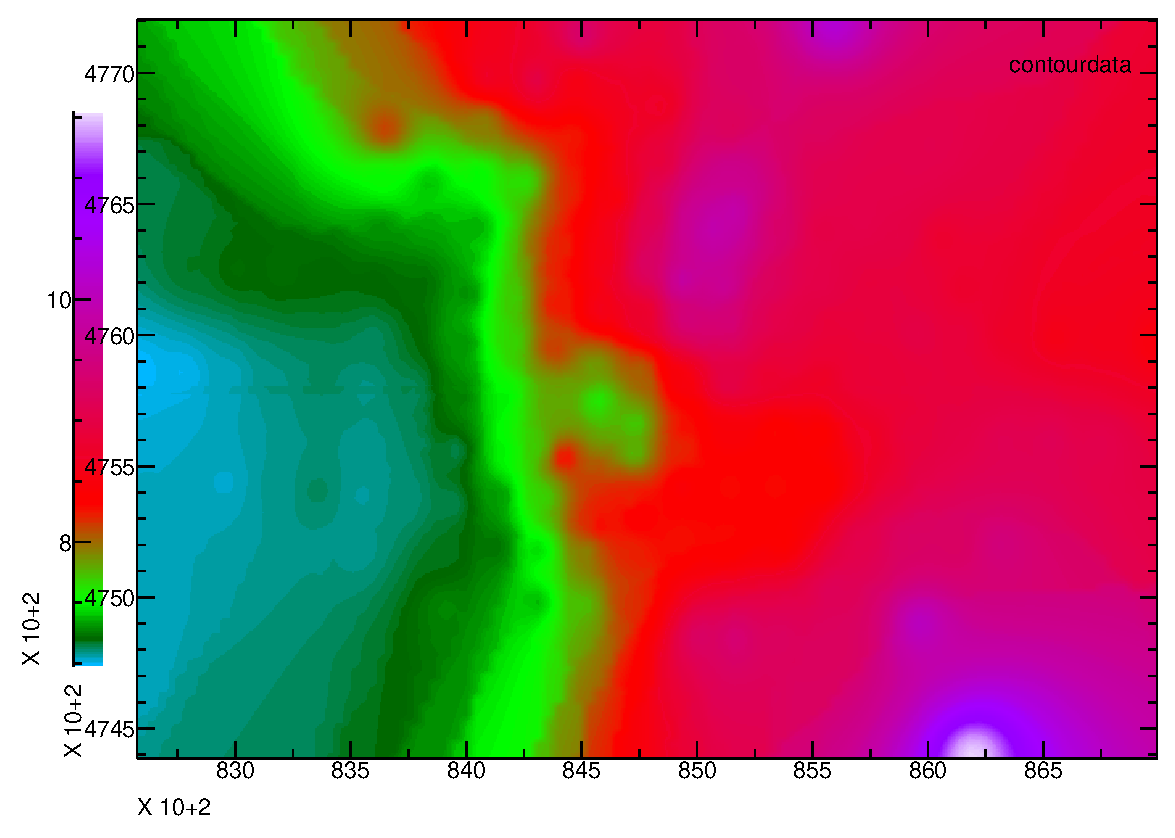
\includegraphics[width=0.9\textwidth]{image}
\caption{image示意图}
\end{figure}

\SACTitle{头段变量}
需要: iftype (设为``IXYZ''), nxsize, nysize

使用:xminimum, xmaximum, yminimum, ymaximum

\SACCMD{inicm}
\label{cmd:inicm}

\SACTitle{概要}
重新初始化SAC

\SACTitle{语法}
\begin{SACSTX}
INICM
\end{SACSTX}

\SACTitle{说明}
这个命令可以在任意时刻将SAC初始化到其刚启动的状态。所有活动的图像设备被终止,
全局变量初始化到其初始值,内存中数据丢失。

\SACCMD{installmacro}
\label{cmd:installmacro}

\SACTitle{概要}
将一个宏文件安装到SAC全局宏目录中

\SACTitle{语法}
\begin{SACSTX}
INSTALLMACRO name [name ...]
\end{SACSTX}

\SACTitle{输入}
\begin{itemize}
\item name SAC宏文件名
\end{itemize}

\SACTitle{说明}
这个命令让你将你自己的宏文件安装到全局宏目录中,这样所有人都可以使用,全局宏目录位于
~\lstinline{sac/aux/macros}~。

\SACTitle{相关命令}
\nameref{cmd:macro}

\SACCMD{int}
\label{cmd:int}

\SACTitle{概要}
利用梯形或矩形方法对数据进行积分

\SACTitle{语法}
\begin{SACSTX}
INT T!RAPEZEIDAL!|R!ECTANGULAR!
\end{SACSTX}

\SACTitle{缺省值}
\begin{SACDFT}
INT TRAPEZOIDAL
\end{SACDFT}

\SACTitle{说明}
这个命令使用梯形或矩形方式对数据积分,输出的第一个数据点值为0,如果使用梯形积分,数据点数将少一个,数据不必等间隔

\SACTitle{错误消息}
\begin{itemize}
\item[-]1301: 未读入文件
\item[-]1307: 对谱文件非法操作
\end{itemize}

\SACTitle{头段变量改变}
depmin, depmax, depmin

\SACCMD{interpolate}
\label{cmd:interpolate}

\SACTitle{概要}
插值等间距或不等间距文件,获得新采样率

\SACTitle{语法}
\begin{SACSTX}
INTERP!OLCATE! [D!ELTA! v] [E!PSILON! v] [B!EGIN! v|OFF] [N!PTS! n|OFF]
\end{SACSTX}

\SACTitle{输入}
\begin{itemize}
\item DELTA v: 设置新采样率为v.
\item EPSILON v: 设置内插收敛因子为v
\item BEGIN v :  在v处开始内插,这个值作为内插生成文件的起始值 
\item BEGIN OFF : 在未插值数据的起始时间开始插值 
\item NPTS n : 强制插值后文件数据点为n 
\item NPTS OFF : 由SAC根据起始、结束时间以及新采样率自动计算插值后的数据点数. 
\end{itemize}

\SACTitle{缺省值}
\begin{SACDFT}
interpolate delta 0.025 epsilon 0.0001 begin off npts off
\end{SACDFT}

\SACTitle{说明}
这个命令使用Wiggins内插方法将不等间距数据转换为等间距数据并重采样等间距数据得到新的采样率

\SACTitle{例子}
假设文件filea是不等间距文件,为了将其转换为采样率为0.01s的等间距文件:
\begin{SACCode}
SAC> read filea
SAC> interpolate delta 0.01
\end{SACCode}

假设文件fileb是采样率为0.025s的等间隔文件,将其转换为采样率为0.02s:
\begin{SACCode}
SAC> read fileb
SAC> interpolate delta 0.02
\end{SACCode}

假设你想强制插值后文件采样率为0.005,起始时间为18.237,有400个点:
\begin{SACCode}
SAC> read filec
SAC> interpolate delta 0.005 begin 18.237 npts 400
\end{SACCode}

\SACTitle{警告消息}
\begin{itemize}
\item[-]2008: 要求的开始时间小于文件起始时间。
\item[-]2009: 要求的结束时间大于文件结束时间
\end{itemize}

\SACTitle{参考文献}
Wiggins, 1976, BSSA, 66, p.2077.

\SACTitle{头段变量改变}
delta, npts, e

\SACCMD{keepam}
\label{cmd:keepam}

\SACTitle{概要}
保留SAC内存中谱文件的振幅部分(谱文件可以是AMPH或RLIM格式)

\SACTitle{语法}
\begin{SACSTX}
KEEPAM
\end{SACSTX}

\SACTitle{说明}
这个命令使得用户可以很容易的丢弃相位部分,以便对幅度部分进行一维数组的代数运	算操作。如果文件是RLIM格式,则数据在丢弃相位之前首先转换为AMPH格式,最后得到的结果文件中的振幅分量数据为一般xy文件,因此其可以与时间域文件区分开。

\SACCMD{khronhite}
\label{cmd:khronhite}

\SACTitle{概要}
对数据应用Khronhite滤波器

\SACTitle{语法}
\begin{SACSTX}
KHRONHITE [v]
\end{SACSTX}

\SACTitle{输入}
\begin{itemize}
\item v : 截断频率,单位Hz
\end{itemize}

\SACTitle{缺省值}
\begin{SACDFT}
KHRONHITE 2.0
\end{SACDFT}

\SACTitle{说明}
这个低通滤波器是带有串取二级四阶Butterworth低通滤波器的模拟滤波器的数值逼近。其拐角频率为0.1Hz以加强区域范围内基谐瑞利波(Rg)的振幅信号。

\SACTitle{头段变量改变}
depmin, depmax, depmen

\SACCMD{line}
\label{cmd:line}

\SACTitle{概要}
控制绘图中线型的选择

\SACTitle{语法}
\begin{SACSTX}
LINE [ON|OFF|S!OLID!|D!OTTED!|n] [I!NCREMENT! [ON|OFF]] [L!IST! STANDARD|NLIST]
\end{SACSTX}

\SACTitle{输入}
\begin{itemize}
\item ON : 打开线型选项,不改变线型 
\item OFF : 关闭线型开关 
\item SOLID : 改变线型为实线型,并打开线型开关 
\item DOTTED : 改变线型为虚线型,并打开线型开关 
\item n : 将线型设置为n并打开线型开关。线型为0代表关闭线型开关。线型的编号随设备变化 
\item INCREMENT {ON} : 每个数据被绘出之后,按照线型表中的次序改变为另一个线型 
\item INCREMENT OFF : 不改变线型 
\item LIST nlist : 改变线型列表的目录,输入线型编号的列表 
\item LIST STANDARD : 设置为标准线型列表 
\end{itemize}

\SACTitle{缺省值}
\begin{SACDFT}
line solid increment off list standard
\end{SACDFT}

\SACTitle{说明}
这个命令控制绘图时的线型,图形的框架(轴、标题等等)通常使用实线。网格的线型用GRID命令控制。并非所有的图形设备都有除实线型之外的其他线型的,在那些设备上显然这个命令没有什么效果。而对于不同的设备线型号n也可能是不同的。

还有其他命令可以控制数据显示的其他方面。SYMBOL命令用于将每个数据点的值用一个符号显示在图上。

COLOR命令控制彩色图形设备的颜色选择。所有的这些属性都是独立的。如果你想的话你可以选择在每个数据点上选择带符号的蓝色虚线。线型为0代表关闭画线选项。在LIST选项和SYMBOL命令中可以利用线型为0的特性,在同一张图上将某些数据用线显示某些数据用符号显示

\SACTitle{例子}
选择依次变化的线型,从线型1开始:
\begin{SACCode}
SAC> line 1 increment
\end{SACCode}

改变线型表使之包含线型3, 5 和 1:
\begin{SACCode}
SAC> line list 3 5 1
\end{SACCode}

使用PLOT2在同一个图形上绘制三个文件,第一个使用实线无符号,第二个没有线条,用三角符号,第三个无线条,用十字符号:
\begin{SACCode}
SAC> read file1 file2 file3
SAC> line list 1 0 0 increment
SAC> symbol list 0 3 7 increment
SAC> plot2
\end{SACCode}

\SACTitle{相关命令}
\nameref{cmd:symbol}、\nameref{cmd:color}

\SACCMD{linefit}
\label{cmd:linefit}

\SACTitle{概要}
计算内存中数据的线性拟合,结果写到暂存块变量中

\SACTitle{语法}
LINEFIT

\SACTitle{说明}
对数据计算最小平方拟合得到一条直线,斜率以及y轴截距,斜率的标准差,截距的标准差,数据的标准差以及数据之间的互相关系数将分别被写入暂存块变量SLOPE,YINT,SDSLOPE,SDYINT,SDDATA以及CORRCOEF。数据不必是等间隔文件。

\SACTitle{错误消息}
\begin{itemize}
\item[-]1301: 未读入数据文件
\item[-]1307: 对谱文件的非法操作
\end{itemize}

\SACTitle{最近修订}
September 12, 1995 (Version 00.38)

\SACCMD{linlin}
\label{cmd:linlin}

\SACTitle{概要}
设置X、Y轴均为线性

\SACTitle{语法}
\begin{SACSTX}
LINLIN
\end{SACSTX}

\SACTitle{相关命令}
\nameref{cmd:linlog}、\nameref{cmd:loglog}、\nameref{cmd:loglin}

\SACCMD{linlog}
\label{cmd:linlog}

\SACTitle{概要}
设置X轴为线性,Y轴均为对数坐标

\SACTitle{语法}
\begin{SACSTX}
LINLOG
\end{SACSTX}

\SACTitle{相关命令}
\nameref{cmd:linlin}、\nameref{cmd:loglog}、\nameref{cmd:loglin}

\SACCMD{listhdr}
\label{cmd:listhdr}

\SACTitle{概要}
列出被选择的头段变量的值

\SACTitle{语法}
\begin{SACSTX}
L!ist!H!dr! [D!efault!|P!icks!|SP!ecial!] [FILES ALL|NONE|list] [COLUMNS 1|2] 
    [INCLUSIVE ON|OFF] [hdrlist]
\end{SACSTX}

\SACTitle{输入}
\begin{itemize}
\item DEFAULT : 使用默认的头段列表,它列出了所有定义了的头段变量。
\item PICKS : 使用picks列表,包含了用于定义时间拾取的头段 
\item SPECIAL :  使用用户定义的特别列表 
\item FILES ALL : 列出内存中所有文件的头段 
\item FILES NONE : 不列出头段,为将来的命令设置默认值 
\item FILES list : 列出部分文件的头段,list是要处理的文件号 
\item COLUMNS 1 : 每行一列的输出格式  
\item COLUMNS 2 : 每行两列的输出格式  
\item INCLUSIVE :  ON表示包含没有定义的头段变量,OFF则不包含 
\item hdrlist : 要列出的头段列表  
\end{itemize}

\SACTitle{缺省值}
\begin{SACDFT}
LISTHDR DEFAULT FILES ALL COLUMNS 1 INCLUSIVE OFF
\end{SACDFT}

\SACTitle{说明}
用户可以自己定义要列出的项或使用标准列表中的任一个,DEFAULT列表包含全部头段变量。PICKS列表包含直接或间接用于定义时间拾取的头段变量,这个列表包含B, E,O, A, Tn, KZTIME, KZDATE。用户自己可以随时定义一个特殊列表而且可以通过SPECIAL选项再次使用。命令输出列表包含头段变量名,等于号以及当前值。有些头段可能未定义。SAC在这些未定义的头段中储存一个特别的标志以标记它们,对于整数和浮点数未定义值为-12345,字符串以及那些用于表示字符串含义的整数未定义值为``UNDEFINED''.

\SACTitle{错误消息}
\begin{itemize}
\item[-]1301: 未读入文件
\end{itemize}

\SACTitle{例子}
获取picks列表,输出为两列显示:
\begin{SACCode}
SAC> lh picks column 2
\end{SACCode}

获得第三、四个文件的默认头段列表:
\begin{SACCode}
SAC> lh files 3 4
\end{SACCode}

列出文件开始和结束时间:
\begin{SACCode}
SAC> lh b e
\end{SACCode}

定义一个包含台站参数的特殊列表:
\begin{SACCode}
SAC> lh KSTNM STLA STLO STEL STDP
\end{SACCode}

稍后再次使用上面的特殊列表:
\begin{SACCode}
SAC> lh SPECIAL
\end{SACCode}

只是设置默认两列输出:
\begin{SACCode}
SAC> lh COLUMNS 2 FILES NONE
\end{SACCode}

\SACCMD{load}
\label{cmd:load}

\SACTitle{概要}
导入外部命令(在SAC的linux版本中外部命令的导入需要额外的工作)

\SACTitle{语法}
\begin{SACSTX}
LOAD comname [ABBREV abbrevname]
\end{SACSTX}

\SACTitle{输入}
\begin{description}
\item [comname] 从一个共享目标文件中载入的一个外部函数名 
\item [ABBREV abbrevname] 命令的简写 
\end{description}

\SACTitle{说明}
这个命令允许用户载入由SAC外部命令接口写的命令。(参见EXTERNAL\_INTERFACE文档)。这个命令必须是一个储存在共享目标库(.so文件)中。SAC将检查所有环境变量SACSOLIST中的共享目标库,这个环境变量需要包含一个或多个共享目标库,每个库以空格分割。到这些共享目标库的路径必须在环境变量LD\_LIBRARY\_PATH中指定。如果SACSOLIST为设置,则SAC将使用由LD\_LIBRARY\_PATH中指定的路径在共享文件库libsac.so中寻找。一个叫做libcom.so的库随着SAC发布。

\SACTitle{示例}
设置你的环境变量使得SAC在当前目录从库文件libbar.so中查找一个称为foo的命令,并为foo设置别名为myfft:
\begin{SACCode}
% export SACSOLIST = "libcom.so libbar.so"
#  Add the current directory to the search path.
% export LD_LIBRARY_PATH {$LD_LIBRARY_PATH}:. 
% sac
SAC> load foo abbrev myfft* load the command
SAC> read file1.z file2.z file3.z  * input files to pass to the command
SAC> myfft real-imag* invoke command with its arguments,
* commands must parse their own args.
SAC> psp
\end{SACCode}

如何创建一个包含你的命令的共享目标库:
\begin{SACCode}
Solaris::
cc -o libxxx.so -G extern.c foo.c bar.c
SGI::
cc -g -o libxxx.so -shared foo.c bar.c
LINUX: (gcc)::
gcc -o libxxx.so -shared extern.c foo.c bar.c sac.a
\end{SACCode}
其中sac.a可以从你得到sac的地方获得

\SACTitle{SAC发布的外部命令}
在SAC的发布版中有一个外部命令,叫做FLIPXY。FLIPXY将一个或多个X-Y数据文件作为输入,并调换X和Y。这个命令在SAC/aux/external中的libcom.so中,同时还有FLIPXY的源代码作为参考。为了导入FLIPXY,libcom.so必须包含在SACSOLIST中

\SACTitle{错误消息}
\begin{itemize}
\item[-]1028: 外部命令不存在:这意味着SAC无法找到你的外部命令
\end{itemize}

这个错误产生的原因很多,一个可能是环境变量LD\_LIBRARY\_PATH不包含到达你的共享库的目录。
另一个可能的原因是SACSOLIST不包含你的共享库的名字

\SACCMD{loadctable}
\label{cmd:loadctable}

\SACTitle{概要}
允许用户在彩色绘图中选择一个新的颜色表

\SACTitle{语法}
LoadCTable n | [ DIR CURRENT | name ] [ filelist ]

\SACTitle{输入}
\begin{itemize}
\item n : 标准SAC颜色表对于的号,n可以取1-17
\item DIR CURRENT : 从当前目录载入颜色表,当前目录指的是你启动SAC的目录
\item DIR name : 从目录name中载入颜色表,这是一个相对或绝对目录名 
\item filelist : 颜色表文件列表 
\item file : 一个合法的颜色表文件名,其可以是简单文件名或或者一个路径名,这个路径可以是相对路径或绝对路径 
\end{itemize}

\SACTitle{说明}
这个命令允许用户选择一个新的颜色表或者通过指定颜色表的文件以及路径提供他们自己的颜色表。
如果未使用DIR选项,SAC将首先在SACAUX中寻找颜色表,然后在用户的工作目录中寻找.

*在SACAUX下可以的ctables下有21个文件,其中一个为gmt.cpt,用于在SAC中绘制与GMT有关的彩色图形,另外20个文件为三列数据,应该就是颜色表了,前面说的n取1到17可能有些过时了。具体谁对应谁还不清楚,just try them!

\SACTitle{最近修订}
May 26, 1995 (Version 00.31)

\SACCMD{log}
\label{cmd:log}

\SACTitle{概要}
对每个数据点做自然对数

\SACTitle{语法}
\begin{SACSTX}
LOG
\end{SACSTX}

\SACTitle{错误消息}
\begin{itemize}
\item[-]1301: 未读入文件
\item[-]1307: 对谱文件非法操作
\item[-]1340: 文件中数据点值超出允许的范围(对数要求值为正)
\end{itemize}

\SACTitle{头段变量改变}
depmin, depmax, depmen

\SACCMD{log10}
\label{cmd:log10}

\SACTitle{概要}
对每个数据点取以10为底对数($\log_{10} y$)

\SACTitle{语法}
\begin{SACSTX}
LOG10
\end{SACSTX}

\SACTitle{错误消息}
\begin{itemize}
\item[-]1301: 未读入文件
\item[-]1307: 对谱文件的非法操作
\item[-]1340: 文件中数据值超出允许的范围(要求所有数据值均为正)
\end{itemize}

\SACTitle{头段变量}
depmin、depmax、depmen

\SACCMD{loglab}
\label{cmd:loglab}

\SACTitle{概要}
控制对数轴的标签

\SACTitle{语法}
LOGLAB [ ON | OFF ]

\SACTitle{输入}
\begin{itemize}
\item ON : 打开对数标签开关 
\item OFF : 关闭对数标签开关 
\end{itemize}

\SACTitle{缺省值}
LOGLAB ON

\SACTitle{说明}
标签一般位于轴上每个10的对数值处,如果这个选项被打开并且标签之间有足够的空间的话在整数对数值中间将加入第二标签。

\SACTitle{最近修订}
January 8, 1983 (Version 8.0)

\SACCMD{loglin}
\label{cmd:loglin}

\SACTitle{概要}
设置X轴为对数坐标、Y轴为线性

\SACTitle{语法}
LOGLIN

\SACTitle{相关命令}
LINLOG, LOGLOG, LINLIN

\SACTitle{最近修定}
January 8, 1983 (Version 8.0)

\SACCMD{loglog}
\label{cmd:loglog}

\SACTitle{概要}
设置X、Y轴均为对数坐标

\SACTitle{语法}
\begin{SACSTX}
LOGLOG
\end{SACSTX}

\SACTitle{相关命令}
\nameref{cmd:linlog}、\nameref{cmd:linlin}、\nameref{cmd:loglin}

\section{lowpass}
\label{cmd:lowpass}

\SACTitle{概要}
对数据文件应用一个无限脉冲高通滤波器

\SACTitle{语法}
LowPass [ BUtter | BEssel | C1 | C2 ] [ Corners v1 v2 ] [ Npoles n ] [ Passes n ] [ Tranbw v ] [ Atten v ]

\SACTitle{输入}
\begin{itemize}
\item BUtter: 应用一个Butterworth滤波器
\item BEssel: 应用一个Bessel滤波器
\item C1: 应用一个Chebyshev I型滤波器
\item C2: 应用一个Chebyshev II滤波器
\item Corners v1 v2: 设定拐角频率分别为v1和v2,即频率通带为v1-v2
\item Npoles n: 设置极数为N,范围: 1-10
\item Passes n: 设通道数为N,范围: 1-2
\item Tranbw v: 设置Chebyshev转换带宽为v
\item Atten v: 设置Chebyshev衰减因子为v
\end{itemize}

\SACTitle{缺省值}
LOWPASS BUTTER CORNER 0.2 NPOLES 2 PASSES 1 TRANBW 0.3 ATTEN 30

\SACTitle{说明}
参见BANDPASS

\SACTitle{例子}
为应用一个四极Butterworth,拐角频率为2Hz.:
\begin{SACCode}
SAC> lp n 4 c 2
\end{SACCode}
在此之后如果要应用一个二极双通具有相同频率的Bessel:
\begin{SACCode}
SAC> lp n 2 be p 2
\end{SACCode}

\SACTitle{错误消息}
\begin{itemize}
\item[-]1301: 未读入文件
\item[-]1306: 对不等间隔文件的非法操作
\item[-]1307: 对谱文件的非法操作
\item[-]1002: 由于拐角频率大于Nyquist频率而出现的坏值
\end{itemize}

\SACTitle{头段变量改变}
DEPMIN, DEPMAX, DEPMEN

\SACTitle{最近修订}
January 8, 1983 (Version 8.0)

\SACCMD{macro}
\label{cmd:macro}

\SACTitle{概要}
执行SAC宏文件

\SACTitle{语法}
Macro name [ arguments ]

\SACTitle{输入}
\begin{itemize}
\item name : 要执行的SAC宏文件名
\item arguments : 宏文件参数
\end{itemize}

\SACTitle{说明}
关于SAC宏文件的详细信息请参考相关文档。宏文件可以在当前目录,也可以在用SETMACRO预先指定的目录,或者在SAC的全局宏目录sac/aux/macros下。

\SACTitle{相关命令}
SETMACRO, INSTALLMACRO

\SACTitle{最近修订}
May 15, 1987 (Version 10.2)

\SACCMD{map}
\label{cmd:map}

\SACTitle{概要}
利用SAC内存中的所有数据文件生成一个包含台站/事件符号、地形以及台站名的
GMT地图,也可以在命令行上指定一个事件文件。每个
地震事件符号可以根据震级、残差等确定其大小。这个命令会产生一个ps文件,
并将该文件在屏幕上显示,同时产生一个绘制该图的shell脚本。

\SACTitle{语法}
MAP\quad [ MERcator | EQuidistant | AZimuthal\_equidistant | ROBinson ] [ WEST minlon ] [ EAST maxlon ] [ NORTH maxlat ] [ SOUTH minlat ] [ MAGnitude | REsidual | RMean\_residual ] [ EVentfile filename ] [ TOPOgraphy ] [ STANames ] [MAPSCALE on | off ] [ PLOTSTATIONS on | off ] [ PLOTEVENTS on | off ] [ PLOTLEGEND on | off ] [ LEGENDXY x y ] [ FILE output-file ]

\SACTitle{输入}
SAC中可以使用的投影方式包括:
\begin{itemize}
\item MERCATOR:	投影方式为Mercator投影。
\item EQUIDISTANT: 投影方式为等间距圆柱投影,经纬度为线性。
\item ROBINSON: 投影方式为Robinson投影,适用于世界地图。
\item LAMBERT: 适用于东西范围较大的区域。
\item UTM:通用横向Mercator(尚未实现)。
\end{itemize}

下面的选项允许用户指定地图的区域,其默认使用台站以及事件经纬度的最小最大值(如果真是如此,这样的缺省值并不合适,因为那样意味着某些台站或事件将位于地图的边界处,但是实际上地图范围给的还是不错的):
\begin{itemize}
\item WEST :  地图的最小经度 
\item EAST : 地图的最大经度 
\item NORTH : 地图的最大纬度 
\item SOUTH : 地图的最小纬度 
\item AUTOLIMITS:  自动决定地图的区域 [缺省值] 
\end{itemize}
  
下面的选项允许用户向地图中添加位置和注释:
\begin{itemize}
\item STANames on | off :  在地图上绘制台站名[默认为off]
\item MAPSCALE on | off :  在地图上绘制地图比例尺[默认为off]
\item PLOTSTATIONS on | off : 绘制地震图给出的全部台站[默认为on]
\item PLOTEVENTS on | off : 绘制eventfile和/或地震图给出的全部事件[默认为on]
\end{itemize}

下面的选项允许用户根据不同的值给出不同地震事件符号的大小。默认值是所有符号大小一样:
\begin{itemize}
\item MAGnitude : user0定义地震震级,user0越大,则事件符号越大。
\item REsidual : user0定义残差。根据user0的绝对值定义事件符号的大小。正值为(+) 负值为(-).
\item RMean\_residual : 与residual相同,除了将所有残差去除均值之外
\item PLTLEGEND on | off : 绘制地震震级以及残差的图例[默认为on] 
\item LEGENDXY x y : 绘制图例的绝对位置,默认为[1,1]。位置是相对于页面的左下角,其单位为inch。 这是一个与地震震级和残差有关的图例。
\item EVENTFILE : 指定一个自由格式的ASCII文本文件,其包含了额外的事件数据,文件的每一行包含单个事件的数据。每行的头两列必须包含纬度和经度(单位为度)。第三列可以包含符号大小信息(比如震级、深度、走时残差等)。
\item TOPOgraphy on | off : 设置TOPO为开允许用户向地图中添加地形和海洋深度。这个命令读取GMT中grdraster.info的第一个地形文件,当然地形文件中必须要有该区域的数据。地形彩色图使用\$SACAUX/ctables/gmt.cpt。网格文件被写入当前目录
\item FILE : 默认的输出文件名为gmt.ps,你可以通过FILE选项指定文件名
\end{itemize}
可以用SAC的TITLE命令指定其标题

\SACTitle{缺省值}
   MAP MERCATOR TOPO off STAN off FILE gmt.ps PLOTSTATIONS on PLOTEVENTS on

\SACTitle{例子}
利用SAC提供的一些数据作为例子:
\begin{SACCode}
SAC> r /opt/sac/aux/datagen/regional/*.z
SAC> map stan on 
Using Default Postscript Viewer
	gs -sDEVICE=x11 -q -dNOPROMPT -dTTYPAUSE 
	Set an alternative through the SACPSVIEWER environment variable
	Press any key to continue
\end{SACCode}
绘制出的地图如图\ref{fig:map}所示,整个地图的边界控制的还算不错,还算比较美观,
三角形代表台站位置,圆形代表地震位置,大小也控制的不错。生成这个图的同时,还有
一个可以用于生成该地图的shell脚本。
\begin{SACCode}
#!/bin/csh -f

# Set the output file
set psfile = "./gmt.ps"

# Start the Postscript file 
psbasemap -JM6.5i -R-120.572/-110.404/33.754/41.380 \
-Ba3.000f3.000/a2.000f2.000NEWS:."": -X0.75i -Y1.0i -P -K > $psfile 

# Add the Coastline and National Boundaries
pscoast -K -O -J -R -B -N1 -N2 -W -Dl -A78 -G250/250/200  >> $psfile 

# Add station location labels.  
# Input are longitude, latitude, and name.
pstext -K -O -D0.10i/0.10i -J  -R -S0.25/255 -G0/0/0 <<EOF >> $psfile 
-115.239 40.745  10 0 0 BL  ELK      
-112.822 37.017  10 0 0 BL  KNB      
-116.411 34.390  10 0 0 BL  LAC      
-118.154 38.432  10 0 0 BL  MNV      
EOF

# Add station locations.  
# Input are longitude latitude.
psxy -K -O -J -R -St0.25i -G0/0/0 <<EOF >> $psfile 
-115.239 40.745 
-112.822 37.017 
-116.411 34.390 
-118.154 38.432 
EOF

# Add event locations.
# Input are longitude latitude.
psxy -O -K -J -R -W10/0/0/0  -Sc0.25i  <<EOF >> $psfile 
-118.123 37.852 
EOF

# End the Postscript File
psxy -R -J -O /dev/null >> $psfile 
\end{SACCode}

\begin{figure}[h]
\centering
\caption{map例子示意图}
\label{fig:map}
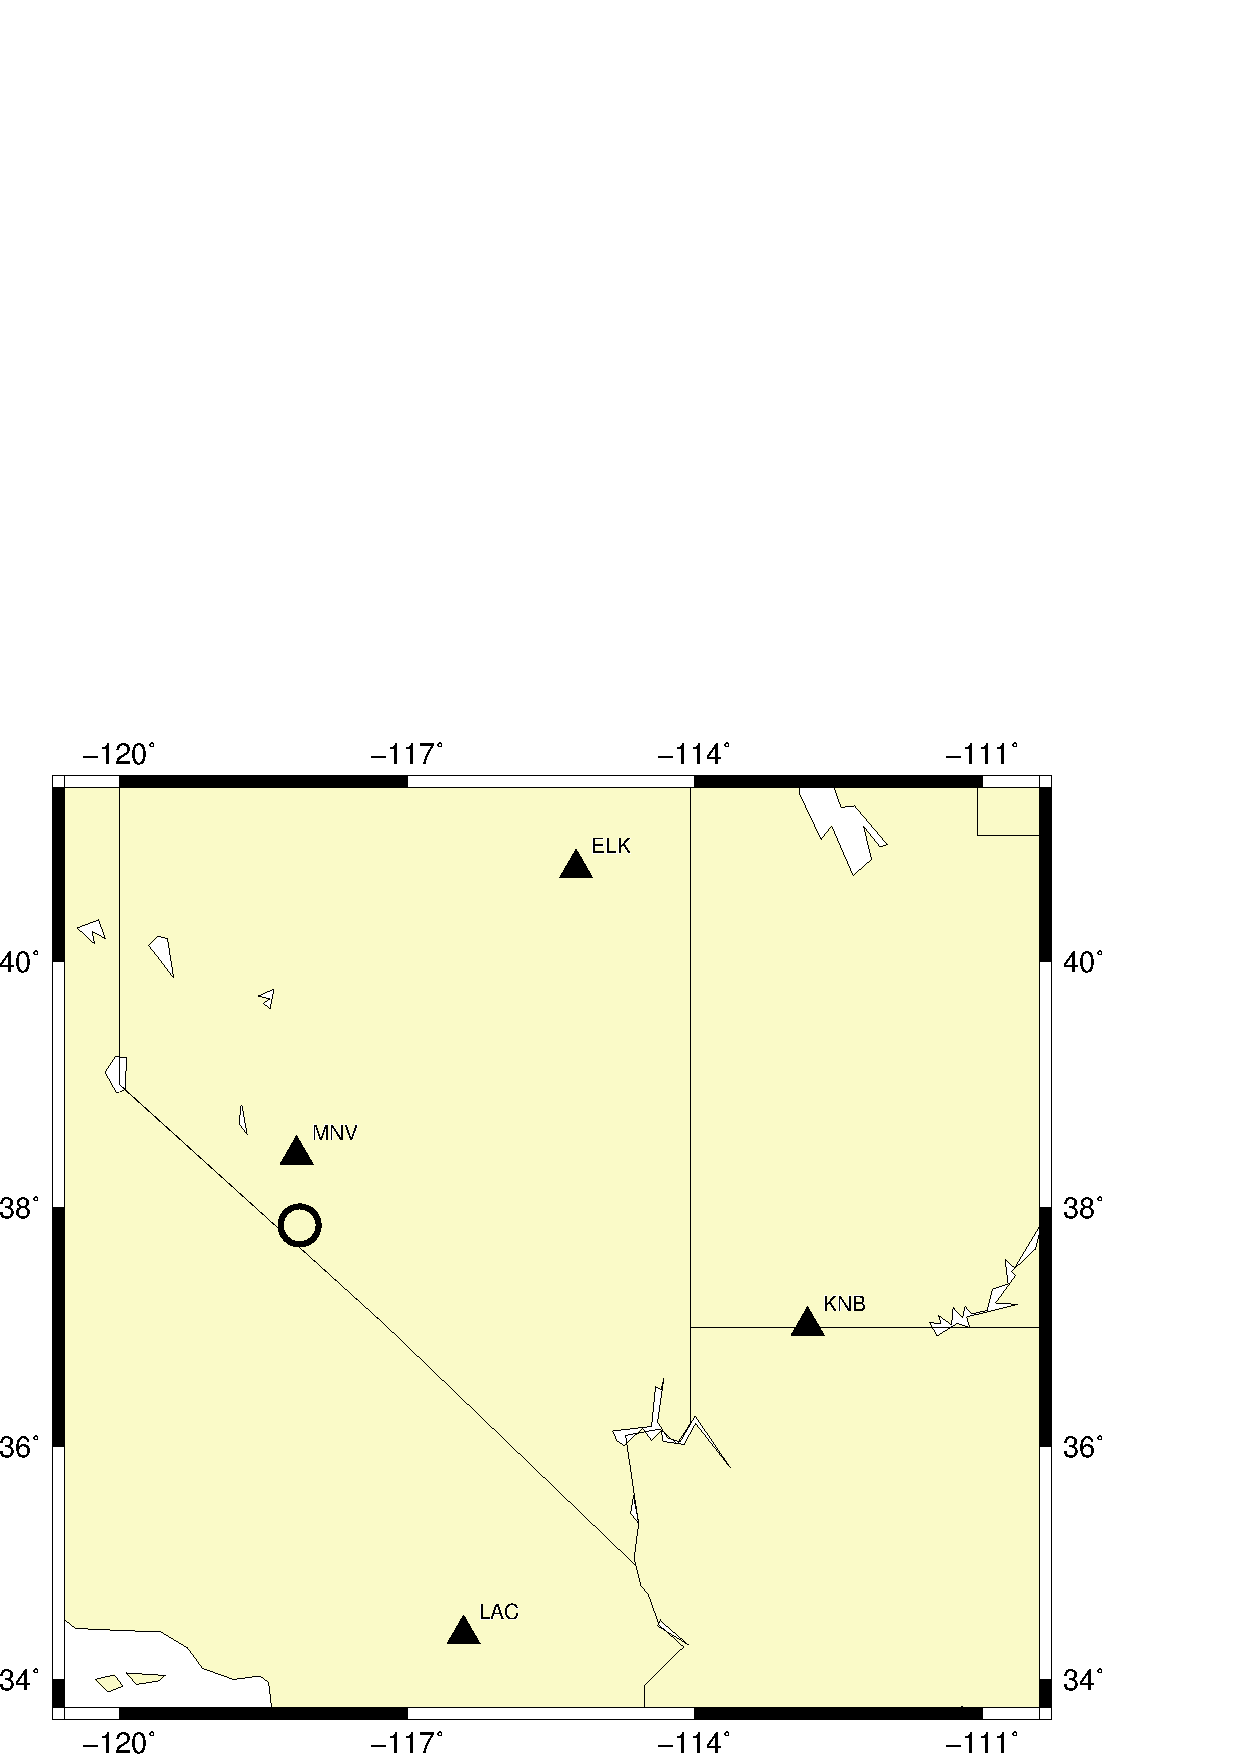
\includegraphics[width=10cm]{map}
\end{figure}

\SACTitle{头段数据}
台站纬度(stla)以及经度(stlo)必须在头段中被定义。如果事件纬度(evla)以及经度(evlo)被定义则其会被包含在地图中。如果这个命令在执行BBFK之后执行,MAP将沿着反方位角方向绘制大圆弧路径。
这个版本的MAP是基于4.0版本的Generic Mapping Tools,要执行这个命令,你需要将GMT4.0安装在你的机器上并保证可执行文件位于路径中。

每个MAP命令的结果将写入当前目录下一个称为gmt.csh的脚本中。用户可以修改这个文件以利用更多SAC未利用的选项。默认单位是inch,当然可以在脚本中修改。

在使用pscoast绘制海岸线时,SAC采用了-Dl选项,其中l代表低精度的海岸线数据。用户
可以在脚本中修改使用更高精度的海岸线数据。

该脚本采用的shell是csh,其很容易改成bash脚本。

MAP命令的结果将自动被显示。用于显示的默认程序是gs(ghostscript)。用户可以通过设置环境变量SACPSVIEWER选择其他显示工具。\\
在csh下可以这样设置:
\begin{SACCode}
setenv SACPSVIEWER "gs -sDEVICE=x11 -q -dNOPROMPT -dTTYPAUSE"
\end{SACCode}
在bash下可以这样设置:
\begin{SACCode}
export SACPSVIEWER="gs -sDEVICE=x11 -q -dNOPROMPT -dTTYPAUSE"
\end{SACCode}

\SACCMD{markptp}
\label{cmd:markptp}

\SACTitle{概要}
在测量时间窗内测量并标记最大峰峰值

\SACTitle{语法}
MARKPtp [ Length v ] [ To marker ]

\SACTitle{输入}
\begin{itemize}
\item LENGTH v : 设置滑动窗的长度为v秒 
\item TO marker : 定义头段中用于储存结果的第一个时间标记。最小值的时间记录在这个时间标记中,最大值的时间标记储存在下一个时间标记中。 
\item marker : Tn(n=0-9)
\end{itemize}

\SACTitle{缺省值}
MARKPTP LENGTH 5.0 TO T0

\SACTitle{说明}
这个命令测量数据在当前测量时间窗内最大峰峰值对应的时间和幅度。结果写入头段变量中。波谷对应的时间写入命令给出的时间标记中,波峰对应的时间写入下一个命令标记。峰峰值写入USER0中,这个结果也可以通过OAFP命令写入字符数字型震相拾取文件。

\SACTitle{例子}
设置测量时间窗为头段T4和T5之间,并使用默认的滑动时间窗长和标记:
\begin{SACCode}
SAC> MTW T4 T5
SAC> MARKPTP
\end{SACCode}

设置测量时间窗为初动之后的30s,滑动时间窗为3s,起始时间标记为T7:
\begin{SACCode}
SAC> MTW A 0 30
SAC> MARKP L 3. TO T7
\end{SACCode}

\SACTitle{头段变量改变}
Tn, USER0, KTn, KUSER0

\SACTitle{相关命令}
MTW , OAPF

\SACTitle{最近修订}
May 15, 1987 (Version 10.2)

\SACCMD{marktimes}
\label{cmd:marktimes}

\SACTitle{概要}
根据一个速度集得到走时并对数据文件进行标记

\SACTitle{语法}
\begin{SACSTX}
MARKT!IMES! [T!O! marker] [D!ISTANCE! H!EADER!|v] [O!RIGIN! H!EADER!|v|GMT time] 
    [V!ELOCITIES! v ... ]
\end{SACSTX}

\SACTitle{输入}
\begin{itemize}
\item TO marker : 定义头段中用于储存结果的第一个时间标记。对下一个的速度使用下一个时间 
\item marker :  T0|T1|T2|T3|T4|T5|T6|T7|T8|T9 
\item DISTANCE HEADER : 使用头段中的DIST代表距离用于走时计算 
\item DISTANCE v : 使用v作为走时计算中的距离 
\item ORIGIN HEADER : 使用头段中的参考时间(O)用于走时计算 
\item ORIGIN v : 使用相对参考时间偏移v秒用于走时计算 
\item ORIGIN GMT time : 使用Greenwich平均时间作为参考时间 
\item time :  GMT时间包含六个整数:年、儒略日、时、分、秒、毫秒 
\item VELOCITIES v ... : 设置用于走时计算的速度集,最多可以输入10个速度 
\end{itemize}

\SACTitle{缺省值}
\begin{SACDFT}
marktimes velocities 2. 3. 4. 5. 6.  distance header origin header to t0
\end{SACDFT}

\SACTitle{说明}
这个命令在头段中标记震相的到时,给定事件的发生时间,震中距以及速度即可计算到	时。下面的方程用于简单估计走时:
 		\[ time(j) = origin + \frac{distance}{velocity(j)} \]
结果被写入指定的时间标记中

\SACTitle{例子}
使用默认的速度集,强制距离为340km,第一个时间标记为T4:
\begin{SACCode}
SAC> marktimes distance 340. to t4
\end{SACCode}

选择一个不同的速度集:
\begin{SACCode}
SAC> markt v 3.5 4.0 4.5 5.0 5.5
\end{SACCode}

设置新的参考时间并将结果保存在T2中:
\begin{SACCode}
SAC> markt origin gmt 1984 231 12 43 17 237 to t2
\end{SACCode}

\SACTitle{头段变量改变}
Tn, KTn

\SACCMD{markvalue}
\label{cmd:markvalue}

\SACTitle{概要}
在数据文件中搜索并标记某个值

\SACTitle{语法}
\begin{SACSTX}
MARKV!ALUE! [GE|LE v] [TO marker]
\end{SACSTX}

\SACTitle{输入}
\begin{description}
\item [GE v] 搜索并标记第一个大于或等于v的数据点 
\item [LE v] 搜索并标记第一个小于或等于v的数据点 
\item [TO marker] 定义头段中储存结果的时间标记 
\item [marker] T0|T1|T2|T3|T4|T5|T6|T7|T8|T9 
\end{description}

\SACTitle{缺省值}
\begin{SACDFT}
markvalue ge 1 to t0
\end{SACDFT}

\SACTitle{说明}
这个命令在每一个数据文件中搜索,满足要求的值并将第一次出现该值的时间标记下来,
如果测量时间窗已经被定义(参见MTW),则只有那部分的文件才会被搜索。
否则将搜索整个文件,结构写入头段中的时间标记中

\SACTitle{示例}
搜索文件中第一个值大于3.4的点并将结果保存在头段T7中:
\begin{SACCode}
SAC> markvalue ge 3.4 to t7
\end{SACCode}

稍后在以T4起始的10s测量时间窗中使用相同的搜索:
\begin{SACCode}
SAC> mtw t4 0 10
SAC> markvalue
\end{SACCode}

\SACTitle{头段变量改变}
Tn, KTn

\SACTitle{相关命令}
\nameref{cmd:mtw}

\SACCMD{merge}
\label{cmd:merge}

\SACTitle{概要}
将一系列文件合并(首位相连)内存中的数据中

\SACTitle{语法}
MERGE [ COMMIT|ROLLBACK|RECALLTRACE] [ filelist ]

\SACTitle{输入}
\begin{itemize}
\item COMMIT|ROLLBACK|RECALLTRACE 参见专门的说明
\item filelist: SAC二进制数据文件列表
\end{itemize}

\SACTitle{说明}
在文件列表中的数据将会附加在内存中数据之后。每一对要合并的文件将被检查以保证他们拥有相同的采样间隔以及台站名。第一个文件的结束时间同样也要与第二个文件的开始时间做比较。如果在这些时间之间有间断,则产生警告并在两个文件之间放入正确数目的零再合并。如果时间之间有重叠,则给出错误信息并不再合并

\SACTitle{例子}
分别将文件FILE3和FILE4与FILE1和FILE2合并:
\begin{SACCode}
SAC> READ FILE1 FILE2
SAC> MERGE FILE3 FILE4
\end{SACCode}
合并一个台站在不同目录下的四个不同的事件:
\begin{SACCode}
SAC> READ /data/event1/elko.z
SAC> MERGE /data/event2/elko.z
SAC> MERGE /data/event3/elko.z
SAC> MERGE /data/event4/elko.z
\end{SACCode}

\SACTitle{头段变量改变}
NPTS, DEPMIN, DEPMAX, DEPMEN, E

\SACTitle{错误消息}
\begin{itemize}
\item[-]1301: 未读入数据文件
\item[-]1803: 未读入二进制文件
\item[-]1307: 对谱文件非法操作
\item[-]1306: 对不等间隔文件的非法操作
\item[-]1801: 头段不匹配:
	\begin{itemize}
	\item[-]采样间隔或台站名不同
	\end{itemize}
\item[-]1802: 时间混叠
\end{itemize}

\SACTitle{警告消息}
\begin{itemize}
\item[-]1805: 时间间断
\end{itemize}

\SACTitle{相关命令}
READ, COMMIT, ROLLBACK, RECALLTRACE

\SACTitle{最近修订}
Oct. 27, 1998 (Version 0.58)

\SACCMD{message}
\label{cmd:message}

\SACTitle{概要}
发送信息到用户终端

\SACTitle{语法}
\begin{SACSTX}
MES!SAGE! text
\end{SACSTX}

\SACTitle{输入}
\begin{description}
\item [text] 要发送到终端的信息文本。若文本中有空格则必须用单引号括起来
\end{description}

\SACTitle{说明}
这个命令用于在SAC宏文件执行时发送状态及其他信息给用户。在交互式模式下一般
没有用(除非你想自己跟自己聊天,如示例所示)。

\SACTitle{示例}
发送无空格的信息:
\begin{SACCode}
SAC> message finished
 finished
\end{SACCode}

发送带有空格的信息,你需要加上单引号或双引号:
\begin{SACCode}
SAC> message 'Job has finished.'
 Job has finished.
\end{SACCode}

\SACCMD{mtw}
\label{cmd:mtw}

\SACTitle{概要}
决定接下来命令中所使用的测量时间窗

\SACTitle{语法}
\begin{SACSTX}
MTW [ON|OFF|pdw]
\end{SACSTX}

\SACTitle{输入}
\begin{itemize}
\item ON : 打开测量时间窗选项但不改变窗的值 
\item OFF : 关闭测量时间窗选项。测量将对整个文件进行操作 
\item pdw : 打开测量时间窗并设置其新值。pdw包含你想要进行测量的自变量的范围,详细信息参考CUT命令 
\end{itemize}

\SACTitle{缺省值}
\begin{SACDFT}
mtw off
\end{SACDFT}

\SACTitle{说明}
当这个选项为开时,测量只对这个窗内有效,当这个选项为关时,测量针对整个文件。这个选项目前只对markptp和markvalue命令有效

\SACTitle{例子}
pdw的一些例子如下:
\begin{itemize}
\item B 0 30: 文件起始的30s
\item A -10 30: 初动到时前10s到初动后30s
\item T3 -1 T7: 时间标记T3前1s到T7
\item B N 2048: 文件最初的2048个数据点
\item 30.2 48: 相对文件零时的30.2s到48s
\end{itemize}

\SACTitle{相关命令}
\nameref{cmd:cut}、\nameref{cmd:markptp}、\nameref{cmd:markvalue}

\SACCMD{mul}
\label{cmd:mul}

\SACTitle{概要}
给每一个数据点乘以一个常数

\SACTitle{语法}
MUL [ v1 [ v2 ... vn ] ]

\SACTitle{输入}
\begin{itemize}
\item v1 :  乘到第一个文件的常数 
\item v2 :  乘到第二个文件的常数 
\item vn : 乘到第n个文件的常数 
\end{itemize}

\SACTitle{缺省值}
MUL 1.0

\SACTitle{说明}
这个命令将给内存中的每一个数据文件的每个元素乘一个常数。这个常数对于每一个数据文件来说可以是相同的也可以是不同的。如果内存中数据文件的数目比命令给出的常数要多,那么最后命令中的最后一个常数将用于剩下的所有文件。如果内存中数据文件数目比给出的常数少,则多余的常数将被忽略。

\SACTitle{错误消息}
\begin{itemize}
\item[-]1301: 未读入数据文件
\item[-]1307: 对谱文件的非法操作
\end{itemize}

\SACTitle{头段变量改变}
DEPMIN, DEPMAX, DEPMEN

\SACTitle{最近修订}
January 8, 1983 (Version 8.0)

\SACCMD{mulf}
\label{cmd:mulf}

\SACTitle{概要}
将一组文件中的数据分别乘以内存中不同文件的数据

\SACTitle{语法}
MULF [ NEWHDR ON | OFF ] filelist

\SACTitle{输入}
\begin{itemize}
\item NEWHDR ON|OFF : 操作得到的结果文件默认从内存中的原始文件获取头段值,如果NEWHDR ON,则结果文件的头段将从filelist中的新文件获取 
\item filelist : SAC二进制文件列表。这个列表可以包含简单的文件名, 绝对或相对路径以及通配符。详细信息参见READ命令。
\end{itemize}

\SACTitle{说明}
这个命令用于将一个文件或者将一群文件乘以另一群文件。下面针对每种情况各给出一个例子。为了使得文件与文件之间能够相除乘,必须保证这些文件是等间隔的而且需要有相同的采样间隔和数据点数。后面两个限制可以通过使用BINOPERR命令得到削弱。如果内存中的文件数多于filelsit中文件数,则filelist的最后一个文件将加到余下的全部文件中。

\SACTitle{例子}
将一个文件乘以其他三个文件:
\begin{SACCode}
SAC> READ FILE1 FILE2 FILE3
SAC> MULF FILE4
\end{SACCode}

将两个文件乘以另外两个文件:
\begin{SACCode}
SAC> READ FILE1 FILE2
SAC> MULF FILE3 FILE4
\end{SACCode}

\SACTitle{头段变量改变}
如果NEWHDR OFF(默认情况)内存中的头段大部分不会被改变。如果NEWHDR ON,内存中的头段将被filelist文件的头段取代。下面列出可能会改变的几个头段变量:

DEPMIN, DEPMAX, DEPMEN

\SACTitle{错误消息}
\begin{itemize}
\item[-]1301: 未读入文件
\item[-]1803: 未读入二进制文件
\item[-]1306: 对不等间隔文件的非法操作
\item[-]1307: 对谱文件的非法操作
\item[-]1317: 文件不是SAC数据文件
\item[-]1801: 头段值不匹配
	\begin{itemize}
	\item[-]采样间隔或数据点数不相等
	\item[-]可以通过BINOPERR命令控制是否严格执行限制
	\end{itemize}
\end{itemize}

\SACTitle{警告消息}
\begin{itemize}
\item[-]1802: 时间重叠  *什么意思?如何犯错?*
	\begin{itemize}
	\item[-]文件相乘操作依然会执行
	\end{itemize}
\end{itemize}

\SACTitle{相关命令}
READBINOPERR

\SACTitle{最近修订}
May 26, 1999 (Version 0.58)

\SACCMD{mulomega}
\label{cmd:mulomega}

\SACTitle{概要}
在频率域进行微分

\SACTitle{说明}
这个命令对谱文件的每个数据点乘以它的频率:
\[ \Omega = 2 \pi f\]

这是对时间域微分的等效模拟。谱文件可以是振幅-相位型或者实部-虚部型

\SACTitle{头段变量改变}
depmin, depmax, depmen

\SACCMD{news}
\label{cmd:news}

\SACTitle{概要}
打印关于SAC的新消息

\SACTitle{语法}
NEWS

\SACTitle{说明}
如果有新消息要报告,在SAC启动的时候会有一个头条写到终端,你可以使用news看到更多细节

\SACTitle{最近修订}
January 8, 1983 (Version 8.0)

\section{null}
\label{cmd:null}

\SACTitle{概要}
控制绘图过程中空值的绘制

\SACTitle{语法}
NULL [ ON | OFF | value ]

\SACTitle{输入}
\begin{itemize}
\item ON :  打开绘图时的NULL选项 
\item OFF : 关闭绘图时的NULL选项 
\item value : 设置数据中的空值为该值 
\end{itemize}

\SACTitle{缺省值}
NULL OFF

\SACTitle{说明}
在有些情况下,数据中有间断,此时没有有用的值,称为空值。在多数情况下将空值设置为一个预订的值,一般来说是0.0, -1.0, -99。通常用户不希望这些值在绘图时显示。NULL命令允许用户定义NULL值并在绘图时不连接这些点,为了设置NULL值为-1.0并打开NULL选项:
\begin{SACCode}
SAC> NULL ON -1.0
\end{SACCode}

\SACTitle{最近修订}
March 20, 1992 (Version 10.6e)

\section{oapf}
\label{cmd:oapf}

\SACTitle{概要}
打开一个字母数字型震相拾取文件

\SACTitle{语法}
OAPF [ STANDARD | NAME ] [ file ]

\SACTitle{输入}
\begin{itemize}
\item STANDARD : 在写震相拾取文件时使用标准文件id。标准文件id包含了头段中事件名、台站名、分量方位角以及入射角。 
\item NAME : 使用SAC文件名代替标准文件id 
\item file : 要打开的字符数字型震相拾取文件,如果该文件已经存在,则其将会被打开,新的震相拾取会加到文件的底部 
\end{itemize}

\SACTitle{缺省值}
OAPF STANDARD APF

\SACTitle{说明}
震相拾取文件可以作为自动拾取(APK)以及人工拾取(PPK)命令产生的简单数据库。每个震相拾取被写在文件的一行上。这个文件的每个常规行包含一个文件id、一个震相拾取id、震相拾取的时间、拾取的幅度以及一些格式信息。这些行为80个字符长。文件id是一些标准的头段信息或者文件名。拾取到的时间是GMT时间或者时间偏移。这依赖于产生这些拾取的命令如APK或PPK中指定的选项。这将导致4个不同的格式,在第79列上以不同的字符标识这些行,如那些波形和峰峰值的读取数据,在80列以后不附加字段。一行的最大长度为200。下面会展示不同格式的行。

\SACTitle{错误消息}
\begin{itemize}
\item[-]1903: 不能关闭前面的震相文件
\item[-]1902: 不能打开震相文件
	\begin{itemize}
	\item[-]可能是文件名中的非法字符引起的
	\end{itemize}
\end{itemize}

\SACTitle{相关命令}
PLOTPK , APK , CAPF

\SACTitle{最近修订}
January 8, 1983 (Version 8.0)

\SACCMD{ohpf}
\label{cmd:ohpf}

\SACTitle{概要}
打开一个HYPO格式的震相文件

\SACTitle{语法}
\begin{SACSTX}
OHPF [file]
\end{SACSTX}

\SACTitle{输入}
\begin{itemize}
\item file  要打开的文件名。如果文件已经存在,则打开并将新的震相加到文件底部
\end{itemize}

\SACTitle{缺省值}
\begin{SACDFT}
OHPF HPF
\end{SACDFT}

\SACTitle{说明}
SAC产生的HYPO震相拾取文件可以用于程序HYPO71以及其他类似事件定位程序的输入。由APK和PPK得到的震相拾取信息被写入这个打开的文件中,这个文件可以使用CHPF关闭。打开一个新的HYPO文件会自动关闭前一个已经打开的文件。打开一个已经存在的HYPO文件的同时也会自动删除文件的最后一行,这一行原本有一个指令标记10作为HYPO文件的结束标志符,删除最后一行意味着可以在其后添加新的拾取。终止SAC也会自动关闭任何已经打开的拾取文件,事件分割符能够用WHPF命令写入震相拾取文件。

\SACTitle{错误消息}
\begin{itemize}
\item[-]1901: 无法打开HYPO震相拾取文件(可能是文件名只能中的非法字符)
\end{itemize}

\SACTitle{相关命令}
\nameref{cmd:apk}、\nameref{cmd:plotpk}、\nameref{cmd:whpf}、\nameref{cmd:chpf}

\SACCMD{pause}
\label{cmd:pause}

\SACTitle{概要}
发送信息到终端并暂停

\SACTitle{语法}
\begin{SACSTX}
PAUSE [MESSAGE text] [PERIOD ON|OFF|v]
\end{SACSTX}

\SACTitle{输入}
\begin{description}
\item [MESSAGE text] 在暂停之前发送到终端的文本,若文本包含空格则应用引号括起来
\item [PERIOD ON] 打开period选项但不改变暂停的长度,如果这个选项为开,SAC会暂停一段时间然后自动恢复执行
\item [PERIOD OFF] 关闭period选项开关。当这个选项关闭时,SAC将暂停知道输入回车键
\item [PERIOD v] 打开period选项开关并改变暂停的时间长度为v秒
\end{description}

\SACTitle{缺省值}
\begin{SACDFT}
pause message 'Pausing' period off
\end{SACDFT}

\SACTitle{说明}
这个命令使你能够暂停SAC宏文件的执行。当这个命令被执行时,SAC发送信息到终端、暂停,
然后等待你在终端输入回车或者暂停时间结束。当你想要研究一个特定命令的输出时可以让
宏文件暂停执行再继续。它在用于说明或者教学时特别有用。ECHO命令也很有用的。

\SACTitle{相关命令}
\nameref{cmd:echo}

\section{pickauthor}
\label{cmd:pickauthor}

\SACTitle{概要}
告诉SAC从一个用户定义的参考文件中读入作者列表(也可能是震相拾取信息),或在该命令行上输入作者列表

\SACTitle{语法}
PICKAuthor author1 [ author2 author3 ... ]

PICKAuthor FILE [ filename ]

PICKAuthor PHASE [ filename ]

\SACTitle{输入}
\begin{itemize}
\item authorlist : SAC使用输入创建作者列表 
\item FILE : 如果使用了FILE选项,SAC将从参考文件中读取作者列表。如果参考文件的文件名在命令行上给出,则SAC将读取这个指定的文件,否则SAC将根据上一次执行PICKAUTHOR读取最近输入的文件名.如果未给出文件名,则SAC使用sac/aux/csspickprefs
\item PHASE : 这个选项和FILE选项相似,其另一个功能是允许SAC读取指定的头段变量信息 
\end{itemize}

\SACTitle{缺省值}
PICKAUTHOR FILE

\SACTitle{说明}
PICKAUTHOR提供了一种在命令行上覆盖参考文件的方法。其可以用于在命令行提供作者的优先列表信息。或者将SAC从一个参考文件重定向到另一个。更多关于参考文件的信息,参见PICKPREFS以及READCSS

注意:如果当数据在数据缓冲区内而用户修改了参考文件,那么在SAC缓冲区中的震相拾取将可能被修改。(缓冲区的信息可以通过LISTHDR和CHNHDR查看)。

例:如果作者列表是``john rachel michael'',并且一些文件被用READCSS命令读入,一些到时可能以author = michael读入。(用户可能不会注意到对于某个给出的震相拾取其作者是谁,因为在CSS中的作者字段在SAC格式中并不会出现)。如果用户稍后使用了PICKAUTHOR命令并修改作者列表为``peter doug rachel'',然后READCSS MORE读入更多文件,没有author = michael的文件读入,已经在内存中的文件将丢失以michael作为作者的拾取。不了解这个用户可能会莫名地发现似乎震相拾取会随机消失。更多的信息参见PICKPREFS

\SACTitle{相关命令}
PICKPREFS, READCSS, PICKPHASE

\SACCMD{pickphase}
\label{cmd:pickphase}

\SACTitle{概要}
告诉SAC从一个用户定义的参考文件中读入震相列表(也可能是作者信息),或在该命令行上输入震相列表

\SACTitle{语法}
PICKPHASE header phase author [ header phase author ... ]

PICKPHASE FILE {filename}

PICKPHASE AUTHOR {filename}

\SACTitle{输入}
\begin{itemize}
\item header : 头段变量名:t0 - t9. 
\item phase : 对于给出的头段变量对应的拾取的震相名 
\item author : 告诉SAC作者列表,为某个头段所对应的作者,或者是"-" 
\item FILE : 如果使用了FILE选项,SAC将从参考文件中读取震相列表。如果参考文件的文件名在命令行上给出,则SAC将读取这个指定的文件,否则SAC将根据上一次执行PICKPHASE读取最近输入的文件名.如果未给出文件名,则SAC使用sac/aux/csspickprefs 
\item AUTHOR : 这个选项和FILE选项相似,其另一个功能是允许SAC读取指定的头段变量信息
\end{itemize}

\SACTitle{缺省值}
PICKPHASE FILE

\SACTitle{说明}
PICKPHASE用于在命令行上覆盖参考文件。其可以用于在命令行提供指定的头段/震相/作者信息,或者将SAC从一个参考文件重定向到另一个。更多关于参考文件的信息,参见PICKPREFS以及READCSS

注意:如果当数据在数据缓冲区内而用户修改了参考文件,那么在SAC缓冲区中的震相拾取将可能被修改。(缓冲区的信息可以通过LISTHDR和CHNHDR查看)。

例:如果当一些含有某些pP或PKiKP震相的SAC文件通过READ命令读入时,被允许的震相包括pP以及PKiKP,那么这些拾取将出现在Tn时间标记中。如果PICKPHASE在稍后再次使用将pP以及PKiKP从允许的震相中去除,那么pP以及PKiKP到时将不会从CSS文件中读取,已经在内存中的数据的pP和PKiKP拾取将从Tn时间标记中去除。

\SACTitle{相关命令}
PICKPREFS , READCSS, PICKAUTHOR

\SACCMD{pickprefs}
\label{cmd:pickprefs}

\SACTitle{概要}
这个命令用于控制SAC管理震相和/或从不同的输入数据格式(例如CSS,GSE,SUDS...)读入到时间标记变量T0到T9,到这个选项为OFF(缺省状态),则载入到时间标记的震相为SAC在输入文件中发现的第一个拾取,如果这个选项为ON,SAC将使用READCSS命令中描述的参考文件。

\SACTitle{语法}
PICKPREFS ON | OFF

\SACTitle{输入}
\begin{itemize}
\item ON : 指示SAC通过参考文件将到时信息由CSS缓冲区传送到SAC缓冲区。这对于需要特定到时位于特定头段变量的宏文件来说很有用
\item OFF : 指示SAC绕过参考文件,载入给定文件的前10个震相拾取。这个是默认值,它允许用户注意一些在PICKPREFS ON时无法注意的拾取。 
\end{itemize}

\SACTitle{缺省值}
PICKPREFS OFF

\SACTitle{说明}
从版本0.58开始, sac2000就有两个不同的头段缓冲区:一个根据SAC文件格式构建,一个根据有关的CSS3.0文件格式。添加了CSS数据缓冲区使得读取如CSS、GSE、SUDS等这里相关格式变得更加容易。两个缓冲区同时也使得下面的几个命令得以使用:COMMIT、ROLLBACK、RECALLTRACE(参看具体文档)
有两个缓冲区的一个缺点是将到时从动态的CSS到时表转移到SAC格式中相对静态的Tn拾取变得更加复杂了,这个问题在0.58版本中通过设置了一个称为csspickprefs	的参考文件得以解决。这个文件在aux目录下,你可以覆盖它写入你想要的信息。更	多关于csspickprefs的信息,参见READCSS命令。关于如何覆盖默认参考文件,参看PICKAUTHOR或PICKPHASE

使用参考文件的缺点是它将只接收列在参考文件中或在命令PICKPHASE、PICKAUTHOR中输入的震相或作者列表。换句话说,如果一个CSS数据文件有一个pP的到时,不管其来自于平面文件还是Oracle数据库,而pP未在参考文件中指定,那么用户就绝不会知道pP在那里。pP震相将读入SAC中的CSS数据缓冲区,但是它不会转变到SAC数据缓冲区中,也不会参与任何SAC命令。它可以通过WRITECSS命令写出,或者可能通过COMMIT命令刷新然后全部丢失。

我们给出的解决办法是允许用户绕过参考文件。在0.59版本中,默认是从CSS缓冲区中直接读入前10个可用的拾取到SAC缓冲区中,通过这个新命令PICKREFS的使用,用户可以告诉SAC使用指定的参考文件。

\SACTitle{相关命令}
READCSS,READDB, PICKAUTHOR, PICKPHASE, COMMIT, ROLLBACK, RECALLTRACE

\section{picks}
\label{cmd:picks}

\SACTitle{概要}
控制在多数绘图上时间标记的显示

\SACTitle{语法}
PICKS [ ON | OFF ] [ tmarker VERTICAL |HORIZONTAL | CROS ] [ WIDTH v ] [ HEIGHT v ]

\SACTitle{输入}
\begin{itemize}
\item PICKS ON : 打开震相拾取显示 
\item PICKS OFF : 关闭震相拾取显示 
\item tmarker : SAC的时间标记头段变量名,可以取O | A | F | Tn(n=0-9)
\item VERTICAL : 在时间标记处绘制垂直线,震相拾取id位于线的右下方。
\item HORIZONTAL : 位于最接近时间标记的数据点处绘制水平线,震相拾取id位于线上或线下
\item CROSS : 在时间标记处绘制垂直线,在最近的数据点处绘制水平线 
\item WIDTH v : 拾取标记的显示宽度为v 
\item HEIGHT v : 改变拾取标记的显示高度为v。高度和宽度仅对HORIZONTAL和CROSS使用,其数值为占图形的比例 
\end{itemize}

\SACTitle{缺省值}
PICK ON WIDTH 0.1 HEIGHT 0.1

所有的拾取标记类型都是VERTICAL

\SACTitle{说明}
这个命令控制多数SAC绘图上时间标记的显示信息。这些时间标记标识了如震相到时、事件发生时刻等。当打开显示选项时,每一个定义了的时间标记都会在绘图上相应时刻处绘制一条线,并且在其旁有一个时间标记id。时间标记id是一个8字符长的头段变	量。头段变量中KA、KF、KO以及KTn分别是A、F、O 和Tn的时间标记id。如果时间标记id未定义,那么标记的名字就是就本身。每一个时间标记可以被显示为一条垂直线、一条水平线或一个交叉线。

\SACTitle{例子}
以交叉符号显示时间标记T4、T5和T6,并改变交叉符号的高度和宽度:
\begin{SACCode}
SAC> PICKS T4 C T5 C T6 C W 0.3 H 0.1
\end{SACCode}

\SACTitle{最近修订}
January 8, 1983 (Version 8.0)


\section{plabel}
\label{cmd:plabel}

\SACTitle{概要}
定义一般绘图的标签以及它们的属性

\SACTitle{语法}
PLABEL [ n ] [ ON | OFF | text ] [ SIZE Tiny | Small | Medium | Large ] [ BELOW | POSITION x y [ a ] ]

\SACTitle{输入}
\begin{itemize}
\item n : 绘图标签号目前有5个,如果省略,则为上一个标签号加1
\item ON : 打开绘图标签选项 
\item OFF : 关闭绘图标签选项 
\item text : 改变绘图标签的文本内容,同时打开了绘图标签选项 
\item SIZE size :  改变绘图标签的尺寸 
\item TINY : 微小尺寸,每行132个字符 
\item SMALL :  小尺寸,每行100个字符 
\item MEDIUM : 中等尺寸,每行80字符 
\item LARGE : 大尺寸,每行50字符 
\item BELOW : 将这个标签放在以前的标签的下面 
\item POSITION x y a : 定义该标签的位置,其中x的取值为0~1,y的取值为0到最大视口(一般为0.75),a是标签相对于水平线的顺时针旋转的角度
\end{itemize}

\SACTitle{缺省值}
默认字体大小为small,标签1的位置为0.15 0.2 0. 
 
默认其他标签的位置为上一个标签之下

\SACTitle{说明}
这个命令允许你定义一般用途的绘图标签用于后面的绘图命令,你可以定义每个标签的位置。文本质量以及字体可以用GTEXT命令设定,也可以使用TITLE、XLABEL、YLABEL生成图形的标题以及轴标签。

\SACTitle{例子}
下面的命令将在接下来的绘图中在左上角产生一个四行的标签:
\begin{SACCode}
SAC> PLABEL 'Sample seismogram' POSITION .12 .5
SAC> PLABEL 'from earthquake'
SAC> PLABEL 'on January 24, 1980'
SAC> PLABEL 'in Livermore Valley, CA'
\end{SACCode}

一个额外的小标签可以放在左下角:
\begin{SACCode}
SAC> PLABEL 5 'LLNL station: CDV' S T P .12 .12
\end{SACCode}

\SACTitle{相关命令}
GTEXT , TITLE , XLABEL , YLABEL

\SACTitle{最近修订}
July 22, 1991 (Version 9.1)

\SACCMD{plot}
\label{cmd:plot}

\SACTitle{概要}
绘制单波形单窗口图形

\SACTitle{语法}
\begin{SACSTX}
P!LOT!
\end{SACSTX}

\SACTitle{说明}
每个数据文件绘制在单独的图上,图形的整天大小由当前是口决定(参见XVPORT和VPORT)。
每个图形的Y轴范围由数据的极值决定,也可以自己限制y轴的范围(参见YLIM命令)。
X轴的范围由XLIM命令控制。用户可以控制每张图的文件id(参见FILEID)。时间标记也可以
显示出来(参考PICKS)。SAC会在每张图之间暂停给你机会检查每张图,其将会在终端输出
``Waiting''并等待你的响应。你可以输入回车以查看下一张图,关键字``go''或``g''
可以不暂停地绘制余下的所有文件,或者关键字``kill''或``k''可以中止绘制余下的文件。

\SACTitle{错误消息}
\begin{itemize}
\item[-]1301: 未读入数据文件
\end{itemize}

\SACTitle{相关命令}
\nameref{cmd:xvport}、\nameref{cmd:yvport}、\nameref{cmd:xlim}、
\nameref{cmd:ylim}、\nameref{cmd:fileid}、\nameref{cmd:picks}、\nameref{cmd:filenumber}

\SACCMD{plot1}
\label{cmd:plot1}

\SACTitle{概要}
绘制多道(multi-trace)多窗口图形

\SACTitle{语法}
PLOT1 [ Absolute | Relative ] [ Perplot ON | OFF | n ] ] [ PRINT pname ]

\SACTitle{输入}
\begin{itemize}
\item ABSOLUTE : 图形文件的时间为绝对时间。具有不同开始时间的文件将做相对移动。
\item RELATIVE : 所有的文件绘制时相对于自己的开始时间
\item PERPLOT ON : 每张图绘制几个文件,使用n的旧值 
\item PERPLOT OFF : 所有文件绘制在一张图上 
\item PERPLOT n : 每张图上绘制n个文件 
\item PRINT pname : 打印结果到打印机 
\end{itemize}

\SACTitle{缺省值}
PLOT1 ABSOLUTE PERPLOT OFF

\SACTitle{说明}
每个数据文件共享一个共同的x轴,但是各自拥有一个单独的y轴。绘图的总尺寸由由当前视口决定(参见XVPORT和YVPORT)。每一个子图的大小这个视口的大小以及当绘图的文件数目决定。每个子图的Y轴范围由文件极值决定或者可以通过YLIM命令自己设置。X轴的范围可以是固定的(参见XLIM)也可以是与数据成比例的。对于这种类型的绘图X轴标度有两种类型:relative和absolute。在绝对标度中X轴的范围为绘图文件的自变量的最小值和最大值。在不同子图上两点之间的时间差也按照起始时间的不同而得到校正。在相对标度中,X轴将从0到文件中的最大时间差(即取所有文件中开始时间和结束时间差最大的那个时间差以保证每个文件都可以被完整地绘制,尽管这样会导致某些图有很多的无数据区域),每个文件都将从图形的左边界即X轴的零点开始绘制,对每个文件这个零点所对应的真实值是不同的,其将在文件名下方给出。这种标度类型在你相对某个时间标记(比如初动到时)裁剪文件时很有用。这样使得很容易看到每个文件波形之间的相似或差别。

\SACTitle{例子}
下面的例子是由LLNL DSS的4个台站Elko、Kanab、Landers和Mina记录到的美国西部的一个地震。
参考时间被设置为事件发生时刻(KZDATE and KZTIME):
\begin{SACCode}
SAC> CUT -5 200
SAC> READ *V
 ELK.V KNB.V LAC.V MNV.V
SAC> FILEID LOCATION UL TYPE LIST KSTCMP
SAC> TITLE 'Regional earthquake:  :1,KZTIME:  :1,KZDATE:'
SAC> QDP 2000
SAC> PLOT1
\end{SACCode}
注意READ命令中的UNIX通配符的使用。

\SACTitle{错误消息}
\begin{itemize}
\item[-]1301: 未读入数据文件
\end{itemize}

\SACTitle{相关命令}
XLIM , YLIM , FILEID, PICKS, FILENUMBER

\SACTitle{最近修订}
January 8, 1983 (Version 8.0)

\section{plot2}
\label{cmd:plot2}

\SACTitle{概要}
产生一个多道(multi-trace)单窗口(即重叠)绘图

\SACTitle{语法}
Plot2 [ Absolute | Relative ] [ PRINT pname ]

\SACTitle{输入}
\begin{itemize}
\item ABSOLUTE : 所有文件时间为绝对时间,具有不同的文件开始时间的文件将会相对于第一个文件移动 
\item RELATIVE : 每个文件相对于自己的开始时间绘图 
\item PRINT {pname} : 打印绘图结果到打印机 
\end{itemize}

\SACTitle{缺省值}
P2 ABSOLUTE

\SACTitle{说明}
所有文件列表中的文件都将绘制在同一个绘图窗口中。可以选择绘制一个包含绘图符号以及文件名的图例以区别不同的文件,在使用这个命令之前X和Y的范围可以被定义。参见XLIM和YLIM命令。如果没有给出轴的范围那么将根据文件列表中的极值确定轴范围。图例的位置可以通过FILEID命令控制。不像PLOT和PLOT1,PLOT2可以绘制谱文件。实部-虚部数据被绘制为实部-频率。振幅/相位数据被绘制为振幅-频率。虚部和相位信息忽略。谱文件总是用相对模式绘图。注意到在频率域b、e和delta分别被设置为0、Nqquist频率以及频率间隔df。头段值depmin和dapmax未改变。如同PLOTSP,如果XLIM关闭,绘图将从df=DELTA处开始,而非0。如果XLIM或YLIM在数据变换到频率域之前被改变了,最好在使用	PLOT2绘图之前输入XLIM off 和YLIM off。

注意:由于某些原因,可能在内存中同时存在时间序列文件和谱文件并且没有选择相对绘图选项,则时间序列将以绝对模式绘图,谱文件将以相对模式绘图。相对模式意味着相对于第一个文件。因而内存中文件的顺序将影响绘图之间的关系。

\SACTitle{例子}
\begin{SACCode}
SAC> READ MNV.Z.AM KNB.Z.AM ELK.Z.AM
SAC> XLIM 0.04 0.16
SAC> YLIM 0.0001 0.006
SAC> LINLOG
SAC> SYMBOL 2 INCREMENT
SAC> TITLE 'Rayleigh Wave Amplitude Spectra for NESSEL'
SAC> XLABEL 'Frequency (Hz)'
SAC> PLOT2
SAC> FFT
SAC> XLIM off YLIM off
SAC> line increment list 1 3
SAC> PLOT2 print
\end{SACCode}

\SACTitle{错误消息}
\begin{itemize}
\item[-]1301: 未读入数据文件
\end{itemize}

\SACTitle{相关命令}
XLIM, YLIM, FILEID, FILENUMBER

\SACTitle{最近修订}
April 11, 2010 (Version 101.4)

\SACCMD{plotalpha}
\label{cmd:plotalpha}

\SACTitle{概要}
从磁盘读入字符数据型文件到内存并将数据绘制出来,这个与readtable之后跟个plot不同,因为它允许你在每个数据点上绘制标签

\SACTitle{语法}
PlotAlpha [ MORE ] [ DIR CURRENT | name ] [ FREE | FORMAT text ] [ CONTENT text ] [ PRINT printer ] [ filelist ]

\SACTitle{输入}
\begin{itemize}
\item MORE : 将新读入的文件加到内存中老文件之后。如果没有这个选项,新文件将代替内存中的老文件。参见READ命令。
\item DIR CURRENT : 从当前目录读取并绘制所有文件 
\item DIR name : 从文件夹name中读取并绘制所有文件,其可以是相对或绝对路径 
\item FREE : 以自由格式(以空格分隔数据各字段)读取并绘制filelist中的数据文件 
\item FORMAT text : 以固定格式读取并绘制filelist中的数据文件,格式声明位于text中 
\item CONTENT text : 定义filelist中数据每个字段的含义。text的含义参见READTABLE命令中的 
\item PRINT pname : 打印输出结果到打印机 
\item filelist : 字符数字型文件列表,其可以包含简单文件名,绝对/相对路径,通配符。 
\end{itemize}

\SACTitle{缺省值}
PLOTALPHA FREE CONTENT Y. DIR CURRENT

\SACTitle{说明}
参见READTABLE命令

\SACTitle{例子}
读取并绘制一个自由格式的X-Y数据,且其第一个字段是标签:
\begin{SACCode}
SAC> PLOTALPHA CONTENT LP FILEA
\end{SACCode}

\SACTitle{错误消息}
\begin{itemize}
\item[-]1301: 未读入数据文件
	\begin{itemize}
	\item[-]未给出文件列表
	\item[-]列表中的文件不可读
	\end{itemize}
\item[-]1020: 无效的内联函数名
\item[-]1320: 可用内存太小不足以读取文件
\item[-]1314: 数据文件列表不能以数字开头
\item[-]1315: 数据文件列表中文件的最大数目为:
\end{itemize}

\SACTitle{警告消息}
\begin{itemize}
\item[-]0101: 打开文件
\item[-]0108: 文件不存在
\end{itemize}

\SACTitle{头段变量改变}
B, E, DELTA, LEVEN, DEPMIN, DEPMAX, DEPMEN.

\SACTitle{相关命令}
READ , WRITE, READALPHA

\SACTitle{最近修订}
July 22, 1992 (Version 10.6f)

\SACCMD{plotc}
\label{cmd:plotc}

\SACTitle{概要}
使用光标标注SAC图形和创建图件

\SACTitle{语法}
\begin{SACSTX}
P!LOT!C [R!EPLAY!|C!REATE!] [F!ILE!|M!ACRO! filename] [B!ORDER! ON|OFF] 
\end{SACSTX}

\SACTitle{输入}
\begin{description}
\item [REPLAY] 重新显示或绘制一个已经存在的文件或宏,关于文件和宏的区别见下 
\item [CREATE] 创建一个新的文件或宏 
\item [FILE filename] 重新显示或创建一个文件。如果省略文件名则使用上一个文件
\item [MACRO filename] 重新显示或创建一个宏 
\item [BORDER ON|OFF] 打开/关闭图形的边界 
\end{description}

\SACTitle{缺省值}
\begin{SACDFT}
plotc create file out border on
\end{SACDFT}

\SACTitle{说明}
这个命令让你可以注释一个SAC绘图或者创建一个用于会议或报告的图件。简单的说就是一个简单的``画图''软件。你需要一个具有光标的图形设备。你可以通过在终端屏幕上放置一个目标(比如圆、方)或者文本创建一个图件。光标的位置决定了目标绘制的位置,敲入的字符决定了要绘制哪个目标。目标包括圆、矩形、多边形、线、箭头、弧,还有多种放置文本的方法。

这个命令绘制出的图可以直接截图利用,绘制过程中用到的所有命令将作为输出文件输出。这个命令有两种输出文件格式:简单文件或宏文件。两者都是字符数字型文件,可以直接用文本编辑器修改。它们包含了PLOTC命令中光标响应的历史以及位置。宏文件一旦被创建,可以用于更多的绘图。其比例和旋转角度均可以修改。简单的PLOTC文件名以``.PCF''为后缀,宏文件名则以``.PCM''为后缀。这使得你可以区分你的目录下的这些文件。

当你创建一个新的文件或宏时,SAC在屏幕上绘制一个矩形,代表你可以绘图的区域,你可以将光标移动到该区域内任何你想放置的位置,并输入代表你想绘制的目标或你想要光标执行的动作所对应的字符。

有两种光标选项类型:动作类和参数设置类。动作类选项将做一些事情(绘制一个矩形,放一些文本),他们如何执行这个操作部分基于当前参数设置选项的值(例如多边形的	边数,文本大小等)。这个区别与SAC自己的操作命令和参数设定命令相同。下面会列出动作和参数设定选项。

当你重新显示一个文件或者宏时,图形在终端屏幕上将会重新绘制,光标也将打开。你可以像你当初创建这个文件一样向其中加入目标。当你完成创建图件之后你可以将其发送到不同的图形设备,使用BEGINDEVICES命令临时关闭终端屏幕打开其他图形设备(比如sgf),然后重新显示这个文件。

为了注释一个SAC绘图,要执行VSPACE命令设置正确的横纵比,然后执行BEGINFRAME命令关闭自动刷新,执行需要的SAC绘图命令,执行PLOTC命令(创建或者重新显示),然后执行ENDFRAME命令恢复自动刷新。

\SACTitle{示例}
下面的例子展示了如何使用PLOTC命令给一个SAC标准绘图添加注释。命令如下,括号中的内容为注释:
\begin{SACCode}
SAC> fg impulse npts 1024                      //生成文件
SAC> lp c2 n 7 c 0.2 t 0.25 a 10               //低通滤波 
SAC> fft
 DC level after DFT is 1
SAC> axes only l b                             //左和下坐标轴设置
SAC> ticks only l b
SAC> border off
SAC> fileid off
SAC> qdp off
SAC> vspace 0.75                              //修改图形尺寸
SAC> beginframe                               //开始绘图
SAC> psp am linlin                            //绘图
SAC> plotc create file bandpass               //开始在图上做注释
...用光标和键盘进行各种操作...
SAC> endframe
\end{SACCode}

PLOTSP用于绘制滤波响应曲线以及两个轴,PLOTC用于用于交互式地添加注释。VSPACE命令限制了图形中纵横比为3:4的区域为绘图区域。这个对于之后将输出发送到具有纵横比3:4的SGF设备来说很有必要。在这之后你将有一个叫做``BANDPASS.PCF''的文件,其中包很了这个图形的注释信息。

为了将注释写入SGF文件:
\begin{SACCode}
SAC> begindevices sgf                       //打开sgf设备
SAC> beginframe
SAC> plotsp 
SAC> plotc replay                           //重新绘制上一注释图
SAC> endframe
\end{SACCode}
这样一个包含注释绘图的SGF文件就建立了。

\SACTitle{注意}
\begin{enumerate}
\item 只有当设置正方形视窗(VSPACE 1.0)时绘制的圆形和扇形才是正确的,否则只能产生一个椭圆,其纵横比等于视窗的纵横比。
\item 除文本之外的所有操作码都按比例适应图形窗口。
\end{enumerate}
文本尺寸并不是当前标度的。当你生成一个图像并想要将文本放在一个矩形或圆中时会产生一个问题。在这种情况下,图形窗口必须与输出页具有相同的尺寸,以避免图形的偏差。这可以通过使用WINDOW命令设置窗的水平(x)尺寸为0.75,垂直(y)尺寸为0.69。
例如: WINDOW 1 X 0.05 0.80 Y 0.05 0.74。这个命令必须在窗口被创建之前执行。(即在BEGINWINDOW或BEGINDEVICES之前)

\SACTitle{相关命令}
\nameref{cmd:vspace}、\nameref{cmd:begindevices}、\nameref{cmd:beginframe}、\nameref{cmd:endframe}

\begin{table}[!ht]
\centering
\ttfamily
\small
\caption{plotc命令表}
\begin{tabular}{p{1cm}p{10cm}}
	\toprule
	字符	& 	含义	\\
	\midrule
	A		&	绘制一条到ORIGIN到CURSOR的箭头	\\
	B		&	在绘图区周围绘制边界的tick标记  \\
	C		&	绘制一个圆心在ORIGIN,且经过CURSOR的圆	\\
	D		&	从replay文件中删除最后一个动作选项	\\
	G		&	设置ORIGIN,并将其全局化	\\
	L		& 	绘制一条从ORIGIN到CURSOR的线	\\
	M		&	在CURSOR处插入一个宏文件(输入宏文件名,比例因子和旋转角。
                若没有指定,则使用上一次的值,默认是OUT,1.0,0)\\
	O		&	设置ORIGIN为CURSOR		\\
	N		&	绘制一个中心在ORIGIN,一个顶点位于CURSOR的n边形 \\
	Q		&	退出PLOTC	\\
	R		&	绘制对脚位于ORIGIN和CURSOR的长方形	\\
	S		&	绘制一个圆心位于ORIGIN的扇形(用光标的移动来
                指定扇形的角度,键入S来绘制一个小于180度的扇形,或者键入C绘制它的补集)\\
	T		&	在CURSOR处放置一行文本,文本以回车键结束	\\
	U		&	在CURSOR处放置多行文本,文本以空白行结束	\\
	\bottomrule
\end{tabular}
\end{table}
\SACTitle{关于PLOTC命令表的说明}
\begin{itemize}
\item CURSOR表示当前光标位置
\item ORIGIN一般为上次光标的位置
\item G选项强制ORIGIN固定
\item O选项再次允许ORIGIN移动
\item Q选项不自动拷贝至文件,但是可以通过文本编辑器直接加入
\end{itemize}
如果SAC在replay模式没有在文件中看到Q选项,则其在显示文件内容之后回到光标
模式,这使得你可以在文件结束之后继续增加更多的选项。如果SAC在文件中看到
Q选项,则显示其内容并退出。文件中以星号开头的行为注释行。
PLOTC还有一些更复杂的选项,但是运行起来好像有点问题,有兴趣的可以试试
``help plotctable''。

\SACCMD{plotdy}
\label{cmd:plotdy}

\SACTitle{概要}
绘制一个带有误差棒的图

\SACTitle{语法}
\begin{SACSTX}
PLOTDY [ASPECT ON|OFF] [PRINT pname] name|number [name|number]
\end{SACSTX}

\SACTitle{输入}
\begin{itemize}
\item ASPECT  : ON 保持3/4的纵横比。OFF允许纵横比随着窗口维度的变换而变换 
\item PRINT {pname} : 打印输出到打印机 
\item name : 数据文件列表中数据名 
\item number : 数据文件列表中的数据号 
\end{itemize}

\SACTitle{说明}
这个命令允许你绘制一个带有误差棒的数据集。你选择的第一个数据文件(通过名字或文件号指定)将沿着y轴绘制第二个数据文件是dy值,如果选择了第三个数据文件则其为正的dy值

\SACTitle{例子}
假定你有一个等间距的ASCII文件,其包含了两列数据。第一列是y值,第二列是dy值,你可以像下面那样读入SAC并用数据绘制误差棒:
\begin{SACCode}
SAC> readtable content yy myfile
SAC> plotdy 1 2
\end{SACCode}

\SACTitle{错误消息}
\begin{itemize}
\item[-]1301: 未读入数据文件
\end{itemize}

\SACCMD{plotpk}
\label{cmd:plotpk}

\SACTitle{概要}
产生一个用于拾取到时的图

\SACTitle{语法}
\begin{SACSTX}
P!LOT!PK [P!ERPLOT! ON|OFF|n] [BELL ON|OFF] [A!BSOLUTE!|R!ELATIVE!]
    [R!EFERENCE! ON|OFF|v] [MARKALL ON|OFF] [S!AVELOC! ON|OFF]
\end{SACSTX}

\SACTitle{输入}
\begin{description}
\item [PERPLOT ON] 一张图绘制n个文件,使用n的旧值 
\item [PERPLOT OFF] 在一张图上绘制所有文件 
\item [PERPLOT n] 一张图上绘制n个文件,比如拾取震相时常使用n=3(三分量) 
\item [BELL ON|OFF]  击键时是否响铃 
\item [ABSOLUTE] 显示绝对GMT格式时间 
\item [RELATIVE] 显示相对于每个文件的参考时间 
\item [REFERENCE ON] 打开参考线显示 
\item [REFERENCE OFF] 关闭参考线选项 
\item [REFERENCE v] 打开参考线选项并设置参考值为v,设置为0会很方便 
\item [MARKALL ON] 同时储存一张图上的所有文件的时间标记,用于拾取震相 
\item [MARKALL OFF] 只保存光标位置所在的那个文件的震相拾取标记 
\item [SAVELOCS ON]  保存拾取的位置(由命令L得到,稍后介绍)到暂存块变量中 
\item [SAVELOCS OFF]  不保存拾取位置到暂存块变量 
\end{description}

\SACTitle{缺省值}
\begin{SACDFT}
plotpk perplot off absolute reference off markall off savelocs off
\end{SACDFT}

\SACTitle{说明}
这个命令的格式类似于PLOT1,这个绘图需要一个带有光标的终端。在该命令后将在屏幕上出现光标,输入单个字符即可执行不同的操作。有些但不是全部字符将在屏幕上产生图形输出。错误以及输出信息将在屏幕上部打印,当前在头段中的震相拾取将自动	显示在屏幕上。不同的光标响应的输出可以定向到SAC头段中,也可以定向到一个字符数字型震相拾取文件(OAPF),或者到一个HYPO震相拾取文件,或者到终端。如果你使用SAVELOCS选项保存由L光标选项得到的光标位置到暂存块变量,那么下面的黑板变量将被定义:
\begin{itemize}
\item NLOCS: 在命令执行期间拾取的光标位置数,每次执行PPK时初始化为0,每次拾取光标位置则加1
\item XLOCn: 拾取光标位置的x值,如果头段中的参考时间被定义其是GMT时间,否则其为偏移时间
\item YLOCn: 第n个拾取光标位置的y值
\end{itemize}

\SACTitle{错误消息}
\begin{itemize}
\item[-]1301: 未读入数据文件
\item[-]1202: 变量块个数超过了最大数目
\end{itemize}

\SACTitle{警告消息}
\begin{itemize}
\item[-]1502: 错误的光标位置,请重新尝试(光标位于绘图窗口之外)
\item[-]1503: 无效字符,请重新尝试(输入的字符SAC无法识别为合法响应)
\item[-]1905: 需要一个整数,请重新尝试(在响应T之后未输入整数)
\item[-]1906: 需要一个0到4的整数,请重新尝试(在响应Q之后未输入0, 1, 2 或3)
\item[-]1907: HYPO行已经写入
\item[-]1908: HYPO震相拾取文件未打开
\item[-]1909: 无法计算波形(调整光标位置并重试,绘图总是ABSOLUTE模式)
\end{itemize}

\SACTitle{相关命令}
\nameref{cmd:plot1}、\nameref{cmd:ohpf}、\nameref{cmd:oapf}、\nameref{cmd:apk}

\SACCMD{plotpm}
\label{cmd:plotpm}

\SACTitle{概要}
针对一对数据文件产生一个``质点运动''图

\SACTitle{语法}
PlotPM [ PRINT pname ]

\SACTitle{输入}
\begin{itemize}
\item PRINT pname : 打印结果到打印机
\end{itemize}

\SACTitle{说明}
在一个质点运动图中,一个等间距文件相对于另一个等间距文件绘图。对于没有自变量的值,第一个文件的因变量的值将沿着y轴绘制,第二个文件的因变量值沿着x轴绘制。对于一对地震图来说,这种图展示了一个质点在两个地震图所确定的平面内随时间的运动。它将产生一个方形图,每个轴的范围为因变量的极大极小值。注释轴沿着底部	和左边绘制。轴标签以及标题可以通过XAXIS, YAXIS和TITLE命令设置。如果未设置x、y标签,则台站名和方位角将用作轴标签。XLIM可以用于控制文件的哪些部分需要被绘制。

\SACTitle{例子}
创建一个两个地震图的质点运动图:
\begin{SACCode}
SAC> READ XYZ.T XYZ.R
SAC> XLABEL 'Radial component'
SAC> YLABEL 'Transverse component'
SAC> TITLE 'Particle-motion plot for station XYZ'
SAC> PLOTPM
\end{SACCode}

如果你想要值绘制每个文件在初动附近的一部分,你可以使用XLIM命令:
\begin{SACCode}
SAC>  XLIM A -0.2 2.0
SAC>  PLOTPM
\end{SACCode}
你也可以使用PLOTPK在之前的绘图窗口中设置新的区域,然后绘制命令如下:

\begin{SACCode}
SAC> BEGINWINDOW 2
SAC> PLOTPK
SAC> ... mark the portion you want using X and S
SAC> ... terminate PLOTPK with a Q
SAC> BEGINWINDOW 1
SAC> PLOTPM
\end{SACCode}

\SACTitle{最近修订}
May 15, 1987 (Version 10.2)

\SACCMD{plotsp}
\label{cmd:plotsp}

\SACTitle{概要}
用多种格式绘制谱数据

\SACTitle{语法}
\begin{SACSTX}
P!LOT!SP [ASIS|RLIM|AMPH|RL|IM|AM|PH] [LINLIN|LINLOG|LOGLIN|LOGLOG]
\end{SACSTX}

\SACTitle{输入}
\begin{description}
\item [ASIS]  按照谱文件当前格式绘制分量
\item [RLIM]  绘制实部和虚部分量 
\item [AMPH]  绘制振幅和相位分量 
\item [RL] 只绘制实部分量 
\item [IM]  只绘制虚部分量 
\item [AM]  只绘制振幅分量 
\item [PH]  只绘制相位分量 
\item [LINLIN|LINLOG|LOGLIN|LOGLOG] 设置x-y轴为线型还是对数型,与单独的LINLIN等命令区分开
\end{description}

\SACTitle{缺省值}
\begin{SACDFT}
plotsp asis loglog
\end{SACDFT}

\SACTitle{说明}
SAC数据文件可能包含时间序列文件或谱文件,IFTYPE决定文件所有哪种类型。多数绘图命令只能对时间序列文件起作用,这个命令则可以绘制谱文件。

你可以使用这个命令绘制一或两个分量。每一个分量绘制在一张图上。你也可以设置横纵坐标为线型或对数型,其仅对该命令有效.

\SACTitle{示例}
获得一个谱文件振幅的对数-线性的绘图:
\begin{SACCode}
SAC> read file1
SAC> fft
SAC> plotsp am loglin
\end{SACCode}

\SACTitle{错误消息}
\begin{itemize}
\item[-]1301: 未读入数据文件
\item[-]1305: 对时间序列的非法操作
\end{itemize}

\SACCMD{plotxy}
\label{cmd:plotxy}

\SACTitle{概要}
以一个文件为自变量,一个或多个文件为因变量绘图

\SACTitle{语法}
PlotXY name|number  name|number  [ name | number ... ]

\SACTitle{输入}
\begin{itemize}
\item name : 数据文件表中的一个文件名 
\item number : 数据文件表中的一个文件号 
\end{itemize}

\SACTitle{说明}
你选择的第一个文件(通过文件名或文件号)为自变量,沿着x轴绘制。余下的数据文为因变量,沿着y轴绘制。所有的图形环境命令比如TITLE, LINE和SYMBOL都可以使用以控制绘图的属性。这个命令用于绘制由READTABLE命令读入的多列数据。在多情况下,其可以看作像用绘图命令一样作出的图表。

\SACTitle{例子}
假设你有一个ASCII文件,其包含4列数。你想要将其读入SAC并绘图。下面的命令读入这个文件,将其储存为SAC内部4个分开的文件,打开线型增量开关,然后以第二列为自变量,其他列为因变量绘图:
\begin{SACCode}
SAC> READALPHA CONTENT YNNN MYFILE
SAC> LINE INCREMENT ON
SAC> PLOTXY 2 1 3 4
\end{SACCode}

\SACTitle{最近修订}
April 21, 1989 (Version 10.4c)

\SACCMD{print}
\label{cmd:print}

\SACTitle{概要}
打印最近的SGF文件,这个命令需要在此之前至少产生一个SFG文件

\SACTitle{语法}
PRINT {printer}

\SACTitle{输入}
printer 将输出发送到打印机printer,如果没有指定则使用系统默认打印机

*如果自从登录之后SGF设备一直 保持关闭,那么print命令就不会工作。使用bd打开SGF设备,使用SGF命令设置SGF设备的属性*

\SACTitle{缺省值}
PRINT

\SACTitle{错误信息}
\begin{itemize}
\item[-]2405: 无法打印:没有产生SGF文件
\end{itemize}

\SACTitle{相关命令}
SGF, BEGINDEVICES

\SACTitle{最近修订}
April 22, 1999 (Version 0.58)

\SACCMD{printhelp}
\label{cmd:printhelp}

\SACTitle{概要}
调用打印机打印帮助文档

\SACTitle{语法}
\begin{SACSTX}
P!RINT!H!ELP! [item ...]
\end{SACSTX}

\SACTitle{输入}
\begin{description}
\item [item] 命令、模块、子程序、特性的全称或简称
\end{description}

\SACTitle{说明}
该命令与help命令的用法相同,其调用系统默认打印机将文档打印出来。

\SACTitle{错误消息}
\begin{itemize}
\item[-]1130:没有可用的帮助文档包
\item[-]lpr:错误 - 没有默认目的位置(系统未设置默认打印机)
\end{itemize}

\SACCMD{production}
\label{cmd:production}

\SACTitle{概要}
控制作业模式选项

\SACTitle{语法}
\begin{SACSTX}
PROD!UCTION! ON|OFF
\end{SACSTX}

\SACTitle{输入}
\begin{description}
\item [ON|OFF] 打开/关闭作业模式选项
\end{description}

\SACTitle{缺省值}
\begin{SACDFT}
prod off
\end{SACDFT}

\SACTitle{说明}
当打开该选项时,致命错误将立刻终止SAC的运行。当关闭该选项时,遇到致命错误后
将控制权返回到终端,可以继续执行SAC。

\SACCMD{qdp}
\label{cmd:qdp}

\SACTitle{概要}
控制低分辨率快速绘图选项``quick and dirty plot''

\SACTitle{语法}
\begin{SACSTX}
QDP [ON|OFF|n] [TERM ON|OFF|n] [SGF ON|OFF|n]
\end{SACSTX}

\SACTitle{输入}
\begin{itemize}
\item ON|OFF : 打开/关闭终端和SGF文件的QDP选项 
\item n : 打开终端和SGF文件的QDP选项,并改变绘制的数据点数为n 
\item TERM ON|OFF : 打开/关闭终端qdp绘图选项 
\item TERM n : 打开终端的QDP选项,并改变绘制的数据点数为n 
\item SGF ON|OFF : 打开/关闭终端qdp绘图选项 
\item SGF n : 打开终端的QDP选项,并改变绘制的数据点数为n 
\end{itemize}

\SACTitle{缺省值}
\begin{SACDFT}
qdp term 5000 sgf 5000
\end{SACDFT}

\SACTitle{说明}
绘制大型文件会消耗很长的时间,``quick and dirty plot''选项通过不绘制每一个点来加速绘图。
当这个选项为开时,SAC将通过文件中数据点数除以你要求显示的数据点计算得到区间大小。文件越大,每个区间中数据点就越多。

SAC然后后计算出每个区间内最小和最大数据点数。如果这个选项为开则SAC将在绘图的角落的小框中显示采样因子(区间尺寸的一半)。实际显示的数据点可能接近于它的值也可能相差很多,因为这个命令仅仅绘制区域中的极值。

对于目前的机器来说,一般大文件的绘图已经不会耗费太多时间了,所以一般都直接qdp off

\SACTitle{例子}
假设文件FILE1有20000个数据点,文件FILE2有40000个数据点,如果你输入:
\begin{SACCode}
sac> r file1 file2
sac> bd x
sac> p
\end{SACCode}

那么两张图都将准确包含5000个点,第一个文件将每4个点取一个点用于绘图,第二个每8个点取一个点绘图。数据区间的尺寸尽量取下限以保证你至少可以看到你所要求的点数。如果你要将图绘制到SGF:
\begin{SACCode}
SAC> begindevices sgf
SAC> plot
\end{SACCode}

\SACCMD{quantize}
\label{cmd:quantize}

\SACTitle{概要}
将连续数据数字化

\SACTitle{语法}
\begin{SACSTX}
QUANTIZE [GAINS n ...] [LEVEL v] [MANTISSA n]
\end{SACSTX}

\SACTitle{输入}
\begin{itemize}
\item GAINS n ...: 设置允许的增益表,他们必须递减的,增益最大值为8 
\item LEVEL v :  设置最低增益的量子化水平,这是最小有效位数的伏特值 
\item MANTISSA n : 设置尾数的位数 
\end{itemize}

\SACTitle{缺省值}
\begin{SACDFT}
QUANTIZE GAINS 128 32 8 1 LEVEL 0.00001 MANTISSA 14
\end{SACDFT}

\SACTitle{说明}
这个命令类似于Oppenheim和Schafer(1975, Fig. 9.1)描述的``rounding'' quantization算法。在这个算法中位数划分为多个用于描述特征的位、符号位和尾数位。用户可以指定尾数的位数。量化水平(最小有效数字位或LSB)也可由用户指定,缺省的量化水平为10微伏,这个量化函数描述的信号误差是这个量化水平的一半。在频率域中,这个误差或量化噪声为:

其中DELTA是采样频率。量化噪声单位是counts*counts/Hz,相当于功率谱密度。量化噪声的均方根为:
然而,仅当信号的均方根水平远大于量化噪声的均方根值时,这才是量化引起的噪声的一个精确的近似。换句话说,如果分辨率不是几百个counts那么在量化噪声与量化的	信号之间便是有关联的。关联系数近似于LEVEL与量化信号的均方根之比。( Fig. 11.13, 	Oppenheim and Schaffer, 1975).

增益可以由用户指定,以在自动增益系统中模拟增益步骤,缺省的增益是区域地震实验台网的增益。

\SACTitle{头段变量改变}
depmin, depmax, depmen

\SACCMD{quit}
\label{cmd:quit}

\SACTitle{概要}
终止SAC

\SACTitle{语法}
\begin{SACSTX}
Q!UIT!
\end{SACSTX}

\SACTitle{说明}
这个命令可以正常终止SAC,在终止之前,SAC结束所有活跃的图形的设备,关闭所有输出文件,销毁临时文件

\SACCMD{quitsub}
\label{cmd:quitsub}

\SACTitle{概要}
退出子程序

\SACTitle{语法}
\begin{SACSTX}
Q!UIT!S!UB!
\end{SACSTX}

\SACTitle{说明}
这个命令用于终止当前活动的子程序,返回到SAC主程序,内存中的文件保留。

目前SAC提供了两个子程序:
\begin{itemize}
\item SES Spectral Estimation Subproess 谱估计子程序(目前其称为SPE,而非SES)
\item SSS Signal Stacking Subprocess信号迭加子程序
\end{itemize}

\SACCMD{read}
\label{cmd:read}

\SACTitle{概要}
从磁盘读取SAC文件到内存

\SACTitle{语法}
\begin{SACSTX}
R!EAD! [MORE] [DIR CURRENT|name] [XDR|ALPHA|SEGY] [SCALE ON|OFF] [filelist]
\end{SACSTX}
所有的选项必须位于filelist之前。

\SACTitle{输入}
\begin{description}
\item [MORE] 将读入的新文件添加到内存中老文件之后。若选项此忽略,则读入的新数据将替代
    内存中的老数据
\item [DIR CURRENT] 从``当前目录''读取文件列表中的文件。``当前目录''为启动SAC的目录
\item [DIR name] 从目录name中读取文件列表中的文件,其可以为绝对路径或相对路径
\item [XDR] 读取XDR格式的文件。此格式用于实现不同构架的二进制数据的转换 
\item [ALPHA] 输入文件是SAC的字符数字型文件,该选项与XDR选项不兼容
\item [SEGY] 读取IRIS/PASSCAL定义的SEGY格式文件。该格式允许一个文件包含一个波形 
\item [SCALE] 只能和SEGY选项搭配使用,该选项默认是关闭的。当SCALE选项为OFF时,
    SAC直接从SEGY文件中读取数据值;当SCALE为ON时,SAC将每个数据值乘以以文件中给定的
    SCALE因子。若SCALE为OFF,则这个文件中的SCALE值将储存在SAC头段SCALE中;若SCALE为ON,
    SAC的SCALE头段将被设置为1.0。
\item [filelist] 文件列表。可以是简单的文件名,也可以包含相对或绝对路径,也可以使用
    通配符。
\end{description}

\SACTitle{缺省值}
\begin{SACDFT}
read dir current
\end{SACDFT}

\SACTitle{说明}
该命令将SAC文件从磁盘读入到内存中,默认状态下会读取每个磁盘文件中的全部数据点。

CUT命令可以用于指定读取文件的一部分数据。在2000年之后产生的SAC文件会被假定年份为四位数字。
年份为两个数字的文件被假定为20世纪,会被加上1900。

在使用read命令时,正常情况下内存中的老数据会被新读取的数据所替代。若使用more选项,则新数据
将被读入内存并放在老数据的后面。在如下三种情况下more选项可能会有用:
\begin{itemize}
\item 文件列表太长无法在一行中键入
\item 在长文件列表中某个文件名拼错而没有读入,可以使用more选项再次读入
\item 一个文件被读入,作了些处理,然后与原始数据比较
\end{itemize}

\SACTitle{例子}
read命令的简单示例位于~``\nameref{sec:read-and-write}''~一节。

如果你想要对一个数据进行高通滤波,并与原始数据进行对比:
\begin{SACCode}
SAC> r f01
SAC> hp c 1.3 n 6
SAC> r more f01
SAC> p1
\end{SACCode}

假设SAC的启动目录位于``/me/data'',你想要处理其子目录``event1''和``event2''下的文件。
\begin{SACCode}
SAC> read dir event1 f01 f02
\end{SACCode}
读取了目录``/me/data/event1''下的文件。

\begin{SACCode}
SAC> read f03 g03
\end{SACCode}
相同目录下的文件被读入。

\begin{SACCode}
SAC> read dir event2 *
\end{SACCode}
``/me/data/event2''下的全部文件被读入:

\begin{SACCode}
SAC> read dir current f03 g03
\end{SACCode}
目录``/me/data''下的文件被读入。

\SACTitle{错误消息}
\begin{itemize}
\item[-]1301: 未读入数据文件(未给出要读取的文件列表或文件列表中文件均不可读)
\item[-]1320: 可用内存不足以读取文件
\item[-]1314: 数据文件列表不得以数字开头
\item[-]1315: 文件列表的最大数目为1000
\item[-]6002: 没有可用数据集
\end{itemize}

\SACTitle{警告消息}
\begin{itemize}
\item[-]0101: 打开文件
\item[-]0108: 文件不存在
\item[-]0114: 读取文件
\end{itemize}

\SACTitle{头段变量}
e、depmin、depmax、depmen、b 

\SACTitle{相关命令}
\nameref{cmd:cut}、\nameref{cmd:readerr}、\nameref{cmd:wild}

\SACCMD{readbbf}
\label{cmd:readbbf}

\SACTitle{概要}
将黑板变量文件读入内存

\SACTitle{语法}
\begin{SACSTX}
R!EAD!BBF [file]
\end{SACSTX}

\SACTitle{输入}
\begin{itemize}
\item file : 暂存块变量文件的名字,其可以是简单文件名或相对/绝对路径。
\end{itemize}

\SACTitle{缺省值}
\begin{SACDFT}
READBBF BBF
\end{SACDFT}

\SACTitle{说明}
这个命令使你能够读取一个暂存块变量文件。这个文件必须先前使用WRITEBBF命令写入磁盘。这个特性让你能够将一次SAC执行的信息保存起来运用在另一次执行中。你也可以自己写代码获取暂存块文件中的信息。这使你可以在SAC和自己的程序之间传送信息。

\SACTitle{相关命令}
\nameref{cmd:writebbf}、\nameref{cmd:setbb}、\nameref{cmd:getbb}

\SACCMD{readcss}
\label{cmd:readcss}
\SACTitle{概要}
读取CSS格式数据文件

未完待续...
	%%%%
\section{readdb}
\label{cmd:readdb}
\SACTitle{概要}
从Oracle数据库中读取文件到内存

未完待续...
	%%%%
\SACCMD{readerr}
\label{cmd:readerr}

\SACTitle{概要}
控制发生在READ命令过程中的错误

\SACTitle{语法}
\begin{SACSTX}
R!EAD!ERR [B!ADFILE! F!ATAL!|W!ARNING!|I!GNORE!] [N!OFILES! F!ATAL!|W!ARNING!|I!GNORE!] 
    [M!EMORY! S!AVE!|D!ELETE!]
\end{SACSTX}

\SACTitle{输入}
\begin{itemize}
\item BADFILE : 当文件不可读或不存在时出现的错误 
\item NOFILES : 文件列表中没有文件可读时出现的错误 
\item FATAL : 设置错误条件为fatal,发送错误消息并停止执行这个命令 
\item WARNING : 发送警告消息,但继续执行命令 
\item IGNORE : 忽略错误条件,继续执行命令 
\item MEMORY : 如果无文件可读则对内存中原有的数据进行处理 
\item DELETE : 先前在内存中的数据将被删除 
\item SAVE : 内存中的数据将保持在内存中 
\end{itemize}

\SACTitle{缺省值}
\begin{SACDFT}
readerr badfile warning nofiles fatal memory delete
\end{SACDFT}

\SACTitle{说明}
当你试着使用READ命令将数据文件读入内存时可能会发生错误。文件可能不存在或虽然存在但不可读。当SAC遇到这些badfiles时,一般会发送警告消息,然后试着读取文件列表中余下的文件。如果你想要SAC在遇到坏文件时停止读取文件可以设置BADFILE为FATAL。如果你不想看到警告信息,可以设置BADFILE为INGORE。如果文件列表中文件均不可读,SAC将发送错误信息并停止处理,如果你想要SAC发送	警告信息或完全忽略这个问题,设置NOFILES为INGORE。当然,SAC内存中先前的文件也可以从内存中删除或者保留在内存中。

\SACTitle{相关命令}
\nameref{cmd:read}、\nameref{cmd:cuterr}

\SACCMD{readgse}
\label{cmd:readgse}
\SACTitle{概要}
读取GSE 2.0格式的数据文件。

未完待续...
	%%%%
\section{readhdr}
\label{cmd:readhdr}

\SACTitle{概要}
从SAC数据文件中读取头段到内存

\SACTitle{语法}
READHDR [ MORE ] [ TRUST ON | OFF ] [COMMIT|ROLLBACK|RECALLTRACE] [ DIR CURRENT | name ] [ filelist ]

\SACTitle{输入}
\begin{itemize}
\item MORE : 将新数据头段放在内存中老文件头段之后,如果忽略,则新数据文件头段将代替老的。注意:如果MORE选项没有指定则COMMIT, ROLLBACK和RECALLTRACE不起作用\\
\item TRUST ON|OFF : 这个选项用于解决将文件从SAC转换到CSS格式过程中出现的问题。当转换数据时,匹配的事件id意味着文件含有相同的事件信息,或者可能是两个不同格式合并之后出现的干扰。当TRUST打开时,SAC将更有可能接受匹配事件id 作为相同的事件信息,这依赖于READ命令与当前内存中数据的历史。
\item COMMIT|ROLLBACK|RECALLTRACE  : 参见具体章节 
\item DIR CURRENT : 从当前目录读取所有简单文件名,这个目录是你启动SAC的目录 
\item DIR name : 从目录name中读取全部简单文件,其可以为绝对/相对路径 
\item filelist :  file | wild 
\item file : 一个文件名。其可以是简单文件名或路径名。路径名可以是相对/绝对路径。 
\item wild : 通配符以扩展文件名列表 
\end{itemize}

\SACTitle{说明}
这个命令将一系列SAC文件的头段读入内存,你可以列出头段内容(LISTHDR),改变头段值(CHNHDR),将头段写回磁盘(WRITEHDR),这比读取整个文件到内存快的多,当然这在你只需要头段的时候才可行。

\SACTitle{错误消息}
\begin{itemize}
\item[-]1301: 未读入数据文件
	\begin{itemize}
	\item[-]未给出要读取的文件列表
	\item[-]列表中文件不可读
	\end{itemize}
	\item[-]1314: 数据文件列表不得以数字开头
	\item[-]1315: 文件列表中的最大数目为1000
	\item[-]1335: 非法操作-只有头段在内存中
\end{itemize}

\SACTitle{警告消息}
\begin{itemize}
\item[-]0101::打开文件错误
\item[-]0108::文件不存在
\item[-]0114::读取文件错误
	\begin{itemize}
	\item[-]一般SAC遇到这样的错误时会跳过该文件并继续读取余下文件。这些错误可以在READERR设置为fatal
	\end{itemize}
\end{itemize}

\SACTitle{相关命令}
READ,LISTHDR,CHNHDR,WRITEHDR,READERR,COMMIT,ROLLBACK,RECALLTRACE

\SACTitle{最近修订}
Oct. 27, 1998 (Version 0.58)

\section{readsdd}
\label{cmd:readsdd}
\SACTitle{概要}
读取SDD数据文件到内存

未完待续...
	%%%%
\SACCMD{readsp}
\label{cmd:readsp}

\SACTitle{概要}
读取WRITESP和WRITESPE写的谱文件

\SACTitle{语法}
\begin{SACSTX}
READSP [AMPH|RLIM|SPE] [filelist]
\end{SACSTX}

\SACTitle{输入}
\begin{itemize}
\item RLIM :  读入实部和虚部分量 
\item AMPH :  读入振幅和相位分量 
\item SPE : 读取谱估计子程序文件,这个数据被从功率转换为振幅,相位分量设置为0 
\item filelist : SAC二进制数据文件列表 
\end{itemize}

\SACTitle{缺省值}
\begin{SACDFT}
READSP AMPH
\end{SACDFT}

\SACTitle{说明}
WRITESP命令将每个谱数据分量作为一个单独的文件写入磁盘,你可以分别处理每个分量。这个命令让你能从两个分量重建谱数据,参见WRITESP。SPE选项允许你读取并转换由WRITESPE写出的谱文件格式。这也使你可以使用MULOMEGA和DIVOMEGA命令

\SACTitle{相关命令}
\nameref{cmd:writesp}

\SACCMD{readsuds}
\label{cmd:readsuds}
\SACTitle{概要}
读取PC-SUDS格式数据文件

未完待续...
	%%%%
\section{readtable}
\label{cmd:readtable}

\SACTitle{概要}
从磁盘读取按列排列的字符数字型数据文件到内存

\SACTitle{语法}
READTABLE [options] [filelist]

其中options为:
\begin{itemize}
\item MORE
\item TRUST ON|OFF
\item COMMIT|ROLLBACK|RECALLTRACE
\item DIR CURRENT|name  
\item FREE|FORMAT text ****注:目前FORMAT选项不可用****
\item CONTENT text
\item HEADER number
\end{itemize}
所有的选项必须位于filelist之前。最后两个选项可以放在文件自己的第一行

\SACTitle{输入}
\begin{itemize}
\item MORE : 将新文件添加到内存中老文件之后,如果这个选项忽略,则新数据将替代老数据。注意:如果MORE选项没有指定则COMMIT, ROLLBACK和RECALLTRACE不起作用 
\item TRUST ON|OFF : 这个选项用于解决将文件从SAC转换到CSS格式过程中出现的问题。当转换数据时,匹配的事件id意味着文件含有相同的事件信息,或者可能是两个不同格式合并之后出现的干扰。当TRUST打开时,SAC将更有可能接受匹配事件id作为相同的事件信息,这依赖于READ命令与当前内存中数据的历史。
\item COMMIT|ROLLBACK|RECALLTRACE 参见具体章节 
\item DIR CURRENT : 从当前目录读取所有简单文件名,这个目录是你启动SAC的目录 
\item DIR name : 从目录name中读取全部简单文件,其可以为绝对/相对路径 
\item FREE : 用自由格式读取文件列表中的数据(以空格分割)
\item FORMAT text :以固定格式读取文件列表中的数据,格式声明放在text中0 
\item CONTENT text : 定义数据每列的内容,关于text见下 
\item HEADER : 文件中有几个头段行需要跳过 
\item filelist : 字符数字型文件列表
\end{itemize}

\SACTitle{缺省值}
READTABLE COMMIT FREE CONTENT Y. DIR CURRENT

\SACTitle{说明}
READ命令将二进制文件读入内存,这个命令用于读取字符数字型文件,这些数据文件可以是固定格式或自由格式。它们可能包含多个数据集,一旦读入了内存就可以用WRITE命令创建SAC二进制数据文件。

这个命令最简单的使用就是一个输入一个Y数据集,这也是默认的。X-Y对也可以通过修改content的内容读入。这个命令可以被用于直接读取其他程序输出的复杂格式数据。也可以用这个方法读入多个Y数据集,但只允许一个X数据集。

处理过程中最基本的头段变量将被计算,包括NPTS,B,E,DELTA,LEVEN,DEPMIN,DEPMAX和DEPMIN。如果只有一个Y数据集,内存中的数据文件名将和那个字符数据型磁盘文件名相同。如果有多个Y数据集,则在文件名之加上一个两位数字。	

字符数字型数据文件的每一行都将以自由格式或声明的格式读入。每行最多160个字符。content选项用于决定对于数据每行的每个输入该如果处理。在content text中的每个字符分别代表了不同的数据元素,这些字符的顺序与数据中每行的输入所代表的含义相对应。content字段允许的字符如下:
\begin{itemize}
\item Y: 下一个输入属于Y(因变量)数据集
\item X: 下一个输入属于X(自变量)数据集
\item N: 下一个输入属于数据集
\item P: 下一对输入使用X-Y数据集
\item R: 下一对输入使用Y-X数据集
\item I: 忽略这个输入
\end{itemize}

还有一个重复计数器可以跟在上面的任何字符之后。这个重复计数器是一个1位或2位整数,其代表重复前面那个字符多少次,``.''是一个无穷次重复的计数器,其只能出现在content的text的最后,意味着最后一个字符可以表示接下来的所有输入列。

\SACTitle{例子}
为了读取一个或多个自由格式的X-Y数据对:
\begin{SACCode}
SAC> READTABLE CONTENT P. FILEA
\end{SACCode}
你不能在文件行之间打断一个X-Y数据对。假设你有一个包含了格式化数据的文件,在每行的中间有一个X-Y数据对。每行的其它数据都没有用。假设每行Y数据在X数据之前,一旦正确的格式声明给出了,就可以用下面的命令:
\begin{SACCode}
SAC> READTABLE CONTENT R FORMAT \(24X,F12.3,14X,F10.2\) FILEB
\end{SACCode}
注意:在左括号和右括号两边的"\"是SAC的转义字符,这很重要,因为SAC使用括号作为内联函数。由于没有重复计数器,因而只有一个Y-X数据对被从文件的每行读入。

假设你有一个文件FILEC,其每行包括一个X值和7个不同数据集的Y值,其为(8F10.2)格式。为了在内存中创建7个不同的数据集,可以使用下面的命令:
\begin{SACCode}
SAC> READTABLE CONTENT XN . FORMAT \(8F10.2\) FILEC
\end{SACCode}
这将在内存中产生7个不同的数据文件,其名称分别为FILEC01, FILEC02等等。

现在假设你不想读入第5个Y数据集,可以执行下面的命令:
\begin{SACCode}
SAC> READTABLE CONTENT XN6 FORMAT \(5F10.20X,2F10.2\) FILEC
\end{SACCode}
另一个可以少敲键盘但是稍微低效一点的命令如下:
\begin{SACCode}
SAC> READTABLE CONTENT XN4IN2 FORMAT \(8F10.2\) FILEC
\end{SACCode}

\SACTitle{错误消息}
\begin{itemize}
\item[-]1301: 未读入数据文件
	\begin{itemize}
  	\item[-]未给出要读入的文件列表
	\item[-] 文件列表中的文件不可读
	\end{itemize}
\item[-]1020: 无效的内联函数名:
\item[-]1320: 可用内存不足以读取文件
\item[-]1314: 数据文件列表不得以数字开始
\item[-]1315: 数据文件列表的文件最大个数为1000
\end{itemize}

\SACTitle{警告消息}
\begin{itemize}
\item[-]0101: 打开文件
\item[-]0108: 文件不存在
\end{itemize}

\SACTitle{头段变量改变}
B, E, DELTA, LEVEN, DEPMIN, DEPMAX, DEPMEN.

\SACTitle{相关命令}
READ, WRITE, COMMIT, ROLLBACK, RECALLTRACE

\SACTitle{最近修订}
Oct. 27, 1998 (Version 0.58)

\SACCMD{report}
\label{cmd:report}

\SACTitle{概要}
告知用户当前SAC的状态

\SACTitle{语法}
\begin{SACSTX}
REPORT APF|COLOR|CUT|DEVICES|FILEID|GTEXT|HPF|LINE|MEMORY|MTW|PICKS|
    SYMBOL|TITLE|XLABEL|XLIM|YLABEL|YLIM  
\end{SACSTX}

\SACTitle{输入}
\begin{itemize}
\item APF : 字符数字型震相拾取文件名 
\item COLOR : 当前颜色属性,需要一个图形设备被激活 
\item CUT : 当前CUT状态 
\item DEVICES : 在你的系统上可用的图形设备 
\item FILEID : 当前文件id显示属性 
\item GTEXT : 当前图形文本属性 
\item HPF : HYPO震相拾取文件名 
\item LINE : 当前线型属性 
\item MEMORY : 内存管理器的有效存储块的转储。 
\item MTW : 当前的测量时间窗状态 
\item PICKS : 当前时间拾取显示属性 
\item SYMBOL : 当前符号绘制属性 
\item TITLE : 当前绘制标题属性 
\item XLABEL : 当前x轴标签属性 
\item XLIM : 当前x轴范围 
\item YLABEL : 当前y轴标签属性 
\item YLIM : 当前y轴范围 
\end{itemize} 

\SACTitle{说明}
这个命令用于找出一些SAC选项的当前值,其值将打印到终端

\SACTitle{例子}
为了获取当前颜色属性的列表:
\begin{SACCode}
SAC> report color
 COLOR option is ON
 DATA color is YELLOW
 INCREMENT data color is OFF
 SKELETON color is BLUE
 BACKGROUND color is NORMAL
\end{SACCode}

为了获取HYPO文件名:
\begin{SACCode}
SAC> report apf hpf
 Alphanumeric pick file is MYPICKFILE
 HYPO pick file is HYPOPICKFILE
\end{SACCode}

\SACCMD{reverse}
\label{cmd:reverse}

\SACTitle{概要}
反转数据点的顺序

\SACTitle{语法}
REVERSE

\SACTitle{说明}
这个命令内存中反转文件数据点的顺序

\SACTitle{最近修订}
May 15, 1987 (Version 10.2)


\section{rglitches}
\label{cmd:rglitches}

\SACTitle{概要}
去掉信号中的坏点和时间标记

\SACTitle{语法}
RGLITCHES [ THRESHOLD v ] [ TYPE LINEAR | ZERO ] [ WINDOW ON | OFF | pdw ] [METHOD ABSOLUTE | POWER | RUNAVG ]

\SACTitle{输入}
\begin{itemize}
\item THRESHOLD v : 设置起始的阀值水平为v,校正那些绝对值大于或等于v的数
\item TYPE LINEAR : 在坏数据点的两边的数据点之间线性内插以校正坏点 
\item TYPE ZERO : 将坏点设置为0 
\item METHOD ABSOLUTE : 校正绝对值不小于阀值v的数据点 
\item METHOD POWER : 使用反向差分方法计算信号功率,并校正那些功率超过阀值v的数据点 
\item METHOD RUNAVG : 通过将一个长为SWINLEN的窗从整个道的末尾以一点的增量移动到到的开始,并计算滑动平均和标准差。每个新点都将和平均值相比,如果它们的差超过了THRESH2乘以当前标准差,又或者差大于MINAMP计数器,它则被当前平均值代替这个方法总是用于整个地震图与这个RUNAVG方法有关的三个选项为:
	\begin{itemize}
	\item SWINLEN v: 设置滑动平均窗的长度为v
	\item THRESH2 v: 设置坏点的阀值
	\item MINAMP  v: 设置坏点的最小幅度
	\item WINDOW ON: 仅校正前面定义的pdw
	\item WINDOW OFF: 校正整个数据文件中的数据点
	\item WINDOW pdw: 仅校正当前定义的pdw中的数据点。
	\end{itemize} 
\end{itemize}

\SACTitle{缺省值}
RGLITCHES THRESHOLD 1.0E+10 TYPE LINEAR WINDOW OFF METHOD ABSOLUTE SWINLEN 0.5 THRESH2 5.0 MINAMP 50

\SACTitle{说明}
这个命令可以用于平滑由于坏点引起的不规则信号或某些数据采集系统产生的时标。这个命令检查每一个数据点,看它的起始改变量是否大于或等于给定的“起始阀值水平”。然后将这些坏数据点置0或者利用数据点前后的两点进行内插得到一个数据点。可以在整个文件或者某个时间窗内去掉假信号。使用这个选项可以使你去掉那些比整个数据文件中的假信号。

\SACTitle{头段变量改变}
DEPMIN, DEPMAX, DEPMEN

\SACTitle{错误消息}
\begin{itemize}
\item[-]1301: 未读入数据文件
\item[-]1306: 对不等间隔文件非法操作
\item[-]1307: 对谱文件非法操作
\end{itemize}

\SACTitle{最近修订}
March, 1997 (Version 00.53a)

\SACCMD{rmean}
\label{cmd:rmean}

\SACTitle{概要}
去除平均值

\SACTitle{语法}
RMEAN

\SACTitle{错误信息}
\begin{itemize}
\item[-]1301: 未读入文件
\item[-]1307: 对谱文件非法操作
\end{itemize}

\SACTitle{头段变量改变}
DEPMEN

\SACTitle{最近修订}
October 11, 1984 (Version 9.1)

\SACCMD{rms}
\label{cmd:rms}

\SACTitle{概要}
利用测量时间窗计算数据的均方根

\SACTitle{语法}
RMS [ NOISE ON | OFF | pdw ] [ TO USERn ]

\SACTitle{输入}
\begin{itemize}
\item NOISE ON : 打开噪声归一化选项  
\item NOISE OFF : 关闭噪声归一化选项  
\item NOISE pdw : 打开噪声归一化选项并改变噪声的部分数据窗``partial data window''。关于pdw的详细信息参考CUT命令 
\item TO USERn : 定义用于储存结果的头段变量USERn,其中n取0到9 
\end{itemize}

\SACTitle{缺省值}
RMS NOISE OFF TO USER0

\SACTitle{说明}
这个命令计算当期测量时间窗(参见MTW)中的数据的均方根。结果写入一个浮点型头段变量USERn中,,如果定义了一个噪声时间窗结果可以用于纠正噪声。计算的一般形式是:对信号窗做一次求和并对可选的噪声窗做另一次求和

\SACTitle{例子}
为了计算两个头段T1和T2间的数据的未修正的均方根,并将结果保存在头段USER4中:
\begin{SACCode}
SAC> MTW T1 T2
SAC> RMS TO USER4
\end{SACCode}
使用一个5秒长的噪声窗(结束于头段值T3),并就算修正后的均方根:
\begin{SACCode}
SAC> MTW T1 T2
SAC> RMS NOISE T3 -5.0 0.0
\end{SACCode}

\SACTitle{头段变量改变}
USERn

\SACTitle{相关命令}
MTW,CUT

\SACTitle{最近修订}
March 22, 1991 (Version 10.6d)


\SACCMD{rotate}
\label{cmd:rotate}

\SACTitle{概要}
以一个给定的角度选择数据的两个分量

\SACTitle{语法}
ROTATE [ TO GCP | TO v | THROUGH v ] [ NORMAL | REVERSED ]

\SACTitle{输入}
\begin{itemize}
\item TO GCP : 旋转到大圆弧路径(``great circle path'')。两个分量必须都是水平分量。必须定义台站和事件坐标的头段变量 
\item TO v : 旋转角度为v度,两个分量必须都是水平分量 
\item THROUGH v : 旋转角度为v度,一个分量可以是垂直的 
\item NORMAL : 输出分量为正极性 
\item REVERSED : 输出分量为负极性 
\end{itemize}

\SACTitle{缺省值}
ROTATE TO GCP NORMAL

\SACTitle{说明}
这个命令可以将两个分量以一定角度旋转。每对数据分量必须有相同的台站名、事件名、采样率。在THROUGH选项中两个分量可简单地以给定的旋转角度旋转数据的两个分量,其中一个可以是垂直分量,在水平面上的旋转由北起算顺时针旋转。垂直分量的旋转为由上起顺时针旋转。

如果使用TO选项,两个分量必须都是水平分量,这意味着CMPAZ必须定义CMPINC必须是90度。旋转完成后,每一对的第一个分量将指向TO选项给出的角度,如使用TO GCP选项,则这个分量将指向台站-事件向后方位角加减180度的方向。因此,这个分量由事件指向台站,台站和事件坐标头段变量(STLA,STLO,EVLA,EVLO)必须定义,以便由这些值出发计算向后方位角NORMAL和REVERSED选项也可以仅用于水平旋转。如果使用NORMAL选项,则第二个分量比第一个分量超前90度,如果使用REVERSED选项则第二个分量比第一个分量落后90度。

\SACTitle{例子}
以123.43度旋转一对水平分量:
\begin{SACCode}
SAC> READ XYZ.N XYZ.E
SAC> ROTATE TO 123.43
\end{SACCode}
以大圆弧路径旋转两个水平分量数据集:
\begin{SACCode}
SAC> READ ABC.N ABC.E DEF.N DEF.E
SAC> ROTATE TO GCP
SAC> W ABC.R ABC.T DEF.R DEF.T
\end{SACCode}
上面的例子中如果BAZ头段变量为33度,则径向分量指向213度,切向分量指向303度,如果设置反极性,切向分量指向123度。

\SACTitle{头段变量改变}
CMPAZ, CMPINC

\SACTitle{错误消息}
\begin{itemize}
\item[-]1301: 未读入数据文件
\item[-]2001: 命令需要一个偶数个数据文件
\item[-]2004: 旋转没有足够的头段信息
	\begin{itemize}
	\item[-]对于GCP选项STLA, STLO, EVLA, EVLO必须定义
	\end{itemize}
\item[-]2002: 下面的文件不是一个正交对:
\item[-]2003: 下面的文件不都是水平分量,TO选项只对水平分量作用
\end{itemize}

\SACTitle{最近修订}
January 8, 1983 (Version 8.0)

\SACCMD{rq}
\label{cmd:rq}

\SACTitle{概要}
从谱文件中去除Q因子

\SACTitle{语法}
\begin{SACSTX}
RQ [Q v] [R v] [C v]
\end{SACSTX}

\SACTitle{输入}
\begin{description}
\item [Q v] 设置质量因子为v 
\item [R v] 设置距离为v,单位为km 
\item [C v] 设置群速度为v,单位km/s 
\end{description}

\SACTitle{缺省值}
\begin{SACDFT}
rq q 1. r 0. c 1.
\end{SACDFT}

\SACTitle{说明}
该命令用于从波形数据中去除Q衰减效应,用于校正振幅谱的方程如下:
\[ AMP_{corrected}(f) = AMP_{uncorrected}(f) * e^{\frac{\pi R f}{Q C}} \]
其中$f$为频率,单位为$Hz$,$R$为距离,单位$km$,$C$是群速度,单位为$km/s$。
Q是一个无量纲衰减因子。

\SACTitle{头段变量}
depmin、depmax、depmen

\SACTitle{错误消息}
\begin{itemize}
\item[-]1301: 未读入数据文件
\item[-]1305: 对时间序列的非法操作
\end{itemize}

\SACTitle{警告消息}
\begin{itemize}
\item[-]1604: 对于实部-虚部格式的谱文件,rq会自动将其转换给实部-虚部格式,并给出警告消息。
\end{itemize}

\SACTitle{限制}
实际上各参数应是频率的函数,目前限制为常数值。

\SACCMD{rtrend}
\label{cmd:rtrend}

\SACTitle{概要}
去除线性趋势
\footnote{101.6和101.6a的rtrend命令存在Bug,详情参考\url{http://seisman.info/bug-of-rtrend-in-1016a.html}}

\SACTitle{语法}
\begin{SACSTX}
RTR!END! [Q!UIET!|!V!ERBOSE]
\end{SACSTX}

\SACTitle{输入}
\begin{description}
\item [QUIET] 不显示线性拟合信息
\item [VERBOSE] 终端显示线性拟合信息
\end{description}

\SACTitle{缺省值}
\begin{SACDFT}
rtrend quiet
\end{SACDFT}

\SACTitle{说明}
该命令利用最小二乘方法将数据拟合成一条直线,然后从数据中减去该直线所表征的线性趋势。
数据可以是不等间隔的。

若有$n$个数据$(x_i,y_i)$,利用最小二乘法拟合直线$y=ax+b$。其中斜率为
\[
    a = \frac{n\sum x_i y_i - \sum x_i \sum y_i}
    {n\sum x_i^2 - (\sum x_i)^2}
\]

Y轴截距为
\[
    b = \frac{\sum x_i^2 \sum y_i - \sum x_i \sum x_i y_i}
    {n\sum x_i^2 - (\sum x_i)^2}
\]

内存中最后一个文件的线性拟合参数将会写入到如下黑板变量中:
\begin{itemize}
\item RTR\_SLP 直线斜率
\item RTR\_YINT 直线的Y截距
\item RTR\_SDSLP 斜率的标准差
\item RTR\_SDYINT Y截距的标准差
\item RTR\_SDDTA 数据的标准差
\item RTR\_CORRCF 数据和拟合结果的相关系数
\end{itemize}

\SACTitle{错误消息}
\begin{itemize}
\item[-]1301: 未读入数据文件
\item[-]1307: 对谱文件的非法操作
\end{itemize}

\SACTitle{头段变量改变}
depmin、depmax、depmin

\section{saveimg}
\label{cmd:saveimg}

\SACTitle{概要}
将图像显示窗口的中图像保存到多种格式的图形文件中

\SACTitle{语法}
SAVEIMG filename.format

\SACTitle{输入}
\begin{itemize}
\item filename : 要保存的图像文件名。 
\item format : 图像文件格式
	\begin{itemize}
	\item ps  (Postscript); 
    \item pdf (Portable Document Format);
	\item png (Portable Network Graphics);
	\item xpm (Pixmap format);
	\end{itemize}
\end{itemize}

\SACTitle{说明}
这个命令将当前绘图保存到图像文件中,可用的格式包Postscript(ps),Portable Document Format(pdf),Image file(png)以及Pixmap file(xpm)。

SAVEIMG相对于SGF文件的好处在于,SGF文件中的字母和数字是由线段组成的,而SAVEIMG产生的ps或pdf图像采用Postscript 特性直接产生字体。对大多数情况,低精度的.png或.xpn文件也能满足要求。
.png和.xpm将拥有当前窗口的横纵比(参见WINDOW命令),.pdf或.ps文件拥有固定的横纵比X/Y=11/8.5=1.2941,对这些绘图,如果显示窗口设置为1.2941会看起来比较好。

正如.sgf文件,绘图没有边框。对于.sgf文件,脚本sac/bin/sgftoeps.csh可以产生一个有边框的.eps文件(要求程序Ghostscript在路径中)。相似的脚本未来会写出来应用于SAVEIMG。

为了使用SAVEIMG保存一个绘图,图像必须是可见的,即通过PLOT、PLOT1等命令绘制出来。SAVEIMG在子程序SSS中无法工作,但如果输入qs退出子程序,此时图像窗口未关闭,SAVEIMG此时可用于保存该图像。

\SACTitle{例子}
将图像保存为PDF文件:
\begin{SACCode}
SAC> read PAS.CI.BHZ.sac
SAC> p1
SAC> saveimg pas.ci.pdf
\end{SACCode}

将谱图用多种格式保存:
\begin{SACCode}
SAC> fg seismo
SAC> spectrogram
SAC> save spectrogram.ps
SAC> save spectrogram.png
SAC> save spectrogram.pdf
\end{SACCode}

\SACTitle{最近修订}
August 2011 (version 101.5) 

\SACCMD{setbb}
\label{cmd:setbb}

\SACTitle{概要}
设置暂存块变量值

\SACTitle{语法}
\begin{SACSTX}
SETBB variable  [APPEND] value [variable [APPEND] value ...]
\end{SACSTX}

\SACTitle{输入}
\begin{itemize}
\item variable : 暂存块变量名,可以是一个新变量或一个已经有值的变量,变量名最多32字符长
\item value : 暂存块变量的新值,如果也空格必须用引号括起来 
\item APPEND : 将值加到变量的旧值之后,如果该选项忽略,则新值将代替旧值 
\end{itemize}

\SACTitle{说明}
setbb命令可以给黑板变量赋值,这些值可以通过GETBB命令获取,或在命令中直接引用。
你可以使用EVALUATE对黑板变量做基本算术操作,并将结果保存在新的黑板变量中,你也可以
通过UNSETBB命令删除一个黑板变量。

\SACTitle{例子}
同时设置多个黑板变量:
\begin{SACCode}
SAC> setbb c1 2.45 c2 4.94
\end{SACCode}

稍后在命令中使用这些变量:
\begin{SACCode}
SAC> bandpass corners %c1% %c2%
\end{SACCode}

设置包含空格的暂存块变量:
\begin{SACCode}
SAC> setbb mytitle 'sample filter response'
\end{SACCode}

检查以确保值正确:
\begin{SACCode}
SAC> getbb mytitle
 MYTITLE = Sample filter response
\end{SACCode}

\SACTitle{相关命令}
\nameref{cmd:getbb}、\nameref{cmd:evaluate}、\nameref{cmd:unsetbb}

\SACCMD{setdevice}
\label{cmd:setdevice}

\SACTitle{概要}
定义后续绘图时使用的默认图形设备

\SACTitle{语法}
\begin{SACSTX}
SETDEVICE name
\end{SACSTX}

\SACTitle{输入}
\begin{description}
\item [name] 图形设备名
\end{description}

\SACTitle{说明}
SAC的默认图形设备为X11图形窗口,你可以使用该命令修改默认的图形设备,也可以使用
BEGINDEVICES命令随时用新的图形设备取代默认图形设备。

\SACTitle{相关命令}
\nameref{cmd:begindevices}

\section{setmacro}
\label{cmd:setmacro}

\SACTitle{概要}
定义执行SAC宏文件时搜索的一系列目录

\SACTitle{语法}
SETMACRO  [ MORE ] directory [ directory ... ]

\SACTitle{输入}
\begin{itemize}
\item directory : 放置SAC宏文件的地方,可以是相对或绝对路径。
\end{itemize}

\SACTitle{说明}
这个命令让你能够定义一系列执行宏文件时搜索的目录,最多可以定义100个。当setmacro使用more选项时,指定的文件会加到已经存在的列表的后面,若没有使用more选项,则已经存在的列表被新列表取代。当macro命令执行时,SAC首先搜索当前目录,若没有找到则搜索setmacro指定的目录,若依然没有找到则在全局宏目录中寻找。

\SACTitle{相关命令}
MACRO

\SACTitle{最近修订}
December 5, 1996 (Version 52a)

\section{sgf}
\label{cmd:sgf}

\SACTitle{概要}
控制SGF设备选项

\SACTitle{语法}
SGF {options}

其中options可以取:
\begin{itemize}
\item PREFIX text  
\item NUMBER n  
\item DIRECTORY CURRENT|pathname  
\item SIZE NORMAL|FIXED v|SCALED v  
\item OVERWRITE ON|OFF  
\end{itemize}

\SACTitle{输入}
\begin{itemize}
\item PREFIX text : 设置图形框架的前缀为text(最多24字符长)
\item NUMBER n : 设置下一个框架的序号为n,如果n为0,则SAC搜索SGF文件目录并设置框架序数为序列中的下一个值。 
\item DIRECTORY CURRENT : 将SGF文件放在当前目录 
\item DIRECTORY pathname : 将SGF放在指定目录下 
\item SIZE NORMAL : 产生一个常规大小绘图,常规图形有一个10*7.5英寸的视窗(最大绘图区域)。视口的缺省值(视窗中除轴和标签之外的绘图区)为8*5英寸。
\item SIZE FIXED v : 产生一个在X方向视口为v英寸长的图形。 
\item SIZE SCALED v : 产生一个视口在X方向上为v乘以X坐标极限值的图形  
\item OVERWRITE ON|OFF : 当打开时,文件号不递增,每个新文件将擦除先前的文件,这个在多数绘图命令的PLOT选项中特别有用。 
\end{itemize}

\SACTitle{缺省值}
SGF PREFIX F NUMBER 1 DIRECTORY CURRENT SIZE NORMAL

\SACTitle{说明}
这个命令控制图形框架的命名规定和后续SGF文件的最后图形尺寸。每一个框架被储存在磁盘上单独的文件中,每一个框架名由4部分组成,分别为:
\begin{itemize}
\item pathname 目录路径名
\item prefix 框架前缀
\item number 三位数的图形号
\item .sgf 用于表示SAC图形文件的后缀
\end{itemize}

默认图形文件的后缀是简单的字母``f'',框架号为1,文件放置在当前目录(即第一个文件名为``f001.sgf'')。你可以改变前缀以标识你想要保存的文件集。你也可以指定一个目录去储存这些文件。这在你运行SAC时改变目录但却想将所有框架文件放在一个地方时非常有用。每个框架被创建时,框架号递增。你可以强制框架号从一个给定的值开始。果你为准备一个报告需要工作几天时间,而同时又希望所有图形都按一个统一的顺序排列,那么令框架号不从1开始便很有用了。

有多个选项可以控制绘图的尺寸,常规的绘图为10*7.5英寸的视口范围,使用默认的视口的结果是产生一个近似为8*5英寸的图形区。你可强制视口的x方向为固定长度或将视口的x方向与整个坐标范围成比例。这个尺寸的信息写入SGF文件。把SGF文件转换到一个特定输出设备上产生正确尺寸的图形编码是程序中要做的事。

SGFTOPS命令可以完成这个转换,尽管大于单页的图形需要适当的后期处理 

\SACTitle{例子}
定义一个不是你当前目录的目录并重置图形框架号为序列中的下一个值:
\begin{SACCode}
SAC> SGF DIRECTORY /MYDIR/SGFSTORE FRAME 0
\end{SACCode}

设置视口x方向绘图尺寸为3英寸:
\begin{SACCode}
SAC> SGF SIZE FIXED 3.0
\end{SACCode}

创建一个大小相当于贴在墙上的海报的图形
\begin{SACCode}
SAC> SGF SIZE FIXED 30.0
\end{SACCode}

设置视口x方向的绘图尺寸为每10秒地震数据1英寸长:
\begin{SACCode}
SAC> SGF SIZE SCALED 0.1
\end{SACCode}
在最后的例子中,持续60秒的数据图形将有6英寸长,而持续600秒的数据将有60英寸长,并且需要特殊的后期处理。

\SACTitle{相关命令}
BEGINDEVICES

\SACTitle{最近修订}
May 6, 2010 (Version 101.4)

\SACCMD{smooth}
\label{cmd:smooth}

\SACTitle{概要}
对数据应用算术平滑算法

\SACTitle{语法}
\begin{SACSTX}
SMOOTH [MEAN|MEDIAN] [H!ALFWIDTH! n]
\end{SACSTX}

\SACTitle{输入}
\begin{itemize}
\item MEAN : 应用均值平均算法 
\item MEDIAN : 应用中值平滑算法 
\item HALFWIDTH n : 设置移动窗的半宽为n。滑动窗将包含要平滑的数据点的前面和后面各n点 
\end{itemize}

\SACTitle{缺省值}
\begin{SACDFT}
smooth mean halfwidth 1
\end{SACDFT}

\SACTitle{说明}
这个命令对每个数据点应用算术平滑算法。算法类型和围绕每个数据点的滑动窗尺寸是可以变化的。每个窗的尺寸由指定其半宽度来定义,使其滑动窗以每个数据点为中心,并使窗的长度为奇数个点,这样使算法更加简单易行,且不会引起歧义。

\SACTitle{头段变量改变}
depmin, depmax,depmen

\section{sonogram}
\label{cmd:sonogram}

\SACTitle{概要}
计算一个频谱图,其等价于同一个谱图的两个不同的平滑版本的差

\SACTitle{语法}
SONOGRAM [ WINDOW v ] [ SLICE v ] [ ORDER n ] [ CBAR ON | OFF ] [ YMIN v ] [ YMAX v ] [ FMIN v ] [ FMAX v ] [ BINARY|FULL ] [ METHOD PDS | MEM | MLM ] [ COLOR | GRAY ] [ PRINT pname ]

\SACTitle{输入}
\begin{itemize}
\item WINDOW v : 设置滑动数据窗的长度为v秒,这个窗长决定了FFT的尺寸 
\item SLICE v : 设置数据滑动间隔为v秒,对每个滑动间隔将产生一个频谱图线 
\item ORDER n : 指定用于计算谱估计的自相关中的点数 
\item CBAR {ON|OFF} : 打开/关闭参考颜色条 
\item BINARY|FULL : 产生一个双色或彩色图像 
\item YMIN v : 指定绘图的最小频率  
\item YMAX v : 指定绘图最大频率 
\item FMIN v : 指定每次滑动频谱图被平滑的最小带宽 
\item FMAX v : 指定每次滑动频谱图被平滑的最大带宽  
\item METHOD {PDS|MEM|MLM} : 指定使用的谱估计方法,PDS代表功率密度谱估计,MLM代表最大似然,MEM代表最大熵谱估计。 
\item COLOR|GRAY : 指定是彩色图还是灰度图 
\item PRINT pname : 打印结果到打印机 
\end{itemize}
 
\SACTitle{缺省值}
SONOGRAM WINDOW 2 SLICE 1 METHOD MEM ORDER 100 YMIN 0 YMAX 	FNYQUIST FMIN 2.0 fmax 6.0 full color

\SACTitle{说明}
sonogram命令计算了一个谱图,其等效于同一谱图两种不同平滑版本的差。依赖于平滑参数fmin和fmax的选择,结果谱图可以加强小幅度谱特性,而其在传统谱图中很难观测到。这个在矿井爆炸的地震信号中寻找高频谱时很有用。(c.f., Hedlin, 1990,Wuster,1993).

\SACTitle{限制}
图形在频率方向的尺寸为512.

\SACTitle{问题}
目前在头段检查以确定他们有相同的分量且在时间上连续方面还有些错误。

\SACTitle{头段变量}
需要:DELTA

修改:NPTS, DELTA, B, E, IFTYPE, DEPMIN, DEPMAX, DEPMEN

创建:NXSIZE, XMINIMUM, XMAXIMUM, ,BREAK NYSIZE, YMINIMUM, YMAXIMUM

\SACTitle{最近修订}
May 26, 1995 (Version 00.31)

\SACCMD{sort}
\label{cmd:sort}

\SACTitle{概要}
根据头段值对内存中的文件进行排序

\SACTitle{语法}
\begin{SACSTX}
SORT header [ASCEND|DESCEND] [header [ASCEND|DESCEND]...]
\end{SACSTX}

\SACTitle{输入}
\begin{itemize}
\item header : 依据该头段排序文件 
\item ASCEND : 按头段值升序排列 
\item DESCEND : 按头段值降序排列 
\end{itemize}

\SACTitle{说明}
根据给出的头段值对内存中的文件进行排序。头段变量在命令行中出现的越早,这个变量字段就具有越高的优先权,后面的变量字段用于解决无法根据第一个变量字段排序的情况。最多可以输入5个头段变量。

每个都可以跟着ASCEND或DESCEND来表明那个特定字段的排序方式。如果未指定,则默认为升序排列。如果使用sort命令但未指定任何头段值,它将根据上一次执行sort命令时的头段去排序,如果第一次调用sort但没有给出头段,则会产生错误1379.

\SACTitle{缺省值}
默认所有的字段都是升序排列

\SACTitle{错误消息}
\begin{itemize}
\item[-]301:  内存溢出
\item[-]1379: 未给出SORT参数
\item[-]1380: SORT参数过多
\item[-]1381: 不是一个有效的SORT参数
\item[-]1383: SORT失败
\end{itemize}

\SACCMD{spectrogram}
\label{cmd:spectrogram}

\SACTitle{概要}
使用内存中的所有数据计算频谱图

\SACTitle{语法}
\begin{SACSTX}
SP!ECTRO!G!RAM! [WINDOW v] [SLICE v] [ORDER n] [CBAR ON|OFF] 
    [SQRT|NLOG|LOG10|NOSCALING]
    [YMIN v] [YMAX v] [METHOD PDS|MEM|MLM] [COLOR|GRAY] 
    [PRINT pname]
\end{SACSTX}

\SACTitle{输入}
\begin{description}
\item [WINDOW v] 设置滑动数据窗的长度为v秒,这个窗长决定了FFT的尺寸 
\item [SLICE v] 设置数据滑动间隔为v秒,对每个滑动间隔将产生一个频谱图线 
\item [ORDER n] 指定用于计算谱估计的自相关中的点数 
\item [CBAR ON|OFF] 打开/关闭参考颜色条 
\item [SQRT|NLOG|LOG10|NOSCALING] 指定振幅的自然对数、以10为底的对数或平方根
\item [YMIN v] 指定绘图的最小频率  
\item [YMAX v] 指定绘图最大频率 
\item [METHOD PDS|MEM|MLM] 指定使用的谱估计方法,PDS代表功率密度谱估计,MLM代表最大似然,MEM代表最大熵谱估计。  
\item [COLOR|GRAY] 指定是彩色图还是灰度图 
\end{description}

\SACTitle{缺省值}
\begin{SACDFT}
spectrogram window 2 slice 1 method mem order 100 noscaling
    ymin 0 ymax fnyquist color
\end{SACDFT}

\SACTitle{说明}
频谱图是通过计算连续并可能重叠的数据时间窗的功率谱并将谱沿着时间轴绘制产生	的。谱是由一个使用MLM或MEM或PDS得到的被截断的自相关函数。一般会选择高精度的MLM和MEM方法,因为他们提高了精度且不会产生由于不同频率之间能量泄漏导致的人工干扰。这些技术的介绍可以参考Kanasewich(1981)以及Lacoss(1971)。被截断的互相关函数的长度由ORDER参数决定。为了保持和spe子程序的一致性,设置了PDS的默认order为200,MEM和MLM的order默认为100。在SAC中每个数据窗的长度由window参数决定。沿着频谱图时间轴的谱之间的间隔由slice参数决定。这两个参数的不同决定了临近时间窗的重叠量,如下图所示:
\begin{SACCode}
Time ->
0  1  2  3  4  5  6  7  8  9 10 11
|.....|.....|.....|.....|.....|.....|.....|.....|.....|.....|..|
|__^__| window 1, First time will be at the center of this window.
      |__^__| window 2
            |__^__| window 3

|.....| Slice: 临近时间窗的开始时间的差
\end{SACCode}
频谱图时间轴的起始和结束点依赖于要被分析的时间序列的长度以及window、slice参数。频谱图的起始时间是时间序列起始时间迟半个窗对应的时间,因为它被定义为第一个窗的中间时刻。SAC不会对数据的前面补0.

\SACTitle{限制}
图形在频率方向的尺寸为512.

\SACTitle{问题}
目前在头段检查以确定他们有相同的分量且在时间上连续方面还有些错误。

\SACTitle{头段变量改变}
需要:delta

改变:npts, delta, b, e, iftype, depmin, depmax, depmen

创建:nxsize, xminimum, xmaximum, ,break nysize, yminimum, ymaximum

\SACCMD{sqr}
\label{cmd:sqr}

\SACTitle{概要}
对每个数据点做平方

\SACTitle{语法}
\begin{SACSTX}
SQR
\end{SACSTX}

\SACTitle{错误消息}
\begin{itemize}
\item[-]1301: 未读入文件
\item[-]1307: 对谱文件非法操作
\end{itemize}

\SACTitle{头段变量改变}
depmin, depmax, depmen

\SACCMD{sqrt}
\label{cmd:sqrt}

\SACTitle{概要}
对每个数据点做平方根

\SACTitle{语法}
SQRT

\SACTitle{错误消息}
\begin{itemize}
\item[-]1301: 未读入文件
\item[-]1307: 对谱文件非法操作
\end{itemize}

\SACTitle{头段变量改变}
DEPMIN, DEPMAX, DEPMEN

\SACTitle{最近修订}
January 15, 1985 (Version 9.10)

\SACCMD{stretch}
\label{cmd:stretch}

\SACTitle{概要}
拉伸(内插)数据,并加上一个可选的FIR滤波器

\SACTitle{语法}
\begin{SACSTX}
STRETCH  n [FILTER ON|OFF]
\end{SACSTX}

\SACTitle{输入}
\begin{itemize}
\item n : 设置增采样因子,必须在2和7之间 
\item FILTER ON|OFF: 打开/关闭内插FIR滤波器选项 
\end{itemize}

\SACTitle{缺省值}
\begin{SACDFT}
stretch 2 filter on
\end{SACDFT}

\SACTitle{说明}
通过使用内插FIR滤波器,这个命令可以用于创建一个更小的采样间隔(更多数据点)但看起来与原始文件相似的文件。在使用这个命令时要注意,因为滤波器对频谱成分是有影响的,当关闭这个滤波器选项时,在原始数据点之间,将简单地插入适当数目的零值。

\SACTitle{头段变量改变}
npts, delta, e, depmin, depmax, depmen

\SACCMD{sub}
\label{cmd:sub}

\SACTitle{概要}
给每一个数据点减去一个常数

\SACTitle{语法}
SUB  [ v1 [ v2 ... vn ] ]

\SACTitle{输入}
\begin{itemize}
\item v1 :  乘到第一个文件的常数 
\item v2 :  乘到第二个文件的常数 
\item vn :  乘到第n个文件的常数 
\end{itemize}

\SACTitle{缺省值}
SUB 0.0

\SACTitle{说明}
这个命令将给内存中的每一个数据文件的每个元素减一个常数。这个常数对于每一个数据文件来说可以是相同的也可以是不同的。如果内存中数据文件的数目比命令给出的常数要多,那么最后命令中的最后一个常数将用于剩下的所有文件。如果内存中数据文件数目比给出的常数少,则多余的常数将被忽略。

\SACTitle{错误消息}
\begin{itemize}
\item[-]1301: 未读入数据文件
\item[-]1307: 对谱文件的非法操作
\end{itemize}

\SACTitle{头段变量改变}
DEPMIN, DEPMAX, DEPMEN

\SACTitle{最近修订}
January 8, 1983 (Version 8.0)

\SACCMD{subf}
\label{cmd:subf}

\SACTitle{概要}
将一组文件中的数据分别减去内存中不同文件的数据

\SACTitle{语法}
SUBF [ NEWHDR ON | OFF ] filelist

\SACTitle{输入}
\begin{itemize}
\item NEWHDR ON|OFF : 操作得到的结果文件默认从内存中的原始文件获取头段值,如果NEWHDR ON,则结果文件的头段将从filelist中的新文件获取 
\item filelist : SAC二进制文件列表。这个列表可以包含简单的文件名,绝对或相对路径以及通配符。详细信息参见READ命令。 
\end{itemize}

\SACTitle{说明}
这个命令用于将一个文件减去一群文件中或者将一群文件减去另一群文件中。下面针对每种情况各给出一个例子。为了使得文件与文件之间能够相减,必须保证这些文件是等间隔的而且需要有相同的采样间隔和数据点数。后面两个限制可以通过使用BINOPERR命令得到削弱。如果内存中的文件数多于filelsit中文件数,则filelist	的最后一个文件将加到余下的全部文件中。如果NEWHDR OFF(默认情况)内存中的头段大部分不会被改变。如果NEWHDR ON,内存中的头段将被filelist文件的头段取代。


\SACTitle{例子}
将一个文件减去其他三个文件:
\begin{SACCode}
SAC> READ FILE1 FILE2 FILE3
SAC> ADDF FILE4
\end{SACCode}
将两个文件减去另外两个文件:
\begin{SACCode}
SAC> READ FILE1 FILE2
SAC> ADDF FILE3 FILE4
\end{SACCode}

\SACTitle{头段变量改变}
DEPMIN, DEPMAX, DEPMEN

\SACTitle{错误消息}
\begin{itemize}
\item[-]1301: 未读入文件
\item[-]1803: 未读入二进制文件
\item[-]1306: 对不等间隔文件的非法操作
\item[-]1307: 对谱文件的非法操作
\item[-]1317: 文件不是SAC数据文件
\item[-]1801: 头段值不匹配
	\begin{itemize}
	\item[-]采样间隔或数据点数不相等
	\item[-]可以通过BINOPERR命令控制是否严格执行限制
	\end{itemize}
\end{itemize}

\SACTitle{警告消息}
\begin{itemize}
\item[-]1802: 时间重叠  *什么意思?如何犯错?*
	\begin{itemize}
	\item[-]文件相加操作依然会执行
	\end{itemize}
\end{itemize}

\SACTitle{相关命令}
READBINOPERR

\SACTitle{最近修订}
May 26, 1999 (Version 0.58)

\SACCMD{symbol}
\label{cmd:symbol}

\SACTitle{概要}
控制符号绘图属性

\SACTitle{语法}
SYMbol [ ON | OFF | n ] [ SIZE v ] [ SPACING v ] [ INCREMENT ON | OFF ] [ LIST STANDARD | nlist ]

\SACTitle{输入}
\begin{itemize}
\item ON : 打开符号绘图开关,不改变符号号 
\item OFF : 关闭符号绘图开关 
\item n : 打开符号绘图开关。将符号号设置为n。目前有16个不同的符号,符号0意味着关闭符号开关  
\item SIZE v : 设置符号尺寸为v,值为0.01意味着占据整个绘图尺寸的1\%	
\item SPACING v : 设置符号间隔为v,这是符号之间的最小间隔,如果你想每个数据点都有符号,则其值为0,对注释行使用0.2到0.4
\item INCREMENT {ON} : 对每个数据文件操作完成后按符号列表中先后顺序改变为另一个符号。 
\item INCREMENT OFF : 关闭上述INCREMENT选项 
\item LIST nlist : 改变符号表的内容。输入符号号码表。设置表中的第一个符号码,并打开符号绘图开关 
\item LIST STANDARD : 改变到标准符号表。设置表中的第一个符号表,并打开符号绘制选项。 
\end{itemize}

\SACTitle{缺省值}
SYMBOL OFF SIZE 0.01 SPACING 0. INCREMENT OFF LIST STANDARD

\SACTitle{说明}
这些符号属性独立于由LINE命令定义的画线属性。打开画线选项,它们也可以用于注释在相同图形上的不同的线。关闭画线选项,则可以绘制散点图。如果你要将几个数据文件画在同一张图上,也许需要使用不同的符号。这是可以使用INCREMENT选项。当这个选项打开时,每次绘制数据文件,都从符号表中将原来的符号码增加1,缺省符号表包含符号表从2到16的符号,你也可以使用LIST选项改变这个表的次序和内容。如果你在绘制一系列重叠绘图,并需要经相同符号用在相同次序的每个图形上,这样做很有用。符号码为0相当于关闭符号绘制选项。这个选项用于LIST选项和LINE选项,以在一张图上用线表示一些数据,用符号表示另外一些数据。

\SACTitle{例子}
为了创建一个散点分布图,关闭画线选项,选择适当的符号,然后绘图:
\begin{SACCode}
SAC> LINE OFF
SAC> SYMBOL 5
SAC> PLOT
\end{SACCode}

为了用符号7、4、6、8注释四条实线,间隔用0.3,用PLOT2绘图:
\begin{SACCode}
SAC> LINE SOLID
SAC> SYM SPACING .3 INCREMENT LIST 7 4 6 8
SAC> R FILE1 FILE2 FILE3 FILE4
SAC> PLOT2
\end{SACCode}

使用PLOT2在相同图形上绘制三个文件,第一个文件图形使用实线无符号;第二个没有线,为三角符号;第三个没有线,带有交叉符号:
\begin{SACCode}
SAC> READ FILE1 FILE2 FILE3
SAC> LINE LIST 1 0 0 INCREMENT
SAC> SYMBOL LIST 0 3 7 INCREMENT
SAC> PLOT2
\end{SACCode}

\SACTitle{相关命令}
LINE

\SACTitle{最近修订}
October 11, 1984 (Version 9.1)

\section{synchronize}
\label{cmd:synchronize}

\SACTitle{概要}
同步内存中所有文件的参考时间

\SACTitle{语法}
SYNCHRONIZE [ ROUND ON | OFF ] [ BEGIN ON | OFF ]

\SACTitle{输入}
\begin{itemize}
\item ROUND ON : 打开开始时间取整的选项。当这个选项打开时,每个文件的开始时间都将以最近采样间隔的倍数取整
\item ROUND OFF : 关闭开始时间取整的选项 
\item BEGIN {ON} : 设置每个文件的开始时间为0 
\item BEGIN OFF : 保持参考时间的GMT值 
\end{itemize}

\SACTitle{缺省值}
SYNCHRONIZE ROUND OFF BEGIN OFF

\SACTitle{说明}
这个命令同步内存中所有文件的参考时间。它通过检查所有文件的参考时间和文件起始的偏移时间决定最晚的开始时间,并取这和最晚的开始时间为内存中所有文件的参考时间。然后计算每个文件中的所有相对时间(B, E, A, Tn 等)相对于新参考时间的值。当一系列文件具有不同的参考时间,而你想要用CUT或XLIM命令分析或绘制这些文件中的一部分数据这个命令会很有用。一旦参考时间被同步了,则CUT操作将针对严格相同的GMT时间窗进行。

如果使用了BEGIN选项,参考时间的GMT值则不被保留,BEGIN选项将所有文件的kztime、kzdate设置为相同,而且将所有文件的开始时间设置为0。其他的点保持与文件开始时间的关系。

\SACTitle{例子}
假定你读取两个不同参考时间的文件到内存:
\begin{SACCode}
SAC> READ FILE1 FILE2
SAC> LISTHDR B KZTIME KZDATE

  FILE: FILE1
  -
 B = 0.
 KZTIME = 10:38:14.000
 KZDATE = MAR 29 (088), 1981

  FILE: FILE2
  -
 B = 10.00
 KZTIME = 10:40:10.000
 KZDATE = MAR 29 (088), 1981
\end{SACCode}

这些文件有相同的参考日期,不同的参考时间以及不同的开始时间偏移量。你可以执行	SYNCHRONIZE然后使用LISTHDR,你会发现:
\begin{SACCode}
SAC> SYNCHRONIZE
SAC> LISTHDR

  FILE: FILE1
  -
 B = -126.00
 KZTIME = 10:40:20.000
 KZDATE = MAR 29 (088), 1981

  FILE: FILE2
  -
 B = 0.
 KZTIME = 10:40:20.000
 KZDATE = MAR 29 (088), 1981
\end{SACCode}
现在内存中的所有文件有相同的参考时间,如果头段中有任何已定义的时间标记,它们的值也会调整以使得其GMT值是不变的。

\SACTitle{头段变量改变}
NZYEAR, NZJDAY, NZHOUR, NZMIN, NZSEC, NZMSEC, B, E, A, O, Tn.

\SACTitle{最近修订}
May 15, 1987 (Version 10.2)

\section{syntax}
\label{cmd:syntax}

\SACTitle{概要}
打印SAC命令的基本信息

\SACTitle{语法}
SYNTAX [ item ... ]

\SACTitle{输入}
\begin{itemize}
\item item SAC命令的全名或简写
\end{itemize}

\SACTitle{说明}
这个命令和help很像,但目前无法使用,原因不详

\SACTitle{错误消息}
\begin{itemize}
\item[-]1103: 找不到帮助文档包
\item[-]1105: 读取帮助信息出错
\end{itemize}

\SACTitle{相关命令}
HELP

\SACTitle{最近修订}
January 8, 1983 (Version 8.0)

\SACCMD{systemcommand}
\label{cmd:systemcommand}

\SACTitle{概要}
从SAC中执行系统命令

\SACTitle{语法}
\begin{SACSTX}
S!YSTEM!C!OMMAND! command [ options ]
\end{SACSTX}

\SACTitle{输入}
\begin{itemize}
\item command : 系统命令名 
\item options : 命令需要的选项 
\end{itemize}

\SACTitle{说明}
这个命令允许你在执行SAC的同时执行系统命令

\SACCMD{taper}
\label{cmd:taper}

\SACTitle{概要}
对数据两端应用对称的taper函数,使得数据两端平滑地衰减到零

\SACTitle{语法}
\begin{SACSTX}
TAPER [T!YPE! HAN!NING!|HAM!MING!|C!OSINE!] [W!IDTH! v]
\end{SACSTX}

\SACTitle{输入}
\begin{description}
\item [TYPE HANNING|HAMMIN|COSINE] 应用Hanning、Hamming、余弦衰减窗
\item [WIDTH v] 设置衰减窗的宽度占数据总点数(npts)的比值为v,v取值在0.0和0.5之间
\end{description}

\SACTitle{缺省值}
\begin{SACDFT}
taper type hanning width 0.05
\end{SACDFT}

\SACTitle{说明}
taper函数是在0和1之间取值的单调函数,若将其对称地施加于数据的首尾两端,则可实现
数据的``尖灭''。

taper函数共计$npts*v$个点,第一个点值为0,最后一个点的值为1,将此函数的每个点依次
于数据的第1至$npts*v$个点相乘,使得数据数据的首端从0开始光滑地增加到其原始值。
数据的末端完全类似,此时数据由其原始值不断光滑地减小到0。

taper命令的通用形式为
\[
    Data(j) = Data(j)*(F_0 - F_1\cos(\omega(j-1)))
\]
此公式应用于数据的首端,另一个完全对称的数据用于数据的尾端。

表~\ref{table:taper-functions}~定义了不同的衰减函数的参数,其中N为衰减窗的宽度,即$npts*v$。
\begin{table}[ht]
\centering
\caption{taper衰减函数参数一览}
\label{table:taper-functions}
\begin{tabular}{llll}
\toprule
类型 & $\omega$ & $F_0$	& $F_1$	\\
\midrule
HANNING	&	$\frac{\pi}{N}$	&	0.50	&	0.50	\\
HAMMING	&	$\frac{\pi}{N}$	&	0.54	&	0.46	\\
COSINE	&	$\frac{\pi}{2N}$	&	1.00	&	1.00	\\
\bottomrule
\end{tabular}
\end{table}

图~\ref{fig:taper-functions}~给出了不同taper衰减函数的曲线图,图中可以看出,HAMMING
窗实际上并没有完全实现尖灭。
\begin{figure}[!ht]
\centering
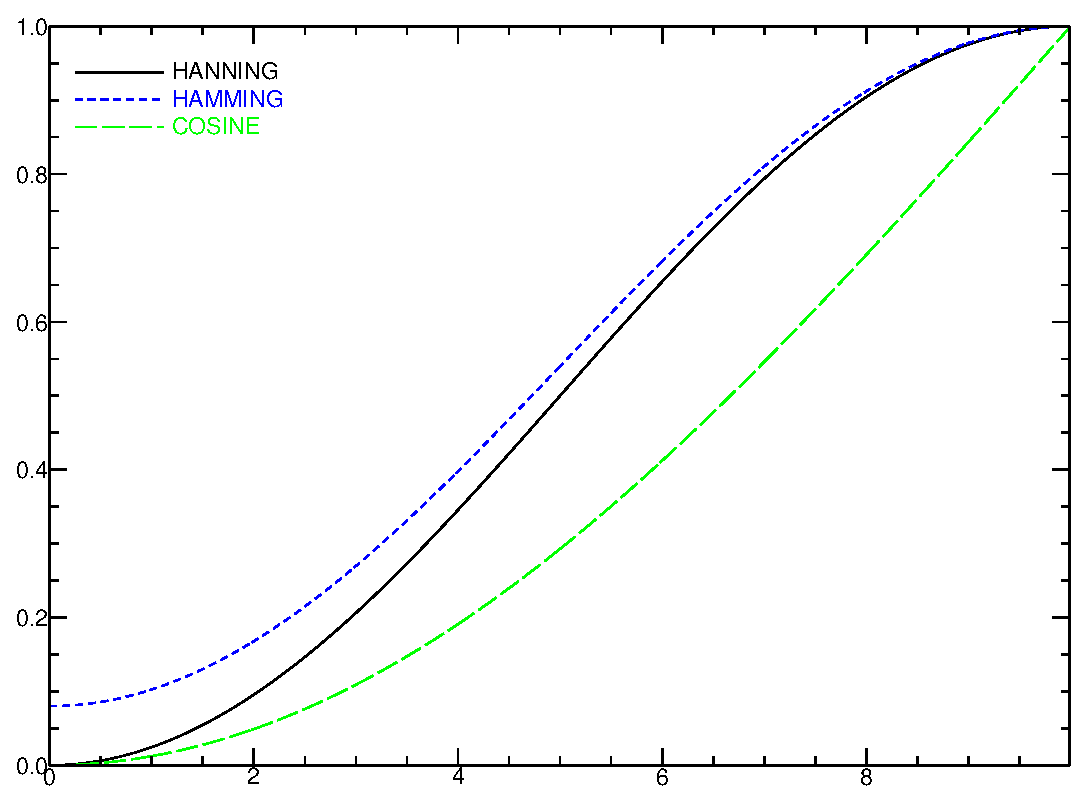
\includegraphics[width=0.8\textwidth]{taper}
\caption{taper衰减函数曲线}
\label{fig:taper-functions}
\end{figure}

\SACTitle{错误消息}
\begin{itemize}
\item[-]1301: 未读入数据文件
\item[-]1306: 对不等间隔文件的非法操作
\end{itemize}

\SACTitle{头段变量}
depmin、depmax、depmen

\SACCMD{ticks}
\label{cmd:ticks}

\SACTitle{概要}
控制绘图上刻度轴的位置

\SACTitle{语法}
\begin{SACSTX}
TICKS [ON|OFF|ONLY] [A!LL!] [T!OP!] [B!OTTOM!] [R!IGHT!] [L!EFT!]
\end{SACSTX}

\SACTitle{输入}
\begin{description}
\item [ON] 在指定的边上显示刻度,其他不变 
\item [OFF] 在指定的边上不显示刻度,其他不变 
\item [ONLY] 仅在指定的边上显示刻度,其他关闭 
\item [ALL] 所有四条边
\item [TOP] 视口上部的X轴
\item [BOTTOM] 视口的下部的X轴 
\item [RIGHT] 视口右边的Y轴 
\item [LEFT] 视口左边的Y轴 
\end{description}

\SACTitle{缺省值}
\begin{SACDFT}
ticks on all
\end{SACDFT}

\SACTitle{说明}
刻度轴可以画图形四边的一边或几边上,刻度间隔由XDIV命令控制。

\SACTitle{示例}
显示上部刻度轴,其他不变:
\begin{SACCode}
SAC> ticks on top
\end{SACCode}

关闭所有刻度轴:
\begin{SACCode}
SAC> ticks off all
\end{SACCode}

显示底部刻度轴,其余关闭:
\begin{SACCode}
SAC> ticks only bottom
\end{SACCode}

\SACTitle{相关命令}
\nameref{cmd:xdiv}、\nameref{cmd:axes}

\section{title}
\label{cmd:title}

\SACTitle{概要}
定义绘图的标题和属性

\SACTitle{语法}
TITLE [ ON | OFF | text ] [ LOCATION Top | Bottom | Right | Left ] [ SIZE Tiny | Small | Medium | Large ]

\SACTitle{输入}
\begin{itemize}
\item ON : 打开标题选项,不改变标题内容
\item OFF : 关闭标题选项 
\item text : 打开标题选项,改变标题内容,如果文本中包含空格,则标题需要用单引号括起来 
\item LOCATION location : 改变标题的位置TOP|BOTTOM|RIGHT|LEFT 
\item SIZE size : 改变标题文本尺寸TINY|SMALL|MEDIUM|LARGE 
\end{itemize}

\SACTitle{缺省值}
TITLE OFF LOCATION TOP SIZE SMALL

\SACTitle{说明}
如果这个选项打开,则在每个图形上都给出标题,标题的尺寸和位置及内容均可改变,文本质量和字体可以通过GTEXT命令设置。

\SACTitle{相关命令}
GTEXT

\SACTitle{最近修订}
January 8, 1983 (Version 8.0)

\SACCMD{trace}
\label{cmd:trace}

\SACTitle{概要}
追踪黑板变量和头段变量

\SACTitle{语法}
\begin{SACSTX}
TRACE [ON|OFF] name [name ...]
\end{SACSTX}

\SACTitle{输入}
\begin{description}
\item [ON] 打开变量追踪选项
\item [OFF] 关闭变量追踪选项
\item [name] 要追踪的黑板变量或/和头段变量名。对于头段变量,其格式为\lstinline{filename,hdrname},
    其中filename是要追踪的SAC文件名或文件号,hdrname是SAC头段变量名。
\end{description}

\SACTitle{缺省值}
\begin{SACDFT}
trace on
\end{SACDFT}

\SACTitle{说明}
该命令用于在SAC执行过程中追踪SAC黑板变量或/和头段变量的值,主要用于调试大型或复杂的宏文件。
当变量追踪选项被打开时,将显示变量的当前值。若变量追踪选项处于打开状态,则每次执行命令时将
对变量值进行检查,若变量的值发生改变则将其新值打印到终端。当变量追踪选项被关闭时,也会显示
变量的当前值。

\SACTitle{示例}
追踪黑板变量TEMP1和文件MYFILE的头段变量T0:
\begin{SACCode}
SAC> trace on temp1 myfile,t0
  TRACE  (on) TEMP1 = 1.45623
  TRACE  (on) MYFILE,T0 = UNDEFINED
\end{SACCode}

在执行命令时,SAC会检查变量值是否发生改变。若发生改变则将相关信息显示出来。假设在完成一些计算之后
改变了TEMP1,并定义了T0的值,则SAC将显示如下信息:
\begin{SACCode}
  TRACE (mod) TEMP1 = 2.34293
  TRACE (mod) MYFILE,T0 = 10.3451
\end{SACCode}

稍后的处理中TEMP1可能再次改变:
\begin{SACCode}
  TRACE (mod) TEMP1 = 1.93242
\end{SACCode}

当跟踪选项被关闭时,SAC最后一次显示变量当前值:
\begin{SACCode}
SAC> trace off temp1 myfile,t0
  TRACE (off) TEMP1 = 1.93242
  TRACE (off) MYFILE,T0 = 10.3451
\end{SACCode}

\SACCMD{transcript}
\label{cmd:transcript}

\SACTitle{概要}
控制输出到副本文件

\SACTitle{语法}
\begin{SACSTX}
TRANSCRIPT [OPEN|CREATE|CLOSE|CHANGE|WRITE|HISTORY] [FILE filename]  
    [CONTENTS ALL|ERRORS|WARNINGS|OUTPUT|COMMANDS|MACROS|PROCESSED] 
    [MESSAGE text]
\end{SACSTX}

\SACTitle{输入}
\begin{description}
\item [OPEN] 打开副本文件,并在已存在的文件底部添加副本 
\item [CREATE] 创建一个新的副本文件 
\item [CLOSE] 关闭一个已经打开的副本文件 
\item [CHANGE] 改变一个已经打开的副本文件的内容 
\item [WRITE] 写信息到一个副本文件,不改变其状态或内容 
\item [HISTORY FILE filename] 将命令行历史保存到文件 
\item [FILE filename] 定义副本文件的名字 
\item [MESSAGE text] 向副本文件中写入文本。这个信息可以用于指定正在进行的进程或指定正在
    处理的不同事件,在两次执行这个命令的过程中这个信息不保存。 
\item [CONTENTS ALL] 定义副本文件的内容为全部输入输出的信息。 
\item [CONTENTS list] 定义副本文件的内容,即包含在文件中的输入输出的类型表
\end{description}
其中list可以取:
\begin{itemize}
\item ERRORS : 执行命令期间产生的错误消息
\item WARNINGS : 执行命令期间产生的警告消息
\item OUTPUT : 执行命令期间的输出消息 
\item COMMANDS : 终端输出的原始命令 
\item MACROS : 宏文件中出现的原始命令 
\item PROCESSED : 经终端或宏处理之后的命令
\end{itemize}

\SACTitle{缺省值}
\begin{SACDFT}
transcript open file transcript contents all
\end{SACDFT}

\SACTitle{说明}
副本文件用于记录SAC执行的结果。其可以是一个完整或部分副本,可以包含一次或多次执行
的结果。你可以同时拥有5个活动的副本文件,每个文件用于追踪不同的方面。
其中的一个用途是记录终端输入的命令然后用于一个宏文件中,如下例所示。

\SACTitle{例子}
为了创建一个新的副本文件,文件名为MYTRAN,包含了除已处理命令之外的其他全部类型:
\begin{SACCode}
SAC> transcript create file mytran cont err warn out com macros
\end{SACCode}

如果之后不想把宏命令送入这个文件,你可以使用CHANGE选项:
\begin{SACCode}
SAC> transcript change file mytran contents errors warnings output commands
\end{SACCode}

为了定义一个名为MYRECORD的副本文件,其记录了终端输入的命令:
\begin{SACCode}
SAC> transcript create file myrecord contents commands
\end{SACCode}

以后,经过适当的编辑,这个文件可以用作宏命令文件,去自动执行相同的一组命令。在最后的例子中假设你需要彻夜处理许多事件。你可以设置每个事件一个副本文件(用不同的副本文件名)去记录处理的结果。另外你可以将处理所有事件得到的任何错误消息保存到一个副本文件中:
\begin{SACCode}
SAC> transcript open file errortran contents errors
SAC> transcript write message 'processing event 1'
\end{SACCode}

这些命令将放在处理每个事件的宏文件中,它假设事件名作为第一个参数带入宏。使用打开选项,
运行信息和出错信息将添加到文件的后面,第二天检查一下这个出错信息副本文件,就可以快速
查阅在处理期间是否出现了错误。

为了将保存一个命令行副本,以记录SAC当前和将来要运行的命令:
\begin{SACCode}
SCA> transcript history file .sachist
\end{SACCode}
这就在当前目录创建并写入了一个副本文件``./.sachist''。任何储存在那里的文件将被载入命令历史中。
如果这个命令位于你的启动初始化宏文件中,则每次你运行SAC时将在当前目录产生一个单独的命令行历史。
在一个新执行的SAC中,上下键将浏览完整的命令历史,你可以修改以前输入的命令并再次执行它,
如果你没有在SAC内或初始化宏文件中输入这个命令,则命令行历史将自动保存到~\lstinline{~/.sac_history}

\SACCMD{transfer}
\label{cmd:transfer}

\SACTitle{概要}
反卷积以去除仪器响应并卷积以加入其它仪器响应。

\SACTitle{语法}
\begin{SACSTX}
TRANS!FER! [FROM type [options]] [TO type [options]] 
    [FREQ!LIMITS! f1 f2 f3 f4] [PREWH!ITENING! ON|OFF|n]
\end{SACSTX}

\SACTitle{输入}
\begin{itemize}
\item FROM type : 通过谱域除法做反卷积要去除的仪器类型。 
\item TO type : 通过谱域乘法做卷积来加入的仪器类型。 
\item FREQLIMITS f1 f2 f3 f4:设定频率段,以处理超高频和超低频信号。
\item PREWHITENING ON|OFF|n:预白化处理。
\end{itemize}

\SACTitle{缺省值}
\begin{SACDFT}
trans from none to none
\end{SACDFT}

\SACTitle{说明}
关于仪器响应以及transfer命令,参考~``\nameref{sec:instrument-response}''一节。

在TRANSFTER中默认仪器的输入输出都是位移,在SAC中定义为NONE。
因而如果FROM类型或者TO类型未指定,SAC会假定其为NONE。

若输出仪器是NONE,则SAC头段中的IDEP将设置为DISPLACEMENT(单位为nm). 如果TRANSFER选择为TO VEL
或TO ACC,SAC中的头段变量IDEP将根据内存中的波形而改变。

如果TO指定为除NONE、VEL、ACC外的其他类型,内存中的波形将被卷积上相应的仪器类型。如果FROM仪器类型是NONE,则不会去除仪器响应,原始的地震道数据认定为位移,这常用于向合成地震图中加入仪器响应。

在同一个SAC会话中,当第二次调用TRANSFER时一定要特别小心,因为第二次调用TRANSFER时会使用第一次调用时的参数,除非显式指定其参数。

所有的地震仪在0频率处都具有零响应。当做反卷积但不卷积其他响应的时候(e.g. ``TO NONE''),就有必要修改超低频率处的响应以防止频率域除0。在高频区域,信噪比通常很低,因而有必要对其响应进行抑制。FREQLIMITS即可满足此要求。FREQLIMITS包含了低通和高通的尖灭器(taper)。四个频率满足f1<f2<f3<f4,尖灭器在f2和f3间为1,在f1以下和f4以上为0。频率f1和f2确定了高通滤波器的特性,频率f3和f4指定了低通滤波器的特性。f1与f2之间以及f3与f4之间分别为余弦波的四分之一个周期。

如果你想要一个低通滤波器但在低频处不滤波,一种方法是设置f1=-2和f2=-1;如果你想要一个高通滤波器但在高频处不滤波,对于Nyquist频率为0.5,设置f3=10和f4=20。

注意:由于滤波器还有零相位,因而其是非因果。如果数据点数npts不为2的指数幂次,会导致在频段(f1,f4)之外振幅不为0。如果想要数据点数为2的幂次方个,可以参考SAC中的CUT命令。

缺省值中是没有FREQLIMITS选项的,在使用FREQLIMITSEVALRESP和POLEZERO选项时,应该加上FREQLIMITS选项以处理超高频和超低频。

PREWHITENING控制数据的预白化:
\begin{itemize}
\item PREWHITENING: 预白化可以将输入时间序列在变换到频率域之前,进行谱的平化。这	会减小谱值的动态范围,并提高数据在高频的计算精度。默认prewhitening是关闭的。参见WHITEN命令。
\item PREWHITENING ON : 在谱操作之前在频率域进行谱白化,并在谱操作后在时间域做谱白化的补偿。
\item PREWHITENING OFF : 关闭预白化。
\item PREWHITENING n : 打开预白化选项并设置其阶数。如果打开预白化但不指定阶数,则缺省n=6,除非在WHITEN命令中已经修改了预白化阶数。
\end{itemize}

\SACTitle{例子}
为了将NYKM.Z去除台站RSTN的仪器响应,并应用DSS的仪器响应:
\begin{SACCode}
SAC> read nykm.z
SAC> trans from rstn subtype nykm.z to dss prew off
\end{SACCode}  	

为了去除LLL宽频带仪器响应,应用SRO仪器响应,并对频带做尖灭及预白化:
\begin{SACCode}
SAC> read abc.z
SAC> trans from lll to sro freq .02 .05 1. 2. prew 2
\end{SACCode}
得到的地震数据的通带,在0.05Hz到1Hz是平的,在0.02Hz以下及2Hz以上为0。

在反卷积前在时间域做二阶预白化,在卷积之后该效应被移除。

为了将电磁仪器响应转换为位移:
\begin{SACCode}
SAC>  read xyz.z
SAC>  transfer from elmag freep 15. mag 750. to none
\end{SACCode}

\SACCMD{traveltime}
\label{cmd:traveltime}

\SACTitle{概要}
根据预定义的速度模型计算指定震相的走时。

\SACTitle{语法}
\begin{SACSTX}
T!RAVEL!TIME [MODEL string] [PICKS number] [PHASE phase list] 
    [VERBOSE|QUIET] [M|KM]
\end{SACSTX}

\SACTitle{输入}
\begin{itemize}
\item MODEL : iasp91或ak135,缺省为iasp91
\item Picks : 如果number值位于0到9,则第一个震相的到时将储存在头段Tn中。如果命令行选项中没有包含PICKS,VERBOSE就会打开并显示震相到时而不写入头段。
\item PHASE : 要pick或显示的震相列表,如果有PICKS n选项,则则震相到时以及其标签将写入到头段Tn和KTn中。 
\item VERBOSE|QUIET : 若使用VERBOSE,则震相走时将以相对发震时刻(O)和文件起始时间(B)两种方式显示;若使用QUIET,则不在屏幕上显示到时,若二者都没有显示,则显示TRAVELTIME命令使用的深度 
\item M|KM : EVDP的单位为m或者km。
\end{itemize}

\SACTitle{缺省值}
\begin{SACDFT}
MODEL iasp91 KM PHASE P S Pn Pg Sn Sg
\end{SACDFT}

\SACTitle{说明}
该命令使用\href{http://www.iris.edu/software/downloads/processing/}{iaspei-tau}
程序计算走时,要求内存中的波形文件的事件和台站位置以及发震时刻必须定义。

内存中所有文件拾取的震相的到时存储在头段变量Tn中,其中n的范围为0到9。计算的走时是相对于发震时刻(O)的,但存储在Tn中的时间是相对于文件起始时间(B)。

走时表根据地震深度及震中距获得走时,震中距(GCARC)使用球三角几何,根据事件和台站经纬度计算。

由于历史原因,事件深度EVDP以前的单位为m,RDSEED产生的SAC波形数据单位为m。

在v101.5中,默认的EVDP单位为km,但由于很多波形数据EVDP仍然为m,这里引入这个命令选项以指定深度单位。

在SAC2000中,命令TRAVELTIME位于子程序SSS中,当前版本(V101.5)没有SAC2000版本的全部功能,但可以不用进入SSS而直接运行。

\SACTitle{例子}
区域事件,使用默认震相:
\begin{SACCode}
SAC> fg seismo
SAC> traveltime 
traveltime: depth: 15.000000
traveltime: error finding phase P       
traveltime: error finding phase S       
traveltime: setting phase Pn       at 10.464321 s [ t = 51.894321 s ]
traveltime: setting phase Pg       at 22.904724 s [ t = 64.334724 s ]
traveltime: setting phase Sn       at 50.047722 s [ t = 91.477722 s ]
traveltime: setting phase Sg      at 66.414337 s [ t = 107.844337 s ]
\end{SACCode} 

对于区域事件,初至波为Pn或Pg,因而这里没有P波到达,对上面的例子,拾取不会写入头段中。
\begin{SACCode}
SAC> fg seismo
SAC>  traveltime picks 0 phase Pn Pg Sn Sg
traveltime: depth: 15.000000
SAC> lh AMARKER T0MARKER T1MARKER T2MARKER T3MARKER
AMARKER = 10.464                     
T0MARKER = 10.464           (Pn)
T1MARKER = 22.905           (Pg)
T2MARKER = 50.048           (Sn)
T3MARKER = 66.414           (Sg)
SAC> write seismo-picks.z
\end{SACCode}
可以看到已经将A定义为Pn的到时,文件seismo-picks.z将有T0到T3四个头段,命令PLOT1可以看到有各震相在相应到时处有标签名。
注意尽管VERBOSE没有开启,深度(单位km)还是会被打印出来。这是为了保证用户对EVDP的单位有正确的了解,可以通过QUIET选项取消深度的显示。

下面例子给出的波形文件是由RDSEED(V5.0)产生的,EVDP单位为m:
\begin{SACCode}
SAC> r 2008.052.14.16.03.0000.XC.OR075.00.LHZ.M.SAC
SAC> lh evdp
evdp = 6.700000e+03
SAC> traveltime M picks 0
traveltime: depth: 6.700000 km
SAC> lh t0marker t1marker t2marker t3marker
t0marker = 61.48            (Pn)        
t1marker = 76.413           (Pg)
t2marker = 109.66           (Sn)  
t3marker = 132.11           (Sg)
SAC> ch evdp (0.001 * :1,evdp:)
SAC> setbb station :1,KSTNM:
SAC> write %station%.z
\end{SACCode}
保存的文件OR075.z单位为km,并且各个震相Pn、Pg、Sn及Sg都有注释。震相名是大小敏感的,具体参见iaspei-tau的文档。

\section{tsize}
\label{cmd:tsize}

\SACTitle{概要}
控制文本尺寸属性

\SACTitle{语法}
TSIZE [ Tiny | Small | Medium | Large v ] [ RATIO v ] [ OLD | NEW ]

\SACTitle{输入}
\begin{itemize}
\item size v : 改变文本尺寸之一的值为v 
\item RATIO v : 改变文本的宽高比为v 
\item OLD : 将所有文本尺寸值设置为其旧值,这些旧值用在SAC 9之前的版本中 
\item NEW : 改变所有文本尺寸值为SAC初始化时的缺省值。
\end{itemize}

\SACTitle{缺省值}
TSIZE RATIO 1.0 NEW

\SACTitle{说明}
大多数的文本注释命令(TITLE, XLABEL, FILEID等)允许你改变要显示的文本的尺寸。你可以从四个已命名的尺寸中选择(TINY, SMALL, MEDIUM, 和LARGE.)。每一个命名尺寸有一个初始值,如下表所示。其尺寸是一个字符相对整个视窗的高度。有些时候你想要使用一些不同与默认尺寸的注释。TSIZE允许你重新定义这四个已命令的尺寸。你也可以使用这个命令改变字符的宽-高比。
\begin{center}
\begin{tabular}{lccccc}
\toprule
NAME	&	A	&	B	&	C	&	D	&	E	\\
\midrule
TINY 	& 0.015 &   66 	&  50  	&	68  &	110	\\
SMALL	& 0.020 &	50  &  37  	&	66  &	82	\\
MEDIUM  & 0.030 &	33  &  25  	&	44  &	55	\\
LARGE	& 0.040 &	25  &  18  	&	33  &	41	\\
\bottomrule
\end{tabular}
\end{center}

上面做各列的定义如下:
\begin{itemize}
\item A 自如相对整个视窗的高度
\item B 全视窗下文本的行数
\item C 正常视窗下文本的行数。正常视窗是指x为0.到1.,y为0.到0.75
\item D 正常视窗中,每行的最小字符数
\item E 正常视窗中每行字符的平均数
\end{itemize}

\SACTitle{例子}
为了改变MEDIUM的定义,并使用它创建一个特别尺寸的标题:
\begin{SACCode}
SAC> TSIZE MEDIUM 0.35
SAC> TITLE 'Rayleigh Wave Spectra' SIZE MEDIUM
SAC> PLOT2
\end{SACCode}

为了重置尺寸定义到其缺省值:
\begin{SACCode}
SAC> TSIZE NEW
\end{SACCode}

\SACTitle{相关命令}
TITLE, XLABEL, FILEID, PLOTC

\SACTitle{最近修订}
July 22, 1991 (Version 9.1)


\SACCMD{unsetbb}
\label{cmd:unsetbb}

\SACTitle{概要}
删除黑板变量

\SACTitle{语法}
\begin{SACSTX}
UNSETBB ALL|variable ...
\end{SACSTX}

\SACTitle{输入}
\begin{description}
\item [ALL] 删除当前定义的全部黑板变量 
\item [variable] 删除黑板变量variable 
\end{description}

\SACTitle{说明}
参见\nameref{cmd:setbb}命令的说明

\SACTitle{例子}
一次删除多个黑板变量:
\begin{SACCode}
SAC> unsetbb c1 c2 x
\end{SACCode}

删除所有黑板变量:
\begin{SACCode}
SAC> unsetbb all
\end{SACCode}

\SACTitle{相关命令}
\nameref{cmd:setbb}、\nameref{cmd:evaluate}、\nameref{cmd:getbb}

\section{unwrap}
\label{cmd:unwrap}

\SACTitle{概要}
计算振幅谱并展开相位谱

\SACTitle{语法}
UNWRAP [ FILL ON | OFF | n ] [ INTTHR v ] [ PVTHR v ]

\SACTitle{输入}
\begin{itemize}
\item FILL ON | OFF : 打开/关闭零点填充选项 
\item FILL n : 打开零点填充选项并将填充值设置为n 
\item INTTHR v : 改变积分阀值常量为v 
\item PVTHR v : 改变主阀值常量为v 
\end{itemize}

\SACTitle{缺省值}
UNWRAP FILL OFF INTTHR 1.5 PVTHR 0.5

\SACTitle{说明}
这个命令将内存中的时间序列数据转换为谱数据,其包含了振幅谱和展开相位谱的频谱数据。这个过程作用于具有光滑变换相位的数据。数据在转换之前补0以使数目为2的幂数倍,你可以使用FILL选项指定大量补充零点。

这是Tribolet算法的工具程序。其中用两种方法来估算在任何频率的展开相位。一个是通过快速傅氏变换做相位导数的数字积分。如果需要得到一个稳定一致的估算常数,则可将这个梯形积分的步长在每个频率上对分。你可以使用INTTHR选项控制这个验算的阀值,此值单位为弧度。减少INTTHR将改进相位计算结果,然而这个值太小时,会导致发散。

算法中使用的第二个方法是使用反正切函数先计算相位的主值。展开相位的计算方法是相位主值加上2*PI的整数倍,直到相位的突变小于给定的阀值为止。可以使用PVTHR选项控制这个验算的阀值。与上一个算法类似,减少这个阀值将改进相位估算的结果,但也增加了无解的可能性。

这两个阀值的初值通常经验地取为:
\[ \pi/4 < PVTHR < INTTHR < 2\pi \]

\SACTitle{错误消息}
\begin{itemize}
\item[-]1301: 未读入数据文件
\item[-]1306: 对不等间隔文件非法操作
\item[-]1606: 超过DFT允许的最大数据点数
\end{itemize}

\SACTitle{警告消息}
\begin{itemize}
\item[-]1610: 对文件中数据点的相位展开失败。
	\begin{itemize}
	\item[-]调整阀值然后重试
	\end{itemize}
\end{itemize}

\SACTitle{头段变量改变}
B, E 和 DELTA 分别改变为变换的起始频率、结束频率和采样频率。原始的B,E和DELTA被保存在为SB、SE、SDELTA,当进行反变换时将值带回。

\SACTitle{限制}
目前可以转换的数据最大长度为4096。

\SACTitle{参考文献}
Tribolet, Jose M.; "A New Phase Unwrapping Algorithm"; IEEE Transactions on Acoustics, 	Speech, and Signal Processing; Vol. ASSP-25, No 2, April 1977;page 170.

\SACTitle{最近修订}
January 8, 1983 (Version 8.0)


\SACCMD{vspace}
\label{cmd:vspace}

\SACTitle{概要}
改变图形的最大尺寸和形状

\SACTitle{语法}
\begin{SACSTX}
VSP!ACE! FULL|v
\end{SACSTX}

\SACTitle{输入}
\begin{itemize}
\item FULL : 使用整个视窗,这是可能的最大屏幕或窗口尺寸 
\item v : 使视窗比y:x为v,具有这个纵横比的最大的区域称为视窗 
\end{itemize}

\SACTitle{缺省值}
\begin{SACDFT}
VSPACE FULL
\end{SACDFT}

\SACTitle{说明}
视窗代表了屏幕上可以用于绘图的部分。视窗形状和尺寸在不同图形设备之间有很大的变化。
\begin{enumerate}
\item 尽管在尺寸上有很大不同,许多图形终端都具有0.75的纵横比。
\item SGF文件的纵横比为0.75,其大约是标准的8.5*11英寸纸张的纵横比。
\item  由XWINDOWS或SUNWINDOWS图形设备建立的窗口可以有你想要的任意纵横比
\end{enumerate}

这个命令可以控制纵横比,从而使你能够控制图形的形状缺省绘图是在整个视窗上,如果确定了一个纵横比,则视窗就是设备上具有这个纵横比的最大区域。

当你使用PLOTC命令在交互设备上建立一张图,并且最终要将它发送到SGF设备上,这个命令特别有用,在绘制任何图形之前,必须设置纵横比为0.75。这将保证图形在SGF文件上与在交互设备上相同。如果你要建立一个独立于图形设备的正方形视窗,则可以简单地设置纵横比为1.0

\SACCMD{wait}
\label{cmd:wait}

\SACTitle{概要}
控制SAC在绘制多个图形时是否暂停

\SACTitle{语法}
\begin{SACSTX}
WAIT [ON|OFF|EVERY]
\end{SACSTX}

\SACTitle{输入}
\begin{description}
\item [ON] 按常规模式打开等待选项 
\item [OFF] 关闭等待选项 
\item [EVERY] 每个图形之间均等待
\end{description}

\SACTitle{缺省值}
\begin{SACDFT}
wait on
\end{SACDFT}

\SACTitle{说明}
当你读取了多个数据文件并使用PLOT绘制,每个文件将产生一个框架,如果你绘制到终端,
正常情况下SAC将在每张图后暂停并发送信息``WAITING''到终端。然后你可以键入回车看到下一张图,
或输入``GO''使SAC不暂停地绘制剩下的图形,或键入``KILL''终止绘制这组文件。SAC绘制最后
一张图之后不再暂停,因为通常的输入提示符提供了相同的功能。当这个选项关闭时,SAC在不
同的绘图之间不暂停。在每个图形模式下,SAC不仅在用PLOT命令产生的绘图之间,而且在绘制
每个图形时都暂停。如果你是在命令文件或者作业控制程序的控制下使用SAC,那么这一点将很有用。

\SACCMD{whiten}
\label{cmd:whiten}

\SACTitle{概要}
平滑输入的时间序列的频谱。

\SACTitle{语法}
\begin{SACSTX}
W!H!IT!EN! n [F!ILTER!D!ESIGN!]
\end{SACSTX}

\SACTitle{输入}
\begin{itemize}
\item n :  阶数(极数)。这个数越大,结果数据就越平滑。高阶可以更好的清除一些数据,但是也可能会导致对数据处理过多而丢掉一些重要的数据。默认值为6。 
\item FD : 进行一些类似于filterdesign的命令,使用白化系数,设计一个白化滤波器。详情可以参考filterdesign命令。
\end{itemize}

\SACTitle{缺省值}
\begin{SACDFT}
whiten 6
\end{SACDFT}


\SACTitle{说明}
对数据中加入白噪声。平滑输入时间序列的频谱。当这个命令在谱分析命令(比如子程序SPE中的命令、transfer或spectrogram)之前执行,其减少了频谱值的动态范围,提供了对地震数据高频操作的精度。

WHITEN可以在SPE子程序内部调用,或者从SAC的主shell中调用。SPE中的WHITEN和主shell中的WWHITEN分别有不同的阶数。在主shell中,你可以调用WHITEN 4,下一次在主shell中调用WHITEN时阶数为4,但是在SPE中调用WHITEN时依然是缺省的6阶,除非你在SPE的命令行中进行了修改。进一步,SPE中的阶数与SPE COR命令的PREWHITEN选项是一样的(设置了一个其他的也就设置了)。当然主shell中WHITEN命令与TRANSFER命令中的PREWHITEN选项也是一样的。

\SACTitle{相关命令}
\nameref{cmd:transfer}

\section{whpf}
\label{cmd:whpf}

\SACTitle{概要}
将辅助内容写入HYPO格式的震相拾取文件中

\SACTitle{语法}
WHPF IC n m

\SACTitle{输入}
\begin{itemize}
\item IC n m  在第18和19列插入带有两个整数的n和m的指令卡。n的允许值为0、1、5,m的允许值为0、1、9。
\end{itemize}

\SACTitle{说明}
``指令卡''用于分开在HYPO文件中的不同事件,参见HYPO71手册。关闭一个已经打开的HYPO震相拾取文件(CHPF)或者退出SAC时,将自动添加``10''指令卡到震相读取文件中。

\SACTitle{错误消息}
\begin{itemize}
\item[-]1908: HYPO震相拾取文件未打开
\end{itemize}

\SACTitle{相关命令}
CHPF, OHPF

\SACTitle{参考文献}
W.H.K. Lee and J.C. Lahr; HYPO71 (Revised): A Computer Program for Determining 	Hypocenter, Magnitude, and First Motion Pattern of Local Earthquakes; U. S. Geological 	Survey report 75-311.

\SACTitle{最近修订}
March 20,1992 (Version 10.6e)

\SACCMD{width}
\label{cmd:width}

\SACTitle{概要}
控制所选图形设备的线宽

\SACTitle{语法}
WIDTH  [ ON | OFF | linewidth ] [ SKELETON width ] [ INCREMENT ON | OFF ] [ LIST STANDARD | widthlist ]

其中linewidth, width, widthlist是整数值

**注意** LIST选项必须放在命令的最后

\SACTitle{输入}
\begin{itemize}
\item WIDTH ON : 打开WIDTH选项但是不改变当前线宽值 
\item WIDTH OFF : 关闭width选项 
\item WIDTH linewidth : 改变数据的线宽为linewidth并打开WIDTH选项。 
\item SKELETON width : 改变图形边框宽度为width并打开WIDTH选项 
\item INCREMENT {ON} : 按照widthlist表中的次序,依次改变一个宽度值 
\item INCREMENT OFF : 关闭线宽递变功能 
\item LIST widthlist : 改变宽度列表的内容。输入宽度列表。设置数据宽度为列表中的第一个宽度,并打开width选项。 
\item LIST STANDARD : 设置为标准线宽列表,设置数据宽度为列表中的第一个宽度,并打开width选项。 
\end{itemize}

\SACTitle{缺省值}
WIDTH OFF SKELETON 1 INCREMENT OFF LIST STANDARD

\SACTitle{说明}
这个命令控制那些可显示很多不同线宽的设备的宽度属性。数据宽度是指绘制数据文件时使用的宽度。数据宽度可在每个数据文件绘图之后,按照宽度表中的次序自动地变成另一个宽度。边框宽度是用于绘制坐标轴的宽度。在SKELETON选项下,仅修改坐标轴的宽度。网格、文本、标签和框架号,总是用1号细线显示。
如果在同一张绘图中同时绘制几个数据文件,你也许需要每个文件有不同的宽度。此时可使用INCREMENT选项。在这个选项打开时,每次绘制一个数据文件后,都按照宽度表中的次序自动地变成另一个宽度。宽度值和次序在标准宽度表中为:
\begin{SACCode}
1, 2, 3, 4, 5, 6, 7, 8, 9, 10
\end{SACCode}
你可以使用LIST选项改变这个表的次序或内容。这个命令常用于重叠绘图(参见PLOT2),此时你可能需要每张图上的数据宽度都按相同的顺序排列。

\SACTitle{例子}
选择自动变换的数据宽度起始值为1:
\begin{SACCode}
SAC> WIDTH 1 INCREMENT
\end{SACCode}

边框宽度起始值为2,并按1、3、5的增量变化:
\begin{SACCode}
SAC> WIDTH SKELETON 2 INCREMENT list 1 3 5
\end{SACCode}

\SACTitle{最近修订}
June 20, 1992 (Version 10.6e)


\SACCMD{wiener}
\label{cmd:wiener}

\SACTitle{概要}
设计并应用一个自适应Wiener滤波器

\SACTitle{语法}
\begin{SACSTX}
W!IE!N!E!R [WINDOW pdw] [NCOEFF n] [MU OFF|ON|v] [EPS ILON OFF|ON|e]
\end{SACSTX}

\SACTitle{输入}
\begin{itemize}
\item WINDOW pdw : 设置滤波器设计窗口为pdw。关于pdw参见CUT命令 
\item NCOEFF n : 设置滤波器系数为n个 
\item MU off | on | v : 设置自适应步长参数 
\item Off : 将mu设置为0 
\item On : 将mu设置为mu = 1.95 / Rho(0)。其中Rho(0)是pdw中延迟为0时的自相关系数。 
\item v : 设置 mu = v. 
\item EPSILON e :  Set ridge regression parameter to epsilon. 
\end{itemize}

\SACTitle{缺省值}
\begin{SACDFT}
wiener window b 0 10 ncoeff 30 mu off epsilon off
\end{SACDFT}

\SACTitle{说明}
误差预测滤波器使用Yule-Walker方法,从指定的部分数据窗中由自相关函数给出。这个窗口可以是文件的任何部分,然后滤波器应用到这个个信号,即信号由残差序列置换。这个滤波器可以用作预白化或用作瞬时信号的检波预处理器。对MU指定非0值,滤波器可作成时域自适应的,大MU可能会导致不稳定。

\SACTitle{例子}
下面的命令将应用一个非自适应滤波器,将第一个十秒指定为窗:
\begin{SACCode}
SAC> wiener window b 0 10 mu 0.
\end{SACCode}

下面命令将应用带40个系数的滤波器,指定设计窗为从文件开始到第一个到时前1秒:
\begin{SACCode}
SAC> wiener ncoeff 40 window b a -1
\end{SACCode}

\SACTitle{头段变量改变}
depmin, depmax, depmen

\SACTitle{错误消息}
\begin{itemize}
\item[-]1301: 未读入数据文件
\item[-]1306: 对不等间隔文件的非法操作
\item[-]1307: 对谱文件的非法操作
\item[-]1608: 不良的Wiener滤波器噪声窗口(滤波器设计窗口不在文件窗口内,或用于窗口的
    头段变量值未定义)
\end{itemize}

\SACTitle{警告消息}
\begin{itemize}
\item[-]1609: Wiener滤波器数字不稳定
\end{itemize}

\SACTitle{相关命令}
\nameref{cmd:cut}

\SACCMD{wild}
\label{cmd:wild}

\SACTitle{概要}
设置读命令中用于扩展文件表的通配符

\SACTitle{语法}
WILD [ ECHO ON | OFF ] [ SINGLE char ] [ MULTIPLE char ] [ CONCATENATION chars ]

\SACTitle{输入}
\begin{itemize}
\item ECHO ON : 打开扩展文件表回应开关,当这个选项打开并且在文件表中有通配符时才有回应。 
\item ECHO OFF : 关闭扩展文件表回应开关 
\item SINGLE char : 改变用于匹配单个字符的通配符 
\item MULTIPLE char : 改变用于匹配多个字符的通配符 
\item CONCATENATION chars : 改变用于字符串两侧的两个字符连接串 
\end{itemize}

\SACTitle{缺省值}
\begin{center}
\begin{tabular}{llll}
\toprule
选项	&	UNIX	&	VAX		&	PRIME	\\
\midrule
ECHO	&	ON 		&	ON 		&	ON		\\
SINGLE  &	?  		&	?  		&	+		\\
MULTIPLE&	* 		&	* 		&	'		\\
CONCATENATION& [,] & 	(,)  	&	[,]		\\
\bottomrule
\end{tabular}
\end{center}

\SACTitle{说明}
很多现代操作系统都提供了通配符特性,也可以称为文件扩展。它是一个可以让你使用简短文件名以及简单的简写形式去指定一组文件的代号。SAC在READ、READTABLE以及READHDR命令中使用通配符及一些扩展名,使用这些代号,你可以很容易地访问一些文件组:
\begin{itemize}
\item 所有以字母``abc''开头的文件
\item 所有以``z''结尾的文件
\item 所有文件名中严格包含三个字母的文件
\end{itemize}

通配符代号有三个元素。对于不同的系统三个元素会有不同的缺省符。你可以使用这个命令改变通配符。多重匹配字符(``*'')用于匹配字符串中任意字符串,包括空字符串。单个匹配符(``?'')用于匹配任意单个字符。连接符号(``[''和``]'')用于包围由逗号分隔的要匹配的字符串。在这个字符串中,可以包含单通配符或多通配符。

SAC使用通配符完成文件名的扩展,通常有几个步骤:
\begin{enumerate}
\item 如果标识目录部分存在的话将将其去掉,否则使用当前目录
\item 做系统调用,以得到目录中所有文件的列表
\item 如果在标识中是一个连接表,就用其他字符形成连接表中每个字符的新的标识,然	  后匹配它们到文件表中。如果没有连接表标识,则可简单匹配标识到文件表
\item 去掉形成扩展文件表的所有重复的匹配
\item 如果需要,回显扩展文件表
\item 试着将扩展文件表读入内存
\end{enumerate}

每个操作系统都使用一些不同的步骤在一个目录中存取文件。上面第一步的系统调用反映了这些不同。例如,在UNIX中以字母顺序显示文件名,但在PRIME或VAX上就不是这样。在PRIME目录中文件次序是随意的。这些不同反映在扩展文件表的文件次序上。你可以用各种不同的通配符和连接表进行实验,以确定扩展文件表中的文件次序是否重要。

下例将帮助你理解怎样使用这些通配符元素,一个有用的特征是SAC保存包含在连接表上的字符串,当你输入一个空表,则前面的表将被重复使用,这可以节省许多输入的操作。

\SACTitle{例子}
假定当前目录中包含如下次序的文件:

ABC DEF STA01E STA01N STA01Z STA02E STA02N STA02Z STA03Z

同样假定扩展文件设置回显,下面显示怎样使用各种通配符去将上面文件表的一部分读入内存:
\begin{SACCode}
SAC> READ S*
 STA01E STA01N STA01Z STA02E STA02N STA02Z STA03Z
SAC> READ *Z
 STA01Z STA02Z STA03Z
SAC> READ ???
 ABC DEF
SAC> READ STA01[Z,N,E]
 STA01Z STA01N STA01E
SAC> READ *[Z,N,E]
 STA01Z STA02Z STA03Z STA01N STA02N STA01E STA02E
SAC> READ *1[Z,N,E] *2[ ]
 STA01Z STA01N STA01E STA02Z STA02N STA02E
\end{SACCode}

\SACTitle{限制}
在一个标识中只可以有一个连接串

\SACTitle{相关命令}
READ, READALPHA, READHDR

\SACTitle{最近修订}
May 15, 1987 (Version 10.2)

\SACCMD{window}
\label{cmd:window}

\SACTitle{概要}
设置图形窗口被创建时的位置和形状

\SACTitle{语法}
\begin{SACSTX}
WINdow n [X!SIZE! xwmin xwmax]  [Y!SIZE! ywmin ywmax]
\end{SACSTX}

\SACTitle{输入}
\begin{itemize}
\item n : 要设置属性的图形窗口号,n取值1到10. 
\item X xwmin xwmax : 设置图形窗口相对屏幕的水平位置。xwmin是窗口左边界位置,xwmax是窗口右边界位置,相对屏幕的坐标取值为0.0到1.0  
\item Y ywmin ywmax : 设置图形窗口相对屏幕的垂直位置,其他与X选项含义相同。
\end{itemize}

窗口位置缺省值(前5个): 
\begin{table}[!ht]
\centering
\caption{SAC标准窗口}
\begin{tabular}{ccccc}
\toprule
 n & xwmin & xwmax & ywmin & ywmax  \\
\midrule
 1 & 0.05  & 0.85  & 0.05  & 0.60 \\
 2 & 0.07  & 0.87  & 0.07  & 0.62 \\
 3 & 0.09  & 0.89  & 0.09  & 0.64 \\
 4 & 0.11  & 0.91  & 0.11  & 0.66 \\
 5 & 0.13  & 0.93  & 0.13  & 0.68 \\
\bottomrule
\end{tabular}
\end{table}

\SACTitle{说明}
参见beginwindow命令

\SACTitle{例子}
为了设置窗口3的垂直位置而不修改其水平位置:
\begin{SACCode}
SAC> window 3 y 0.1 0.9
\end{SACCode}

\SACCMD{write}
\label{cmd:write}

\SACTitle{概要}
将内存中的数据写入磁盘

\SACTitle{语法}
\begin{SACSTX}
W!RITE! [SAC|ALPHA|XDR] [DIR OFF|CURRENT|name] [KSTCMP] 
    [OVER|APPEND text|PREPEND text|DELETE text|CHANGE text1 text2] filelist
\end{SACSTX}

\SACTitle{输入}
\begin{itemize}
\item no arguments : 使用以前的格式和写文件列表 
\item SAC : 将SAC二进制文件格式写入磁盘 
\item ALPHA : 写SAC字符数字型数据文件 
\item SEGY : 写IRIS/PASSCAL的SEGY格式文件。这个文件允许一个文件包含一个波形而非一个分量,SEGY格式只能用于等间距时间序列文件。在SAC中SCALE字段被忽略,因为SAC将波形以一系列浮点数的形式储存起来,而SEGY则以一系列长整数储存。从SAC中得到的数据将被归一到允许的最大整数。SEGY中的scale字段用于决定将波形复原到SAC文件时需要的因子。
\item XDR : 用SAC二进制xdr格式写文件。这个格式用于实现不同构架的二进制数据的转换 
\item DIR OFF : 关闭目录选项,即写入当前目录 
\item DIR CURRENT : 打开目录选项并设置写目录为当前目录 
\item DIR name : 打开目录选项并设置写目录为name。将所有的文件写入目录name中,其可以是相对或绝对路径 
\item KSTCMP : 使用KSTNM和KCMPNM头段变量为内存中每个数据文件定义一个文件名。生成的文件名将检查是否唯一,如果不唯一,则在文件名后加序号以避免冲突
\item OVER : 使用当前读文件表作为写文件表,用内存中的文件覆盖磁盘上的文件 
\item APPEND text : 通过在当前读文件列表后附加文本创建写文件表 
\item PREPEND text : 通过在当前读文件列表前附加文本创建写文件表 
\item DELETE text :  通过在当前读文件列表中删除第一次出现的text创建写文件表 
\item CHANGE text1 text2 : 通过将当前读文件表中每个文件名第一次出现的text1修改为text2来创建写文件表 
\item filelist : 将写文件表设置为filelist,这个列表可以包含文件名、相对/绝对路径,不可以包含通配符。 
\end{itemize}

\SACTitle{缺省值}
\begin{SACDFT}
write sac
\end{SACDFT}

\SACTitle{说明}
这个命令允许你在数据处理的任一步将结果写入磁盘。这个命令运用于几种磁盘文件格式。内存中的每个文件都将不经过裁剪或减采样地写入磁盘。

多数情况下,需要使用SAC数据文件格式。这是供快速读写的压缩二进制文件格式。它包含一个较大的头段和一段或两段数据记录。详情参见具体章节。

你可以直接指定写文件名,也可以通过修改内存中的当前文件名间接地指定它们。OVER选项把写文件表设置到读文件表。它用于覆盖包含当前内存的数据的读入的最后一组磁盘文件。APPEND, PREPEND, DELETE,CHANGE选项通过以所需要的方式修改每个读文件名的方式建立一个写文件表,这在宏命令中非常有用,在宏命令中你通常需要自动处理大量数据文件,并保持输出文件风格的一致。当选择这四个选项中的一个时,便可输出写文件,这使你可以看到实际使用的文件名。

\SACTitle{例子}
对一组数据文件进行滤波,然后将结果存入一组新数据文件:
\begin{SACCode}
SAC> read d1 d2 d3
SAC> lowpass butter npoles 4
SAC> write f1 f2 f3
\end{SACCode}

也可以使用CHANGE选项完成这一操作:
\begin{SACCode}
SAC> read d1 d2 d3
SAC> lowpass butter npoles 4
SAC> write change d f
\end{SACCode}

注意这种情况下SAC输出写文件表,若用滤波数据置换原始数据,则上例的第三行要变成:
\begin{SACCode}
SAC> write over
\end{SACCode}

\SACTitle{错误消息}
\begin{itemize}
\item[-]1301: 未读入数据文件
\item[-]1311: 没有要写的文件列表
\item[-]1312: 写文件表中文件数目错误(写文件表中的文件数必须等于读入内存中的文件的数目)
\item[-]1303: 文件未打开覆盖写标志(头段变量LOVROK是.FALSE. )
\end{itemize}

\SACTitle{相关命令}
\nameref{cmd:read}

\SACCMD{writebbf}
\label{cmd:writebbf}

\SACTitle{概要}
将一个暂存块变量写入磁盘

\SACTitle{语法}
WriteBBF {file}

\SACTitle{输入}
\begin{itemize}
\item file : 暂存块变量文件的名字,其可以是简单文件名或相对/绝对路径。
\end{itemize}

\SACTitle{缺省值}
WRITEBBF BBF

\SACTitle{说明}
这个命令让你能够将暂存块变量写入磁盘,其可以稍后用READBBF命令读入SAC,这个特性允许你保存SAC某次执行得到信息到另一个。你也可以在自己的程序中写代码去访问这些暂存块变量文件的信息。这使你可以在自己的程序与SAC之间交换信息。

\SACTitle{相关命令}
READBBF, SETBB, GETBB

\SACTitle{最近修订}
May 15, 1987 (Version 10.2)


\section{writecss}
\label{cmd:writecss}
\SACTitle{概要}
将内存中的文件以CSS 3.0格式写入磁盘

未完待续...
	%%%%
\SACCMD{writegse}
\label{cmd:writegse}
\SACTitle{概要}
将内存中的文件以GSE 2.0格式写入磁盘

未完待续...
	%%%%
\SACCMD{writehdr}
\label{cmd:writehdr}

\SACTitle{概要}
用内存中的头段值覆盖磁盘文件中的相应头段值

\SACTitle{语法}
WriteHdr [ COMMIT|ROLLBACK|RECALLTRACE ]

\SACTitle{输入}
\begin{itemize}
\item COMMIT|ROLLBACK|RECALLTRACE 参见具体章节
\end{itemize}

\SACTitle{缺省值}
WRITEHDR COMMIT

\SACTitle{说明}
该命令并不会覆盖磁盘文件中的数据,使用WRITE将覆盖头段和数据。当CUT选项打开时,WRITEHDR命令无法使用,内存中的头段被修改以反应CUT选项的效果,但是磁盘上的数据不会被修改。对被CUT的数据使用WRITEHDR命令将可能导致磁盘中的数据产生类似于平移或截断的影响。

\SACTitle{错误消息}
\begin{itemize}
\item[-]1301: 未读入数据文件
\end{itemize}

\SACTitle{头段变量改变}
更新磁盘的头段

\SACTitle{限制}
参见CUT和WRITEHDR

\SACTitle{相关命令}
CUT, WRITE, COMMIT, ROLLBACK, RECALLTRACE

\SACTitle{最近修订}
Oct. 27, 1998 (Version 0.58)

\SACCMD{writesdd}
\label{cmd:writesdd}
\SACTitle{概要}
将内存中的文件以SDD格式写入磁盘

未完待续...
	%%%%
\SACCMD{writesp}
\label{cmd:writesp}

\SACTitle{概要}
将谱文件作为一般文件写入磁盘

\SACTitle{语法}
\begin{SACSTX}
W!RITE!SP [ASIS|RLIM|AMPH|RL|IM|AM|PH] [OVER|filelist]
\end{SACSTX}
 
\SACTitle{输入}
\begin{itemize}
\item ASIS :  按照谱文件当前格式写入 
\item RLIM :  写入实部和虚部分量 
\item AMPH :  写入振幅和相位分量 
\item RL :  只写入实部分量 
\item IM :  只写入虚部分量 
\item AM :  只写入振幅分量 
\item PH :  只写入相位分量 
\item filelis :  SAC二进制数据文件列表,这个列表可以包含简单文件名和绝对/相对路径名
\end{itemize}

\SACTitle{缺省值}
\begin{SACDFT}
writesp asis
\end{SACDFT}

\SACTitle{说明}
SAC数据文件可以为时间序列文件或谱文件。头段中的IFTYPE用于区分这两种格式。当你读取一个时间序列到内存,对其做快速Fourier变换,然后将数据写回磁盘,此时的文件即为谱文件。

某些操作只能对时间序列文件进行,而某些操作只能对谱文件进行。比如,你无法对一个谱文件应用taper命令或者将两个谱文件乘起来。这是SAC的保护机制。

然而有时你需要对谱文件做这些操作,为了越过SAC的保护机制,你可以使用这个命令将谱文件像时间序列数据一样写入磁盘。每一个分量都将作为一个单独文件写入磁盘。然后你可以将这些文件读入SAC并进行任何你想要的操作。因为SAC认为其为时间序列文件。一旦这些计算完成了,你可以将修改之后的数据通过WRITE命令写回磁盘。如果你想要读回这个谱文件,可以使用READSP命令。

为了帮助你跟踪磁盘上的数据,SAC将在你给出的文件名后加一个后缀以标识储存在文件的谱分量。后缀分别为``.RL'', ``.IM'', ``.AM''和``.PH''分别对应不同的分量。

\SACTitle{例子}
假设你想要对FILE1的谱文件振幅进行一些操作:
\begin{SACCode}
SAC> read file1
SAC> fft amph
SAC> writesp over
\end{SACCode}

SAC将输出两个文件FILE1.AM和FILE1.PH,现在可以对振幅文件进行操作:
\begin{SACCode}
SAC> read file1.am
SAC> ...perform operations.
SAC> write over
\end{SACCode}

现在磁盘中的文件为修改后的谱文件,如果你想要重建SAC谱数据并进行反变换:
\begin{SACCode}
SAC> readsp file1
SAC> ifft
SAC> write file2
\end{SACCode}

\SACTitle{错误消息}
\begin{itemize}
\item[-]1301: 未读入数据文件
\item[-]1305: 对时间序列文件非法操作
\end{itemize}

\SACTitle{头段变量改变}
磁盘文件中的b, e, delta将包含频率的起始值、结束值和增值,单位hz

\SACTitle{相关命令}
\nameref{cmd:readsp}

\section{xdiv}
\label{cmd:xdiv}

\SACTitle{概要}
控制x轴的刻度间隔

\SACTitle{语法}
XDIV [ NICE | INCREMENT v | NUMBER n ] [ POWER ON | OFF ]

\SACTitle{输入}
\begin{itemize}
\item NICE : 使用``nice-numbered''刻度间隔,由系统决定 
\item INCREMENT v : 设置刻度间隔增量为v  
\item NUMBER n : 设置刻度间隔数为n  
\item POWER ON : 打开幂选项,当这个选项打开时,SAC以一个数字自乘的10次幂的形式给出刻度值 
\item POWER OFF : 关闭幂选项 
\end{itemize}

\SACTitle{缺省值}
XDIV NICE POWER ON

\SACTitle{说明}
这个命令控制x轴刻度间隔的选择,多数时候默认的``nice-numbered''间隔可以满足需求。SAC的刻度间隔是基于坐标轴的最小最大值、坐标轴的长度以及当前坐标轴字符的尺寸。你也可以使用INCREMENT选项强制刻度区间为一个定值,或者使用NUMBER选项设置刻度间隔的数目

\SACTitle{最近修订}
October 11, 1984 (Version 9.1)

\SACCMD{xfudge}
\label{cmd:xfudge}

\SACTitle{概要}
改变X轴的``插入因子''

\SACTitle{语法}
XFUDGE ON | OFF | v

\SACTitle{输入}
\begin{itemize}
\item ON : 打开插入选项,但不改变插入因子 
\item OFF : 关闭插入选项 
\item v : 打开插入因子,改变插入因子为v 
\end{itemize}

\SACTitle{缺省值}
XFUDGE 0.03

\SACTitle{说明}
当这个选项打开时,实际轴范围将由插入因子改变,确定线性坐标轴范围的方法是:
\[ XDIFF=XFUDGE*(XMAX-XMIN) \]
\[ XMIN=XMIN-XDIFF \]
\[ XMAX=XMAX+XDIFF \]
其中XMIN和XMAX是数据的极值,XFUDGE是插入因子,这个算法对于对数坐标也是相似的。插入选项值应用于坐标轴的范围设置为数据极值时(参见XLIM)

\SACTitle{相关命令}
XLIM

\SACTitle{最近修订}
JanuarX 8, 1983 (Version 8.0)

\SACCMD{xfull}
\label{cmd:xfull}

\SACTitle{概要}
控制X轴的绘图为整对数方式

\SACTitle{语法}
\begin{SACSTX}
XFULL [ON|OFF]
\end{SACSTX}

\SACTitle{输入}
\begin{description}
\item [ON|OFF] 打开/关闭整对数绘图选项
\end{description}

\SACTitle{缺省值}
\begin{SACDFT}
xfull on
\end{SACDFT}

\SACTitle{说明}
整对数绘图选项仅应用于使用对数坐标且坐标范围不固定(xlim off)的情况。当此选项打开时,
实际的坐标轴范围将被设置为数据范围前后的第一个整十数。当关闭这个选项时,将使用实际数据范围。

\SACTitle{相关命令}
\nameref{cmd:xlim}

\SACCMD{xgrid}
\label{cmd:xgrid}

\SACTitle{概要}
控制绘图时的x方向的网格线

\SACTitle{语法}
\begin{SACSTX}
XGRID ON|OFF|S!OLID!|D!OTTED!
\end{SACSTX}

\SACTitle{输入}
\begin{description}
\item [ON] 绘制网格,但不改变网格类型
\item [OFF] 不绘制网格
\item [SOLID] 用实线绘制网格
\item [DOTTED] 用虚线绘制网格
\end{description}

\SACTitle{缺省值}
\begin{SACDFT}
xgrid off
\end{SACDFT}

\SACTitle{说明}
这个命令控制X坐标轴网格的绘制。

\SACTitle{相关命令}
\nameref{cmd:grid}、\nameref{cmd:ygrid}

\SACCMD{xlabel}
\label{cmd:xlabel}

\SACTitle{概要}
定义X轴标签及属性

\SACTitle{语法}
XLABEL [ ON | OFF | text ] [ LOCATION Top | Bottom | Right | Left ] [ SIZE Tiny| Small | Medium | Large ]

\SACTitle{输入}
\begin{itemize}
\item ON : 打开X轴标签选项,不改变文本 
\item OFF : 关闭X轴标签选项 
\item text : 打开X轴标签选项,改变文本内容,如果文本包含空格,需要用引号括起来
\item LOCATION : 改变X轴标签位于窗口的位置location可以选TOP | BOTTOM | RIGHT | LEFT ,不多解释
\item SIZE :  改变绘图标签的尺寸 
\item TINY : 微小尺寸,每行132个字符
\item SMALL :  小尺寸,每行100个字符 
\item MEDIUM : 中等尺寸,每行80字符 
\item LARGE : 大尺寸,每行50字符 
\end{itemize}

\SACTitle{缺省值}
XLABEL OFF LOCATION BOTTOM SIZE SMALL

\SACTitle{说明}
如果这个选项为开,则X轴标签将放在每张图上,其尺寸和位置以及文本均可以改变。文本质量以及字体可以使用GTEXT命令设置

\SACTitle{相关命令}
GTEXT

\SACTitle{最近修订}
January 8, 1983 (Version 8.0)

\SACCMD{xlim}
\label{cmd:xlim}

\SACTitle{概要}
确定图形中x轴的范围

\SACTitle{语法}
XLIM [ ON | OFF | pdw | SIGNAL ]

\SACTitle{输入}
\begin{itemize}
\item ON : 打开x轴范围选项,但不改变范围值 
\item OFF : 关闭x轴范围选项 
\item pdw : 打开x轴范围选项并设置范围为新的"partial data window"。关于pdw请参见CUT命令 
\item SIGNAL : 等同于输入: A -1 F +1. 
\end{itemize}

\SACTitle{缺省值}
XLIM OFF

\SACTitle{说明}
当这个选项打开时,x轴的范围固定,当这个选项为关时,这个范围与数据的大小成正比。界定x轴上的绘图范围可以可以用于``放大''当前内存中数据的图形。

\SACTitle{相关命令}
CUT

\SACTitle{最近修订}
January 8, 1983 (Version 8.0)

\section{xlin}
\label{cmd:xlin}

\SACTitle{概要}
设置X轴为线性坐标

\SACTitle{语法}
XLIN

\SACTitle{最近修订}
January 8, 1983 (Version 8.0)


\section{xlog}
\label{cmd:xlog}

\SACTitle{概要}
设置X轴为对数坐标

\SACTitle{语法}
XLOG

\SACTitle{最近修订}
January 8, 1983 (Version 8.0)


\SACCMD{xvport}
\label{cmd:xvport}

\SACTitle{概要}
定义X轴的视口

\SACTitle{语法}
XVPORT xvmin xvmax

\SACTitle{输入}
\begin{itemize}
\item Xvmin : X轴视口的最小值,范围为0.0到xvmax 
\item Xvmax : X轴视口的最大值,范围为xmin到1.0 
\end{itemize}

\SACTitle{缺省值}
XVPORT 0.1 0.9

\SACTitle{说明}
视口是实际绘出的图形窗口的一部分(参见VSPACE)。用于定义视口和视窗的坐标系称为虚拟坐标系。虚拟坐标系不依赖于特定物理设备显示表面的尺寸、形状或分辨率。AC的坐标系在x和y方向都是0到1的范围。视窗左下角的坐标为(0.0,0.0),右上角的坐标为(1.0, 1.0)。这个坐标系的使用便于你指定一个图形的位置,而不必考虑特定的输出设备。

XVPORT和YVPORT命令控制在视窗中哪个位置上绘制指定的图形。默认值使用了视窗的部分,在图形的每边留下一些空间绘制坐标轴、标签和标题。你可以使用这个命令把一个给定的图形安排在任何位置。当与BEGINFRAME和ENDFRAME命令一起使用,这些命令让你创建特殊的构图以在相同的框架中放置若干不同的图形。

\SACTitle{例子}
参见BEGINFRAME

\SACTitle{相关命令}
VSPACE, XVPORT, BEGINFRAME

\SACTitle{参考文献}
Principles of Interactive Computer Graphics,Second Edition;William M. Newman and Robert F. Sproull; 1979; McGraw-Hill.

\SACTitle{最近修订}
January 8, 1983 (Version 8.0)


\SACCMD{ydiv}
\label{cmd:ydiv}

\SACTitle{概要}
控制Y轴的刻度间隔

\SACTitle{语法}
\begin{SACSTX}
YDIV [NICE|INCREMENT v|NUMBER n] [POWER ON|OFF]
\end{SACSTX}

\SACTitle{输入}
\begin{itemize}
\item NICE : 使用``nice-numbered''刻度间隔,由系统决定 
\item INCREMENT v : 设置刻度间隔增量为v  
\item NUMBER n : 设置刻度间隔数为n  
\item POWER ON : 打开幂选项,当这个选项打开时,SAC以一个数字自乘的10次幂的形式给出刻度值 
\item POWER OFF : 关闭幂选项 
\end{itemize}

\SACTitle{缺省值}
\begin{SACDFT}
ydiv nice power on
\end{SACDFT}

\SACTitle{说明}
这个命令控制y轴刻度间隔的选择,多数时候默认的``nice-numbered''间隔可以满足需求。SAC的刻度间隔是基于坐标轴的最小最大值、坐标轴的长度以及当前坐标轴字符的尺寸。你也可以使用INCREMENT选项强制刻度区间为一个定值,或者使用NUMBER选项设置刻度间隔的数目

\SACCMD{yfudge}
\label{cmd:yfudge}

\SACTitle{概要}
改变Y轴的``插入因子''

\SACTitle{语法}
YFUDGE ON | OFF | v

\SACTitle{输入}
\begin{itemize}
\item ON : 打开插入选项,但不改变插入因子 
\item OFF : 关闭插入选项 
\item v : 打开插入因子,改变插入因子为v 
\end{itemize}

\SACTitle{缺省值}
YFUDGE 0.03

\SACTitle{说明}
当这个选项打开时,实际轴范围将由插入因子改变,确定线性坐标轴范围的方法是:
\[ YDIFF=YFUDGE*(YMAX-YMIN) \]
\[ YMIN=YMIN-YDIFF \]
\[ YMAX=YMAX+YDIFF \]
其中YMIN和YMAX是数据的极值,YFUDGE是插入因子,这个算法对于对数坐标也是相似的。插入选项值应用于坐标轴的范围设置为数据极值时(参见YLIM)

\SACTitle{相关命令}
YLIM

\SACTitle{最近修订}
January 8, 1983 (Version 8.0)

\section{yfull}
\label{cmd:yfull}

\SACTitle{概要}
控制Y轴的绘图为整对数方式

\SACTitle{语法}
YFULL ON | OFF

\SACTitle{输入}
\begin{itemize}
\item ON|OFF 打开/关闭整对数绘图选项
\end{itemize}

\SACTitle{缺省值}
YFULL ON

\SACTitle{说明}
整对数绘图选项仅应用于使用对数坐标且固定范围选项关闭的情况。这个选项打开时,实际坐标轴范围将被设置为数据范围前后的第一个整十数,当关闭这个选项时,将使用实际数据范围。

\SACTitle{相关命令}
YLIM

\SACTitle{最近修订}
January 8, 1983 (Version 8.0)

\SACCMD{ygrid}
\label{cmd:ygrid}

\SACTitle{概要}
控制绘图时的y方向的网格线

\SACTitle{语法}
\begin{SACSTX}
YGRID ON|OFF|S!OLID!|D!OTTED!
\end{SACSTX}

\SACTitle{输入}
\begin{description}
\item [ON] 绘制网格,但不改变网格类型
\item [OFF] 不绘制网格
\item [SOLID] 用实线绘制网格
\item [DOTTED] 用虚线绘制网格
\end{description}

\SACTitle{缺省值}
\begin{SACDFT}
ygrid off
\end{SACDFT}

\SACTitle{说明}
这个命令控制Y坐标轴网格的绘制。

\SACTitle{相关命令}
\nameref{cmd:grid}、\nameref{cmd:ygrid}

\SACCMD{ylabel}
\label{cmd:ylabel}

\SACTitle{概要}
定义Y轴标签及属性

\SACTitle{语法}
\begin{SACSTX}
YLAB!E!L [ON|OFF|text] [LOCATION T!OP!|B!OTTOM!|R!IGHT!|L!EFT!] 
    [SIZE T!INY!|S!MALL!|M!EDIUM!|L!ARGE!]
\end{SACSTX}

\SACTitle{输入}
\begin{itemize}
\item ON : 打开Y轴标签选项,不改变文本 
\item OFF : 关闭Y轴标签选项 
\item text : 打开Y轴标签选项,改变文本内容,如果文本包含空格,需要用引号括起来
\item LOCATION : 改变Y轴标签位于窗口的位置location可以选TOP | BOTTOM | RIGHT | LEFT ,不多解释
\item SIZE :  改变绘图标签的尺寸 
\item TINY : 微小尺寸,每行132个字符
\item SMALL :  小尺寸,每行100个字符 
\item MEDIUM : 中等尺寸,每行80字符 
\item LARGE : 大尺寸,每行50字符 
\end{itemize}

\SACTitle{缺省值}
\begin{SACDFT}
ylabel off location bottom size small
\end{SACDFT}

\SACTitle{说明}
如果这个选项为开,则Y轴标签将放在每张图上,其尺寸和位置以及文本均可以改变。文本质量以及字体可以使用GTEXT命令设置

\SACTitle{相关命令}
\nameref{cmd:gtext}

\section{ylim}
\label{cmd:ylim}

\SACTitle{概要}
确定图形中y轴的范围

\SACTitle{语法}
YLIM [ ON | OFF | pdw | SIGNAL ]

\SACTitle{输入}
\begin{itemize}
\item ON : 打开x轴范围选项,但不改变范围值 
\item OFF : 关闭x轴范围选项 
\item pdw : 打开x轴范围选项并设置范围为新的"partial data window"。关于pdw请参见CUT命令 
\item SIGNAL : 等同于输入: A -1 F +1. 
\end{itemize}

\SACTitle{缺省值}
YLIM OFF

\SACTitle{说明}
当这个选项打开时,x轴的范围固定,当这个选项为关时,这个范围与数据的大小成正比。界定x轴上的绘图范围可以可以用于``放大''当前内存中数据的图形。

\SACTitle{相关命令}
CUT

\SACTitle{最近修订}
January 8, 1983 (Version 8.0)

\section{ylin}
\label{cmd:ylin}

\SACTitle{概要}
设置Y轴为线性坐标

\SACTitle{语法}
YLIN

\SACTitle{最近修订}
January 8, 1983 (Version 8.0)


\SACCMD{ylog}
\label{cmd:ylog}

\SACTitle{概要}
设置Y轴为对数坐标

\SACTitle{语法}
YLOG

\SACTitle{最近修订}
January 8, 1983 (Version 8.0)


\SACCMD{yvport}
\label{cmd:yvport}

\SACTitle{概要}
定义Y轴的视口

\SACTitle{语法}
\begin{SACSTX}
YVP!ORT! yvmin yvmax
\end{SACSTX}

\SACTitle{输入}
\begin{description}
\item [yvmin] Y轴视口的最小值,范围为0.0到yvmax 
\item [yvmax] Y轴视口的最大值,范围为yvmin到1.0 
\end{description}

\SACTitle{缺省值}
\begin{SACDFT}
yvport 0.1 0.9
\end{SACDFT}

\SACTitle{说明}
参考xvport命令的说明

\SACTitle{示例}
参见beginframe

\SACTitle{相关命令}
\nameref{cmd:vspace}、\nameref{cmd:xvport}、\nameref{cmd:beginframe}

\SACCMD{zcolors}
\label{cmd:zcolors}

\SACTitle{概要}
控制等值线的颜色显示

\SACTitle{语法}
\begin{SACSTX}
ZCOLORS  [ON|OFF] LIST c1 c2 ... cn
\end{SACSTX}

\SACTitle{输入}
\begin{itemize}
\item ON : 打开等值线颜色显示开关 
\item OFF : 关闭等值线颜色显示开关 
\item LIST c1 c2 . cn : 设置等值线要使用的颜色列表,每一个颜色对应一条等值线,如果等值线数目多于这个列表长度,则整个列表不断重复 
\item cn :  SAC当前颜色表的颜色名 
\end{itemize}

\SACTitle{缺省值}
\begin{SACDFT}
zcolors off list red green blue
\end{SACDFT}

\SACTitle{相关命令}
\nameref{cmd:contour}、\nameref{cmd:color}

\section{zlabels}
\label{cmd:zlabels}

\SACTitle{概要}
根据等值线的值控制等值线的标记

\SACTitle{语法}
ZLABELS  [ ON | OFF ] [ SPACING v1 [v2 [v3] ] ] [ SIZE v ] [ ANGLE v ] [ LIST c1 c2 ... cn ]

**注意**LIST选项只能放在这个命令的最后

\SACTitle{输入}
\begin{itemize}
\item ON|OFF : 打开/关闭等值线标签选项开关 
\item SPACING v1 v2 v3 : 设置相邻标签名的最小、适中和最大间隔(视口坐标系)分别为v1、v2和v3。如果第二、三个值省略则使用前面一个值 
\item SIZE v : 设置标签的尺寸(高度)为v 
\item ANGLE v : 设置标签文本最大角度为v(自水平方向起算的角度,单位为度) 
\item LIST c1 c2 . cn : 设置使用的等值线标签的列表。在这个表上的每个输入用于相应的等值线,如果等值线数目大于这个表的长度,则重复使用整个等值线表 
\item cn :  ON|OFF|INT|FLOATn|EXPn|text 
\item ON : 在相应的等值线上放置标签,使用FORTRAN自由格式,用等值线值形成标签名 
\item OFF : 在相应的等值线上不放置标签名 
\item INT : 在相应的等值线上放置整数标签名 
\item FLOATn : 在相应的等值线上放置小数点后面n位的浮点数作为标签名。如果n被忽略则使用先前值 
\item EXPn : 在相应的等值线上放置小数点后面n位数的指数幂形式标签名,如果n忽略则使用先前值 
\item text : 使用文本标注相应的等值线 
\end{itemize}

\SACTitle{缺省值}
ZLABELS  OFF  SPACING 0.1 0.2 0.3  SIZE  0.0075 ANGLE 45.0  LIST ON

\SACTitle{相关命令}
CONTOUR

\SACTitle{最近修订}
April 30, 1990 (Version 10.5b)

\SACCMD{zlevels}
\label{cmd:zlevels}

\SACTitle{概要}
控制后续等值线图上的等值线间隔

\SACTitle{语法}
\begin{SACSTX}
ZLEVELS [SCALE] [RANGE v1 v2] [INCREMENT v] [NUMBER n] [LIST v1 v2 ... vn]
\end{SACSTX}

\SACTitle{输入}
\begin{itemize}
\item SCALE : 根据数据自动确定等值线的标尺范围 
\item RANGE v1 v2 : 用户设置等值线的范围(最小和最大)为v1和v2。可以使用SCALE选项,也可以使用RANGE选项,但不可同时使用二者 
\item INCREMENT v : 设置等值线之间的增量为v 
\item NUMBER n :  设置等值线的条数为n,你可以使用INCREMENT或NUMBER选项但不可二者同时使用 
\item LIST v1 v2 .. vn : 设置一系列等值线上的值为v1、v2等等,如果使用这个选项,则其他选项均被忽略 
\end{itemize}

\SACTitle{缺省值}
\begin{SACDFT}
zlevels scale number 20
\end{SACDFT}

\SACTitle{例子}
参考contour中zlevels的使用

\SACTitle{限制}
等值线的最多数目为40

\SACTitle{相关命令}
\nameref{cmd:contour}

\SACCMD{zlines}
\label{cmd:zlines}

\SACTitle{概要}
控制后续等值线绘图上的等值线线型

\SACTitle{语法}
\begin{SACSTX}
ZLINES  [ON|OFF] [LIST n1 n2 ... nn] [REGIONS v1 v2 ... vn]
\end{SACSTX}

\SACTitle{输入}
\begin{description}
\item [ON|OFF] 打开等值线显示选项 
\item [LIST n1 n2 .. nn] 设置要使用的线型表,这个表上的每个输入用于相应的等值线。如果等值线的数目大于这个表中给出的线型的数目,则使用整个线型表 
\item [REGIONS v1 v2 .. vn] 设置等值线范围表。这个表的长度应小于线型表的长度,小于范围值的等值线使用线型表中相应的线型。超过最后一个范围值的等值线采用线型表中最后一个线型的值
\end{description}

\SACTitle{缺省值}
\begin{SACDFT}
zlines on list 1
\end{SACDFT}

\SACTitle{示例}
循环四种不同线型,建立等值线:
\begin{SACCode}
SAC> zlines list 1 2 3 4
\end{SACCode}

设置虚线表示低于0.0等值线,实线表示高于0.0的等值线:
\begin{SACCode}
SAC> zlines list 2 1 regions 0.0
\end{SACCode}

\SACTitle{相关命令}
\nameref{cmd:contour}

\SACCMD{zticks}
\label{cmd:zticks}

\SACTitle{概要}
用方向标记标识等值线

\SACTitle{语法}
\begin{SACSTX}
ZTICKS [ON|OFF] [Spacing v] [LE!NGTH! v] [D!IRECTION! DOWN|UP] [!LIST! c1 c2 ... cn]
\end{SACSTX}

\SACTitle{输入}
\begin{itemize}
\item ON|OFF : 打开/关闭等值线方向标记 
\item SPACING v : 在每条线段上设置项链标识之间的间隔为v(视口坐标系) 
\item LENGTH v : 设置每个标识的长度为v(视口坐标系) 
\item DIRECTION DOWN|UP : 标识在z值减小/增加的方向上 
\item LIST c1 c2 . cn : 设置要使用的等值线标识表。在这个表上的每个输入都用于相应的等值线。如果等值线数多于这个列表的长度,则重复使用整个标识表。ON意味着标识画在等值线上,OFF意味着标识不画在等值限上。 
\end{itemize}

\SACTitle{缺省值}
\begin{SACDFT}
zticks off spacing 0.1 length 0.005 direction down list on
\end{SACDFT}

\SACTitle{例子}
参考contour例子中zticks的使用

\SACTitle{相关命令}
\nameref{cmd:contour}



\chapter{SSS子程序}
\chapter{SPE子程序}

\backmatter

\end{document}
